\documentclass[11pt,oneside]{book}
\usepackage{fontspec}
\setmainfont{Noto Serif}
\setsansfont{Noto Sans}
\setmonofont{Noto Sans Mono}
\newfontfamily\proseunicodefont{DejaVu Serif}
\usepackage[margin=1in]{geometry}
\usepackage{microtype}
\usepackage{amsmath,amssymb,amsthm,mathtools,bm}
\usepackage{graphicx}
\usepackage{xcolor}
\usepackage{booktabs}
\usepackage{array}
\usepackage{longtable}
\usepackage{enumitem}
\usepackage{float}
\usepackage{caption}
\usepackage{hyperref}
\usepackage{fancyhdr}
\usepackage{tikz}
\usetikzlibrary{arrows.meta,positioning,calc,decorations.pathmorphing}

\hypersetup{
  colorlinks=true,
  linkcolor=blue!50!black,
  urlcolor=blue!50!black,
  citecolor=blue!50!black
}

\setlength{\parskip}{0.5em}
\setlength{\parindent}{0pt}
\setlist[itemize]{topsep=0.25em,itemsep=0.2em}
\setlist[enumerate]{topsep=0.25em,itemsep=0.2em}
\setlength{\headheight}{40pt}
\numberwithin{equation}{chapter}

\newtheorem{theorem}{Định lý}[chapter]
\newtheorem{proposition}[theorem]{Mệnh đề}
\newtheorem{lemma}[theorem]{Bổ đề}
\newtheorem{corollary}[theorem]{Hệ quả}
\theoremstyle{definition}
\newtheorem{definition}[theorem]{Định nghĩa}
\newtheorem{example}[theorem]{Ví dụ}
\theoremstyle{remark}
\newtheorem{remark}[theorem]{Nhận xét}

\providecommand{\ket}[1]{\left\lvert#1\right\rangle}
\providecommand{\bra}[1]{\left\langle#1\right\rvert}
\providecommand{\braket}[2]{\left\langle#1\,\middle|\,#2\right\rangle}
\providecommand{\expect}[1]{\left\langle#1\right\rangle}
\newcommand{\lectureoverview}[1]{\paragraph{Tổng quan.} #1}

\makeatletter
\newcommand{\course@headerfont}{\normalfont\small\itshape}
\newcommand{\course@pagefont}{\normalfont\small}
\newcommand{\course@headerraise}{14pt}
\newlength{\course@headerboxheight}
\setlength{\course@headerboxheight}{\dimexpr\headheight-\course@headerraise-9pt\relax}
\newcommand{\course@leftheadbox}[1]{%
  \raisebox{\course@headerraise}{%
    \parbox[t][\course@headerboxheight][t]{0.82\textwidth}{%
      \raggedright\course@headerfont\strut\MakeUppercase{#1}\strut%
    }%
  }%
}
\newcommand{\course@rightheadbox}[1]{%
  \raisebox{\course@headerraise}{%
    \parbox[t][\course@headerboxheight][t]{0.82\textwidth}{%
      \raggedleft\course@headerfont\strut\MakeUppercase{#1}\strut%
    }%
  }%
}
\renewcommand{\chaptermark}[1]{\markboth{\MakeUppercase{\chaptername\ \thechapter.\ #1}}{}}
\renewcommand{\sectionmark}[1]{\markright{\MakeUppercase{\thesection\hspace{0.4em}#1}}}
\fancyhf{}
\fancyhead[L]{\course@leftheadbox{\leftmark}}
\fancyhead[R]{\course@pagefont\thepage}
\renewcommand{\headrulewidth}{0.5pt}
\pagestyle{fancy}
\fancypagestyle{plain}{%
  \fancyhf{}
  \fancyhead[L]{\course@leftheadbox{\leftmark}}
  \fancyhead[R]{\course@pagefont\thepage}
  \renewcommand{\headrulewidth}{0.5pt}
}
\makeatother

% Video2Book editorial provenance macros
\newenvironment{classroomqa}{%
  \par\medskip\noindent\begin{minipage}{\linewidth}\small\hrule\medskip
}{%
  \medskip\hrule\end{minipage}\par\medskip
}
\newcommand{\audiencequestion}[1]{\noindent\textbf{Câu hỏi từ người nghe.} #1\par\smallskip}
\newcommand{\lecturerresponse}[1]{\noindent\textbf{Trả lời.} #1\par}
\newcommand{\lecturetimestamp}[1]{\footnote{Mốc thời gian bài giảng: #1.}}
\newcommand{\lectureframe}[1]{\par\smallskip{\centering\footnotesize\itshape Khung hình bài giảng: #1.\par}}
\newcommand{\editorialnote}[1]{\footnote{Chú giải biên tập: #1}}

\usepackage{polyglossia}
\setdefaultlanguage{vietnamese}
\usepackage{sectsty}
\renewcommand{\contentsname}{Mục lục}
\renewcommand{\chaptername}{Chương}
\renewcommand{\figurename}{Hình}
\renewcommand{\tablename}{Bảng}
\renewcommand{\proofname}{Chứng minh}
\renewcommand{\bibname}{Tài liệu tham khảo}
\sectionfont{\raggedright}
\subsectionfont{\raggedright}
\makeatletter
\renewcommand{\@pnumwidth}{2.2em}
\renewcommand{\@tocrmarg}{3.2em}
\makeatother
\usepackage{tocloft}
\renewcommand{\cftchapfont}{\small\bfseries}
\renewcommand{\cftchappagefont}{\small\bfseries}
\renewcommand{\cftsecfont}{\small}
\renewcommand{\cftsecpagefont}{\small}
\setlength{\cftsecnumwidth}{3em}
\renewcommand{\cftsubsecfont}{\small}
\renewcommand{\cftsubsecpagefont}{\small}
\setlength{\cftsubsecindent}{4.5em}
\setlength{\cftsubsecnumwidth}{4em}
\emergencystretch=6em
\pdfstringdefDisableCommands{\def\proseunicodefont{}}

\geometry{paperwidth=177.6mm,paperheight=252mm,left=16mm,right=16mm,
 top=18mm,bottom=18mm,includeheadfoot,headheight=28pt,headsep=7mm,footskip=9mm}
\usepackage{scrextend}
\changefontsizes[17pt]{12pt}
\raggedbottom
\renewenvironment{classroomqa}{\par\medskip\begingroup}{\par\endgroup\medskip}
\fancyhf{}
\setlength{\headwidth}{\textwidth}
\fancyhead[L]{\parbox{\textwidth}{\raggedright\fontsize{9}{11}\selectfont\nouppercase{\leftmark}}}
\fancyfoot[C]{\small\thepage}
\renewcommand{\headrulewidth}{0.3pt}
\fancypagestyle{plain}{\fancyhf{}\fancyfoot[C]{\small\thepage}\renewcommand{\headrulewidth}{0pt}}

\graphicspath{{../../../generated_course_notes/supplementary/particle_physics_1_basic_concepts/2009_fall/figures/}{../../../generated_course_notes/supplementary/particle_physics_1_basic_concepts/2009_fall/assets/}}
\begin{document}
\frontmatter
\hypersetup{pageanchor=false}
\begin{titlepage}
\hyphenpenalty=10000\exhyphenpenalty=10000
\thispagestyle{empty}
\begin{tikzpicture}[remember picture,overlay]
  \node[anchor=center,inner sep=0] at (current page.center) {%
    \includegraphics[height=\paperheight,keepaspectratio]{../../../generated_course_notes/supplementary/particle_physics_1_basic_concepts/2009_fall/assets/cover-art.png}%
  };
  \node[
    anchor=north west,
    align=left,
    text width=0.78\paperwidth,
    fill=white,
    fill opacity=0.9,
    rounded corners=8pt,
    inner xsep=10pt,
    inner ysep=8pt
  ] at ([xshift=0.08\paperwidth,yshift=-0.06\paperheight]current page.north west) {%
    {\fontsize{30}{33}\selectfont\bfseries\color{black!88} Vật lý hạt 1: Các khái niệm cơ bản\\[0.85em]}
    {\large\color{black!72} Bản tiếng Việt / mùa thu 2009}
  };
  \node[
    anchor=south west,
    align=left,
    text width=0.68\paperwidth,
    fill=white,
    fill opacity=0.82,
    text opacity=1,
    rounded corners=6pt,
    inner sep=12pt
  ] at ([xshift=0.08\paperwidth,yshift=0.08\paperheight]current page.south west) {%
    {\normalsize\color{black!78} Bài giảng gốc: Leonard Susskind\\[0.35em]}
    {\small\color{black!72} Ấn bản đồng hành: \href{https://lazying.art}{LazyingArt LLC} / \href{https://github.com/lachlanchen/Video2Book}{Video2Book}}
  };
\end{tikzpicture}
\mbox{}
\end{titlepage}
\hypersetup{pageanchor=true}

\clearpage
\chapter*{Về các ghi chú này}
Các ghi chú đồng hành được biên tập độc lập này bám theo các bài giảng của Leonard Susskind. Chúng được tái dựng từ các bản chép lời bằng máy, phụ đề và những khung hình bảng viết được chọn lọc, rồi được đối chiếu với tư liệu nguồn hiện có. Đây không phải là bản thảo gốc của Giáo sư Susskind và cũng chưa được ông xem xét hoặc phê chuẩn.

Ấn bản này do \href{https://lazying.art}{LazyingArt LLC} chuẩn bị bằng cách sử dụng quy trình \href{https://github.com/lachlanchen/Video2Book}{Video2Book} mã nguồn mở. Các bản chép lời bằng máy vẫn được cung cấp riêng và có thể chứa lỗi nhận dạng. Những chỗ làm rõ của biên tập viên và các phần tái dựng không đơn giản được chỉ rõ trong các chú thích chân trang.
\clearpage
\tableofcontents
\mainmatter
\chapter{Hạt, sóng và năng lượng của độ phân giải}

\section{Hạt hay trường?}

Vật lý hạt nghiên cứu điều gì? Hạt---nhưng câu trả lời ấy lập tức làm nảy sinh một câu hỏi cổ xưa. Tự nhiên có rời rạc không? Ở đây, từ này có nghĩa là vật chất tồn tại thành những đơn vị riêng biệt, không thể chia cắt, chứ không phải theo nghĩa kín đáo, khéo ý. Từ Hy Lạp \emph{atom} có nghĩa là không thể chia cắt, dù những vật hiện nay được gọi là nguyên tử vẫn có thể bị tách ra. Tạm thời, \emph{hạt} sẽ là tên gọi chung cho một đơn vị rời rạc.

Bức tranh đối lập là một môi trường liên tục. Khi đó, vật chất không phải là một tập hợp các mảnh riêng rẽ mà là một sự phân bố liên tục trong không gian. Ngôn ngữ tự nhiên của nó là ngôn ngữ của các trường. Một trường là một hàm của vị trí: mật độ của một vật liệu là một trường, và điện trường cùng từ trường cũng là các trường. Các trường sau quyết định các hạt mang điện chuyển động như thế nào, nhưng bản thân chúng, theo quan niệm cổ điển, được phân bố liên tục trong không gian.

Không nên ép thứ tự lịch sử của các ý tưởng này quá mức. Trình tự này hữu ích vì nó phô bày logic của lập luận, chứ không phải vì nó cung cấp một niên biểu đáng tin cậy. Từ vựng của hạt bao gồm nguyên tử, phân tử, va chạm và các vật thể định xứ; từ vựng của tính liên tục bao gồm các trường và các tính chất biến thiên liên tục. Bức tranh nào đúng? Cơ học lượng tử ngăn không cho bức tranh nào hoàn toàn đúng, nhưng cũng ngăn không cho bức tranh nào hoàn toàn sai.

Phần thảo luận này sẽ phần nào tự đủ, dù các lập luận về sau có dựa vào cơ học lượng tử, cơ học cổ điển, thuyết tương đối hẹp và điện từ học. Câu hỏi trước mắt vẫn đơn giản hơn: điều gì đầu tiên đã thuyết phục người ta rằng vật chất thực sự là rời rạc?

\section{Bằng chứng hóa học cho vật chất rời rạc}

Bằng chứng nghiêm túc đầu tiên xuất phát, ít nhất trong cách trình bày logic này, từ hóa học hơn là từ vật lý. Sự phân biệt ấy là giả tạo: hóa học phần lớn là vật lý của nguyên tử và phân tử. Dalton so sánh khối lượng của những số lượng phân tử bằng nhau thuộc các chất khác nhau. Việc xác lập rằng các mẫu chứa số phân tử bằng nhau tự nó đã là một vấn đề lớn. Tên của Avogadro xuất hiện ở đây, và một mol là số Avogadro các phân tử. Giá trị thực của con số đó không cần biết chỉ để so sánh các mẫu chứa cùng số phân tử.

Mẫu hình nổi bật là các khối lượng mol xuất hiện gần đúng như những bội số nguyên của khối lượng mol của hydro. Nói chung, các hệ số nhân không phải là \(3/2\), \(\pi\), hay những số thực tùy ý, mà là những số gần với số nguyên. Carbon-12, chẳng hạn, có khối lượng xấp xỉ bằng mười hai đơn vị khối lượng lấy hydro làm chuẩn. Điều này gợi ý mạnh mẽ rằng chúng được cấu tạo từ những khối xây dựng lặp lại có khối lượng gần như bằng nhau.

Lời giải thích hiện đại loại bỏ điều bí ẩn ấy. Các nguyên tử thông thường chứa proton, neutron và electron. Một electron chỉ có khối lượng khoảng một phần hai nghìn khối lượng của proton hoặc neutron, nên electron đóng góp rất ít vào khối lượng nguyên tử. Proton và neutron mang gần như toàn bộ phần đó, và khối lượng của chúng chênh nhau ít hơn rất nhiều so với một phần trăm. Vì hạt nhân của hydro thông thường là một proton, khối lượng của một nguyên tử hay phân tử xấp xỉ là một bội số nguyên của một khối lượng hạt nhân lấy hydro làm chuẩn. Phát biểu này chỉ gần đúng: khối lượng proton và neutron không đồng nhất, và electron có đóng góp một ít. Tuy vậy, mẫu hình gần nguyên ấy vẫn bộc lộ các thành phần rời rạc.

Khi đó, phân tử được hiểu là những tổ hợp của nguyên tử. Hóa học thế kỷ mười chín nhận diện được khoảng một trăm loại nguyên tử và tổ chức chúng thành các nguyên tố; khoảng chín mươi hai nguyên tố xuất hiện tự nhiên nếu đếm theo nguyên tố, và còn có thêm những phân biệt nữa khi tính cả đồng vị. Bảng tuần hoàn không tuần hoàn theo nghĩa ngây thơ là chỉ đơn giản lặp lại những khối bằng nhau, nhưng nó đã tổ chức các loại riêng biệt ấy. Ở giai đoạn đó, bản thân các nguyên tố có vẻ như là những khối xây dựng cơ bản. Công trình năm 1905 của Einstein đã cung cấp một cách định lượng để xác lập lý thuyết phân tử của vật chất một cách dứt khoát hơn nhiều, nhưng bằng chứng hóa học trước đó đã đủ làm cho bức tranh nguyên tử trở nên thuyết phục.

Gần cuối thế kỷ mười chín, điểm kết thúc tưởng như hiển nhiên này đã không đứng vững. Electron được phát hiện, và phóng xạ bộc lộ những hiện tượng mà bức tranh coi nguyên tố là sơ cấp không thể bao chứa. Bản thân phóng xạ đã chứa, ở quy mô thu nhỏ, nhiều câu hỏi sau này trở thành vật lý hạt nhân và vật lý hạt.

\section{Phóng xạ và các chùm tia tách biệt}

Việc quy công chính xác và niên đại của các sự kiện là điều không chắc chắn. Người ta tạm gắn Becquerel với quan sát rằng vật liệu phóng xạ tình cờ ở gần một bản ảnh và đã tác động lên nó như thể một bức xạ vô hình đã chiếu sáng nó. Thay vì chỉ coi tấm bản ảnh bị ám mờ là hỏng, người ta có thể hỏi điều gì đã tới được nó. Công trình rất rộng về sau của Marie Curie cũng thuộc lịch sử này, nhưng việc phân chia chính xác các khám phá ban đầu không cần thiết cho logic thí nghiệm.

Hãy đặt vật liệu sâu trong một khối chì và chừa một kênh hẹp hướng tới một bản ảnh. Chì hữu ích vì có mật độ lớn, còn kênh hẹp thì chuẩn trực bất cứ thứ gì thoát ra. Thay vì một vệt phơi sáng tản mạn, bản ảnh cho ra một đốm định xứ, gợi ý về một chùm tia có hướng. Theo nghĩa logic này, đó là chùm hạt đầu tiên, dù ở giai đoạn này bản chất của chùm tia chưa được biết.

Bây giờ cho phát xạ đã được chuẩn trực đi qua một từ trường vuông góc với mặt phẳng các quỹ đạo. Vệt phơi sáng tách ra thành ba nhánh. Một nhánh tiếp tục đi thẳng không bị lệch. Hai nhánh cong theo những hướng ngược nhau, và với độ lệch không bằng nhau. Lực từ đổi chiều khi dấu của điện tích đảo, nên các nhánh cong ngược hướng ứng xử như các bức xạ mang điện trái dấu; nhánh đi thẳng ứng xử như bức xạ trung hòa.\footnote{Sơ đồ này tái dựng hình vẽ được xây dựng trong video bài giảng từ 00:14:34 đến 00:19:31.}

\begin{figure}[h]
\centering
\begin{tikzpicture}[scale=0.92]
\draw[fill=gray!20] (0,-1.55) rectangle (2.1,1.55);
\draw[fill=white,draw=none] (1.02,-0.13) rectangle (2.12,0.13);
\draw[fill=black] (1.02,0) circle (0.07);
\node[below] at (1.02,-0.12) {\small source};
\node[above] at (1.05,1.55) {\small lead};
\foreach \x in {3.0,3.55,4.1}
  \foreach \y in {-0.55,0,0.55}
    \node at (\x,\y) {\(\otimes\)};
\node[above] at (3.55,0.78) {\small \(\mathbf B\) into the page};
\draw[thick] (7,-1.8) -- (7,1.8);
\node[above] at (7,1.8) {\small plate};
\draw[thick,->] (2.1,0) -- (6.85,0);
\draw[thick,->] (2.1,0) .. controls (4.0,0.05) and (5.35,0.40) .. (6.85,0.88);
\draw[thick,->] (2.1,0) .. controls (3.7,-0.08) and (5.0,-0.75) .. (6.85,-1.42);
\node[right] at (7,0.88) {\small \(\alpha\)};
\node[right] at (7,0) {\small \(\gamma\)};
\node[right] at (7,-1.42) {\small \(\beta\)};
\end{tikzpicture}
\caption{Một chùm phóng xạ đã chuẩn trực trong một từ trường ngang. Thành phần trung hòa không bị lệch, còn các thành phần mang điện trái dấu bẻ cong theo những hướng ngược nhau với độ lệch không bằng nhau.}
\end{figure}

Ba thành phần ấy được đặt tên là alpha, beta và gamma. Theo cách nói hiện đại,
\begin{equation}
\begin{aligned}
\beta\text{-radiation} &= \text{electrons},\\
\alpha\text{-radiation} &= \text{helium nuclei},\\
\gamma\text{-radiation} &= \text{photons}.
\end{aligned}
\end{equation}
Một hạt alpha chứa hai proton và hai neutron, giải thích vì sao nó có số khối bằng bốn. Trong dãy gần đúng theo số nguyên của Dalton, vì thế helium sẽ chiếm vị trí số bốn: bốn đơn vị hạt nhân theo thang hydro. Tia beta là các electron mang điện âm đã được biết từ các thí nghiệm tia catốt. Tia gamma không mang điện tích.

Với một nguồn đủ loãng và một đầu dò có khả năng phân giải từng lần đến riêng lẻ, vệt phơi sáng trông liên tục sẽ biến thành một chuỗi sự kiện tách biệt: tách, tách, tách. Điều tương tự có thể thực hiện với bức xạ beta, alpha và gamma. Ống đếm Geiger cho ta đúng bức tranh ấy, dù những thiết bị sớm nhất có được vận hành chính xác trong chế độ đó hay không. Mỗi thành phần đến thành những gói rời rạc. Gamma vẫn là điều gây bối rối: nó trung hòa, thế mà lại được phát hiện từng sự kiện một. Bức xạ gamma là ánh sáng có năng lượng rất cao, và Planck, đặc biệt là Einstein, đã gắn ánh sáng với lượng tử. Tuy nhiên, trước khi đối diện với kết luận đó, phải nghiêm túc xét đến bằng chứng cổ điển rằng ánh sáng là sóng.

\section{Tính chất sóng cổ điển của ánh sáng}

Theo vật lý cổ điển, ánh sáng là ví dụ mạnh mẽ nhất của tính liên tục. Nó gồm các điện trường và từ trường lan truyền dưới dạng sóng liên tục. Newton từng ủng hộ bức tranh tiểu thể, nhưng các thí nghiệm về sóng đã thay thế nó. Làm cho một điện tích dao động sẽ tạo ra bức xạ điện từ. Một ăng-ten vĩ mô có thể phát ra sóng vô tuyến, vi ba, hồng ngoại, ánh sáng khả kiến hoặc tử ngoại; một điện tích chuyển động bên trong nguyên tử cũng là một ăng-ten. Bức xạ phát ra có thể làm lộ sáng một bản ảnh.

Một khe hở đơn cho dấu hiệu đầu tiên của tính chất sóng. Nếu ánh sáng là một dòng đạn, người ta sẽ kỳ vọng một khe nhỏ cho một đốm rất hẹp, được chuẩn trực tốt. Trái lại, vùng sáng loe ra thành một miền mờ. Tuy vậy, chỉ riêng sự loe ra vẫn chưa có tính quyết định, vì người ta có thể hình dung các hạt bị lệch bởi những lực ở rìa của khe.

Hai khe cho phép thử sắc bén hơn. Hai dòng hạt độc lập sẽ cho hai vệt nhòe chồng lên nhau, có lẽ sáng nhất ở nơi chúng chồng lên nhau. Sóng làm điều khác. Một đỉnh sóng từ khe này có thể gặp một đỉnh sóng từ khe kia và tăng cường lẫn nhau; một đỉnh sóng cũng có thể gặp một đáy sóng và triệt tiêu lẫn nhau. Vì thế màn hiện ra các vân sáng và tối xen kẽ, kể cả những chỗ tối mà từng khe đứng riêng đều sẽ chiếu sáng.\footnote{Sơ đồ này tái dựng các hình về khẩu độ và giao thoa được xây dựng trong video bài giảng từ 00:25:00 đến 00:29:49.}

\begin{figure}[h]
\centering
\resizebox{\linewidth}{!}{%
\begin{tikzpicture}[scale=0.88]
\begin{scope}
\draw[->] (-0.3,1.06) -- (0.8,1.06);
\draw[thick] (1.3,0.15) -- (1.3,0.92);
\draw[thick] (1.3,1.20) -- (1.3,2.0);
\draw[thick] (4.8,0.15) -- (4.8,2.0);
\draw[->] (1.34,1.06) .. controls (2.2,1.55) and (3.2,1.55) .. (4.65,1.48);
\draw[->] (1.34,1.06) -- (4.65,1.06);
\draw[->] (1.34,1.06) .. controls (2.2,0.58) and (3.2,0.58) .. (4.65,0.64);
\draw[dashed] (5.45,1.06) ellipse (0.47 and 0.82);
\node at (2.95,2.28) {\small one opening};
\node at (5.45,2.05) {\small broadened spot};
\end{scope}
\begin{scope}[xshift=6.8cm]
\draw[->] (-0.3,1.35) -- (0.8,1.35);
\draw[->] (-0.3,0.75) -- (0.8,0.75);
\draw[thick] (1.3,0.15) -- (1.3,0.62);
\draw[thick] (1.3,0.88) -- (1.3,1.25);
\draw[thick] (1.3,1.51) -- (1.3,2.0);
\draw[thick] (4.8,0.15) -- (4.8,2.0);
\draw[thin] (4.8,0.32) -- (5.18,0.32);
\draw[line width=2pt] (4.8,0.59) -- (5.18,0.59);
\draw[thin] (4.8,0.86) -- (5.18,0.86);
\draw[line width=2pt] (4.8,1.13) -- (5.18,1.13);
\draw[thin] (4.8,1.40) -- (5.18,1.40);
\draw[line width=2pt] (4.8,1.67) -- (5.18,1.67);
\draw[thin] (4.8,1.94) -- (5.18,1.94);
\draw[->] (1.34,0.75) .. controls (2.4,0.82) and (3.5,1.02) .. (4.65,1.13);
\draw[->] (1.34,1.38) .. controls (2.4,1.31) and (3.5,1.20) .. (4.65,1.13);
\draw[->] (1.34,0.75) .. controls (2.4,1.05) and (3.5,1.55) .. (4.65,1.67);
\draw[->] (1.34,1.38) .. controls (2.4,1.55) and (3.5,1.66) .. (4.65,1.67);
\node at (2.95,2.28) {\small two openings};
\node at (5.62,1.13) {\small bright and dark bands};
\end{scope}
\end{tikzpicture}
}
\caption{Một khẩu độ đơn tạo ra một ảnh mở rộng, còn hai khẩu độ tạo ra các vân sáng tối xen kẽ do giao thoa tăng cường và triệt tiêu.}
\end{figure}

Hiệu ứng tương tự rất dễ hình dung với nước. Hãy lắc hai ngón tay trên mặt nước: các sóng tròn lan ra, tăng cường ở một số nơi và triệt tiêu ở những nơi khác. Chính giao thoa, chứ không chỉ sự lan rộng đơn thuần, mới là dấu hiệu quyết định của sóng.

Trình tự lịch sử ở đây một lần nữa không hề đơn giản. Trong cách kể mang tính sơ đồ này, Huygens được đặt trước Newton như một người chủ trương sự lan truyền dạng sóng; Thomas Young gắn với minh chứng về giao thoa; và một số thí nghiệm quang học của chính Newton cũng cho phép một cách diễn giải theo giao thoa sóng dù ông ưa chuộng tiểu thể. Các thí nghiệm giao thoa về sau đã xác lập tính chất sóng của ánh sáng vượt quá mọi nghi ngờ hợp lý.

Maxwell sau đó đã xác định cái gì dao động. Nếu một sóng ánh sáng truyền dọc theo một trục, điện trường của nó vuông góc với trục ấy. Từ trường của nó cũng vuông góc với trục truyền và vuông góc với điện trường. Toàn bộ mẫu hình ấy truyền đi với tốc độ ánh sáng.\footnote{Sơ đồ này tái dựng hình sóng điện từ được vẽ trong video bài giảng tại 00:31:08.}

\begin{figure}[h]
\centering
\begin{tikzpicture}[
  scale=0.9,
  x={(1cm,0cm)},
  y={(0cm,1cm)},
  z={(0.42cm,0.34cm)}
]
\draw[->] (0,0,0) -- (7,0,0) node[right] {\small propagation};
\draw[->] (0,-1.35,0) -- (0,1.35,0) node[above] {\small \(\mathbf E\)};
\draw[->] (0,0,-1.35) -- (0,0,1.35) node[above right] {\small \(\mathbf B\)};
\draw[thick,smooth,variable=\x,domain=0:6.3,samples=100]
  plot ({\x},{sin(\x r)},0);
\draw[thick,dashed,smooth,variable=\x,domain=0:6.3,samples=100]
  plot ({\x},0,{sin(\x r)});
\end{tikzpicture}
\caption{Trong sóng điện từ, điện trường và từ trường vuông góc với nhau, và cả hai đều vuông góc với hướng truyền.}
\end{figure}

Ánh sáng khả kiến thông thường dao động quá nhanh để có thể theo dõi trực tiếp các trường luân phiên ấy. Đối với một sóng vô tuyến cực dài, dao động sẽ chậm đi tương ứng. Trong cả hai trường hợp, cùng một hình học sóng ngang ấy tạo ra giao thoa.

\section{Bước sóng, chu kỳ và tần số}

Bước sóng \(\lambda\) là một khoảng cách trong không gian: bắt đầu ở một điểm nào đó của dao động rồi đi dọc theo sóng cho tới khi cùng một pha lặp lại sau một chu trình trọn vẹn. Nó được đo bằng mét, xentimét, hay bất kỳ đơn vị độ dài nào khác.

Bây giờ hãy đứng yên tại một vị trí trong khi sóng đi qua. Thời gian cần cho một chu trình trọn vẹn là chu kỳ \(T\). Ánh sáng khả kiến có chu kỳ cực ngắn, xấp xỉ cỡ \(10^{-15}\,\mathrm{s}\); bước sóng dài hơn tương ứng với chu kỳ dài hơn, và bước sóng ngắn hơn tương ứng với chu kỳ ngắn hơn.

Trong một chu kỳ, sóng tiến đi đúng một bước sóng, nên một sóng có tốc độ \(v\) tuân theo
\begin{equation}
v=\frac{\lambda}{T}.
\end{equation}
Sóng nước và sóng âm có các tốc độ truyền riêng của chúng. Đối với ánh sáng,
\begin{equation}
c=\frac{\lambda}{T}.
\end{equation}
Tần số \(f\) là số chu trình trong một đơn vị thời gian:
\begin{equation}
f=\frac{1}{T}.
\end{equation}
Do đó
\begin{equation}
\lambda f=c.
\end{equation}
Biết bước sóng hay tần số đều xác định được đại lượng kia.

\begin{figure}[h]
\centering
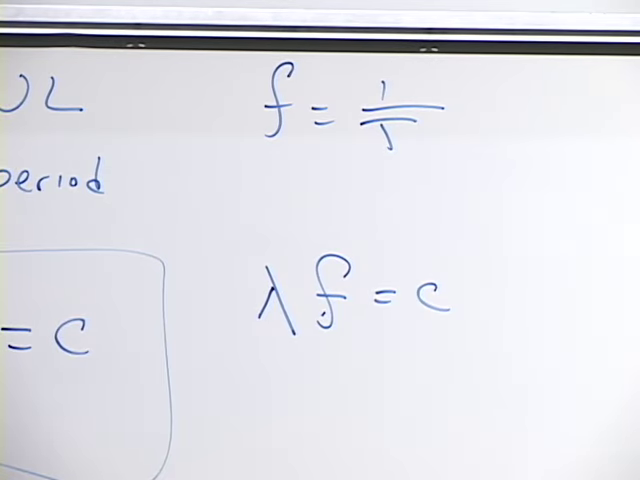
\includegraphics[width=0.68\textwidth]{lecture_01_figure_03.png}
\caption{Đối với sóng ánh sáng, \(f=1/T\) và \(\lambda f=c\).}
\lectureframe{00:36:24}
\end{figure}

Các nhà vật lý thường đo tốc độ dao động bằng radian trên giây thay vì bằng số chu kỳ trọn vẹn trên giây. Hãy hình dung chuyển động đều trên một đường tròn. Nếu điểm đó hoàn thành \(f\) vòng mỗi giây và mỗi vòng chứa \(2\pi\) radian, thì tần số góc của nó là
\begin{equation}
\omega=2\pi f,
\qquad
\frac{\omega}{2\pi}=f.
\end{equation}
Hiện giờ đây chỉ là một định nghĩa; câu hỏi thực hành rằng liệu nó có làm giảm số lượng các thừa số \(2\pi\) hay không sẽ quay lại sau.

Kết hợp \(f=c/\lambda\) với \(\omega=2\pi f\) ta được
\begin{equation}
\omega=\frac{2\pi c}{\lambda},
\qquad
\omega\lambda=2\pi c.
\end{equation}
Đối với một loại sóng khác, thay \(c\) bằng tốc độ lan truyền của sóng đó.

\begin{figure}[h]
\centering
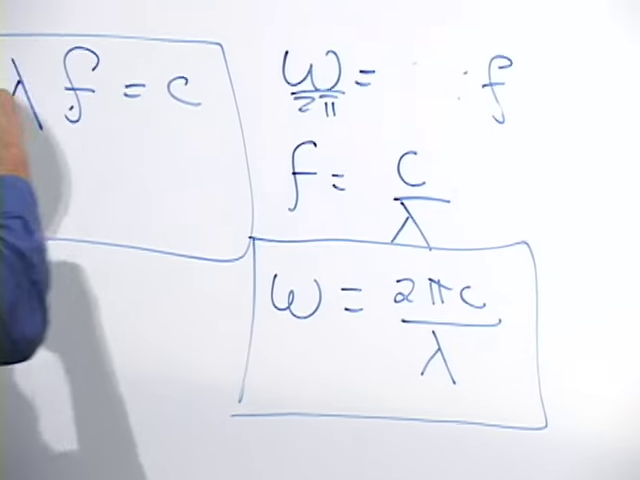
\includegraphics[width=0.68\textwidth]{lecture_01_figure_04.png}
\caption{Với \(\omega=2\pi f\), sóng ánh sáng thỏa mãn \(\omega=2\pi c/\lambda\).}
\lectureframe{00:39:10}
\end{figure}

Bức xạ điện từ tạo thành một phổ liên tục. Sắp theo thứ tự từ bước sóng dài hơn đến ngắn hơn, các tên gọi quy ước là
\begin{equation}
\begin{aligned}
\text{radio}
&\longrightarrow \text{microwave}
\longrightarrow \text{infrared}
\longrightarrow \text{visible}\\
&\longrightarrow \text{ultraviolet}
\longrightarrow \text{X ray}
\longrightarrow \text{gamma ray}.
\end{aligned}
\end{equation}
Ánh sáng khả kiến chỉ chiếm một khoảng hẹp. Ranh giới giữa các vùng được đặt tên là có tính quy ước, nên ở đây không cần các bước sóng phân chia chính xác. Sóng vô tuyến có thể cực kỳ dài; bức xạ gamma là đầu bước sóng rất ngắn của phổ điện từ. Khó khăn giờ đây trở nên sắc nét: bức xạ gamma về mặt cổ điển là một sóng trường liên tục, thế nhưng nó lại được phát hiện dưới dạng các tín hiệu rời rạc.

\section{Các lần đến rời rạc và xác suất do sóng chi phối}

Các tính chất nhiệt động lực học của bức xạ đã dẫn Planck và Einstein đến kết luận rằng ánh sáng phải được xử lý theo các đơn vị rời rạc. Một thí nghiệm tưởng tượng làm cho điểm này trở nên sinh động, nhưng đó không phải là một khẳng định về con đường lịch sử thực sự dẫn đến phát hiện ấy.

Chiếu một chùm tia lên một màn. Ở cường độ thông thường, nó tạo thành một đốm sáng trông như liên tục. Đặt một bộ suy giảm bán đục vào chùm tia: đốm sáng trở nên mờ hơn. Tăng độ suy giảm lặp đi lặp lại thì lượng ánh sáng đến trong mỗi đơn vị thời gian giảm đi. Cuối cùng, hình ảnh thay đổi. Thay vì một đốm mờ liên tục, bộ dò ghi nhận các sự kiện tách biệt.\footnote{Sơ đồ này tái dựng thí nghiệm suy giảm được triển khai trong video bài giảng trong khoảng từ 00:42:32 đến 00:45:42.}

\begin{figure}[h]
\centering
\begin{tikzpicture}[scale=0.9]
\begin{scope}
\draw[fill=yellow!35] (0,0) circle (0.18);
\draw[->,thick] (0.2,0) -- (2.55,0);
\draw[thick] (2.65,-1.0) -- (2.65,1.0);
\node[below] at (1.4,-1.0) {\small bright beam};
\end{scope}
\begin{scope}[xshift=4.1cm]
\draw[fill=yellow!35] (0,0) circle (0.18);
\draw[->,thick] (0.2,0) -- (1.15,0);
\draw[fill=gray!70] (1.2,-0.85) rectangle (1.55,0.85);
\draw[->,thick] (1.6,0) -- (2.55,0);
\draw[thick] (2.65,-1.0) -- (2.65,1.0);
\node[below] at (1.85,-1.0) {\small strong attenuation};
\end{scope}
\fill[gray!45] (2.62,-0.65) rectangle (2.70,0.65);
\foreach \y in {-0.66,-0.31,0.13,0.58}
  \fill (6.72,\y) circle (0.045);
\node[above] at (2.65,1.0) {\small unresolved exposure};
\node[above] at (6.75,1.0) {\small isolated detections};
\end{tikzpicture}
\caption{Sự suy giảm tăng dần làm giảm tốc độ phát hiện cho đến khi một ảnh phơi sáng trông như liên tục được phân giải thành các sự kiện photon riêng lẻ.}
\end{figure}

Chờ đủ lâu thì những sự kiện ấy tích lũy thành cùng một dạng phân bố không gian như đốm ban đầu. Vì vậy, vùng sáng là tổng chưa được phân giải của nhiều lần đến riêng lẻ. Thí nghiệm cường độ thấp này có thể thực hiện được, dù nó không phải là thí nghiệm thời kỳ đầu đã ban đầu thúc đẩy giả thuyết photon. Đề xuất photon của Einstein nảy sinh từ những xem xét nhiệt động lực học và quang điện; thí nghiệm suy giảm cung cấp một cách đặc biệt trực tiếp để hình dung hệ quả của nó.

Bây giờ hãy đặt hai lỗ mở trong chùm tia và giảm cường độ cho đến khi các photon đến từng cái một. Mỗi lần phát hiện là một vết chấm cục bộ. Thế nhưng sau nhiều lần phát hiện, các vết chấm ấy lấp đầy một hình giao thoa, gồm cả các vân sáng và tối. Các lần đến rời rạc là ngẫu nhiên, nhưng phân bố xác suất của chúng chính là phân bố do hình sóng dự đoán. Sóng cổ điển đã trở thành một sóng chi phối các xác suất.

Vì vậy, sóng và hạt không phải là hai loại thực thể tách biệt được gán cho những phần khác nhau của tự nhiên. Chúng là hai biểu hiện của cùng một đối tượng lượng tử. Không thể mô tả đầy đủ ánh sáng chỉ như sóng hoặc chỉ như hạt.

Electron đảo ngược điều ngạc nhiên ban đầu. Electron được chấp nhận là hạt và đến bộ dò từng cái một, nhưng với các lỗ mở đủ gần nhau chúng cũng tạo nên một hình giao thoa. Hạt alpha, nặng hơn electron khoảng 8000 lần, tuân theo cùng nguyên lý đó, mặc dù thí nghiệm khó hơn. Giao thoa thậm chí còn đã được quan sát với buckyball: các phân tử gồm 60 nguyên tử carbon được sắp xếp xấp xỉ như một dạng tổng quát của quả bóng đá. Nguyên lý ấy được kỳ vọng là áp dụng ngay cả cho các quả bóng bowling, mặc dù một thí nghiệm như vậy là cực kỳ bất khả thi về mặt thực hành. Có thể đẩy thảo luận xa hơn tới các thí nghiệm được đề xuất với virus hoặc tế bào sống như những ví dụ ngày càng táo bạo hơn. Hiểu được mô tả sóng và mô tả hạt ăn khớp với nhau như thế nào đòi hỏi cơ học lượng tử; nhiệm vụ trước mắt là rút ra các tính chất của photon cần cho vật lý hạt.

\section{Năng lượng photon}

Photon là những thành phần rời rạc, không thể chia của ánh sáng. Ánh sáng mang năng lượng---ánh sáng mặt trời làm nóng một vật hấp thụ---nên mỗi photon phải mang năng lượng. Một sóng đơn sắc có bước sóng và tần số góc xác định, và mỗi photon trong đó có
\begin{equation}
E_\gamma=\hbar\omega.
\end{equation}
Cố hình dung một sóng liên tục như một tập hợp cơ học gồm những chấm nhỏ là gây hiểu lầm. Điều xác định là sự kết hợp thực nghiệm sau: các phát hiện cục bộ xảy ra theo một phân bố do sóng chi phối, và năng lượng đến theo những đơn vị không thể chia.

Vì
\begin{equation}
\omega=\frac{2\pi c}{\lambda},
\end{equation}
một bước sóng ngắn hơn có nghĩa là một tần số góc lớn hơn và do đó nhiều năng lượng hơn trong mỗi photon:
\begin{equation}
\lambda\downarrow
\quad\Longrightarrow\quad
\omega\uparrow
\quad\Longrightarrow\quad
E_\gamma\uparrow.
\end{equation}
Một photon vô tuyến đơn lẻ có rất ít năng lượng. Tuy nhiên, một chùm vô tuyến vẫn có thể mang tổng năng lượng khổng lồ bằng cách chứa rất nhiều photon. Đối với một xung đơn sắc chứa \(n\) photon,
\begin{equation}
E_{\text{pulse}}=n\hbar\omega,
\qquad
n=0,1,2,\ldots.
\end{equation}
Tổng năng lượng có thể lớn, nhưng nó vẫn là một bội số nguyên của năng lượng một photon.

Hệ thức này dẫn tới câu hỏi thực tiễn sẽ chi phối phần còn lại của cuộc thảo luận. Tại sao phải xây những cỗ máy ngày càng lớn hơn để nhìn thấy những thứ ngày càng nhỏ hơn? Tại sao không dùng một cỗ máy nhỏ cho một vật nhỏ? Nửa đầu của câu trả lời đã có sẵn: phân giải cấu trúc nhỏ hơn đòi hỏi bước sóng ngắn hơn, và một lượng tử có bước sóng ngắn hơn mang năng lượng lớn hơn.

\section{Năng lượng nghỉ và khối lượng bất biến}

Vật lý hạt kết hợp cơ học lượng tử với thuyết tương đối. Hệ thức photon \(E_\gamma=\hbar\omega\) cung cấp phía lượng tử; sự kiện sơ đẳng tương ứng từ thuyết tương đối là
\begin{equation}
E_{\mathrm{rest}}=mc^2.
\end{equation}
Điều kiện kèm theo này rất quan trọng. Các trình bày cũ phân biệt \emph{khối lượng nghỉ} với \emph{khối lượng chuyển động} phụ thuộc vận tốc. Thuật ngữ hiện đại dùng \emph{khối lượng} để chỉ khối lượng bất biến của một vật. Chuyển động làm thay đổi năng lượng của nó, chứ không làm thay đổi khối lượng của nó. Mọi electron đều có cùng một khối lượng, bất kể trạng thái chuyển động của nó ra sao, trong khi năng lượng của electron tăng lên khi nó được gia tốc. Vì vậy, \(E=mc^2\), ở dạng này, là năng lượng của một vật có khối lượng trong một hệ quy chiếu mà toàn bộ vật đứng yên.

Vật không nhất thiết phải không có chuyển động nội tại. Một hộp khí có thể đứng yên trên cân trong khi các phân tử của nó chuyển động nhanh theo mọi hướng. Năng lượng của những chuyển động nội tại ấy là một phần của năng lượng nghỉ của toàn bộ chiếc hộp. Hãy bắt đầu với một chiếc hộp lạnh, đo khối lượng của nó, rồi thêm nhiệt năng trong khi vẫn giữ chính chiếc hộp đứng yên. Khối lượng nghỉ của nó thay đổi một lượng
\begin{equation}
\Delta m=\frac{\Delta E_{\mathrm{internal}}}{c^2}.
\end{equation}
Trọng lượng và quán tính của nó tăng cùng với khối lượng. Đối với một chiếc hộp thông thường, ngay cả sau khi nhiệt độ tăng nhiều, hiệu ứng ấy vẫn quá nhỏ để nhận ra trên một cái cân thông thường; độ nhỏ của hiệu ứng không làm thay đổi nguyên lý.

Một ví dụ sắc nét hơn xét một electron và một positron. Chúng có khối lượng bằng nhau chính xác và điện tích trái dấu. Nếu ban đầu chúng đứng yên và hủy nhau, các photon mang năng lượng đi:
\begin{equation}
e^-+e^+\longrightarrow \text{photons}.
\end{equation}
Năng lượng ban đầu là
\begin{equation}
E_{\mathrm{initial}}=2m_e c^2,
\end{equation}
và năng lượng đó không thể biến mất. Một cặp đơn lẻ chỉ cho một lượng cực nhỏ, nên cần một số lượng cặp khổng lồ mới có thể đun nóng dù chỉ một cốc cà phê, nhưng các sự kiện hủy riêng lẻ cho thấy trực tiếp sự chuyển đổi ấy.

Vì vậy, đối với một vật đứng yên, khối lượng và năng lượng là cùng một đại lượng vật lý được biểu diễn bằng các đơn vị khác nhau. Hệ số \(c^2\) là hệ số chuyển đổi giữa các đơn vị khối lượng và năng lượng thông dụng, cũng như một hệ số số học chuyển mét thành xentimét.

\begin{classroomqa}
\lecturetimestamp{01:04:39}
\audiencequestion{Việc chuyển khối lượng thành năng lượng được giải phóng có đòi hỏi một cơ chế không?}
\lecturerresponse{Có, cần một cơ chế vật lý, nhưng các định luật bảo toàn đã ràng buộc kết quả của nó. Ngay cả trước khi mô tả cơ chế hủy vi mô, năng lượng ban đầu của cặp electron--positron vẫn phải xuất hiện lại ở đâu đó. Vì vậy, bảo toàn năng lượng có thể quyết định một phần quan trọng của câu trả lời mà không cần trình bày chi tiết về tương tác.}
\end{classroomqa}

\section{Thứ nguyên và việc chọn đơn vị}

Trong hệ đơn vị SI, tốc độ ánh sáng là một số rất lớn và hằng số Planck là một số rất nhỏ. Độ nhỏ của đại lượng sau đã được gợi ra ngay bởi hệ thức photon: tần số góc của ánh sáng khả kiến là cực lớn trong khi năng lượng của một photon thì cực nhỏ, nên \(E_\gamma=\hbar\omega\) đòi hỏi \(\hbar\) phải có một giá trị số nhỏ trong các đơn vị này. Xét theo bậc độ lớn,
\begin{equation}
c\sim 10^8\ \mathrm{m\,s^{-1}},
\qquad
\hbar\sim 10^{-34}\ \mathrm{J\,s}.
\end{equation}
\editorialnote{Chỉ giữ lại các bậc độ lớn đã nêu trong bài giảng vì các chữ số cuối trên bảng không rõ.}
Các đơn vị là thiết yếu: không hằng số nào trong hai hằng số này chỉ đơn thuần là một số thập phân. Vì năng lượng có thứ nguyên
\begin{equation}
[E]=M L^2 T^{-2},
\end{equation}
và \(E_\gamma=\hbar\omega\) với \([\omega]=T^{-1}\), nên hằng số Planck có thứ nguyên
\begin{equation}
[\hbar]=[E]T=M L^2 T^{-1}.
\end{equation}

Việc gọi \(c\) là lớn và \(\hbar\) là nhỏ đã ngầm giả định một lựa chọn đơn vị. Đo tốc độ bằng foot trên giờ cho giá trị số của \(c\) khác với khi đo bằng mét trên giây. Tính theo năm ánh sáng trên năm, hoặc giây ánh sáng trên giây, tốc độ ánh sáng đơn giản là một. Tương tự, một lựa chọn phối hợp thích hợp của các đơn vị khối lượng, độ dài và thời gian cũng có thể làm cho \(\hbar=1\).

Các hệ đơn vị quen thuộc là những quy ước được thừa hưởng, không phải những đặc trưng được tự nhiên ưu đãi. Một dặm có 5280 foot, một stone có 14 pao, ngựa được đo bằng gang tay, và công suất có thể được đo bằng mã lực. Các đơn vị mét là có hệ thống hơn, nhưng thang của chúng vẫn là những lựa chọn của con người. Không có gì trong vật lý cơ bản khiến mét, giây hay kilôgam trở thành đơn vị đặc biệt.

Độ dài, thời gian và khối lượng cung cấp 3 lựa chọn đơn vị cơ bản độc lập:
\begin{equation}
L,\qquad T,\qquad M.
\end{equation}
Các đơn vị cơ học khác có thể được xây dựng từ chúng. Những lựa chọn hữu ích phụ thuộc vào bài toán. Một khối lượng Mặt Trời là thuận tiện trong vật lý thiên văn; một khối lượng proton có thể thuận tiện trong vật lý hạt nhân; năm ánh sáng và năm làm cho các công thức thiên văn tương đối tính trở nên gọn hơn. Với 3 lựa chọn độc lập, người ta có thể gán các giá trị số thuận tiện cho 3 hằng số có thứ nguyên độc lập. Vật lý thiên văn, vật lý nguyên tử và vật lý hạt không nhất thiết phải dùng cùng những lựa chọn đó.

Đối với vật lý hạt, 2 quy ước đặc biệt hữu ích là
\begin{equation}
c=1,
\qquad
\hbar=1.
\end{equation}
Không có một khối lượng hạt nào nổi bật tương đương cho đơn vị còn lại. Người ta có thể tuyên bố khối lượng proton, khối lượng boson Higgs hoặc khối lượng muon bằng một, nhưng như thế chỉ đơn thuần ưu ái một thành viên trong một tập hợp lớn.

Vậy tại sao lại chọn \(c\) và \(\hbar\)? Một câu trả lời đầu tiên có thể là chúng xuất hiện trong nhiều phương trình. Chỉ tần suất xuất hiện thì chưa đủ: khối lượng proton cũng xuất hiện trong nhiều phương trình, kích thước của proton cũng vậy. Điều làm \(c\) và \(\hbar\) khác biệt là tính phổ quát của chúng.

Các hằng số \(c\) và \(\hbar\) là khác loại. Tốc độ \(c\) ràng buộc mọi vật thể vật lý: các vật có khối lượng có thể tiến gần tới nó nhưng không thể được gia tốc để vượt qua nó. Hằng số Planck ràng buộc mọi đối tượng lượng tử thông qua hệ thức bất định theo bậc độ lớn
\begin{equation}
\Delta x\,\Delta p\gtrsim\hbar.
\end{equation}
Không phát biểu nào trong hai phát biểu ấy đặc cách một loại hạt cụ thể. Chính tính phổ quát này làm cho \(c=1\) và \(\hbar=1\) trở thành những quy ước tự nhiên.

Proton không cung cấp một thang chuẩn phổ quát tương đương. Nó chỉ là một vật trong rất nhiều vật. Đặt khối lượng proton bằng một không có địa vị cơ bản hơn gì việc đặt khối lượng của một nguyên tử rubidi bằng một; electron, boson Higgs và muon cũng gặp cùng khó khăn ấy.

Điện tích gợi ý một đại lượng phổ quát khác, nhưng sau khi \(c\) và \(\hbar\) đã được chuẩn hóa, hằng số ghép điện từ có ý nghĩa vật lý là vô thứ nguyên. Thay đổi đơn vị có thể dịch chuyển các hằng số có thứ nguyên qua lại trong một công thức điện từ; nó không thể thay đổi một hằng số ghép vô thứ nguyên thực sự.

Hấp dẫn cung cấp một hằng số phổ quát có thứ nguyên. Dưới dạng Newton, độ lớn của lực giữa hai khối lượng là
\begin{equation}
F=G\frac{m_1m_2}{r^2}.
\end{equation}
Mọi khối lượng đều hấp dẫn, trong khi các vật trung hòa điện không nhất thiết tham gia vào một lực điện. Vì vậy \(G\) có tính phổ quát cần thiết. Tuy nhiên, nó là một chuẩn hóa thực tiễn kém cho vật lý hạt thông thường, vì các lực hấp dẫn giữa những hạt cơ bản đã biết là không đáng kể trong các phép tính đang được bàn tới.

\begin{classroomqa}
\lecturetimestamp{01:20:34}
\audiencequestion{Có hợp lệ không nếu đơn giản gạt bỏ \(G\)? Ở năng lượng rất cao, các hạt cơ bản có thể không tuân theo hấp dẫn cổ điển theo cách đang được giả định.}
\lecturerresponse{Từng hạt riêng lẻ quả thực có phản ứng với trường hấp dẫn của Trái Đất: một hạt đơn lẻ rơi trong trường đó. Ảnh hưởng hấp dẫn của một hạt cơ bản này lên một hạt cơ bản khác chưa được đo trực tiếp, nên giả định về tính phổ quát có thể bị đặt dấu hỏi ở cấp độ ấy. Lý do trực tiếp để bỏ \(G\) ra ngoài mang tính thực tiễn hơn là tuyệt đối: hấp dẫn đóng góp không đáng kể vào các thí nghiệm và phương trình vật lý hạt thông thường.}
\end{classroomqa}

\begin{classroomqa}
\lecturetimestamp{01:22:01}
\audiencequestion{Liệu tương tác điện có thể được dùng làm quy ước ấn định đơn vị thứ ba thay cho hấp dẫn không?}
\lecturerresponse{Có. Ta có thể chọn các đơn vị điện từ trong đó điện tích, hoặc hằng số xuất hiện trong định luật Coulomb, được chuẩn hóa. Những quy ước như vậy quả có được sử dụng. Electron đẩy nhau chứ không hút nhau, nhưng dấu đó không cản trở lựa chọn này. Chỉ là đây không phải quy ước được dùng ở đây.}
\end{classroomqa}

\begin{classroomqa}
\lecturetimestamp{01:23:06}
\audiencequestion{Một khi \(c\) và \(\hbar\) được đặt bằng 1, điện tích có phải là vô thứ nguyên không?}
\lecturerresponse{Có. Một đại lượng vô thứ nguyên gắn với bình phương điện tích điện có giá trị xấp xỉ \(1/137\). Quy ước chính xác và ý nghĩa của con số đó có thể để lại bàn sau; điểm ở đây là nó vô thứ nguyên.}
\end{classroomqa}

\begin{classroomqa}
\lecturetimestamp{01:23:37}
\audiencequestion{Có thể chọn hằng số Coulomb làm hằng số thứ ba được đặt bằng 1 không?}
\lecturerresponse{Nó có thể được hấp thụ vào quy ước đơn vị điện từ. Lựa chọn đó không thể biến hằng ghép vô thứ nguyên \(1/137\) thành 1, vì đổi đơn vị không thể làm thay đổi một số vô thứ nguyên. Ở đây không khẳng định có lợi ích đặc biệt nào khi dùng quy ước đó.}
\end{classroomqa}

\section{Các phương trình trong đơn vị tự nhiên và các hệ quy chiếu}

Khi \(c=1\), hệ thức năng lượng nghỉ đối với một vật có khối lượng trở thành
\begin{equation}
E_{\mathrm{rest}}=m.
\end{equation}
Khi \(\hbar=1\), hệ thức cho photon trở thành
\begin{equation}
E_\gamma=\omega.
\end{equation}
Có thể khôi phục các hằng số bất cứ khi nào cần đến các giá trị số trong những đơn vị thông thường.

\begin{figure}[h]
\centering
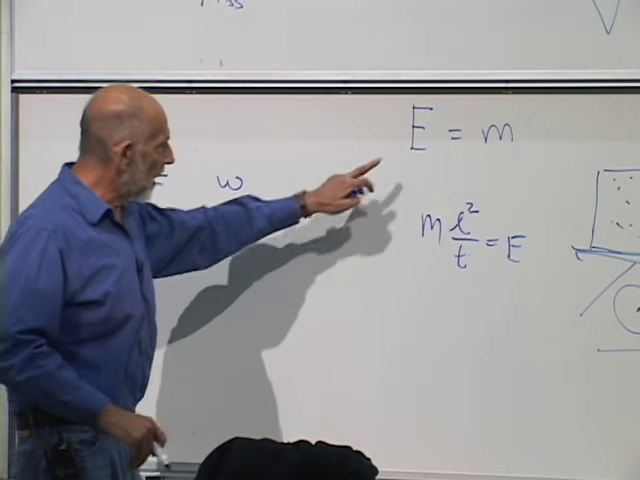
\includegraphics[width=0.72\textwidth]{lecture_01_figure_05.png}
\caption{Trong hệ đơn vị với \(c=1\), năng lượng nghỉ của một vật có khối lượng đứng yên là \(E=m\).}
\lectureframe{01:25:40}
\end{figure}

Những công thức này trông giống nhau nhưng mang ý nghĩa khác nhau. Trong \(E_{\mathrm{rest}}=m\), \(E\) là năng lượng nghỉ của một vật có khối lượng. Photon không có khối lượng và không thể được đưa về trạng thái nghỉ, nên năng lượng của nó không phải là năng lượng nghỉ. Hệ thức \(E_\gamma=\omega\) cho năng lượng của một lượng tử không khối lượng đang chuyển động.

\begin{classroomqa}
\lecturetimestamp{01:26:07}
\audiencequestion{\emph{đứng yên} có nghĩa là gì khi trạng thái nghỉ luôn là tương đối đối với một cái gì đó và bản thân phòng thí nghiệm cũng không tuyệt đối đứng yên?}
\lecturerresponse{Trạng thái nghỉ được định nghĩa tương đối với một hệ quy chiếu được chọn. Nếu một cái cốc đứng yên so với phòng thí nghiệm, thì trong hệ quy chiếu của phòng thí nghiệm đó, năng lượng của nó bằng khối lượng của nó khi \(c=1\), không có đóng góp động năng tổng thể nào. Một quan sát viên khác chuyển động ngang qua cái cốc sẽ gán cho nó cả động năng nữa. Nói chung, các quan sát viên khác nhau sẽ gán những năng lượng khác nhau cho cùng một vật hoặc cùng một photon; năng lượng phụ thuộc hệ quy chiếu, và không cần giả định có trạng thái nghỉ tuyệt đối.}
\end{classroomqa}

Giờ có thể xem xét lại quy ước dùng tần số góc. Viết \(E_\gamma=\hbar\omega\) thì gọn, nhưng \(\omega=2\pi f\) trước đó đã đưa vào một thừa số \(2\pi\).

\begin{classroomqa}
\lecturetimestamp{01:28:13}
\audiencequestion{Tại sao lại dùng tần số góc \(\omega\), đo bằng radian trên giây, thay vì số chu kỳ trọn vẹn mỗi giây có vẻ đơn giản hơn?}
\lecturerresponse{Lựa chọn này một phần mang tính lịch sử, và câu trả lời về mặt toán học là thực dụng hơn là trực tiếp. Câu trả lời được nêu ở đây chỉ có tính tạm thời: hãy viết các phương trình liên quan một lần với \(f\) và một lần với \(\omega\), rồi xem quy ước nào để lại ít thừa số \(2\pi\) hơn. Không thể làm cho các thừa số \(2\pi\) biến mất ở mọi nơi. Một mối liên hệ khả dĩ với ký hiệu mũ phức cũng đã được gợi ý, nhưng ở đây không triển khai.}
\end{classroomqa}

\begin{classroomqa}
\lecturetimestamp{01:29:51}
\audiencequestion{Có thể gia tốc hai hạt cho đến khi tương tác hấp dẫn lẫn nhau của chúng trở nên quan trọng không?}
\lecturerresponse{Về nguyên tắc, có. Trên thực tế, các máy gia tốc hiện nay còn cách chế độ đó một khoảng cực kỳ xa. Câu trả lời cũng phụ thuộc vào việc từ hạt được hiểu theo nghĩa nào: một vật vĩ mô gây hấp dẫn không phải là trường hợp hạt cơ bản đang được bàn tới.}
\end{classroomqa}

\begin{classroomqa}
\lecturetimestamp{01:30:27}
\audiencequestion{Nguồn positron có thể là gì?}
\lecturerresponse{Các va chạm năng lượng cao có thể tạo ra positron. Một số quá trình và phân rã hạt nhân cũng sinh ra chúng.}
\end{classroomqa}

\begin{classroomqa}
\lecturetimestamp{01:30:53}
\audiencequestion{Thời gian Planck và khoảng cách Planck có phải là các đơn vị tự nhiên đang được dùng ở đây không?}
\lecturerresponse{Không. Đơn vị Planck xuất hiện khi \(G\), \(c\) và \(\hbar\) đều được đặt bằng 1. Độ dài Planck thu được nhỏ hơn rất nhiều so với các thang độ dài của vật lý hạt thông thường, nên ở đây nó là một thước đo bất tiện. Những đơn vị như vậy là tự nhiên khi hấp dẫn, cơ học lượng tử và thuyết tương đối đều cùng quan trọng, như trong vật lý lỗ đen, vũ trụ học hoặc hấp dẫn lượng tử. Khi hấp dẫn có thể bỏ qua, việc chỉ đặt \(c\) và \(\hbar\) bằng 1 sẽ hữu ích hơn.}
\end{classroomqa}

\section{Động lượng, ánh sáng và độ phân giải}

Khái niệm cơ bản tiếp theo là động lượng. Một vật đứng yên không có động lượng, mặc dù nó có năng lượng nghỉ khác không là \(mc^2\). Một khi chuyển động, nói chung nó mang động lượng. Động lượng được bảo toàn trong va chạm cũng như năng lượng được bảo toàn: khi hai vật va chạm, tổng động lượng vectơ trước và sau va chạm là như nhau. Bất kỳ đại lượng nào bị ràng buộc bởi một định luật bảo toàn đều đáng được đặc biệt lưu ý.

Động lượng là một vectơ: nó hướng theo phương chuyển động. Đối với một vật phi tương đối tính,
\begin{equation}
\mathbf p=m\mathbf v.
\end{equation}
Đây không phải công thức tương đối tính tổng quát, và không thể áp dụng trực tiếp cho ánh sáng.

Tuy vậy, ánh sáng vẫn mang động lượng cũng như năng lượng. Ánh sáng thông thường tạo ra lực đẩy nhỏ đến mức khó nhận ra động lượng của nó, nhưng một xung laser cường độ mạnh có thể truyền một xung lượng đáng kể. Chẳng hạn, hệ laser lớn ở Livermore có thể đẩy vật chất vào trong bằng động lượng do bức xạ của nó mang theo.

Hãy xét một xung được chuẩn trực đủ tốt để các tia của nó truyền gần như dọc theo một trục. Một chùm thực có thể có một độ trải góc nào đó, với các phần truyền theo những hướng hơi khác nhau, nhưng đối với một chùm chuẩn trực lý tưởng thì động lượng hướng dọc theo chùm và có độ lớn
\begin{equation}
p=\frac{E}{c},
\qquad\text{or equivalently}\qquad
E=cp.
\end{equation}
Ở đây, hệ thức này được chấp nhận như một thực kiện tương đối tính chứ không được chứng minh. Phép kiểm tra thứ nguyên sau đây chỉ xác nhận rằng đơn vị của nó phù hợp với đơn vị của động lượng thông thường:
\begin{equation}
\left[\frac{E}{c}\right]
=
\frac{M L^2 T^{-2}}{L T^{-1}}
=
M L T^{-1}
=
[m v]
=
[p].
\end{equation}
Phép so sánh thứ nguyên này không gán khối lượng nghỉ cho ánh sáng. Photon có khối lượng bằng 0; nó mang động lượng vì nó mang năng lượng và chuyển động với \(c\).

Phương của \(\mathbf p\) là phương truyền. Độ lớn của nó thường khó phát hiện vì \(c\) xuất hiện ở mẫu số. Một chùm có thể dễ dàng bộc lộ năng lượng của nó bằng cách nung nóng hoặc làm bay hơi vật chất, trong khi lực đẩy cơ học của nó nhỏ hơn nhiều. Tuy nhiên, với cường độ đủ lớn, lực đẩy đó có thể trở nên đáng kể.

Đối với một photon,
\begin{align}
p_\gamma
&=\frac{E_\gamma}{c}\\
&=\frac{\hbar\omega}{c}.
\end{align}
Để biểu diễn điều này theo bước sóng, hãy quay lại cẩn thận với các hệ thức sóng. Vì
\begin{equation}
f\lambda=c,
\qquad
\omega=2\pi f,
\end{equation}
hệ thức đúng là
\begin{equation}
\omega\lambda=2\pi c,
\qquad
\omega=\frac{2\pi c}{\lambda}.
\end{equation}
Thừa số \(2\pi\) rất dễ bị đảo ngược nếu không viết tường minh các định nghĩa. Bắt đầu lại từ \(f\lambda=c\) và \(f=\omega/(2\pi)\) sẽ giải quyết dứt điểm vấn đề:
\begin{equation}
\frac{\omega}{2\pi}\lambda=c
\quad\Longrightarrow\quad
\omega\lambda=2\pi c.
\end{equation}
Thế vào bây giờ cho
\begin{align}
p_\gamma
&=\frac{\hbar}{c}\frac{2\pi c}{\lambda}\\
&=\frac{2\pi\hbar}{\lambda}\\
&=\frac{h}{\lambda}.
\end{align}

\begin{classroomqa}
\lecturetimestamp{01:42:38}
\audiencequestion{\(2\pi\hbar\) có bằng \(h\) không?}
\lecturerresponse{Có. Theo định nghĩa \(h=2\pi\hbar\), nên \(p_\gamma=2\pi\hbar/\lambda\) cũng chính là \(p_\gamma=h/\lambda\). Các thừa số \(2\pi\) sẽ xuất hiện trở lại ở đâu đó, bất kể chọn quy ước tần số nào.}
\end{classroomqa}

Bước sóng càng ngắn thì động lượng của photon càng lớn. Một photon vô tuyến có bước sóng rất dài và động lượng cực nhỏ. Một photon tia gamma có bước sóng rất ngắn và cú hích lớn hơn nhiều. Một photon đơn lẻ vẫn chỉ tạo ra một xung lượng vĩ mô nhỏ, nhưng động lượng của nó lớn hơn rất nhiều so với photon vô tuyến. Năng lượng của nó cũng lớn hơn, vì \(E_\gamma=cp_\gamma\).

Hệ thức này giải thích vì sao những vật nhỏ hơn đòi hỏi những cỗ máy lớn hơn. Một bức ảnh được tạo bằng các bước sóng dài hơn nhiều so với đầu người thì chỉ có thể cho ra một vệt mờ. Để phân biệt các nét trên khuôn mặt, bước sóng phải ngắn hơn đầu. Để phân giải một sợi tóc, nó phải cỡ bằng hoặc nhỏ hơn bề dày của sợi tóc. Để phân giải cấu trúc của một nguyên tử, bước sóng của đầu dò phải không lớn hơn nguyên tử:
\begin{equation}
\lambda_{\mathrm{probe}}\lesssim
\text{size of the structure to be resolved}.
\end{equation}
Vì vậy, những cấu trúc nhỏ hơn đòi hỏi bước sóng ngắn hơn, và bước sóng ngắn hơn đòi hỏi động lượng và năng lượng lớn hơn. Đầu dò không nhất thiết phải là photon; các hạt năng lượng cao thuộc những loại khác cũng tuân theo cùng mối liên hệ lượng tử giữa bước sóng và động lượng. Việc tạo ra chúng đòi hỏi các máy gia tốc truyền ngày càng nhiều năng lượng cho mỗi hạt. Cặp \(p_\gamma=h/\lambda\) và \(E_\gamma=\hbar\omega\) làm rõ lập luận này: tăng năng lượng của đầu dò sẽ làm tăng động lượng của nó và rút ngắn bước sóng của nó.

Đây là mô thức lặp đi lặp lại của vật lý hạt trong khoảng một thế kỷ: năng lượng cao hơn, động lượng lớn hơn, bước sóng ngắn hơn và độ phân giải không gian tốt hơn.

\begin{classroomqa}
\lecturetimestamp{01:46:57}
\audiencequestion{Có giới hạn dưới về mặt lý thuyết đối với bước sóng không?}
\lecturerresponse{Có thể có. Người ta kỳ vọng sẽ có điều gì đó mới ở gần độ dài Planck, nhưng câu trả lời vẫn chỉ là tạm thời. Nếu độ phân giải không gian chạm đáy ở đó, thì thang ấy vẫn còn nhỏ hơn khoảng cách đang được thăm dò tại LHC khoảng 17 bậc độ lớn, nên các thí nghiệm hiện nay vẫn còn cách nó một khoảng khổng lồ.}
\end{classroomqa}

Cùng chuỗi lập luận ấy gợi ra một mối liên hệ gần đúng giữa quy mô của một máy gia tốc và thang mà nó có thể phân giải.

\begin{classroomqa}
\lecturetimestamp{01:48:02}
\audiencequestion{Bước sóng, hay kích thước đang được phân giải, có gần đúng tỉ lệ nghịch với kích thước của máy gia tốc không?}
\lecturerresponse{Đại thể là có, miễn là các điện trường cực đại dùng để gia tốc các hạt, và các từ trường dùng để dẫn hướng chúng, vẫn được giữ gần như cố định bởi thiết bị hiện có. Gradient gia tốc là độ tăng năng lượng trên một đơn vị chiều dài. Đối với một máy gia tốc thẳng có chiều dài \(L\) và gradient xấp xỉ cố định \(\mathcal G\),
\[
E_{\mathrm{beam}}\sim \mathcal G L.
\]
Ở năng lượng siêu tương đối tính, bước sóng có thể phân giải tỉ lệ nghịch với năng lượng, nên tăng chiều dài của máy gia tốc thẳng sẽ cải thiện độ phân giải xấp xỉ theo hệ số nghịch đảo đó. Đây chỉ là một quy luật tỉ lệ mang tính gợi ý, không phải một định luật chính xác. Máy gia tốc tròn cho phép đi qua cùng một thiết bị nhiều lần, nhưng các điện tích được gia tốc sẽ bức xạ khi bị bẻ cong và mất năng lượng.}
\end{classroomqa}

\begin{classroomqa}
\lecturetimestamp{01:49:47}
\audiencequestion{Máy gia tốc sẽ phải lớn đến mức nào để đạt tới độ dài Planck?}
\lecturerresponse{Theo cách tỉ lệ gần đúng này, nó sẽ phải dài hơn máy gia tốc của CERN khoảng 17 bậc độ lớn. Đó không phải là kích thước của vũ trụ, nhưng đại khái là ở quy mô thiên hà.}
\end{classroomqa}

\begin{classroomqa}
\lecturetimestamp{01:50:09}
\audiencequestion{Năng lượng của các tia vũ trụ năng lượng cao nhất so với năng lượng của các máy va chạm như thế nào?}
\lecturerresponse{Từng tia vũ trụ riêng lẻ có thể có năng lượng trong hệ phòng thí nghiệm lớn hơn nhiều. Để so sánh định lượng, hãy xét một tia vũ trụ cực hạn có năng lượng trong hệ phòng thí nghiệm cỡ \(10^{21}\,\mathrm{eV}=10^{12}\,\mathrm{GeV}\). Nhưng một tia vũ trụ đập vào một bia đứng yên trong phòng thí nghiệm, trong khi máy va chạm cho hai chùm hạt năng lượng cao va vào nhau trực diện. Quan trọng hơn, các thí nghiệm hữu ích đòi hỏi thông lượng: nhiều hạt và nhiều va chạm được kiểm soát tốt. Một tia vũ trụ đơn lẻ có thể trượt bia thích hợp hoặc tạo ra một sự kiện mà từ đó hầu như không thể suy ra được gì. Một ước tính quy đổi theo dầu mỏ mang tính cố ý phóng đại đã đặt mức cung cần thiết để vận hành một máy gia tốc thiên hà hữu ích vào khoảng một trăm nghìn tỷ thùng dầu mỗi giây. Mục đích của nó là cho thấy rằng việc có đủ thống kê va chạm sẽ là một trở ngại ít nhất cũng nghiêm trọng như chiều dài của máy gia tốc.}
\end{classroomqa}

\editorialnote{Ước tính quy đổi theo dầu mỏ không nhất quán trong nguồn. Ban đầu nó được nêu ra rồi được lặp lại là khoảng \(10^{14}\) thùng mỗi giây; một lần diễn đạt lại về sau cho \(10^{11}\) thùng mỗi giây. Cả hai thang bậc ấy đều được giữ lại, thay vì âm thầm hiệu chỉnh cho khớp với nhau.}

Đây là những thang khoảng cách thực, không chỉ đơn thuần là hình thức. Bài toán thực tiễn là làm thế nào thăm dò chúng mà không phải xây dựng một máy gia tốc cấp thiên hà và cung cấp cho nó mức công suất gần như hoang đường ấy.

\begin{classroomqa}
\lecturetimestamp{01:52:55}
\audiencequestion{Năng lượng của LHC nên được so sánh như thế nào với một tia vũ trụ có năng lượng \(10^{12}\,\mathrm{GeV}\)?}
\lecturerresponse{Đối với một hạt tới siêu tương đối tính có năng lượng trong hệ phòng thí nghiệm \(E_{\mathrm{lab}}\) đập vào một bia cố định có khối lượng \(m_{\mathrm{target}}\), năng lượng khối tâm phụ thuộc theo tham số như sau:
\[
E_{\mathrm{cm}}\simeq
\sqrt{2m_{\mathrm{target}}c^2E_{\mathrm{lab}}}.
\]
\editorialnote{Biểu thức cho trường hợp bia cố định được trình bày ở trên làm tường minh sự phụ thuộc theo căn bậc hai đã được nêu trong phần trao đổi.}
Khi khối lượng của bia được giữ cố định, năng lượng va chạm hữu ích vì thế chỉ tăng theo căn bậc hai của năng lượng hạt tới. Do đó, ở mức bậc độ lớn, một tia vũ trụ \(10^{12}\,\mathrm{GeV}\) tương ứng với năng lượng của các chùm ngược chiều cỡ \(10^6\,\mathrm{GeV}\) cho mỗi chùm, chứ không phải \(10^{12}\,\mathrm{GeV}\) trong mỗi chùm. Tia vũ trụ vẫn có thể vượt năng lượng của các máy va chạm trên Trái Đất, nhưng thông lượng rất thấp của chúng khiến các thí nghiệm có hệ thống và được kiểm soát trở nên không thực tế.}
\end{classroomqa}
\chapter{Sóng, các mode lượng tử hóa và toán tử tạo}

\section{Sóng, trường và các hàm mũ phức}

Lý thuyết trường lượng tử là công cụ cơ bản của vật lý hạt. Trước khi trình bày dù chỉ ở mức sơ cấp về một trường lượng tử, sẽ hữu ích nếu tập hợp lại các kết quả toán học kết nối sóng với hạt. Bản thân sóng đã là một cấu hình trường: một trường biến thiên từ điểm này sang điểm khác trong không gian, và sóng là một cấu hình trong đó các giá trị ấy dao động và lan truyền. Cơ học lượng tử cung cấp mối liên hệ giữa những sóng như vậy và các hạt.

Ở đây giả thiết người đọc đã có nền tảng về cơ học lượng tử và thuyết tương đối hẹp. Mục đích trước mắt là ôn lại những mảnh ghép cần cho vật lý hạt, chứ không thay thế một khóa học về bất kỳ môn nào trong hai môn đó.

Hàm mũ được đặc trưng bởi sự tăng trưởng tỉ lệ. Nếu
\begin{equation}
f(x)=e^{\alpha x},
\end{equation}
thì
\begin{equation}
\frac{df}{dx}=\alpha f.
\end{equation}
Trên một khoảng nhỏ, độ tăng tỉ lệ với lượng đã có sẵn. Một quần thể tăng trưởng trong đĩa Petri cho hình dung quen thuộc: càng có nhiều sinh vật hiện diện thì càng có nhiều cá thể có thể sinh sản, nên tốc độ tăng tỉ lệ với chính quần thể đó. Nhân \(e^{\alpha x}\) với một hằng số chung không làm thay đổi tính chất đặc trưng này.

Sin và cos dao động thay vì tăng trưởng. Chúng là cùng một đường cong nhưng lệch nhau một phần tư chu kỳ, và phép đạo hàm quay chúng thành nhau:
\begin{align}
\frac{d}{dx}\sin(kx)&=k\cos(kx),\\
\frac{d}{dx}\cos(kx)&=-k\sin(kx).
\end{align}
Mỗi hàm riêng lẻ đều không phải là một hàm mũ, vì đạo hàm của nó tỉ lệ với hàm kia. Tổ hợp phức thì có tính chất hàm mũ. Với \(i^2=-1\),
\begin{align}
\frac{d}{dx}\bigl(\cos(kx)+i\sin(kx)\bigr)
&=-k\sin(kx)+ik\cos(kx)\\
&=ik\bigl(\cos(kx)+i\sin(kx)\bigr).
\end{align}
Do đó
\begin{equation}
e^{ikx}=\cos(kx)+i\sin(kx).
\end{equation}
Đồng nhất thức này xuất hiện lặp đi lặp lại vì sin và cos mô tả các dao động dạng sóng. Khi \(x\) là một tọa độ không gian, hàm dao động theo không gian. Khi đối số là thời gian, nó dao động theo thời gian.

\section{Tần số, bước sóng và động lượng của photon}

Tần số thông thường \(f\) là số chu kỳ trọn vẹn trong mỗi giây. Một chu kỳ nghĩa là một dao động đầy đủ. Tần số góc đo cùng chuyển động ấy bằng radian trên giây:
\begin{equation}
\omega=2\pi f.
\end{equation}
Hai ký hiệu này mô tả cùng một tần số. Người ta chuyển qua lại giữa chúng để tránh đưa những thừa số \(2\pi\) không cần thiết vào phép tính, dù các thừa số ấy không bao giờ biến mất hoàn toàn.

Bước sóng \(\lambda\) là quãng đường chiếm bởi một chu kỳ không gian hoàn chỉnh. Nếu một sóng lan truyền với tốc độ \(v\), thì quãng đường trên mỗi chu kỳ nhân với số chu kỳ mỗi giây chính là tốc độ lan truyền:
\begin{equation}
\lambda f=v.
\end{equation}
Đối với ánh sáng trong chân không, \(v=c\), nên
\begin{equation}
\lambda f=c.
\end{equation}
Đối với sóng âm, vế phải là tốc độ âm thanh; còn đối với sóng nước, đó là tốc độ sóng nước thích hợp. Vì vậy, sự xuất hiện của \(c\) là một phát biểu về ánh sáng, chứ không phải một định nghĩa chung cho mọi sóng.

Cơ học lượng tử đưa vào hằng số Planck dưới hai ký hiệu,
\begin{equation}
\hbar=\frac{h}{2\pi}.
\end{equation}
Việc đổi từ \(h\) sang \(\hbar\) chỉ đơn thuần chuyển các thừa số \(2\pi\) từ phương trình này sang phương trình khác.

Giá trị số của các hằng số có thứ nguyên phụ thuộc vào hệ đơn vị dùng để biểu diễn chúng. Mét, giây và kilôgam là những quy ước theo thang kích thước của con người, thuận tiện cho các độ dài và thời gian thông thường. Các đơn vị truyền thống cỡ chiều dài một cánh tay từng hữu ích cho vải hoặc dây; dù con đường lịch sử chính xác dẫn đến mét là gì, không có nguyên lý cơ bản nào chọn ra đúng thang kích thước con người cụ thể này. Trong đơn vị SI,
\begin{equation}
\begin{aligned}
h &\simeq 6.6\times10^{-34}\ \mathrm{J\,s},
&\hbar &\simeq 1.1\times10^{-34}\ \mathrm{J\,s},\\
c &\simeq 3\times10^8\ \mathrm{m\,s^{-1}}.
\end{aligned}
\end{equation}
Điều cốt yếu của các con số này là thang độ của chúng trong các đơn vị quy ước: hằng số Planck nhỏ một cách khác thường và tốc độ ánh sáng lớn một cách khác thường.

Một lượng tử của một mode có năng lượng
\begin{equation}
E_{\text{one quantum}}=\hbar\omega=hf.
\end{equation}
Đây là năng lượng của một photon, không phải tổng năng lượng của một sóng điện từ cổ điển bất kỳ. Ánh sáng khả kiến có tần số cỡ \(10^{15}\) chu kỳ mỗi giây, nên một photon quang học điển hình có năng lượng cỡ
\begin{equation}
E_\gamma\sim 10^{-19}\ \mathrm{J}.
\end{equation}
Ngay cả một dao động quang học nhanh như vậy cũng cho năng lượng trên mỗi lượng tử rất nhỏ vì \(h\) quá nhỏ. Vì thế, một lượng năng lượng quang học vĩ mô chứa một số photon khổng lồ.

Năng lượng và động lượng đáng được chú ý đặc biệt vì cả hai đều được bảo toàn. Chúng là những đại lượng ghi sổ hữu ích: tổng năng lượng và động lượng đi vào một quá trình phải được cân bằng bởi tổng năng lượng và động lượng đi ra khỏi nó. Động lượng là một vectơ và hướng theo chiều chuyển động. Đối với một hạt chuyển động chậm hơn ánh sáng rất nhiều,
\begin{equation}
\vec p=m\vec v.
\end{equation}

Bây giờ hãy xét bức xạ điện từ được chuẩn trực theo một hướng, thay vì phân tán ra nhiều hướng. Động lượng của nó hướng dọc theo chùm. Công thức phi tương đối tính không thể áp dụng cho photon, vì \(m\) nghĩa là khối lượng nghỉ và photon có khối lượng nghỉ bằng 0. Tuy vậy vẫn có một cách ghi nhớ theo thứ nguyên hữu ích. Nếu người ta gán cho photon, một cách \emph{không thích hợp}, đại lượng \(E/c^2\) như thể đó là một khối lượng rồi sau đó thế \(v=c\), thì được
\begin{equation}
mv\longrightarrow \frac{E}{c^2}c=\frac{E}{c}.
\end{equation}
Thao tác này tình cờ cho ra đáp án đúng và cho đúng đơn vị, nhưng nó không phải là một lập luận hợp lệ cho thấy photon có khối lượng nghỉ \(E/c^2\). Phát biểu tương đối tính đúng cho bức xạ được chuẩn trực theo một hướng là
\begin{equation}
|\vec p|=\frac{E}{c}.
\end{equation}
Phương trình này cho độ lớn. Hướng là hướng mà bức xạ truyền đi.

Đối với một photon,
\begin{align}
|\vec p_\gamma|
&=\frac{E_\gamma}{c}
=\frac{hf}{c}.
\end{align}
Đối với ánh sáng,
\begin{equation}
\lambda f=c,
\qquad
\frac{f}{c}=\frac{1}{\lambda},
\end{equation}
và do đó
\begin{equation}
|\vec p_\gamma|=\frac{hf}{c}=\frac{h}{\lambda}.
\end{equation}

\begin{figure}[t]
\centering
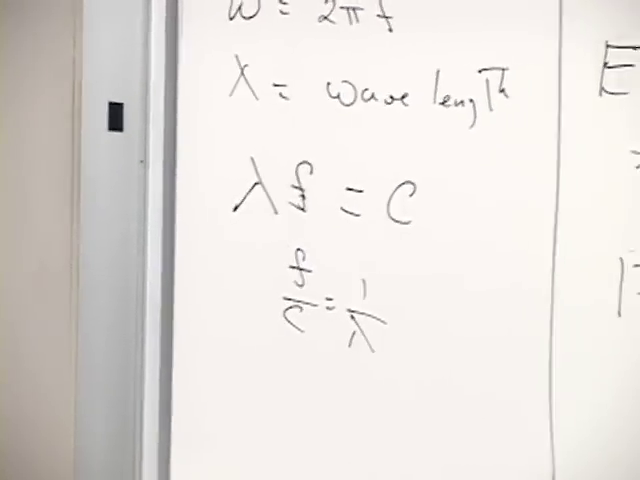
\includegraphics[width=0.56\textwidth]{lecture_02_figure_02.png}
\caption{Đối với ánh sáng, \(\lambda f=c\) và \(f/c=1/\lambda\) là các hệ thức dùng để suy ra \(|\vec p_\gamma|=h/\lambda\).}
\lectureframe{00:21:39}
\end{figure}

Bước sóng càng ngắn thì động lượng photon càng lớn. Đây là một trong những sự kiện lượng tử quan trọng nhất đối với vật lý hạt. Muốn nghiên cứu một vật nhỏ thì cần một đầu dò có bước sóng ngắn, và cái giá của bước sóng ngắn ấy là động lượng lớn.

\begin{classroomqa}
\lecturetimestamp{00:22:23}
\audiencequestion{Liệu \(E=\hbar\omega\) là cơ bản, hay được suy ra từ một nguyên lý sâu hơn?}
\lecturerresponse{Nó suy ra từ cơ học lượng tử của dao động tử điều hòa. Ở đây sẽ dùng kết quả đó mà không lặp lại chứng minh của nó; ngôn ngữ dao động tử được phát triển bên dưới cho bối cảnh sâu hơn của kết quả ấy.}
\end{classroomqa}


\section{Biên độ sóng và số photon}

\begin{classroomqa}
\lecturetimestamp{00:23:10}
\audiencequestion{Biên độ của một sóng có nghĩa gì trong ngôn ngữ photon?}
\lecturerresponse{Hãy so sánh hai sóng có cùng bước sóng và tần số nhưng biên độ khác nhau, chẳng hạn \(\sin(kx)\) và \(A\sin(kx)\). Theo cổ điển, năng lượng trong một vùng cố định tỉ lệ với bình phương biên độ. Theo lượng tử, một mode chứa \(n\) photon có năng lượng \(n\hbar\omega\). Vì vậy, khi giữ cố định tần số, vùng xét và chuẩn hóa, biên độ tăng theo bậc độ lớn như \(\sqrt n\).}
\end{classroomqa}

Hai sóng này giống hệt nhau về dạng dao động. Chỉ là một sóng mạnh hơn sóng kia.\footnote{Sơ đồ này theo phép so sánh sóng tại 00:23:47--00:24:28.}

\begin{figure}[t]
\centering
\begin{tikzpicture}[x=1cm,y=0.65cm]
\draw[->] (-0.4,0) -- (6.8,0);
\draw[->] (-0.4,-2.1) -- (6.8,-2.1);
\draw[thick] plot[domain=0:6.2,samples=120] (\x,{0.45*sin(\x r)});
\draw[thick] plot[domain=0:6.2,samples=120] (\x,{-2.1+1.15*sin(\x r)});
\draw (6.2,0.55) node[right]{small amplitude};
\draw (6.2,-0.75) node[right]{large amplitude};
\end{tikzpicture}
\caption{Các sóng có cùng bước sóng và tần số nhưng biên độ khác nhau.}
\end{figure}

Với một lượng sóng cố định,
\begin{equation}
E_{\text{wave}}\propto A^2.
\end{equation}
Đối với sóng điện từ, đây là phát biểu quen thuộc rằng năng lượng trường tỉ lệ với bình phương cường độ trường. Nếu cùng mode đó chứa \(n\) photon, thì
\begin{equation}
E_{\text{wave}}=n\hbar\omega.
\end{equation}
Do đó, khi giữ cố định mode, tần số, chuẩn hóa và vùng xét,
\begin{equation}
A^2\propto n\hbar\omega,
\qquad
A\propto\sqrt n\quad\text{at fixed }\omega.
\end{equation}
Ở đây không hề khẳng định một quy ước chuẩn hóa chính xác nào. Bao nhiêu phần của sóng được tính vào là điều quan trọng: gấp đôi chiều dài của một sóng đồng đều về mọi mặt khác sẽ làm thay đổi tổng năng lượng của nó mà không làm thay đổi biên độ cục bộ. Vì thế, phép tỉ lệ này có thể được hiểu cho một vùng cố định, chẳng hạn một bước sóng.

Cũng có một bảo lưu riêng của cơ học lượng tử. Biên độ và pha không thể đồng thời được gán các giá trị cổ điển chính xác. Vì thế câu hỏi ``Biên độ của một photon là bao nhiêu?'' là mơ hồ nếu nó đòi hỏi một trường cổ điển được xác định hoàn toàn. Tuy vậy, đặt \(n=1\) vẫn cho một thang bậc độ lớn hợp lý.

\begin{classroomqa}
\lecturetimestamp{00:28:25}
\audiencequestion{Độ lệch thẳng đứng trong một hình vẽ sóng điện từ có biểu diễn vị trí của photon trong không gian không?}
\lecturerresponse{Không. Trục lan truyền là trục không gian, còn tọa độ thẳng đứng biểu diễn giá trị của trường điện hoặc trường từ. Động lượng hướng dọc theo trục lan truyền, không dọc theo biên độ trường được vẽ ra.}
\end{classroomqa}

Sóng có thể lan truyền theo bất kỳ hướng không gian nào, nhưng hình sin quen thuộc chỉ dùng trục ngang của nó làm một tọa độ không gian. Hướng còn lại trên hình ghi lại cường độ trường.

\begin{classroomqa}
\lecturetimestamp{00:29:37}
\audiencequestion{Số photon được nêu đang được đếm trong một bước sóng hay một chu kỳ của sóng?}
\lecturerresponse{Ta có thể chọn một vùng cố định, chẳng hạn một bước sóng. Đó là lý do quan hệ chỉ là tỉ lệ: tổng năng lượng và số photon còn phụ thuộc vào việc lấy bao nhiêu phần của sóng vào. 2, 3 hoặc 4 bước sóng tương ứng chứa nhiều năng lượng hơn 1 bước sóng ở cùng biên độ.}
\end{classroomqa}

\begin{classroomqa}
\lecturetimestamp{00:30:17}
\audiencequestion{Biên độ của một photon đơn lẻ có vô nghĩa không?}
\lecturerresponse{Nó chỉ có ý nghĩa như một phát biểu về bậc độ lớn thu được bằng cách đặt \(n=1\). Đối với một mode điện từ, thông tin về điện trường và từ trường đóng vai trò tương tự như thông tin liên hợp về vị trí và động lượng, nên độ bất định lượng tử giới hạn mức độ sắc nét mà người ta có thể gán cho một biên độ cổ điển. Quan hệ ở mức bậc độ lớn vẫn hữu ích.}
\end{classroomqa}

Những câu hỏi này đã dẫn vào lý thuyết trường lượng tử, nơi mối liên hệ giữa các biến trường và số hạt có thể được phát biểu một cách chính xác. Còn hiện tại, các quan hệ tỉ lệ là đủ.

\section{Các quan hệ lượng tử tổng quát và sóng vật chất chuyển động chậm}

Một số công thức được giới thiệu cho photon áp dụng tổng quát hơn nhiều, còn những công thức khác thì không. Nên phân loại chúng trước khi chuyển sang electron.

\begin{figure}[t]
\centering
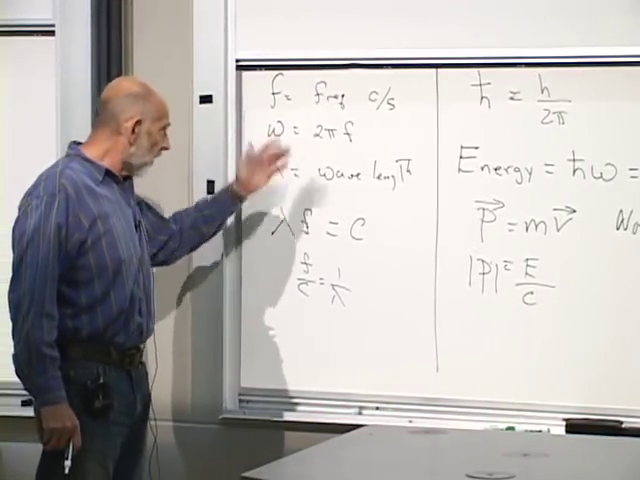
\includegraphics[width=0.82\textwidth]{lecture_02_figure_03.png}
\caption{Các định nghĩa về sóng và các hệ thức động lượng cho photon cũng như cho trường hợp phi tương đối tính, được so sánh theo miền hiệu lực của chúng.}
\lectureframe{00:31:52}
\end{figure}

Các định nghĩa của \(f\), \(\omega=2\pi f\) và \(\lambda\) áp dụng nói chung. Quan hệ lượng tử
\begin{equation}
E=\hbar\omega=hf
\end{equation}
cũng có tính tổng quát trong thảo luận hiện tại. Trái lại, các công thức chứa \(c\), chẳng hạn \(\lambda f=c\) và \(|\vec p|=E/c\), áp dụng cho các sóng chuyển động với tốc độ ánh sáng. Công thức \(\vec p=m\vec v\) áp dụng cho các hạt chuyển động chậm hơn ánh sáng rất nhiều. Chuyển động tương đối tính nằm giữa các giới hạn đó đòi hỏi một phép nội suy mà hiện chưa cần đến.

Quan hệ động lượng--bước sóng vẫn còn đúng ngoài ví dụ photon:
\begin{equation}
p=\frac{h}{\lambda}.
\end{equation}
Ở đây \(p\) ký hiệu độ lớn khi \(\lambda\) được lấy là một bước sóng dương; hướng có thể được bổ sung riêng.

\begin{figure}[t]
\centering
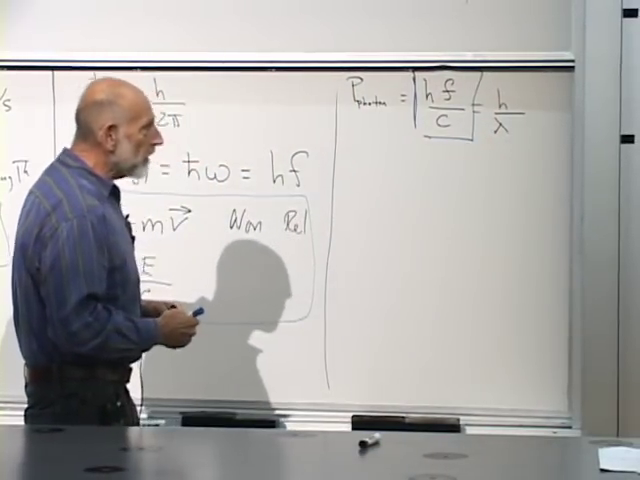
\includegraphics[width=0.74\textwidth]{lecture_02_figure_04.png}
\caption{Động lượng photon \(|\vec p_\gamma|=hf/c=h/\lambda\), dẫn đến hệ thức de Broglie tổng quát.}
\lectureframe{00:33:32}
\end{figure}

Có thể gắn một sóng với electron, hạt nhân, và thậm chí cả một quả bóng bowling. Giao thoa electron là một biểu hiện của điều đó. Ký hiệu sóng electron là \(\psi\). Đối với một electron chuyển động chậm, hệ thức nào thay thế \(\lambda f=c\)? Thành phần còn thiếu là quan hệ phi tương đối tính giữa năng lượng và động lượng.

Bắt đầu với động năng và động lượng:
\begin{align}
E&=\frac12 mv^2,\\
p&=mv,
\qquad
v=\frac{p}{m}.
\end{align}
Thế hệ thức cuối vào hệ thức đầu cho
\begin{align}
E
&=\frac12m\left(\frac{p}{m}\right)^2\\
&=\frac{p^2}{2m}.
\end{align}
Khối lượng nằm ở tử trong \(\frac12 mv^2\) và ở mẫu trong \(p^2/(2m)\). Vị trí ấy dễ nhầm lẫn, nên việc tự suy ra lại khá hữu ích.

Bây giờ dùng các quan hệ lượng tử tổng quát
\begin{equation}
E=hf,
\qquad
p=\frac{h}{\lambda}.
\end{equation}
Đối với một hạt chuyển động chậm đơn lẻ,
\begin{align}
hf
&=\frac{p^2}{2m}\\
&=\frac{1}{2m}\left(\frac{h}{\lambda}\right)^2\\
&=\frac{h^2}{2m\lambda^2}.
\end{align}
Chia cho \(h\) thu được
\begin{equation}
f=\frac{h}{2m\lambda^2}.
\end{equation}

\begin{figure}[t]
\centering
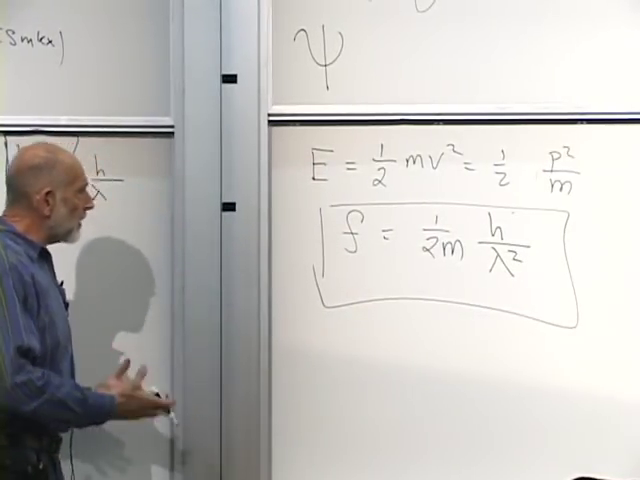
\includegraphics[width=0.64\textwidth]{lecture_02_figure_05.png}
\caption{Đối với một hạt chậm, \(E=p^2/(2m)\) và \(p=h/\lambda\) cho \(f=h/(2m\lambda^2)\).}
\lectureframe{00:37:47}
\end{figure}

Đối với ánh sáng,
\begin{equation}
f\propto\frac{1}{\lambda},
\end{equation}
trong khi đối với vật chất chuyển động chậm,
\begin{equation}
f\propto\frac{1}{\lambda^2}.
\end{equation}
Không cần phải ghi nhớ riêng lẻ hệ thức thứ hai. Luôn có thể dựng lại nó từ \(E=p^2/(2m)\), \(E=hf\) và \(p=h/\lambda\). Đối với một electron chuyển động chậm trong nguyên tử, nó cho tần số của sóng Schr\"odinger tương ứng.

\begin{classroomqa}
\lecturetimestamp{00:38:35}
\audiencequestion{Hệ thức tần số--bước sóng phi tương đối tính có áp dụng cho các hạt khác electron không?}
\lecturerresponse{Có. Nó áp dụng cho mọi hạt chuyển động chậm hơn ánh sáng rất nhiều. Phép nội suy tương đối tính giữa giới hạn chậm và giới hạn ánh sáng là một chủ đề riêng.}
\end{classroomqa}

\begin{classroomqa}
\lecturetimestamp{00:38:55}
\audiencequestion{Quan hệ nào áp dụng cho neutrino?}
\lecturerresponse{Điều đó phụ thuộc vào tốc độ của neutrino. Hầu hết neutrino gặp trong tự nhiên chuyển động rất gần tốc độ ánh sáng, nên quan hệ trong giới hạn ánh sáng là một xấp xỉ tốt. Thay vào đó, một neutrino chuyển động chậm hơn ánh sáng rất nhiều sẽ tuân theo quan hệ phi tương đối tính.}
\end{classroomqa}

\editorialnote{Một trao đổi ngắn với thính giả ngay sau câu hỏi về neutrino bàn về biên độ, lượng tử và sự khác nhau của các bước sóng electron, nhưng câu chữ bị hỏng quá nặng nên không thể phục dựng một cách chắc chắn. Phần trả lời còn khôi phục được đã hoãn việc nêu quan hệ tổng quát giữa biên độ và các lượng tử có bước sóng khác nhau.}

\begin{classroomqa}
\lecturetimestamp{00:39:56}
\audiencequestion{Một electron từ một máy gia tốc \(20\,\mathrm{keV}\) là chậm hay tương đối tính?}
\lecturerresponse{Nó được xem là chậm. Trong hệ đơn vị với \(c=1\), khối lượng, năng lượng và động lượng có thể được biểu diễn bằng cùng một đơn vị. Thang năng lượng nghỉ của electron xấp xỉ \(0.5\,\mathrm{MeV}\), còn \(20\,\mathrm{keV}\) thì nhỏ hơn nhiều. Tương đương, tiêu chuẩn động lượng phi tương đối tính là \(p\ll mc\).}
\end{classroomqa}

Phép so sánh năng lượng trong ví dụ là
\begin{equation}
K=20\,\mathrm{keV}\ll m_ec^2\simeq0.5\,\mathrm{MeV}.
\end{equation}
\editorialnote{Đoạn nguồn tại 00:39:56--00:41:40 đưa vào \(20\,\mathrm{keV}\) như một năng lượng máy gia tốc rồi diễn đạt tiêu chuẩn tương đối tính theo động lượng so với khối lượng nghỉ. Việc viết riêng tiêu chuẩn năng lượng động học và tiêu chuẩn động lượng tránh đồng nhất năng lượng được nêu với một động lượng mà vẫn giữ kết luận phi tương đối tính đã phát biểu.}

\section{Vận tốc pha, vận tốc nhóm và sự tán sắc}

\begin{classroomqa}
\lecturetimestamp{00:41:46}
\audiencequestion{Có thể dùng tích của tần số với bước sóng để suy ra vận tốc của sóng electron không?}
\lecturerresponse{Nó cho vận tốc pha, chứ không phải vận tốc gán cho electron. Một gói định xứ có cả vận tốc pha, mô tả chuyển động của các đỉnh và đáy sóng bên trong nó, lẫn vận tốc nhóm, mô tả chuyển động của đường bao. Vận tốc nhóm được đồng nhất với chuyển động của hạt.}
\end{classroomqa}

Một gói sóng, xét cục bộ, trông như một hàm sin hay cos nhưng bị giới hạn bởi một đường bao. Khi nó chuyển động, đường bao và các đỉnh sóng bên trong không nhất thiết chuyển động cùng tốc độ.\footnote{Hình minh họa này theo sau phần thảo luận về gói sóng tại 00:42:34--00:44:11.}

\begin{figure}[t]
\centering
\begin{tikzpicture}[x=0.75cm,y=0.8cm]
\draw[->] (-0.5,0) -- (12.8,0);
\draw[thick] plot[domain=0:12,samples=140] (\x,{1.10*exp(-0.20*(\x-6)^2)});
\draw[thick] plot[domain=0:12,samples=140] (\x,{-1.10*exp(-0.20*(\x-6)^2)});
\draw[thick] plot[domain=0:12,samples=240] (\x,{1.10*exp(-0.20*(\x-6)^2)*sin(6*\x r)});
\draw[->] (4.1,1.45) -- (7.5,1.45);
\draw (5.8,1.8) node{group motion};
\draw[->] (7.0,-1.55) -- (8.3,-1.55);
\draw (8.7,-1.55) node[right]{phase motion};
\end{tikzpicture}
\caption{Một gói sóng định xứ mà đường bao và pha bên trong nói chung chuyển động với các vận tốc khác nhau.}
\end{figure}

Vận tốc pha là vận tốc của các đỉnh, đáy và các pha cố định khác của một thành phần đơn sắc. Đối với quan hệ tán sắc phi tương đối tính,
\begin{equation}
v_\phi=f\lambda=\frac{h}{2m\lambda}.
\end{equation}
Nó phụ thuộc vào bước sóng. Vì thế các thành phần có bước sóng khác nhau có các vận tốc pha khác nhau, nên các đỉnh sóng có thể đi xuyên qua gói và gói có thể tán ra. Vận tốc nhóm là vận tốc của toàn bộ gói, và đó là vận tốc được đồng nhất với chuyển động của hạt.

Có một trường hợp đặc biệt đơn giản. Nếu tất cả các thành phần bước sóng đều chuyển động với cùng một vận tốc, thì vận tốc pha và vận tốc nhóm trùng nhau. Ánh sáng trong chân không có tính chất này: mọi bước sóng đều truyền với \(c\). Quan hệ cho hạt chậm thì không như vậy; \(f\lambda\) của nó thay đổi theo \(\lambda\).

Phương trình
\begin{equation}
f=\frac{h}{2m\lambda^2}
\end{equation}
là phương trình Schr\"odinger tự do dưới một dạng hơi biến đổi. Tần số xác định sự phụ thuộc theo thời gian của một sóng phẳng, bước sóng xác định sự phụ thuộc theo không gian của nó, và phương trình Schr\"odinger liên hệ hai đại lượng ấy. Ngược lại, thay một sóng có tần số xác định và bước sóng xác định vào phương trình Schr\"odinger tự do sẽ tái tạo quan hệ tán sắc này.

\begin{classroomqa}
\lecturetimestamp{00:47:02}
\audiencequestion{Vận tốc pha có thể vượt quá tốc độ ánh sáng không?}
\lecturerresponse{Có. Vận tốc pha không mang thông tin. Thông tin và gói định xứ truyền với vận tốc nhóm, nên một vận tốc pha siêu quang không cho phép truyền tín hiệu siêu quang.}
\end{classroomqa}

\section{Không gian hữu hạn và động lượng rời rạc}

Mối quan tâm sau cùng là các sóng trong một không gian vô hạn, nhưng một hệ hữu hạn là điểm khởi đầu an toàn hơn. Vô hạn không phải là thứ mà máy tính có thể lưu trữ hay thao tác trực tiếp. Trước hết người ta thiết lập các phương trình cho một hệ hữu hạn rồi chỉ sau đó mới lấy giới hạn trong đó kích thước của nó trở nên lớn tùy ý. Thói quen này hữu ích trong toàn bộ cơ học lượng tử, lý thuyết trường lượng tử và vật lý hạt.

Không mất đi điều gì cốt yếu khi bắt đầu trong một chiều không gian. Sóng có thể tồn tại trên một dây đàn violin, trên một sợi dây đang được rung, hoặc trong một thế giới một chiều trừu tượng. Hệ hữu hạn hiển nhiên nhất là một đoạn có độ dài \(L\) với hai đầu phản xạ. Một sóng truyền đến một đầu, phản xạ và truyền ngược lại. Đó là một điều kiện biên phản xạ hoàn toàn hợp lệ, nhưng có một bất tiện: động lượng không được bảo toàn trong hệ sóng. Một sóng truyền sang phải mang động lượng sang phải; sau phản xạ nó mang động lượng sang trái. Biên đã cung cấp xung lực và hấp thụ phần chênh lệch.

Sự đảo chiều động lượng ở một đầu phản xạ có thể được biểu diễn bằng sơ đồ.\footnote{Hình minh họa này theo sau lập luận về biên phản xạ tại 00:49:24--00:51:08.}

\begin{figure}[t]
\centering
\begin{tikzpicture}[x=1cm,y=1cm]
\draw[thick] (0,0) -- (7,0);
\draw[very thick] (0,-0.45) -- (0,0.45);
\draw[very thick] (7,-0.45) -- (7,0.45);
\draw[->,thick] (1.0,0.35) -- (5.8,0.35) node[midway,above]{\(p>0\)};
\draw[->,thick] (5.8,-0.35) -- (1.0,-0.35) node[midway,below]{\(p<0\)};
\draw (3.5,-0.85) node{\(L\)};
\end{tikzpicture}
\caption{Phản xạ ở hai đầu của một đoạn hữu hạn đảo ngược động lượng của một sóng truyền.}
\end{figure}

Có một cách khác để làm cho hệ trở nên hữu hạn mà vẫn bảo toàn động lượng. Hãy đồng nhất hai đầu mút của đoạn thẳng. Có thể vẽ kết quả thành một đường tròn, nhưng không cần một đường tròn thực sự nhúng trong chiều thứ hai. Phát biểu toán học đơn giản là tọa độ có tính tuần hoàn: sau khi đi một tổng quãng đường \(L\), ta trở lại cùng một điểm.

\begin{figure}[t]
\centering
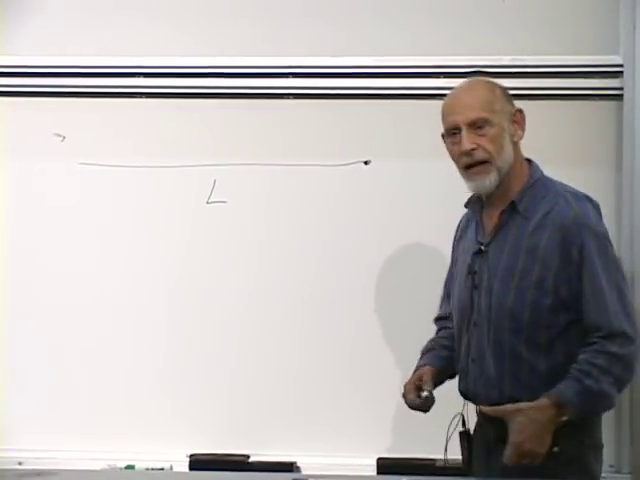
\includegraphics[width=0.72\textwidth]{lecture_02_figure_06.png}
\caption{Một đường đi một chiều có tổng độ dài \(L\) dùng để giới thiệu phép đồng nhất tuần hoàn.}
\lectureframe{00:51:21}
\end{figure}

Việc đồng nhất các đầu mút được biểu thị tường minh trong sơ đồ sau.\footnote{Hình minh họa này theo sau lập luận về phép đồng nhất tuần hoàn tại 00:51:09--00:52:37.}

\begin{figure}[t]
\centering
\begin{tikzpicture}[x=1cm,y=1cm]
\draw[thick] (0,0) -- (7,0);
\fill (0,0) circle (1.5pt);
\fill (7,0) circle (1.5pt);
\draw[->,thick] (1.0,0.35) -- (6.0,0.35);
\draw (3.5,-0.35) node{\(L\)};
\draw[->,bend left=45] (7,0.08) to (0,0.08);
\draw (3.5,1.2) node{identified endpoints};
\end{tikzpicture}
\caption{Không gian một chiều tuần hoàn được tạo thành bằng cách đồng nhất các đầu mút của một đường đi có độ dài \(L\).}
\end{figure}

Khi đó, một sóng chuyển động sang phải sẽ đến đầu mút được vẽ ra, xuất hiện trở lại ở điểm đầu và tiếp tục chuyển động sang phải. Tương tự, một sóng chuyển động sang trái cũng tiếp tục chuyển động sang trái. Không có đầu mút đặc biệt nào nơi sóng bị phản xạ, nên động lượng không đảo chiều. Không gian tuần hoàn làm thể tích trở nên hữu hạn và bảo toàn động lượng, nhưng nó có một hệ quả quan trọng: các động lượng cho phép là rời rạc.

Một số nguyên bước sóng phải vừa khít trong tổng độ dài. Đối với một mode không hằng,
\begin{equation}
\lambda_{|N|}=\frac{L}{|N|},
\qquad |N|=1,2,3,\ldots .
\end{equation}
Do đó độ lớn bước sóng có thể là \(L\), \(L/2\), \(L/3\), vân vân. Một lựa chọn như \(L/\sqrt{2}\) thì không khớp: sau một vòng, sóng sẽ trở về với sai pha và không trùng với giá trị ban đầu của nó.

Dùng \(p=h/\lambda\), độ lớn của động lượng đối với mode không hằng thứ \(|N|\) là
\begin{equation}
|p_N|=\frac{|N|h}{L}.
\end{equation}
Để bao gồm cả hai hướng và mode hằng mà không mơ hồ, tiện nhất là cho nhãn mode mang dấu:
\begin{equation}
p_N=\frac{Nh}{L},
\qquad N=0,\pm1,\pm2,\ldots .
\end{equation}
Các \(N\) dương và âm mô tả các hướng truyền ngược nhau. Mode \(N=0\) là hằng và có động lượng bằng không; nó không có bước sóng hữu hạn để thế vào \(h/\lambda\). Vì vậy khoảng cách động lượng cơ bản là \(h/L\).

Đối với một \(L\) vĩ mô, cả \(h\) lẫn \(1/L\) đều làm cho khoảng cách này cực nhỏ, nên các giá trị cho phép tạo thành một tập rất dày và trông gần như liên tục. Tuy vậy, một hạt cườm bị ràng buộc trên một vòng dây tròn vẫn có đúng phổ rời rạc như thế.

\begin{classroomqa}
\lecturetimestamp{00:58:27}
\audiencequestion{Đại lượng bị lượng tử hóa là tổng động lượng của sóng, hay động lượng gắn với một chu kỳ?}
\lecturerresponse{Phát biểu này áp dụng cho động lượng của mỗi lượng tử. Mỗi lượng tử có một trong các động lượng rời rạc cho phép. Do đó tổng động lượng của bất kỳ tập hợp lượng tử nào cũng là một bội số nguyên của đơn vị cơ bản \(h/L\).}
\end{classroomqa}

\begin{classroomqa}
\lecturetimestamp{00:59:22}
\audiencequestion{Vì sao sóng phải trở về cùng một giá trị sau một vòng?}
\lecturerresponse{Các đầu mút đã được đồng nhất là cùng một điểm vật lý, nên một trường quan sát được phải có cùng giá trị tại đó. Một sự không khớp sẽ đòi hỏi một bước nhảy đột ngột của trường tại điểm ấy. Sự gián đoạn như vậy là tốn kém về năng lượng và động lượng; các cấu hình trường chấp nhận được là liên tục và tuần hoàn.}
\end{classroomqa}

\begin{classroomqa}
\lecturetimestamp{01:00:09}
\audiencequestion{Điều gì xảy ra nếu sóng được định xứ thành một gói?}
\lecturerresponse{Một gói là một tổng Fourier của các sóng phẳng, hay tương đương là của các hàm sin và cos. Trong không gian tuần hoàn, tổng đó chỉ có thể chứa các mode động lượng rời rạc cho phép. Vì vậy, phát biểu về lượng tử hóa là một phát biểu về các thành phần Fourier của mọi gói chấp nhận được.}
\end{classroomqa}

\begin{classroomqa}
\lecturetimestamp{01:01:01}
\audiencequestion{Có vấn đề gì không nếu độ dài tuần hoàn \(L\) trở nên cực nhỏ?}
\lecturerresponse{Khi \(L\) giảm, động lượng cơ bản \(h/L\) trở nên rất lớn. Điều đó không hàm ý một mâu thuẫn trực tiếp nào ở các độ dài vi mô thông thường, nhưng việc cố đẩy cấu trúc này đến chế độ độ dài Planck được kỳ vọng sẽ đòi hỏi vật lý mới.}
\end{classroomqa}

Giờ hãy hiểu bức tranh đường tròn theo nghĩa đen: một hạt cườm chuyển động trên một vòng dây tròn bán kính \(r\), có chu vi \(L=2\pi r\). Các động lượng tiếp tuyến cho phép của nó là
\begin{equation}
p_N=\frac{Nh}{2\pi r}=\frac{N\hbar}{r}.
\end{equation}
Đối với một hạt phi tương đối tính trên quỹ đạo tròn, mômen động lượng là \(mvr\). Vì \(p=mv\) trong chế độ đó, đại lượng này là \(rp\). Biểu thức \(mvr\) không có tính tổng quát tương đối tính, vì khi đó \(p\) không còn đơn giản là \(mv\), nhưng động lượng nhân với khoảng cách vuông góc vẫn là quan hệ đúng. Dưới dạng vectơ,\footnote{Bài giảng lúc đầu dùng \(L\) cho mômen động lượng, rồi nhận ra sự xung đột của nó với \(L\) cho độ dài tuần hoàn và đổi ký hiệu. Ở đây dùng \(J\) xuyên suốt; xem 01:03:40--01:05:21.}
\begin{equation}
\vec J=\vec r\times\vec p,
\end{equation}
và đối với chuyển động tròn theo tiếp tuyến, độ lớn của nó là \(J=rp\). Do đó
\begin{equation}
J_N=rp_N=N\hbar.
\end{equation}
Độ giãn cách của động lượng tuyến tính phụ thuộc vào kích thước của đường tròn, còn đơn vị mômen động lượng thì luôn là \(\hbar\). Có những ngoại lệ đối với quy tắc số nguyên khi có fermion; các ngoại lệ đó sẽ được để lại bàn sau.

Nhiệm vụ tiếp theo là kết nối các trường với các hạt và lượng tử một cách chính xác hơn. Điều đó đòi hỏi quay lại ngắn gọn với cơ học lượng tử của các toán tử và dao động tử điều hòa.

\section{Các mode sóng và các toán tử lượng tử}

Phần cơ học lượng tử tiếp theo tất yếu có tính trừu tượng và nhằm mục đích ôn lại. Dao động tử điều hòa là hệ cốt yếu vì sóng là một dao động. Tại một điểm cố định, điện trường, từ trường hay bất kỳ biên độ sóng nào khác đều biến thiên tuần hoàn theo thời gian; nói rằng một thành phần có tần số tức là đã nói rằng nó dao động.

Một sóng tổng quát không nhất thiết chỉ có một bước sóng. Ánh sáng gồm nhiều màu có thể trộn lẫn với nhau, và ngược lại, một lăng kính có thể tách ánh sáng hỗn hợp thành các màu thành phần của nó, như trong phép phân tích ánh sáng trắng của Newton. Mỗi thành phần có bước sóng, tần số, biên độ, năng lượng và động lượng riêng. Vì thế sóng hỗn hợp có thể được phân giải thành các lượng tử có năng lượng và động lượng khác nhau. Mỗi bước sóng xác định một tần số, và mỗi thành phần có tần số xác định hành xử như một dao động tử. Đó là lý do vì sao dao động tử điều hòa, chứ không phải một hệ lượng tử tùy ý, là khối cấu thành tự nhiên của một trường.

Các đại lượng quan sát được trong cơ học lượng tử được biểu diễn bởi các toán tử. Các toán tử có thể được cộng và nhân, nhưng khác với các số thông thường, tích của chúng không nhất thiết độc lập với thứ tự. Gọi \(A\) và \(B\) biểu diễn hai tính chất của một hệ, mỗi tính chất đều có thể đo được riêng rẽ. Chẳng hạn, \(A\) có thể biểu diễn điện trường và \(B\) một từ trường. Nếu các giá trị đo được là các số thông thường \(a\) và \(b\), thì
\begin{equation}
ab=ba.
\end{equation}
Tích bằng số của chúng không thể phụ thuộc vào thứ tự nhân. Tuy nhiên, trong cơ học lượng tử, các toán tử tương ứng thay vào đó có thể thỏa mãn \(AB-BA\neq0\).

Thoạt đầu điều này có vẻ vô nghĩa. Nếu phép đo điện trường cho ra một số và phép đo từ trường cho ra một số khác, thì nhân hai số đó theo thứ tự nào cũng phải cho cùng một kết quả. Cách tháo gỡ là: khi các tích toán tử phụ thuộc vào thứ tự, thì hai đại lượng ấy không thể được đo đồng thời. Thí nghiệm đo một đại lượng gây nhiễu cho phép đo đại lượng kia. Không có mâu thuẫn nào, vì hai giá trị số ấy không thể thu được cùng nhau.

Khi hai đại lượng có thể được đo đồng thời, các giá trị đo được của chúng là các số thông thường, và các số đó giao hoán. Vì vậy, phép kiểm tra tính đo đồng thời là giao hoán tử
\begin{equation}
[A,B]=AB-BA.
\end{equation}
Một giao hoán tử triệt tiêu có nghĩa là các đại lượng quan sát được là tương hợp; một giao hoán tử khác không có nghĩa là các phép đo tương ứng gây nhiễu lẫn nhau. Đảo thứ tự hai mục thì đảo dấu:
\begin{equation}
[B,A]=-[A,B].
\end{equation}

Đối với một hạt phi tương đối tính, ba thành phần vị trí giao hoán với nhau, và ba thành phần động lượng cũng vậy:
\begin{align}
[x,y]&=[y,z]=[z,x]=0,\\
[p_x,p_y]&=[p_y,p_z]=[p_z,p_x]=0.
\end{align}
Cả ba tọa độ có thể được xác định cùng nhau, và cả ba thành phần động lượng cũng có thể được xác định cùng nhau. Các thành phần vị trí và động lượng tương ứng không giao hoán:
\begin{equation}
[x,p_x]=[y,p_y]=[z,p_z]=i\hbar,
\end{equation}
trong khi các thành phần trộn như \([x,p_y]\) thì triệt tiêu. Việc đo một tọa độ vị trí gây cho hạt một nhiễu động ở động lượng liên hợp. Tương đương, tích của độ bất định vị trí và động lượng tương ứng được chi phối bởi \(\hbar\).

\begin{classroomqa}
\lecturetimestamp{01:16:30}
\audiencequestion{Khi chuyển từ \(x\) sang \(y\), liệu \(i\) trong giao hoán tử có nên đổi thành \(j\) không?}
\lecturerresponse{Không. Ký hiệu \(i\) luôn luôn là đơn vị ảo, căn bậc hai của âm một. Nó không phải là nhãn vectơ đơn vị Đề-các, cũng không phải một trong các ký hiệu quaternion \(i,j,k\).}
\end{classroomqa}

\begin{classroomqa}
\lecturetimestamp{01:17:24}
\audiencequestion{Có phải \(AB-BA\) có nghĩa là đo \(A\) trước rồi đến \(B\), rồi sau đó đảo ngược thứ tự đo không?}
\lecturerresponse{Không. Hai hạng đó là các tích toán tử hoặc ma trận theo hai thứ tự đại số khác nhau. Chúng không biểu thị một chuỗi phép đo theo nghĩa đen. Mối liên hệ với các phép đo không tương hợp là hệ quả của đại số toán tử, chứ không phải định nghĩa của phép nhân.}
\end{classroomqa}

\begin{classroomqa}
\lecturetimestamp{01:18:32}
\audiencequestion{Các giao hoán tử vị trí--động lượng này có áp dụng trực tiếp cho một photon không?}
\lecturerresponse{Không trực tiếp. Chúng áp dụng gọn gàng cho các hạt phi tương đối tính. Vị trí của photon khó định nghĩa hơn, nên mệnh đề tương tự đòi hỏi phải thận trọng hơn và không cần đến ở đây.}
\end{classroomqa}

\section{Dao động tử điều hòa lượng tử}

Quả nặng gắn trên lò xo, sóng âm và sóng ánh sáng đều cho các ví dụ về chuyển động dao động. Mọi dao động tử điều hòa lý tưởng đều có một tần số. Đối với lò xo, một chu kỳ trọn vẹn không chỉ đơn thuần là thời gian cần để quả nặng trở lại cùng vị trí; nó còn phải trở lại vị trí ấy với chuyển động theo cùng một chiều. Số chu kỳ hoàn chỉnh trong mỗi giây là \(f\), và \(\omega=2\pi f\).

Theo cơ học cổ điển, một dao động tử lý tưởng có thể có bất kỳ năng lượng không âm nào. Một cú đẩy nhẹ cho một năng lượng nhỏ, còn một cú đẩy mạnh hơn cho một năng lượng lớn hơn. Một lò xo thật cuối cùng sẽ gãy hoặc nóng chảy, nhưng sự lý tưởng hóa toán học có một dải liên tục các năng lượng dương. Dao động tử lượng tử thì khác: các năng lượng được phép của nó tạo thành một thang rời rạc với khoảng cách đều nhau. Chọn gốc năng lượng sao cho mức thấp nhất được gọi là 0,
\begin{equation}
E_n=n\hbar\omega,
\qquad n=0,1,2,\ldots .
\end{equation}
Các mức cách đều có thể được hình dung như sau.\footnote{Sơ đồ mức năng lượng này bám theo phần thảo luận trên bảng tại 01:21:20--01:23:56.}

\begin{figure}[t]
\centering
\begin{tikzpicture}[x=1cm,y=0.9cm]
\draw[->] (0,0) -- (0,5.35);
\draw (0,5.5) node[above]{energy};
\foreach \y/\lab in {0.6/{0},1.6/{\hbar\omega},2.6/{2\hbar\omega},3.6/{3\hbar\omega},4.6/{n\hbar\omega}}
{
  \draw[thick] (0.2,\y) -- (2.2,\y);
  \draw (-0.25,\y) node[left]{\(\lab\)};
}
\draw[->,thick] (2.8,0.68) -- (2.8,1.52);
\draw (3.2,1.1) node[right]{\(a_+\)};
\draw[->,thick] (3.7,1.52) -- (3.7,0.68);
\draw (4.1,1.1) node[right]{\(a_-\)};
\end{tikzpicture}
\caption{Các mức của dao động tử cách đều theo quy ước \(E_n=n\hbar\omega\).}
\end{figure}

Khoảng cách \(\hbar\omega\) chính là năng lượng đã được gán trước đó cho một photon có tần số góc \(\omega\). Giá trị \(2\hbar\omega\) có thể là năng lượng của một lượng tử thuộc về một dao động tử có tần số \(2\omega\), hoặc là năng lượng của hai lượng tử trong một dao động tử có tần số \(\omega\). Cách hiểu thứ hai là cách cần dùng ở đây. Một dao động tử đơn lẻ có tần số cố định có thể chứa 0, 1, 2, 3 hoặc nhiều lượng tử hơn, và không có mức năng lượng được phép nào nằm giữa các nấc.

Số nguyên \(n\) gắn nhãn cho trạng thái của dao động tử, được viết dưới dạng ket \(|n\rangle\). Trạng thái \(|0\rangle\) là trạng thái cơ bản, \(|1\rangle\) có một lượng tử kích thích, \(|2\rangle\) có hai, v.v. Ket đơn giản chỉ là ký hiệu cho trạng thái mà các toán tử tác dụng lên.

Định nghĩa toán tử nâng \(a_+\) đưa một trạng thái lên một mức và toán tử hạ \(a_-\) đưa nó xuống một mức:
\begin{align}
a_+|n\rangle &= \sqrt{n+1}\,|n+1\rangle,\\
a_-|n\rangle &= \sqrt{n}\,|n-1\rangle.
\end{align}
Các hệ số căn bậc hai bằng số là một phần của các định nghĩa. Trên trạng thái thấp nhất,
\begin{equation}
a_-|0\rangle=0,
\end{equation}
vì không có trạng thái nào nằm dưới trạng thái cơ bản.

Điều quan trọng ở đây là phải phân biệt các số thông thường với các toán tử. Nhãn \(n\) và các hệ số như \(\sqrt n\) là các số thông thường; chúng giao hoán với mọi thứ. Các ký hiệu \(a_+\) và \(a_-\) là các toán tử, và thứ tự của chúng phải được giữ nguyên.

Trước hết hạ \(|n\rangle\) xuống, rồi nâng nó trở lại. Bước hạ cho
\begin{equation}
a_-|n\rangle=\sqrt n\,|n-1\rangle.
\end{equation}
Tác dụng \(a_+\) lên trạng thái thu được đưa vào thêm một hệ số \(\sqrt n\), vì việc nâng \(|n-1\rangle\) đưa nó trở lại \(|n\rangle\):
\begin{align}
a_+a_-|n\rangle
&=a_+\bigl(\sqrt n\,|n-1\rangle\bigr)\\
&=\sqrt n\,\sqrt n\,|n\rangle\\
&=n|n\rangle.
\end{align}
Do đó \(a_+a_-\) cho biết số mức. Chẳng hạn, giả sử \(|\chi\rangle\) được biết là một trạng thái riêng của toán tử số nhưng nhãn mức của nó chưa biết. Nếu
\begin{equation}
a_+a_-|\chi\rangle=q|\chi\rangle,
\end{equation}
thì hệ số bằng số thông thường \(q\) là số lượng tử trong trạng thái đó. Vì vậy tích ấy là toán tử số,
\begin{equation}
\hat n=a_+a_-,
\end{equation}
và, theo quy ước năng lượng đã chọn, Hamiltonian là
\begin{equation}
H=\hbar\omega\,a_+a_-.
\end{equation}
Thật vậy, tác dụng lên bất kỳ mức nào cũng cho \(H|n\rangle=n\hbar\omega|n\rangle\).

Bây giờ đảo ngược thứ tự. Nâng trước cho \(\sqrt{n+1}|n+1\rangle\). Sau đó hạ xuống thì quay về \(|n\rangle\) và đưa ra hệ số thứ hai \(\sqrt{n+1}\):
\begin{align}
a_-a_+|n\rangle
&=a_-\bigl(\sqrt{n+1}\,|n+1\rangle\bigr)\\
&=\sqrt{n+1}\,\sqrt{n+1}\,|n\rangle\\
&=(n+1)|n\rangle.
\end{align}
Hai thứ tự ấy khác nhau một đơn vị trên mọi trạng thái, nên
\begin{equation}
[a_-,a_+]=a_-a_+-a_+a_-=1.
\end{equation}

Dao động tử còn có biên độ và pha. Pha của nó cho biết nó đang ở đâu trong chu trình; cụ thể, có thể cố định pha bằng thời điểm mà dao động tử đi qua gốc theo một chiều đã chọn. Việc làm trễ lần đi qua đó làm đổi pha mà không làm đổi tần số. Các toán tử bậc thang kết hợp các biến lượng tử gắn với biên độ và pha. Đại số của chúng vốn dĩ là lượng tử, nhưng tác dụng của chúng thì đơn giản: \(a_+\) thêm một lượng tử năng lượng của dao động tử và \(a_-\) lấy đi một lượng tử. Đối với một mode điện từ, các lượng tử đó là photon, nên hai toán tử này được gọi là toán tử tạo và toán tử hủy.

\begin{classroomqa}
\lecturetimestamp{01:37:34}
\audiencequestion{Các toán tử nâng và hạ có tương ứng với một phép đo vật lý không?}
\lecturerresponse{Số photon thì đo được. Các toán tử \(a_+\) và \(a_-\) tự chúng không phải là các đại lượng quan sát được có thể đo riêng rẽ, vì những lý do kỹ thuật bổ sung. Giao hoán tử của chúng cho thấy hai toán tử đó không giao hoán, nhưng riêng sự kiện ấy tự nó không phải là lập luận cho thấy từng toán tử một, xét riêng lẻ, là không quan sát được.}
\end{classroomqa}

Một tập hợp các lò xo với các tần số riêng khác nhau cho ta nhiều dao động tử độc lập. Các mode điện từ của một hốc cộng hưởng cũng vậy: một bước sóng có thể được kích thích mà không buộc những bước sóng khác phải có cùng mức kích thích. Về mặt lượng tử, các toán tử tạo và hủy thêm vào và lấy đi các lượng tử có tần số cố định trong từng dao động tử độc lập. Ngôn ngữ này là then chốt vì các hạt sẽ được đồng nhất chính với những lượng tử đó.

\section{Một trường như một tập hợp các dao động tử}

Quay lại không gian một chiều tuần hoàn có tổng chiều dài \(L\). Các mode không hằng của nó có độ lớn bước sóng
\begin{equation}
\lambda_N=\frac{L}{N},
\qquad N=1,2,3,\ldots ,
\end{equation}
và các tần số góc không âm tương ứng \(\omega_N\). Để so sánh với phổ động lượng đã nêu trước đó, sẽ hữu ích nếu đổi nhãn số nguyên có dấu thành \(M\):
\begin{equation}
p_M=\frac{Mh}{L},
\qquad M=0,\pm1,\pm2,\ldots .
\end{equation}
Dấu của \(M\) ghi lại hướng truyền.
\editorialnote{Trong khoảng 01:42:08--01:42:24, chỉ số mode theo tần số được sửa từ một dải có dấu thành một dải chạy từ 0 trở lên. Ký hiệu \(M\) ở đây chỉ được dùng để tách biệt ký hiệu động lượng có dấu khỏi nhãn mode theo tần số không âm \(N\); nó không đưa vào các số chiếm đóng độc lập cho \(+M\) và \(-M\). Danh sách các dao động tử không hằng bắt đầu tại \(N=1\).}

Mỗi tần số được phép hành xử như một dao động tử điều hòa. Năng lượng có thể được thêm một cách độc lập vào tần số này rồi vào tần số khác. Ví dụ chi tiết đầu tiên về một trường lượng tử được để sang bài giảng tiếp theo, nhưng ký hiệu trạng thái thì đã rõ. Sắp các mode không hằng theo thứ tự từ bước sóng dài nhất trở đi, ta viết
\begin{equation}
|n_1,n_2,n_3,\ldots\rangle,
\end{equation}
trong đó \(n_N=0,1,2,\ldots\) là số lượng tử trong dao động tử có tần số \(\omega_N\). Thành phần thứ nhất cho biết có bao nhiêu lượng tử chiếm mode có bước sóng dài nhất, thành phần thứ hai cho biết có bao nhiêu lượng tử chiếm mode kế tiếp, và cứ thế mãi không dứt.

Các họa âm của một sợi dây làm cho cách xây dựng này trở nên cụ thể. Sự chuyển tiếp từ mode cơ bản qua hai họa âm tiếp theo được biểu diễn bằng sơ đồ.\footnote{Sơ đồ này bám theo phần thảo luận về các họa âm của dây tại 01:45:20--01:47:46.}

\begin{figure}[t]
\centering
\resizebox{\linewidth}{!}{%
\begin{tikzpicture}[x=0.98cm,y=1cm]
\draw[gray] (0,2.5) -- (6,2.5);
\draw[thick] plot[domain=0:6,samples=120] (\x,{2.5+0.48*sin(30*\x)});
\fill (0,2.5) circle (1.4pt);
\fill (6,2.5) circle (1.4pt);
\node[right] at (6.25,2.5) {fundamental: \(\omega_1\)};

\draw[gray] (0,1.25) -- (6,1.25);
\draw[thick] plot[domain=0:6,samples=120] (\x,{1.25+0.42*sin(60*\x)});
\fill (0,1.25) circle (1.4pt);
\fill (3,1.25) circle (1.4pt);
\fill (6,1.25) circle (1.4pt);
\node[right] at (6.25,1.25) {second harmonic: \(2\omega_1\)};

\draw[gray] (0,0) -- (6,0);
\draw[thick] plot[domain=0:6,samples=120] (\x,{0.42*sin(90*\x)});
\fill (0,0) circle (1.4pt);
\fill (2,0) circle (1.4pt);
\fill (4,0) circle (1.4pt);
\fill (6,0) circle (1.4pt);
\node[right] at (6.25,0) {third harmonic: \(3\omega_1\)};
\end{tikzpicture}%
}
\caption{Mode cơ bản của dây và họa âm thứ hai, thứ ba của nó, với 0, 1 và 2 nút bên trong.}
\end{figure}

Mode cơ bản dao động như một vòm rộng duy nhất và không có nút bên trong. Nó là một dao động tử, và nó có thể chứa \(n_1=0,1,2,\ldots\) lượng tử; mỗi kích thích cần \(\hbar\omega_1\). Họa âm thứ hai có một nút bên trong và tần số gấp đôi. Nếu mode cơ bản phát ra nốt đô trung, thì mode này phát ra nốt đô cao hơn một quãng tám. Nó có một số chiếm đóng độc lập \(n_2\), và mỗi lượng tử của nó cần \(\hbar\omega_2=2\hbar\omega_1\). Họa âm thứ ba có hai nút bên trong và tần số gấp 3 lần tần số cơ bản. Nó có số chiếm đóng độc lập riêng \(n_3\), và số này một lần nữa có thể là bất kỳ số nguyên không âm nào.

Xét từng mode, theo quy ước năng lượng dùng ở trên, năng lượng bằng số chiếm đóng nhân với năng lượng lượng tử. Gộp các đóng góp đó lại, ta được
\begin{equation}
E=\sum_{N=1}^{\infty} n_N\hbar\omega_N.
\end{equation}
\editorialnote{Tổng được viết tường minh này là sự gom góp đại số của các năng lượng mode đã được phát biểu riêng rẽ tại 01:44:02--01:47:46.}

Cùng một toán học của dao động tử điều hòa phải được lặp lại cho mọi mode của trường, với một toán tử tạo và một toán tử hủy cho mỗi dao động tử độc lập. Trong bức tranh sơ cấp đầu tiên này, một trường lượng tử chính là toàn bộ tập hợp ấy của các dao động tử và đại số tạo--hủy của chúng.

Ngôn ngữ này được điều chỉnh cho phù hợp với tán xạ hạt. Các lượng tử có năng lượng và xung lượng xác định đi vào một thí nghiệm, và các lượng tử có những năng lượng và xung lượng khác đi ra khỏi thí nghiệm ấy. Các hạt ban đầu được loại bỏ bởi các toán tử hủy; các hạt đi ra được đưa vào trạng thái cuối bởi các toán tử tạo ứng với các mode thích hợp.

\begin{classroomqa}
\lecturetimestamp{01:49:38}
\audiencequestion{Có phải cùng một số nguyên đang được dùng để gán nhãn mode dao động và để đếm số lượng tử trong đó không?}
\lecturerresponse{Có hai số nguyên riêng biệt. Nhãn mode \(N\) xác định dạng phân bố trong không gian; trong ví dụ về dây, số nút của nó quyết định tần số \(\omega_N\). Số chiếm chỗ \(n_N\) cho biết có bao nhiêu lượng tử có tần số đó.}
\end{classroomqa}

\chapter{Từ các mode động lượng đến các trường lượng tử cục bộ}

Trường lượng tử là gì, và nó liên hệ với các hạt như thế nào? Công cụ toán học cơ bản là dao động tử điều hòa. Một trường chứa nhiều mode dao động khả dĩ, và việc lượng tử hóa trường tương đương với việc ghép một dao động tử điều hòa lượng tử cho mỗi mode. Cách xây dựng này dễ thấy nhất nếu trước tiên xét một không gian tuần hoàn hữu hạn, nơi các mode được phép tạo thành một danh sách rời rạc.

\section{Không gian tuần hoàn và các số sóng được phép}

Lấy một tọa độ không gian \(x\) và đồng nhất các điểm cách nhau một khoảng \(L\). Có thể hình dung không gian này như một đường tròn có chu vi \(L\). Đây là một thủ pháp thể tích hữu hạn hữu ích. Trên một khoảng hữu hạn có các đầu mút, một sóng truyền sẽ phản xạ ở các đầu. Trên một khoảng tuần hoàn, nó có thể tiếp tục theo một trong hai hướng mà không phản xạ. Đối xứng tịnh tiến, và vì thế là bảo toàn động lượng, được giữ lại trong khi những phức tạp của thể tích vô hạn được tạm thời loại bỏ.

Một sóng phẳng có dạng
\begin{equation}
e^{ikx}.
\end{equation}
Sau một vòng đi quanh đường tròn, nó phải trở về giá trị ban đầu. Vì sóng bằng \(1\) tại \(x=0\), tính tuần hoàn đòi hỏi
\begin{equation}
e^{ikL}=1.
\end{equation}
Vì sao một bội nguyên của \(2\pi\) lại thỏa mãn điều kiện này? Công thức Euler cho
\begin{align}
e^{i2\pi n}
&=\cos(2\pi n)+i\sin(2\pi n)\\
&=1,
\qquad n\in\mathbb Z.
\end{align}
Cosin bằng \(1\) và sin bằng \(0\) sau bất kỳ số nguyên chu kỳ nào. Do đó,
\begin{equation}
kL=2\pi n,
\qquad
k=\frac{2\pi n}{L},
\qquad n\in\mathbb Z.
\end{equation}
Đại lượng \(k\) là số sóng. Số nguyên \(n\) gắn nhãn một số sóng được phép; nó chưa dùng để đếm hạt.

Cùng điều kiện ấy cũng có thể được biểu diễn theo bước sóng. Bước sóng là khoảng cách mà trên đó pha tăng thêm một chu kỳ trọn vẹn, do đó
\begin{equation}
k\lambda=2\pi,
\qquad
k=\frac{2\pi}{\lambda}.
\end{equation}
Bước sóng dài thì có số sóng nhỏ, còn bước sóng ngắn thì có số sóng lớn. Điều kiện tuần hoàn nói rằng có một số nguyên bước sóng vừa khít quanh đường tròn.

Đối với một sóng cơ học lượng tử, động lượng là
\begin{equation}
p=\frac{h}{\lambda}
=\frac{2\pi\hbar}{\lambda}
=\hbar k.
\end{equation}
Do đó \(k\) và \(p\) chỉ khác nhau bởi hệ số \(\hbar\). \(k\) dương và âm mô tả các sóng chuyển động theo hai hướng đối nhau và các hạt có động lượng ngược hướng. Trong các đơn vị với \(\hbar=1\), người ta thường gọi \(k\) là động lượng mà không phân biệt thêm.

Với mỗi \(k\) được phép, có thể có một số lượng tử nào đó trong mode ấy. Điều này đưa vào một số nguyên thứ hai:
\begin{equation}
n(k)=\text{number of quanta with wave number }k.
\end{equation}
Nó được gọi là số chiếm đóng. Số nguyên trong \(k=2\pi n/L\) gắn nhãn mode; \(n(k)\) cho biết có bao nhiêu hạt chiếm mode đó. Phải cho các số chiếm đóng cho cả \(k\) âm lẫn dương.

\begin{classroomqa}
\lecturetimestamp{00:11:58}
\audiencequestion{Bản thân \(k\) có phải là một số nguyên không?}
\lecturerresponse{Không. Số sóng là một bội nguyên của \(2\pi/L\): \(k=2\pi n/L\). Số nguyên \(n\) trong công thức đó gắn nhãn động lượng được phép, và nó khác với số chiếm đóng \(n(k)\), là số đếm các lượng tử trong mode.}
\end{classroomqa}

\section{Các trạng thái số chiếm đóng và các toán tử mode}

Một trạng thái lượng tử là một vectơ, hay phần tử tuyến tính. Các vectơ trạng thái có thể được cộng với nhau và nhân với các số, còn các toán tử tác động lên chúng để tạo ra các vectơ trạng thái khác. Các đại lượng thực quan sát được được biểu diễn bởi các toán tử Hermite. Những sự kiện sơ đẳng này quan trọng ở đây vì cả trạng thái nhiều hạt lẫn trường đều sẽ được xây dựng từ các tổ hợp tuyến tính và các toán tử.

Đặt
\begin{equation}
k_j=\frac{2\pi j}{L},
\qquad j\in\mathbb Z.
\end{equation}
Một nhãn thuận tiện cho một trạng thái nhiều hạt là toàn bộ dãy số chiếm đóng. Dùng ký hiệu tắt \(n_j\equiv n(k_j)\) cho các phần tử đã hiển thị, viết
\begin{equation}
\big|\{n(k_j)\}\big\rangle
=
\big|\ldots,n_{-2},n_{-1},n_0,n_1,n_2,\ldots\big\rangle.
\end{equation}
Phần tử \(n(k_1)\) là số hạt trong mode động lượng dương thứ nhất, \(n(k_2)\) là số trong mode thứ hai, v.v. Dãy này kéo dài vô hạn về cả hai phía.

\begin{figure}[t]
\centering
\includegraphics[width=0.72\textwidth]{lecture_03_figure_02.png}
\caption{Số chiếm đóng \(n(k)\) cho một mode động lượng được phép.}
\lectureframe{00:15:04}
\end{figure}

Mỗi mode động lượng là một dao động điều hòa. Vì vậy nó có một toán tử nâng và một toán tử hạ. Ký hiệu ban đầu viết là \(a^{+}(k)\) và \(a^{-}(k)\) sẽ được viết là \(a^\dagger(k)\) và \(a(k)\). Tác dụng của chúng là
\begin{align}
a^\dagger(k)\big|\ldots,n(k),\ldots\big\rangle
&=
\sqrt{n(k)+1}\notag\\
&\quad{}\times
\big|\ldots,n(k)+1,\ldots\big\rangle,
\\
a(k)\big|\ldots,n(k),\ldots\big\rangle
&=
\sqrt{n(k)}\,
\big|\ldots,n(k)-1,\ldots\big\rangle.
\end{align}
Toán tử \(a^\dagger(k)\) tác động vào ô tương ứng với \(k\), tăng số chiếm đóng ở đó lên một đơn vị, và nhân trạng thái với \(\sqrt{n(k)+1}\). Toán tử \(a(k)\) làm giảm chính ô đó và đưa vào hệ số \(\sqrt{n(k)}\). Có một cặp như vậy cho mỗi động lượng được phép.

\begin{figure}[t]
\centering
\includegraphics[width=0.58\textwidth]{lecture_03_figure_03.png}
\caption{Các toán tử tạo và hủy gắn với mode động lượng \(k\).}
\lectureframe{00:17:14}
\end{figure}

\section{Các hệ số Fourier trở thành toán tử}

Mối liên hệ giữa các toán tử dao động tử này với một trường bắt đầu từ một chuỗi Fourier cổ điển thông thường. Một trường cổ điển phức trên khoảng tuần hoàn có thể được viết
\begin{align}
\psi(x)&=\sum_k \alpha(k)e^{ikx},\\
\psi^*(x)&=\sum_k \alpha^*(k)e^{-ikx},
\end{align}
trong đó mọi tổng đều lấy trên các giá trị được phép \(k=2\pi n/L\). Điều này tương đương với việc khai triển trường theo sin và cos.

Trường phức có một phần thực và một phần ảo. Liên hợp phức của nó đảo dấu phần ảo, và \(e^{ikx}\) trở thành \(e^{-ikx}\). Chỉ rõ tất cả các hệ số \(\alpha(k)\) là chỉ rõ trường cổ điển. Không cần chỉ rõ \(\alpha^*(k)\) một cách độc lập một khi đã biết \(\alpha(k)\), nhưng phần thực và phần ảo của mỗi hệ số là những đại lượng thực riêng biệt. Chúng có thể được đo như các biên độ của những thành phần Fourier tương ứng. Theo nghĩa này, một hệ số phức gói gọn hai đại lượng quan sát cổ điển.

Việc lượng tử hóa thay các hệ số Fourier cổ điển này bằng các toán tử. Một dấu bằng thông thường sẽ đồng nhất các đối tượng thuộc những loại khác nhau, nên tốt hơn là viết một quy tắc thay thế:
\begin{equation}
\alpha(k)\rightsquigarrow a(k),
\qquad
\alpha^*(k)\rightsquigarrow a^\dagger(k).
\end{equation}
Với một lựa chọn nhất quán về dấu Fourier, các trường lượng tử được định nghĩa bởi
\begin{align}
\Psi(x)&=\sum_k a(k)e^{ikx},\\
\Psi^\dagger(x)&=\sum_k a^\dagger(k)e^{-ikx}.
\end{align}
\editorialnote{Phần thảo luận bằng lời có thay đổi và về sau có đặt lại vấn đề về quy ước dấu Fourier. Cặp liên hợp dùng ở đây là quy ước thể hiện trong khai triển trường rõ ràng hơn và trong phép tính trạng thái vị trí: \(\Psi\) đi với \(e^{ikx}\) và \(\Psi^\dagger\) đi với \(e^{-ikx}\). Nếu đảo nhất quán mọi dấu thì ta vẫn mô tả cùng một cách xây dựng.}

Tạm thời, đây là một định nghĩa: trường lượng tử là một tổng Fourier mà các hệ số của nó là các toán tử. Một sự biện minh đầy đủ hơn sẽ phải chỉ ra các toán tử này tái tạo các hệ số cổ điển như thế nào trong một giới hạn thích hợp, điều này đòi hỏi một số động lực học. Câu hỏi đó được hoãn lại. Điều đã rõ ngay từ bây giờ là bản thân trường là một toán tử, và các quan hệ giữa các hệ số Fourier của nó là các quan hệ tạo-hủy của các dao động điều hòa.

\begin{classroomqa}
\lecturetimestamp{00:26:48}
\audiencequestion{Việc đưa vào các toán tử tạo và hủy có nghĩa là động lực học tất yếu tạo ra và hủy các hạt không?}
\lecturerresponse{Không. Các toán tử này là những phép toán toán học làm thay đổi các số chiếm đóng. Việc các định luật tự nhiên có thực sự làm thay đổi số hạt hay không là một câu hỏi về động lực học. Nếu động lực học cho phép những thay đổi như vậy, thì các toán tử này cung cấp ngôn ngữ tự nhiên để mô tả chúng.}
\end{classroomqa}

\section{Tán xạ và số hạt biến thiên}

Trước hết hãy xét một quá trình không làm thay đổi số hạt. Giả sử hạt duy nhất có mặt ban đầu có động lượng \(k_7\). Trong ký hiệu số chiếm đóng, trạng thái của nó có một \(1\) ở ô thứ bảy và các số 0 ở mọi nơi khác:
\begin{equation}
|k_7\rangle
=
|\ldots,0,\underset{k_7}{1},0,\ldots\rangle.
\end{equation}
Một quá trình tán xạ làm thay đổi động lượng của nó từ \(k_7\) thành \(k_9\). Toán tử thực hiện đúng sự thay đổi này là
\begin{equation}
a^\dagger(k_9)a(k_7).
\end{equation}
Toán tử ở ngoài cùng bên phải tác động trước: nó loại bỏ hạt ở ô \(k_7\). Sau đó toán tử bên trái tạo ra một hạt ở ô \(k_9\).

\begin{classroomqa}
\lecturetimestamp{00:31:37}
\audiencequestion{Các hệ số căn bậc hai đi vào quá trình \(k_7\to k_9\) này ở đâu?}
\lecturerresponse{Hệ số hủy là \(\sqrt{n(k_7)}=\sqrt{1}=1\). Sau khi loại bỏ đó, hệ ở trong trạng thái toàn số 0. Vì mode \(k_9\) trống, hệ số tạo là \(\sqrt{n(k_9)+1}=\sqrt{1}=1\). Do đó không hệ số nào làm thay đổi hệ số số trị trong ví dụ một hạt này.}
\end{classroomqa}

Hãy thực hiện cả hai bước. Phép hủy cho
\begin{align}
a(k_7)|k_7\rangle
&=
\sqrt{1}\,|\ldots,0,0,0,\ldots\rangle\\
&=|0\rangle.
\end{align}
Trạng thái toàn số 0 là chân không. Đó là trạng thái không có hạt nào, và trong tập hợp dao động tử đơn giản này nó cũng là trạng thái cơ bản. Phép tạo trong mode \(k_9\) đang trống khi ấy cho
\begin{equation}
a^\dagger(k_9)|0\rangle
=\sqrt{0+1}\,|k_9\rangle
=|k_9\rangle.
\end{equation}
Do đó,
\begin{equation}
a^\dagger(k_9)a(k_7)|k_7\rangle=|k_9\rangle.
\end{equation}
Xét từng ô, số \(1\) duy nhất đơn giản chỉ chuyển từ mode động lượng thứ bảy sang thứ chín. Vì không số chiếm đóng nào từng vượt quá một, cả hai hệ số căn bậc hai đều bằng một. Chúng sẽ trở nên quan trọng ngay khi có một mode đã bị chiếm tham gia.

Quá trình một-sang-một này cũng có thể được mô tả trong cơ học lượng tử một hạt thông thường: một hạt đổi động lượng của nó. Ngôn ngữ số chiếm đóng trở nên không thể thiếu khi số hạt có thể thay đổi. Chẳng hạn,
\begin{equation}
a^\dagger(k_9)a^\dagger(k_{16})a(k_7)|k_7\rangle
=|k_9,k_{16}\rangle
\end{equation}
mô tả sự thay đổi toán học từ một hạt tới trong mode \(k_7\) thành hai hạt ra, một ở \(k_9\) và một ở \(k_{16}\). Một bia có thể hấp thụ hạt tới, phát ra hai hạt ra, và nhận phần giật lùi cần thiết. Một quá trình như vậy không thể được biểu diễn trong một không gian Hilbert bị giới hạn ở một hạt, nhưng lại phù hợp tự nhiên trong một không gian trạng thái mà các số chiếm đóng có thể biến đổi. Bản thân biểu thức toán tử không phải là một định luật tự nhiên; nó là ngôn ngữ trong đó có thể viết một định luật làm thay đổi số hạt.

\section{Một toán tử trường tại một điểm}

Toán tử trong không gian vị trí \(\Psi^\dagger(x)\) tạo ra cái gì? Các trạng thái lượng tử tạo thành một không gian tuyến tính: các trạng thái động lượng có thể được cộng với các hệ số phức để tạo thành một trạng thái mới. Bắt đầu với chân không. Vì mọi mode đều trống,
\begin{equation}
\Psi(x)|0\rangle=0.
\end{equation}
Số 0 ở vế phải là vectơ không: một toán tử hủy không thể tìm thấy hạt nào để loại bỏ.

Trường liên hợp tác động khác:
\begin{align}
\Psi^\dagger(x)|0\rangle
&=\sum_k e^{-ikx}a^\dagger(k)|0\rangle\\
&=\sum_k e^{-ikx}|k\rangle,
\end{align}
trong đó
\begin{equation}
|k\rangle=a^\dagger(k)|0\rangle
\end{equation}
là trạng thái một hạt có động lượng \(\hbar k\).

\begin{figure}[t]
\centering
\includegraphics[width=0.70\textwidth]{lecture_03_figure_05.png}
\caption{Trạng thái không gian vị trí hình thức \(\Psi^\dagger(x)|0\rangle\) được khai triển theo các trạng thái động lượng một hạt.}
\lectureframe{00:43:16}
\end{figure}

Một cách hình thức, và bỏ qua chuẩn hóa, tổng này là trạng thái vị trí suy rộng của cơ học lượng tử một hạt.\footnote{Với vô hạn mode động lượng, một trạng thái vị trí định xứ chính xác là không chuẩn hóa được. Thay vào đó, nếu áp đặt một ngưỡng cắt động lượng hữu hạn và chuẩn hóa tổng bị cắt cụt, ta thu được một gói sóng định xứ rất mạnh quanh \(x\).} Các trạng thái riêng động lượng, kết hợp với các hệ số \(e^{-ikx}\), tạo ra sự định xứ tại \(x\). Theo nghĩa hình thức này,
\begin{equation}
\Psi^\dagger(x)\ \text{creates a particle at position }x,
\end{equation}
trong khi
\begin{equation}
\Psi(x)\ \text{annihilates a particle at position }x.
\end{equation}
Toán tử mode \(a^\dagger(k)\) tạo ra một hạt có động lượng xác định. Toán tử trường \(\Psi^\dagger(x)\) tạo ra chồng chập kết hợp của các trạng thái động lượng được phép mà về mặt hình thức được định xứ tại \(x\).

Trong tổng hình thức chưa chuẩn hóa, mọi hệ số \(e^{-ikx}\) đều có độ lớn bằng một. Với một ngưỡng cắt hữu hạn, trạng thái bị cắt cụt đã chuẩn hóa có các hệ số cùng độ lớn đối với những động lượng được giữ lại, trong khi các pha của chúng tạo ra một gói sóng định xứ rất mạnh gần \(x\). Đây là mối liên hệ sơ cấp giữa trường lượng tử và các hạt.

Tạm bỏ qua các phức tạp của thuyết tương đối hẹp, \(\Psi^\dagger(x)\) tạo ra một hạt tại \(x\) trong mô hình này. Các trường tương đối tính đòi hỏi những tinh chỉnh thêm, nhưng khai triển Fourier với giá trị là toán tử và sự phân biệt giữa các toán tử mode động lượng với các toán tử trong không gian vị trí vẫn là những điều cơ bản.

\begin{classroomqa}
\lecturetimestamp{00:44:59}
\audiencequestion{Có phải \(x\) là một điểm trên đường tròn tuần hoàn không, và điều gì xảy ra khi đường tròn trở nên lớn?}
\lecturerresponse{Đúng. Trong mô hình hữu hạn, \(x\) là một điểm trên đường tròn. Các số sóng được phép lân cận cách nhau \(2\pi/L\). Khi \(L\) tăng lên, khoảng cách ấy nhỏ đi, nên với mọi động lượng mong muốn đều có một giá trị được phép gần nó đến tùy ý. Trong giới hạn thể tích vô hạn, các tổng theo \(k\) được thay bằng các tích phân theo \(k\). Hiểu các tổng rời rạc trước là điều hữu ích.}
\end{classroomqa}

\section{Các phản ứng hạt cục bộ}

Một khi \(\Psi(x)\) và \(\Psi^\dagger(x)\) đã được diễn giải là hủy và tạo hạt tại một điểm, tính địa phương có thể được phát biểu trực tiếp. Hãy hình dung một hạt bị một đích được định xứ sắc nét tại \(x\) hấp thụ, trong khi một hạt đi ra bỗng xuất hiện gần Alpha Centauri và một hạt khác gần Betelgeuse. Phản ứng như vậy là phi địa phương: các sự kiện tách biệt của nó không thể được nối với nhau bằng sự lan truyền thông thường.

Trước hết ta có thể nới lỏng yêu cầu đó và cho phép các hạt đi ra được phát ra ở đâu đó trong một vùng nhỏ quanh đích. Lý tưởng hóa địa phương chính xác thì mạnh hơn: nếu hạt đi vào bị hấp thụ tại \(x\), thì các hạt đi ra được tạo ra ngay tại chính điểm đó. Trái lại, dùng các trường được lấy giá trị tại những điểm tách biệt sẽ mô tả một tích toán tử phi địa phương. Vì vậy, một phép toán cục bộ một-thành-hai là
\begin{equation}
\Psi^\dagger(x)\Psi^\dagger(x)\Psi(x).
\end{equation}
Trường ở ngoài cùng bên phải hủy hạt đi vào tại \(x\); hai trường ở bên trái nó tạo ra hai hạt đi ra ở đó.\footnote{Sơ đồ cục bộ một-thành-hai này đi theo phản ứng được mô tả từ 00:47:38--00:49:13.}

\begin{figure}[t]
\centering
\begin{tikzpicture}[scale=1.0]
\draw[->] (-2.2,0) -- (0,0);
\fill (0,0) circle (2.2pt);
\draw[->] (0,0) -- (2.0,1.1);
\draw[->] (0,0) -- (2.0,-1.1);
\node at (-1.25,0.3) {$k_{\mathrm{initial}}$};
\node[right] at (0.05,0.05) {$x$};
\node at (1.48,1.34) {$\ell$};
\node at (1.48,-1.34) {$m$};
\end{tikzpicture}
\caption{Một hạt đi vào bị hấp thụ tại \(x\), và hai hạt đi ra được tạo ra tại chính điểm đó.}
\end{figure}

Hãy để trạng thái đi vào chứa một hạt có số sóng xác định \(k_{\mathrm{initial}}\). Để xác định các xung lượng đi ra, hãy thay các khai triển trong không gian xung lượng của các trường cục bộ vào. Điều quan trọng là phải tách nhãn xung lượng cố định khỏi một chỉ số tổng câm. Viết
\begin{align}
\Psi(x)&=\sum_q a(q)e^{iqx},\\
\Psi^\dagger(x)&=\sum_\ell a^\dagger(\ell)e^{-i\ell x}.
\end{align}
Chỉ số \(q\) được lấy tổng, còn \(k_{\mathrm{initial}}\) gắn nhãn mode đi vào cụ thể đang bị chiếm. Hai bản sao của \(\Psi^\dagger(x)\) cũng đòi hỏi các chỉ số câm độc lập, chẳng hạn \(\ell\) và \(m\). Dùng lại một chỉ số sẽ ràng buộc sai hai phép tổng độc lập với nhau. Ở đây \(\ell\) và \(m\) là các số sóng; \(m\) không ký hiệu khối lượng.

Một hình dung cụ thể là một photon đập vào một nguyên tử được định xứ tại \(x\), rồi hai photon rời khỏi điểm đó. Trường đơn giản dùng ở đây thích hợp với các hạt phi tương đối tính hơn là với một trường photon hoàn toàn tương đối tính, vì thế cách nói bằng photon chỉ nhằm minh họa cách theo dõi các toán tử.

Trường hủy tác dụng trước:
\begin{align}
\Psi(x)|k_{\mathrm{initial}}\rangle
&=\sum_q e^{iqx}a(q)a^\dagger(k_{\mathrm{initial}})|0\rangle.
\end{align}
Mọi hạng tử đều triệt tiêu trừ hạng tử có \(q=k_{\mathrm{initial}}\). Một toán tử hủy phải tìm thấy một hạt trong chính mode của nó. Do đó
\begin{equation}
\Psi(x)|k_{\mathrm{initial}}\rangle
=e^{ik_{\mathrm{initial}}x}|0\rangle.
\end{equation}
Sau đó hai trường tạo cho
\begin{align}
&\Psi^\dagger(x)\Psi^\dagger(x)\Psi(x)
|k_{\mathrm{initial}}\rangle
\\
&\quad=
e^{ik_{\mathrm{initial}}x}
\sum_{\ell,m}
e^{-i\ell x}e^{-imx}
a^\dagger(\ell)a^\dagger(m)|0\rangle
\\
&\quad=
\sum_{\ell,m}
e^{i(k_{\mathrm{initial}}-\ell-m)x}
a^\dagger(\ell)a^\dagger(m)|0\rangle.
\end{align}
Khi \(\ell\) và \(m\) không bằng nhau, trạng thái đó có thể được ký hiệu là \(|\ell,m\rangle\): mỗi hạt chiếm một trong hai mode ấy. Kết quả cuối cùng là một tổng trên mọi cấu hình xung lượng hai hạt như vậy, với một pha được quyết định bởi các xung lượng đi vào và đi ra.

\begin{classroomqa}
\lecturetimestamp{01:00:36}
\audiencequestion{Hai toán tử tạo có giao hoán với nhau không?}
\lecturerresponse{Có. Mọi toán tử tạo đều giao hoán với nhau, và mọi toán tử hủy cũng giao hoán với nhau. Một toán tử tạo và một toán tử hủy giao hoán khi chúng quy chiếu đến các mode khác nhau; đối với cùng một mode thì giao hoán tử của chúng khác không.}
\end{classroomqa}

\begin{classroomqa}
\lecturetimestamp{01:01:34}
\audiencequestion{Hai xung lượng đi ra có phải thỏa mãn bảo toàn xung lượng không?}
\lecturerresponse{Các hạt đang xét không nhất thiết tự chúng bảo toàn xung lượng vì nguyên tử hoặc đích có thể giật lùi. Hiệu \(k_{\mathrm{initial}}-\ell-m\) là xung lượng truyền cho đích. Đại lượng được bảo toàn là tổng xung lượng, kể cả của đích.}
\end{classroomqa}

Vì hệ số \(e^{i(k_{\mathrm{initial}}-\ell-m)x}\) là một pha thuần, nên độ lớn của nó bằng một. Thoạt nhìn điều này gợi ý các trọng số xác suất bằng nhau cho mọi cặp \((\ell,m)\). Tuy nhiên, có một lưu ý quan trọng khi hai nhãn trùng nhau.

Nếu \(\ell=m\), toán tử tạo thứ nhất đặt một hạt vào mode \(m\), và toán tử thứ hai tác dụng lên một mode đã bị chiếm một lần:
\begin{align}
a^\dagger(m)a^\dagger(m)|0\rangle
&=a^\dagger(m)|1_m\rangle\\
&=\sqrt{2}\,|2_m\rangle.
\end{align}
Vì vậy, việc tạo đôi trong một mode có thêm một biên độ \(\sqrt{2}\). Bình phương một biên độ cho ra một thừa số \(2\) trong xác suất.

\begin{classroomqa}
\lecturetimestamp{01:04:54}
\audiencequestion{Có phải \(\ell\) và \(m\) phải chênh nhau một đơn vị vì hệ số tạo chứa \(n+1\) không?}
\lecturerresponse{Không. Các ký hiệu \(\ell\) và \(m\) gắn nhãn các mode xung lượng. \(n\) trong \(\sqrt{n+1}\) là số chiếm của mode cụ thể mà toán tử tạo tác dụng lên. Nhãn xung lượng và số đếm hạt là các số nguyên khác nhau.}
\end{classroomqa}

\begin{figure}[t]
\centering
\includegraphics[width=0.92\textwidth]{lecture_03_figure_06.png}
\caption{Khai triển trong không gian xung lượng của biên độ cục bộ cho quá trình một hạt thành hai hạt.}
\lectureframe{01:05:44}
\end{figure}

Các hạt trong phép dựng này là đồng nhất. Vì vậy \(\sqrt{2}\) là một thừa số chiếm cứ boson, chứ không phải một nhãn phân biệt hạt thứ nhất với hạt thứ hai. Khi bình phương, nó dường như, tạm thời, làm cho kết cục hai hạt cùng xung lượng có xác suất lớn gấp đôi so với một hạng tử đơn lẻ có hai xung lượng không bằng nhau. Sự so sánh đó sẽ cần được xem lại khi các hạng tử trong tổng kép được đếm cẩn thận.

\begin{classroomqa}
\lecturetimestamp{01:06:43}
\audiencequestion{Trong một phản ứng phức tạp, thứ tự của các toán tử tạo và hủy được chọn như thế nào?}
\lecturerresponse{Một biểu thức có mọi toán tử tạo ở bên trái và mọi toán tử hủy ở bên phải được gọi là sắp thứ tự chuẩn. Ở dạng đó, các toán tử ngoài cùng bên phải trước hết loại bỏ các hạt đi vào và các toán tử còn lại tạo ra các hạt đi ra.}
\end{classroomqa}

Việc sắp lại thứ tự một cặp hỗn hợp tạo--hủy nói chung không phải là một hoán vị đơn giản: phải dùng giao hoán tử, và đối với cùng một mode thì điều này sinh ra một hạng tử bổ sung.\footnote{Lưu ý về giao hoán tử này là một hiệu đính biên tập đối với phần thảo luận không hình thức về sắp thứ tự chuẩn tại 01:06:43.}

\begin{classroomqa}
\lecturetimestamp{01:07:30}
\audiencequestion{Nếu các biên độ xung lượng đều có cùng độ lớn, thì một phát biểu như ``có xác suất lớn gấp đôi'' có nghĩa là gì?}
\lecturerresponse{Hãy nhớ rằng ta đang xét một khoang hữu hạn. Các xung lượng cho phép của nó là rời rạc, nên có thể so sánh xác suất theo từng mode. Sự so sánh không phải là giữa xác suất của các điểm cô lập trong một liên tục.}
\end{classroomqa}

Đối với \(\ell\ne m\), tổng kép không bị hạn chế chứa cả hai hạng tử có thứ tự
\begin{equation}
a^\dagger(\ell)a^\dagger(m)|0\rangle
\quad\text{and}\quad
a^\dagger(m)a^\dagger(\ell)|0\rangle.
\end{equation}

\begin{classroomqa}
\lecturetimestamp{01:08:24}
\audiencequestion{Khi \(\ell\ne m\), có phải cùng một trạng thái cuối xuất hiện hai lần trong tổng kép, một lần dưới dạng \((\ell,m)\) và một lần dưới dạng \((m,\ell)\) không?}
\lecturerresponse{Có. Nếu \(\ell\ne m\), các hạng tử \((\ell,m)\) và \((m,\ell)\) đều xuất hiện, và vì các toán tử tạo giao hoán nên chúng mô tả cùng một trạng thái vật lý.}
\end{classroomqa}

Hai hạng tử có thứ tự ấy bằng nhau, nên phải xử lý chuẩn hóa trạng thái và sự đếm đôi này trước khi thực hiện một so sánh định lượng giữa các kênh. Kết luận đại số đáng tin cậy thì hẹp hơn và là đủ cho phần sau: tạo trong một mode đã bị \(n\) boson đồng nhất chiếm sẵn sẽ sinh ra thừa số \(\sqrt{n+1}\).

\section{Phát xạ tự phát và phát xạ kích thích}

Một ví dụ gọn hơn tách riêng thừa số căn bậc hai. Giả sử một vật được định xứ tại \(x\) phát ra một photon. Nếu trường photon bắt đầu ở chân không, thì trạng thái đi ra là
\begin{align}
\Psi^\dagger(x)|0\rangle
&=\sum_k e^{-ikx}a^\dagger(k)|0\rangle\\
&=\sum_k e^{-ikx}|k\rangle.
\end{align}
Trong mô hình đơn giản hóa này, mọi xung lượng đều có cùng độ lớn biên độ. Khi chưa có photon nào hiện diện sẵn, sự phát xạ là tự phát.

Bây giờ giả sử đã có sẵn một photon trong mode \(\ell\). Tác dụng cùng trường tạo cục bộ ấy cho hai loại hạng tử:
\begin{equation}
\Psi^\dagger(x)|\ell\rangle
=
\sum_{k\ne\ell}e^{-ikx}|k,\ell\rangle
+e^{-i\ell x}\sqrt{2}\,|2_\ell\rangle.
\end{equation}
Với \(k\ne\ell\), toán tử tạo vào một mode trống, nên hệ số là \(\sqrt{0+1}=1\). Với \(k=\ell\), nó tạo vào mode đã bị chiếm, nên hệ số là \(\sqrt{1+1}=\sqrt{2}\). Photon ban đầu chỉ đứng ngoài; photon mới được phát xạ ưu tiên vào mode đã bị chiếm sẵn đó.

\begin{classroomqa}
\lecturetimestamp{01:16:14}
\audiencequestion{Photon có sẵn từ trước có phải ở cùng vị trí thì mới kích thích được sự phát xạ không?}
\lecturerresponse{Phép tính đơn giản hóa này quy chiếu đến việc chiếm cùng mode xung lượng, chứ không phải hai hạt ở cùng một vị trí được xác định sắc nét. Một hạt không thể vừa có vị trí chính xác vừa có xung lượng chính xác. Các photon thực được mô tả bởi các gói sóng, còn lý tưởng hóa khoang cho các mode rời rạc xác định. Trong bối cảnh đó, sự tăng cường là vào mode của khoang đã bị chiếm sẵn.}
\end{classroomqa}

Nếu mode \(\ell\) ban đầu chứa \(n_\ell\) photon, thì
\begin{equation}
a^\dagger(\ell)
|\ldots,n_\ell,\ldots\rangle
=
\sqrt{n_\ell+1}
\,|\ldots,n_\ell+1,\ldots\rangle.
\end{equation}
Vì vậy xác suất được tăng cường bởi thừa số \(n_\ell+1\). Khi đã có sẵn một photon, thừa số là \(2\). Với một trăm photon trong mode, thừa số biên độ là \(\sqrt{101}\), và xác suất phát xạ vào mode đó lớn gấp \(101\) lần giá trị của mode trống. Càng có sẵn nhiều lượng tử trong một mode boson, lượng tử kế tiếp càng có nhiều khả năng được phát xạ vào mode đó. Đây là phát xạ kích thích.

Hiệu ứng chiếm cứ tương tự cũng xuất hiện trong các phản ứng tán xạ. Nếu một va chạm có thể tạo ra một hạt trong nhiều mode, sự chiếm cứ có sẵn từ trước làm tăng cường sự tạo ra vào các mode đã bị chiếm. Đó là một tính chất tổng quát của đại số dao động tử này, không phải một nét đặc biệt riêng của sự phân rã nguyên tử.

\begin{classroomqa}
\lecturetimestamp{01:18:15}
\audiencequestion{Trong quá trình hai hạt trước đó, hai hạt mới được tạo ra vẫn mang trọng số lớn hơn khi xung lượng của chúng khác nhau sao?}
\lecturerresponse{Có. Trong tổng kép có thứ tự, một cặp có xung lượng không bằng nhau xuất hiện theo hai thứ tự. Thừa số cùng mode \(\sqrt{2}\) làm giảm sự khác biệt tổ hợp đó, nhưng tự nó không xóa bỏ nó.}
\end{classroomqa}

Như trước, một so sánh giữa các kênh vật lý vẫn đòi hỏi phải chuẩn hóa và đếm trạng thái một cách nhất quán.

\begin{classroomqa}
\lecturetimestamp{01:18:30}
\audiencequestion{Điều đó có nghĩa là boson bị hút về phía các trạng thái xung lượng đã bị chiếm sao?}
\lecturerresponse{Không. Không có lực hay sự hút nào theo nghĩa đen cả. Sự tăng cường là hệ quả thống kê của tính đồng nhất của hạt và các thừa số căn bậc hai trong các toán tử tạo boson.}
\end{classroomqa}

Có ích khi tách biệt hai tên gọi này. Nếu không có photon nào hiện diện, thì hệ số khởi đầu từ \(n=0\), cho ra thừa số đơn vị gắn với phát xạ tự phát. Nếu photon đã hiện diện sẵn, thừa số \(n+1\) làm cho sự phát xạ vào mode của chúng có nhiều khả năng hơn; đó là phát xạ kích thích.

Có một tương tự cổ điển. Một sóng điện từ có sẵn đi qua một nguyên tử sẽ kích động các electron của nó. Các electron bị kích động phát xạ mạnh hơn so với khi không có sóng, và bức xạ cộng thêm đi theo hướng và số sóng của sóng kích động. Phát biểu lượng tử thay sóng có sẵn bằng các mode photon bị chiếm: các lượng tử đang tồn tại kích thích sự tạo ra thêm lượng tử trong cùng mode.

Các hạt được chi phối bởi đại số dao động tử điều hòa này là boson. Chúng có xu hướng thống kê tích tụ vào các trạng thái đã bị chiếm, dù chúng không hút nhau vào các trạng thái đó. Hạt có hai loại thống kê, boson và fermion. Phép dựng hiện tại là boson; hành vi fermion đối ngược sẽ được xét sau.

\section{Đại số boson và mật độ hạt}

Đối với mỗi mode xung lượng đều có các toán tử tạo và hủy. Đại số của chúng là
\begin{align}
[a^\dagger(k),a^\dagger(\ell)]&=0,\\
[a(k),a(\ell)]&=0,\\
[a(k),a^\dagger(\ell)]&=\delta_{k\ell}.
\end{align}
Ở đây
\begin{equation}
[A,B]=AB-BA,
\end{equation}
và delta Kronecker là
\begin{equation}
\delta_{k\ell}=
\begin{cases}
1,&k=\ell,\\
0,&k\ne\ell.
\end{cases}
\end{equation}
Các toán tử tạo giao hoán với nhau cho dù xung lượng bằng nhau hay khác nhau; các toán tử hủy cũng vậy. Một cặp hỗn hợp giao hoán với nhau đối với các xung lượng khác nhau; còn với cùng xung lượng, nó có giao hoán tử quen thuộc của một dao động tử đơn.

Cùng với định nghĩa Fourier của \(\Psi(x)\), các hệ thức này xác định trường lượng tử boson đơn giản nhất. Công việc của trường là tạo và hủy hạt, theo từng mode hoặc tại các vị trí được chỉ định.

Hãy xét bây giờ toán tử
\begin{equation}
\int_0^L dx\,\Psi^\dagger(x)\Psi(x).
\end{equation}
Thay vì đặt tên cho nó trước, hãy tự tính ra nó. Thay các khai triển Fourier vào, ta được
\begin{align}
\int_0^L dx\,\Psi^\dagger(x)\Psi(x)
&=
\sum_{k,\ell}a^\dagger(k)a(\ell)
\int_0^L dx\,e^{-ikx}e^{i\ell x}
\\
&=
\sum_{k,\ell}a^\dagger(k)a(\ell)
\int_0^L dx\,e^{i(\ell-k)x}.
\end{align}
Nếu \(k=\ell\), hàm mũ là \(1\) và tích phân là \(L\). Nếu \(k\ne\ell\), ta tích phân một số nguyên chu kỳ sin và cos quanh đường tròn; các phần dương và âm triệt tiêu nhau. Do đó
\begin{equation}
\int_0^L dx\,e^{i(\ell-k)x}=L\delta_{k\ell}.
\end{equation}
Tổng kép rút gọn thành
\begin{equation}
\int_0^L dx\,\Psi^\dagger(x)\Psi(x)
=L\sum_k a^\dagger(k)a(k).
\end{equation}
Đối với mỗi mode,
\begin{equation}
a^\dagger(k)a(k)=N_k
\end{equation}
là toán tử số chiếm cứ. Lấy tổng của nó sẽ đếm tất cả các hạt:
\begin{equation}
N=\sum_k N_k=\sum_k a^\dagger(k)a(k).
\end{equation}
Với chuẩn hóa Fourier hiện dùng,
\begin{equation}
N=\frac{1}{L}\int_0^L dx\,
\Psi^\dagger(x)\Psi(x).
\end{equation}
Các quy ước khác đưa những thừa số như \(1/\sqrt{L}\) vào khai triển Fourier và bỏ thừa số tường minh \(1/L\) ở đây. Theo quy ước đang dùng, toán tử mật độ số địa phương là
\begin{equation}
\rho(x)=\frac{1}{L}\Psi^\dagger(x)\Psi(x),
\qquad
\int_0^L dx\,\rho(x)=N.
\end{equation}
Vì thế \(\Psi^\dagger(x)\Psi(x)\) tỉ lệ với mật độ hạt. Gọi nó là số hạt tại một điểm toán học là dễ gây hiểu lầm; mật độ mới là khái niệm địa phương thích hợp.

Tổng số hạt có thể được bảo toàn hoặc không. Nếu động lực học tạo ra hay hấp thụ hạt, \(N\) có thể thay đổi theo thời gian. Nếu số hạt được động lực học bảo toàn, thì \(N\) là một đại lượng quan sát bảo toàn.

Việc biết các giao hoán tử của các toán tử mode cũng cho phép tính ra các giao hoán tử của \(\Psi(x)\) và \(\Psi^\dagger(x)\). Phép tính đó được để lại như một bài tập hữu ích về việc áp dụng các tổng Fourier.

Cấu trúc này mô tả một loài boson đồng nhất. Đồng nhất nghĩa là tất cả các hạt đều cùng một loại, dù chúng có thể có các vị trí và xung lượng khác nhau. Người ta sẽ không đưa electron và photon vào cùng một trường \(\Psi\). Trường photon đòi hỏi những tinh chỉnh tương đối tính cho mô hình sơ cấp này. Trường electron đòi hỏi một đại số khác, kiểu fermion.

\begin{classroomqa}
\lecturetimestamp{01:35:43}
\audiencequestion{Cấu trúc này chỉ có một chiều thôi sao?}
\lecturerresponse{Ví dụ cho đến đây có một tọa độ không gian, nhưng không có gì cốt yếu phụ thuộc vào điều đó. Các số chiều cao hơn có được bằng cách đưa thêm các tọa độ và các thành phần xung lượng vào.}
\end{classroomqa}

\editorialnote{Một trao đổi ngắn ở đây dường như bắt đầu với hiện tượng huỳnh quang và phát xạ kích thích, rồi chuyển sang tính trong suốt và giao thoa. Câu chữ bị hư hỏng không cho phép phục dựng một cách đáng tin cậy câu hỏi hay câu trả lời của nó.}

Ví dụ gồm photon, boson Higgs và graviton.\footnote{Các tên hạt khác trong danh sách ví dụ ngắn này không rõ ràng nên không được giữ lại.}

\section{Số chiếm cứ lớn và giới hạn trường cổ điển}

Bản thân một toán tử trường phức không phải là một đại lượng quan sát tự liên hợp duy nhất. Hai thành phần tự liên hợp của nó là
\begin{equation}
\Psi_1(x)=\frac{\Psi(x)+\Psi^\dagger(x)}{2},
\quad
\Psi_2(x)=\frac{\Psi(x)-\Psi^\dagger(x)}{2i}.
\end{equation}
Chúng là các tương tự lượng tử của phần thực và phần ảo của một trường cổ điển. Chúng không giao hoán, nên không thể đồng thời đo cả hai với độ chính xác tùy ý. Đây là phiên bản ở mức trường của bất định giữa các biến liên hợp của một dao động tử điều hòa.

Vậy thì khi nào trường có thể ứng xử như một sóng cổ điển? Hãy xét một mode xung lượng kích thích mạnh \(k\). Toán tử số của nó là
\begin{equation}
a^\dagger(k)a(k)=N_k.
\end{equation}
Giả sử trạng thái có số chiếm cứ trung bình lớn, \(\langle N_k\rangle=n_k\gg 1\). Khi đó, thang độ khả dụng cho một biên độ dao động tử vĩ mô có bậc \(\sqrt{n_k}\). Trong khi đó, vế phải của
\begin{equation}
[a(k),a^\dagger(k)]=1
\end{equation}
vẫn giữ cố định. Giao hoán tử không bao giờ triệt tiêu, nhưng khi số chiếm cứ lớn thì tác dụng của nó có thể nhỏ so với độ lớn bình phương của kích thích. Số chiếm cứ lớn cung cấp thang độ cần thiết cho một giới hạn cổ điển, nhưng tự nó chưa đủ. Trạng thái còn phải có tính kết hợp pha thích hợp, để độ bất định của hai thành phần vuông pha nhỏ so với biên độ trường vĩ mô.\footnote{Điều này đặt thêm điều kiện cho trực giác về số chiếm cứ lớn. Một trạng thái riêng của số có \(\langle a(k)\rangle=0\), không có pha xác định, và các dao động của các thành phần vuông pha có bậc \(\sqrt{n_k}\); tự nó không phải là một sóng cổ điển.}

Đối với trường điện từ, số chiếm cứ lớn có nghĩa là có nhiều photon. Trong một trạng thái có tính kết hợp pha thích hợp với nhiều photon trong các mode liên quan, các thành phần trường đo được ứng xử xấp xỉ như một sóng điện từ cổ điển thông thường. Khi chỉ có vài photon, tính rời rạc của các lượng tử trở nên thấy rõ và mô tả sóng cổ điển thất bại. Trong cả hai chế độ, trường lượng tử vẫn là một toán tử; điều thay đổi là tầm quan trọng tương đối của các dao động lượng tử của nó.

\begin{classroomqa}
\lecturetimestamp{01:42:09}
\audiencequestion{Số chiếm cứ lớn là số chiếm cứ ban đầu hay số chiếm cứ cuối cùng?}
\lecturerresponse{Nếu quá trình chỉ làm thay đổi số photon rất ít, thì đối với lập luận này điều đó không quan trọng. Số chiếm cứ ban đầu và cuối cùng đều lớn, và hiệu của chúng nhỏ so với mỗi số đó.}
\end{classroomqa}

Cực hạn ngược lại là trạng thái cơ bản, trong đó mọi số chiếm cứ đều bằng không. Trạng thái đó mang tính lượng tử rất mạnh, và ký hiệu của nó phải được phân biệt cẩn thận với vectơ không.

\begin{classroomqa}
\lecturetimestamp{01:42:36}
\audiencequestion{Nếu một toán tử hủy tác dụng lên chân không, nó có cho lại chân không hay hoàn toàn không cho trạng thái nào?}
\lecturerresponse{Nó cho ra vectơ không, \(a(k)|0\rangle=\mathbf{0}\). Chân không \(|0\rangle\) là một trạng thái chuẩn hóa thực sự không có hạt, thỏa mãn \(\langle0|0\rangle=1\). Nó không phải là vectơ không. Vectơ không có chuẩn bằng không và không biểu diễn trạng thái vật lý nào.}
\end{classroomqa}

\begin{classroomqa}
\lecturetimestamp{01:44:11}
\audiencequestion{Bản thân trường có phải là một loại trạng thái khác không?}
\lecturerresponse{Không. Trong lý thuyết trường lượng tử, trường là một toán tử. Các trạng thái là các vectơ, và các toán tử trường tác dụng lên các vectơ đó.}
\end{classroomqa}

\section{Không gian tuần hoàn trong thực hành}

Cấu trúc tuần hoàn là một công cụ tính toán chứ không phải là một khẳng định rằng vũ trụ theo nghĩa đen là một đường tròn có chu vi nào đó được chọn trước. Trong thực tế, những hệ mode rời rạc có liên hệ gần gũi với nó quả thật có xuất hiện.

\begin{classroomqa}
\lecturetimestamp{01:45:03}
\audiencequestion{Mô hình tuần hoàn hữu hạn được dùng trong thực tế như thế nào?}
\lecturerresponse{Bức xạ trong một hốc có thành phản xạ cung cấp một tập mode rời rạc quen thuộc. Một hạt chuyển động quanh một dây kín cho một ví dụ tuần hoàn trực tiếp. Lấy \(L\) làm kích thước của vũ trụ là điều không cần thiết, mà cũng không đặc biệt hữu ích.}
\end{classroomqa}

Việc cố định \(L\) tạo ra một độ tách khác không giữa các xung lượng kề nhau, nhưng không làm cho chỉ còn hữu hạn giá trị xung lượng.

\begin{classroomqa}
\lecturetimestamp{01:45:39}
\audiencequestion{Việc cố định độ dài \(L\) có giới hạn tổng số trạng thái xung lượng khả dĩ không?}
\lecturerresponse{Không. Các giá trị được phép là \(k_j=2\pi j/L\), và \(j\) có thể là bất kỳ số nguyên nào, nên vẫn còn vô hạn mode. \(L\) hữu hạn chỉ cho hữu hạn mode bên dưới một xung lượng cực đại đã chọn. Nếu không có sự cắt ngưỡng như vậy, nhãn xung lượng vẫn không bị chặn.}
\end{classroomqa}

Cách diễn giải bằng dao động tử cũng có thể được đọc theo chiều ngược lại. Trong cơ học dao động tử sơ cấp, người ta bắt đầu với các biến liên hợp rồi xây dựng \(a\) và \(a^\dagger\). Ở đây, các toán tử mode được đưa vào trước, nên tự nhiên sẽ hỏi các biến liên hợp của chúng xuất hiện ở đâu.

\begin{classroomqa}
\lecturetimestamp{01:46:43}
\audiencequestion{Đối với một mode cố định, cái gì tương ứng với các biến dao động tử \(X\) và \(P\) khi cách xây dựng bắt đầu từ \(a(k)\) và \(a^\dagger(k)\)?}
\lecturerresponse{Với mỗi mode xung lượng cố định có một dao động tử. Hai thành phần vuông pha tự liên hợp của nó được xây dựng từ \(a(k)\) và \(a^\dagger(k)\), đúng như các thành phần thực và ảo của trường được xây dựng từ \(\Psi\) và \(\Psi^\dagger\). Bỏ qua chuẩn hóa và khả năng hoán đổi tên gọi, chúng là các tương tự của \(X\) và \(P\).}
\end{classroomqa}

Đối với mode cố định, nếu bỏ qua các thừa số số phụ thuộc quy ước, các thành phần vuông pha có dạng\footnote{Trao đổi tại 01:46:43 chuyển khá lỏng lẻo giữa một mode xung lượng và toàn bộ trường. Hệ thức được hiển thị làm cho phát biểu về mode cố định trở nên tường minh: \(\Psi(x)\) và \(\Psi^\dagger(x)\) là các tổng Fourier trên mọi mode.}
\begin{equation}
X_k\propto a(k)+a^\dagger(k),
\qquad
P_k\propto \frac{a(k)-a^\dagger(k)}{i}.
\end{equation}
Các thành phần trong không gian vị trí \(\Psi_1(x)\) và \(\Psi_2(x)\) được đưa vào ở trên là các chồng chập Fourier của các thành phần vuông pha theo mode này, chứ không phải các thành phần vuông pha của một mode cố định. Hệ thức bất định của chúng chính là trở ngại từng gặp khi cố xem một trường lượng tử kích thích yếu như một đối tượng cổ điển hoàn toàn.

\section{Không gian tuần hoàn trong nhiều chiều}

\begin{classroomqa}
\lecturetimestamp{01:48:21}
\audiencequestion{Không gian tuần hoàn được biểu diễn thế nào trong nhiều hơn một chiều?}
\lecturerresponse{Trong hai chiều, vật tương tự của đường tròn là một xuyến. Nó có thể được biểu diễn bằng một hình chữ nhật mà cạnh trái và cạnh phải được đồng nhất, còn cạnh dưới và cạnh trên cũng được đồng nhất. Có hai hướng tuần hoàn, nên cả hai thành phần xung lượng đều bị lượng tử hóa.}
\end{classroomqa}

Một xuyến thường được hình dung như bề mặt của một chiếc bánh vòng, nhưng một hình chữ nhật hữu ích hơn cho tính toán. Cắt bề mặt một lần và mở nó ra thành một hình trụ. Cắt hình trụ thêm một lần nữa và trải phẳng nó ra. Hình chữ nhật thu được vẫn mang hai phép đồng nhất: cạnh trái là cùng một cạnh với cạnh phải, và cạnh dưới là cùng một cạnh với cạnh trên.\footnote{Hình chữ nhật, hai phép đồng nhất cạnh của nó, hạt xuất hiện lại, và phát biểu rằng cả hai thành phần xung lượng đều bị lượng tử hóa được trình bày từ 01:48:46--01:50:58. Các công thức được hiển thị cho \(k_x\) và \(k_y\) là cách viết lại theo từng thành phần của điều kiện trước đó \(kL=2\pi n\).}

Một hạt đi qua cạnh phải sẽ xuất hiện lại ở điểm tương ứng trên cạnh trái. Nếu nó đi qua cạnh trên, nó sẽ xuất hiện lại ở điểm tương ứng trên cạnh dưới. Một trường tuần hoàn tuân theo
\begin{align}
\Psi(x+L_x,y)&=\Psi(x,y),\\
\Psi(x,y+L_y)&=\Psi(x,y).
\end{align}
Đối với một sóng phẳng \(e^{i(k_x x+k_y y)}\), các phép đồng nhất này đòi hỏi
\begin{equation}
k_x=\frac{2\pi n_x}{L_x},
\qquad
k_y=\frac{2\pi n_y}{L_y},
\qquad
n_x,n_y\in\mathbb Z.
\end{equation}
Cả hai thành phần của xung lượng đều là rời rạc.

\begin{figure}[t]
\centering
\begin{tikzpicture}[x=0.9cm,y=0.9cm]
\draw[thick] (0,0) rectangle (6,4);
\draw[->,thick] (0,0.7) -- (0,3.3);
\draw[->,thick] (6,0.7) -- (6,3.3);
\draw[->,thick] (1.1,0) -- (4.9,0);
\draw[->,thick] (1.1,4) -- (4.9,4);
\node[left] at (0,2) {$A$};
\node[right] at (6,2) {$A$};
\node[below] at (3,0) {$B$};
\node[above] at (3,4) {$B$};
\draw[->,very thick] (4.5,2.5) -- (6.35,2.5);
\draw[->,very thick] (-0.35,2.5) -- (1.5,2.5);
\fill (4.5,2.5) circle (2pt);
\fill (1.5,2.5) circle (2pt);
\node at (3,-0.65) {$0\leq x<L_x$};
\node[rotate=90] at (-0.75,2) {$0\leq y<L_y$};
\end{tikzpicture}
\caption{Một không gian tuần hoàn hai chiều: các cạnh mang cùng nhãn được đồng nhất, nên một hạt đi qua một cạnh sẽ xuất hiện lại ở điểm tương ứng trên cạnh đối diện.}
\end{figure}

\begin{classroomqa}
\lecturetimestamp{01:50:58}
\audiencequestion{Cấu trúc tuần hoàn biểu diễn không gian, hay các vật trong không gian?}
\lecturerresponse{Nó biểu diễn không gian. Các vật và các trường sống trong không gian đó và tuân theo các phép đồng nhất của nó. Tính tuần hoàn được áp đặt để kiểm soát bài toán thể tích vô hạn; nó được loại bỏ bằng cách lấy thể tích lớn và thay các tổng theo xung lượng bằng các tích phân.}
\end{classroomqa}

Tương tự ba chiều là một hình lập phương với ba cặp mặt đối diện được đồng nhất. Mặt trái và mặt phải là cùng một mặt, mặt trên và mặt dưới là cùng một mặt, và mặt trước và mặt sau là cùng một mặt. Một hạt đi qua bất kỳ mặt nào cũng xuất hiện lại qua mặt đối ứng đã được đồng nhất với nó.\footnote{Hình lập phương tuần hoàn và ba cặp mặt được đồng nhất của nó được trình bày từ 01:51:27--01:52:17. Phương trình được hiển thị cho \(k_i\) là cách viết lại theo từng thành phần của điều kiện trước đó \(kL=2\pi n\), áp dụng cho ba hướng tuần hoàn.} Ba thành phần xung lượng tuân theo
\begin{equation}
k_i=\frac{2\pi n_i}{L_i},
\qquad i=x,y,z,
\end{equation}
với một số nguyên \(n_i\) cho mỗi hướng. Các xuyến có thể được định nghĩa trong bất kỳ số chiều nào theo cùng quy tắc ấy.

\begin{figure}[t]
\centering
\begin{tikzpicture}[scale=0.85]
\draw[thick] (0,0) rectangle (4,3);
\draw[thick] (1.1,0.9) rectangle (5.1,3.9);
\draw[thick] (0,0) -- (1.1,0.9);
\draw[thick] (4,0) -- (5.1,0.9);
\draw[thick] (4,3) -- (5.1,3.9);
\draw[thick] (0,3) -- (1.1,3.9);
\node[left] at (0,1.5) {$x=0$};
\node[right] at (5.1,2.4) {$x=L_x$};
\node[below] at (2,0) {$y=0$};
\node[above] at (3.1,3.9) {$y=L_y$};
\node at (2,1.5) {$z=0$};
\node at (3.1,2.4) {$z=L_z$};
\end{tikzpicture}
\caption{Một không gian tuần hoàn ba chiều dưới dạng một hình lập phương trong đó mỗi cặp mặt đối diện được đồng nhất.}
\end{figure}

\begin{classroomqa}
\lecturetimestamp{01:52:20}
\audiencequestion{Lý thuyết trường có chọn một kích thước lưới vật lý cho không gian không?}
\lecturerresponse{Đó là một câu hỏi có tính suy đoán. Với các mục đích thực hành ở đây, không gian là liên tục. Các lượng tử là hạt, không phải các ô của một lưới không gian. Trong cấu trúc đường tròn, cái trở nên rời rạc là xung lượng; vị trí vẫn liên tục và tuần hoàn.}
\end{classroomqa}

\editorialnote{Một đoạn dài bị hư hỏng trong phần trao đổi về kích thước lưới có nhắc đến các thang Planck, nhưng không bảo toàn được một khẳng định nào có thể phục dựng về tính rời rạc cơ bản của không gian. Ở đây không suy ra một khẳng định như vậy.}

Tính rời rạc của \(k\) hoàn toàn xuất phát từ việc áp đặt một hàm sóng tuần hoàn. Điều đó không phải là bằng chứng rằng bản thân tọa độ \(x\) nằm trên một mạng. Việc đặt câu hỏi liệu không gian có thể có một cấu trúc vi mô cơ bản hay không là chính đáng, nhưng đó là một vấn đề riêng biệt, mang tính suy đoán.

\section{Fermion và các trường ngoài}

Các mode boson cho phép mọi số chiếm đóng không âm. Fermion đòi hỏi hành vi ngược lại: nguyên lý loại trừ Pauli cấm hai fermion đồng nhất chiếm cùng một trạng thái.

\begin{classroomqa}
\lecturetimestamp{01:55:13}
\audiencequestion{Việc thay các giao hoán tử bằng các phản giao hoán tử có cho ta lý thuyết fermion đơn giản nhất không?}
\lecturerresponse{Về cơ bản là có. Giao hoán tử là \([A,B]=AB-BA\), còn phản giao hoán tử là \(\{A,B\}=AB+BA\). Đại số tạo-hủy fermion tương ứng thực thi nguyên lý loại trừ Pauli: không thể đặt thêm một fermion đồng nhất thứ hai vào một trạng thái đã bị chiếm. Phần lý thuyết chi tiết được hoãn lại.}
\end{classroomqa}

Hai tích này khác nhau bởi một dấu:
\begin{equation}
[A,B]=AB-BA,
\qquad
\{A,B\}=AB+BA.
\end{equation}
Giao hoán tử là phản đối xứng dưới phép hoán đổi, còn phản giao hoán tử thì đối xứng. Nếu một phản giao hoán tử bằng không, thì
\begin{equation}
\{A,B\}=0
\quad\Longrightarrow\quad
AB=-BA.
\end{equation}
Đối với một cặp như vậy, việc hoán đổi hai toán tử fermion làm đổi dấu. Điều này khác thường hơn phép giao hoán thông thường, nơi \([A,B]=0\) cho \(AB=BA\). Việc thay các giao hoán tử boson bằng đại số phản giao hoán tương ứng là thay đổi toán học dẫn đến fermion; phần triển khai chi tiết của nó được hoãn lại.

Phản giao hoán đảo ngược hành vi thống kê thấy ở boson. Không có sự dồn tích được kích thích của các fermion đồng nhất trong một mode; việc mode đó đã bị chiếm sẽ ngăn một fermion đồng nhất khác đi vào nó. Vì một trạng thái fermion đơn lẻ nhiều nhất chỉ có thể chứa một fermion đồng nhất, nên không thể thu được giới hạn trường cổ điển bằng cách đặt một số lượng tùy ý lớn các hạt ấy vào chính trạng thái đó.

\begin{classroomqa}
\lecturetimestamp{01:58:03}
\audiencequestion{Làm sao một hạt alpha có thể là boson nếu nó được tạo thành từ các fermion?}
\lecturerresponse{Một hệ hợp thành liên kết chứa một số chẵn thành phần fermion có thể có thống kê boson. Việc đặt nhiều boson hợp thành như vậy vào cùng một trạng thái tổng thể không đồng nghĩa với việc đặt các thành phần fermion riêng lẻ của chúng vào một trạng thái một-hạt đồng nhất duy nhất.}
\end{classroomqa}

Thống kê của hệ hợp thành liên quan đến vật liên kết như một toàn thể. Vì thế, các thành phần fermion có thể kết hợp thành một đối tượng cư xử như một boson mà không vi phạm nguyên lý loại trừ đối với chính các thành phần đó.

\begin{classroomqa}
\lecturetimestamp{01:58:33}
\audiencequestion{Các trường ngoài được đưa vào như thế nào?}
\lecturerresponse{Cho tới nay, chưa có trường nền ngoài nào được đưa vào trong phép xây dựng này. Một trường như vậy có thể được cho trước như một trường cổ điển, hoặc được biểu diễn bằng cơ học lượng tử bởi một trạng thái chứa một số lượng lớn lượng tử.}
\end{classroomqa}

Để hai cách mô tả phù hợp với nhau, trạng thái có số chiếm đóng lớn phải được chuẩn bị thích hợp và có tính kết hợp pha; chỉ riêng số hạt là không đủ.\footnote{Phần trao đổi trên cung cấp thang nhiều-lượng-tử. Ở đây, tính kết hợp pha được nêu ra như điều kiện bổ sung ngăn không cho chỉ riêng số chiếm đóng lớn bị ngộ nhận là một trường cổ điển.} Trong miền bán cổ điển đó, tác dụng của chúng trùng khớp với nhau, sai khác chỉ bởi những độ lệch lượng tử nhỏ. Đây là một điều kiện nhất quán cơ bản. Trường điện từ phải mô tả các photon rời rạc khi từng lượng tử riêng lẻ trở nên quan trọng, nhưng một trạng thái có tính kết hợp pha thích hợp, chứa nhiều photon, cũng phải tái hiện được tác dụng quen thuộc của một sóng điện từ cổ điển.

\chapter{Hàm delta, trường lượng tử và các định luật bảo toàn}

Trường lượng tử đơn giản được giới thiệu trước đó là đủ để mô tả phác thảo sự tán xạ, sự tạo ra và sự hủy đi, nhưng còn có thể rút ra được nhiều điều hơn từ nó. Đặc biệt, nó cho thấy các định luật bảo toàn đi vào các quá trình hạt như thế nào. Một khóa học đầy đủ về lý thuyết trường lượng tử kéo dài lâu hơn nhiều so với vài bài giảng; ở đây mục tiêu hẹp hơn. Chúng ta sẽ dùng trường đơn giản nhất để thấy, một cách cơ học, bảo toàn năng lượng xuất phát từ đâu, vì sao một bia cố định không nhất thiết bảo toàn xung lượng của hạt bị tán xạ, và tính bất biến pha mã hóa sự bảo toàn điện tích như thế nào.

Trước khi quay lại với trường, cần có hai mẩu toán học: hàm delta Dirac và tác dụng của các toán tử tạo và hủy lên các vectơ bra.

\section{Hàm delta Dirac}

Hãy gọi tọa độ là \(y\), chưa cần quyết định về sau nó sẽ biểu diễn vị trí, số sóng hay một thứ gì khác. Bắt đầu với một hàm thông thường có dạng một đỉnh tập trung gần \(y=a\). Hãy làm đỉnh ấy hẹp dần, hẹp dần. Nếu giữ nguyên chiều cao của nó, diện tích sẽ co về 0, nên hãy tăng chiều cao khi bề rộng giảm, đồng thời giữ cho tích của chiều cao và bề rộng bằng 1. Đối tượng giới hạn là hàm delta Dirac \(\delta(y-a)\).

Nó bằng không ở ngoài \(y=a\), tập trung sắc nhọn vô hạn tại \(y=a\), và có diện tích đơn vị:
\begin{equation}
\delta(y-a)=0\quad (y\neq a),
\qquad
\int_{-\infty}^{\infty}dy\,\delta(y-a)=1.
\end{equation}
Điểm quan trọng là sự kết hợp giữa tính định xứ và diện tích cố định. Làm hẹp đỉnh không làm nó biến mất, vì đồng thời độ cao của nó tăng lên.

\begin{figure}[h]
\centering
\includegraphics[width=0.68\textwidth]{lecture_04_figure_02.png}
\caption{Đỉnh nhọn của hàm delta có diện tích đơn vị, tâm tại \(y=a\).}
\lectureframe{00:05:50}
\end{figure}

\begin{figure}[h]
\centering
\begin{tikzpicture}[scale=1.0]
\draw[->] (-3.1,0) -- (3.3,0) node[right] {$y$};
\draw[very thick] (0,0) -- (0,2.9);
\draw (0,-0.15) node[below] {$y=a$};
\node at (1.35,1.65) {$\delta(y-a)$};
\end{tikzpicture}
\caption{Sự định xứ lý tưởng hóa của \(\delta(y-a)\) tại điểm không của đối số của nó.}
\end{figure}

Hàm delta xuất hiện một cách tự nhiên trong các tích phân Fourier. Hãy tạm quay lại một khoảng không gian tuần hoàn có tổng chiều dài \(L\). Một mode tuần hoàn là
\begin{equation}
e^{ikx},
\end{equation}
trong đó \(k\) là một trong các số sóng được phép
\begin{equation}
k_n=\frac{2\pi n}{L},
\qquad n\in\mathbb Z.
\end{equation}
Khoảng ấy có thể được biểu diễn là \(0\leq x<L\), nhưng đối xứng hơn nếu đặt gốc tọa độ ở giữa và dùng
\begin{equation}
-\frac L2\leq x<\frac L2.
\end{equation}
Hai đầu mút được đồng nhất: đi qua \(L/2\) thì quay trở lại \(-L/2\).

Hãy lấy tích phân của một mode được phép trên toàn bộ khoảng tuần hoàn:
\begin{equation}
I_L(k)=\int_{-L/2}^{L/2}dx\,e^{ikx}.
\end{equation}
Nếu \(k=0\), hàm dưới dấu tích phân đồng nhất bằng 1 và kết quả là \(L\). Nếu \(k\neq0\) là một giá trị được phép, các phần dương và âm của dao động triệt tiêu nhau trên trọn số chu kỳ. Do đó
\begin{equation}
I_L(k)=
\begin{cases}
L,&k=0,\\[4pt]
0,&k\neq0,
\end{cases}
\qquad
k=\frac{2\pi n}{L}.
\end{equation}

Bây giờ hãy xem \(I_L(k)\) như một hàm trên tập rời rạc các \(k\) được phép. Khoảng cách giữa hai giá trị lân cận là
\begin{equation}
\Delta k=\frac{2\pi}{L}.
\end{equation}
Tại \(k=0\), hàm có độ cao \(L\); tại mọi giá trị được phép khác nó bằng 0. Để vẽ đỉnh rời rạc này, hãy cho nó một bề rộng bằng một khoảng cách theo \(k\). Khi đó diện tích của nó là
\begin{equation}
(\text{height})(\text{width})
=L\frac{2\pi}{L}=2\pi.
\end{equation}
Khi \(L\) tăng lên, độ cao tăng, khoảng cách thu nhỏ lại, và diện tích vẫn là \(2\pi\). Trong giới hạn thể tích vô hạn, đỉnh ấy trở thành \(2\pi\delta(k)\), cho đẳng thức Fourier hình thức
\begin{equation}
\int_{-\infty}^{\infty}dx\,e^{ikx}=2\pi\delta(k).
\end{equation}
Các biến \(x\) và \(k\) xuất hiện đối xứng trong số mũ. Hoán đổi vai trò của chúng cho ta đẳng thức đi kèm
\begin{equation}
\int_{-\infty}^{\infty}dk\,e^{ikx}=2\pi\delta(x).
\end{equation}
Hai quy tắc sơ cấp này sắp tới sẽ biến một tích phân trên mọi thời điểm tương tác thành một điều kiện bảo toàn năng lượng.

\section{Bra, ket và các toán tử tác dụng sang trái}

Một ket là ký hiệu tượng trưng cho một trạng thái lượng tử. Với mục đích hiện tại, trạng thái đầu sẽ được viết dưới dạng ket và trạng thái cuối dưới dạng bra. Ghép một bra với một ket lại cho ta một tích vô hướng, tức là một số. Chính những số đó, hoặc bình phương trị tuyệt đối của chúng, rốt cuộc mới là thứ có thể so sánh với thực nghiệm.

\begin{classroomqa}
\lecturetimestamp{00:15:30}
\audiencequestion{Liệu từ ``ket'' thực ra đã được giới thiệu trước đó chưa?}
\lecturerresponse{Rồi. Ket là một nửa của ký pháp bra-ket; nửa kia, được đưa vào bây giờ, là bra.}
\end{classroomqa}

Đối với dao động tử điều hòa, các trạng thái số chiếm đóng có thể được viết hoặc dưới dạng ket \(\lvert n\rangle\) hoặc dưới dạng bra \(\langle n\rvert\). Tích vô hướng của chúng là
\begin{equation}
\langle m\vert n\rangle=\delta_{mn}
=\begin{cases}
1,&m=n,\\
0,&m\neq n.
\end{cases}
\end{equation}
Delta Kronecker \(\delta_{mn}\) là tương tự rời rạc của hàm delta Dirac.

Các toán tử tạo và hủy tác dụng lên các ket theo cách quen thuộc:
\begin{align}
a^\dagger\lvert n\rangle&=\sqrt{n+1}\,\lvert n+1\rangle,\\
a\lvert n\rangle&=\sqrt n\,\lvert n-1\rangle.
\end{align}
Các toán tử tạo và hủy cũng có thể được ký hiệu là \(a^+\) và \(a^-\); ở đây \(a^\dagger\) và \(a\) sẽ được dùng xuyên suốt.

Các toán tử ấy nên tác dụng lên các bra như thế nào? Ký hiệu đặt một toán tử ở bên phải một bra khi nó tác dụng sang trái. Định nghĩa được chọn sao cho một phần tử ma trận có cùng giá trị dù toán tử được áp dụng trước hết lên ket hay trước hết lên bra. Xét
\begin{equation}
\langle n\rvert a^\dagger\lvert m\rangle.
\end{equation}
Tác dụng lên ket cho
\begin{align}
\langle n\rvert a^\dagger\lvert m\rangle
&=\sqrt{m+1}\,\langle n\vert m+1\rangle\\
&=\sqrt{m+1}\,\delta_{n,m+1}.
\end{align}
Biểu thức này chỉ khác không nếu \(n=m+1\), hay tương đương nếu \(m=n-1\). Để tái tạo cùng điều kiện khi tác dụng lên bra, \(a^\dagger\) phải hạ nhãn của nó:
\begin{equation}
\langle n\rvert a^\dagger
=\sqrt n\,\langle n-1\rvert.
\end{equation}
Hệ số số học là \(\sqrt n\), vì trên phần tử ma trận khác không thì \(n=m+1\). Toán tử hủy tuân theo quy tắc bổ sung
\begin{equation}
\langle n\rvert a
=\sqrt{n+1}\,\langle n+1\rvert.
\end{equation}
Vì vậy \(a^\dagger\) nâng một ket nhưng hạ một bra, còn \(a\) hạ một ket nhưng nâng một bra.

Ưu điểm thể hiện rõ trong phần tử ma trận của toán tử số
\begin{equation}
\langle n\rvert a^\dagger a\lvert n\rangle.
\end{equation}
Khi tác dụng sang phải,
\begin{align}
a\lvert n\rangle&=\sqrt n\,\lvert n-1\rangle,\\
a^\dagger\lvert n-1\rangle&=\sqrt n\,\lvert n\rangle,
\end{align}
nên
\begin{equation}
\langle n\rvert a^\dagger a\lvert n\rangle
=n\langle n\vert n\rangle=n.
\end{equation}
Nếu thay vào đó tác dụng sang trái,
\begin{align}
\langle n\rvert a^\dagger&=\sqrt n\,\langle n-1\rvert,\\
\langle n-1\rvert a&=\sqrt n\,\langle n\rvert,
\end{align}
và lại thu được cùng kết quả. Không cần quyết định chiều nào cơ bản hơn; phép tính được sắp đặt sao cho theo chiều nào cũng cho ra cùng một số.

\section{Một trường lượng tử trong không gian và thời gian}

Lý do của cách sắp đặt ký hiệu này chính là vật lý hạt. Ở các thang vi mô, phương tiện thực nghiệm chủ yếu là cho các hạt va chạm rồi quan sát cái gì xuất hiện ở đầu ra. Một trạng thái đầu với 1 hoặc 2 hạt có thể biến thành một trạng thái với 4, 5, 7, 9 hay một số lượng khác. Các trường lượng tử, được xây dựng từ các toán tử tạo và hủy, cung cấp một ngôn ngữ cho những quá trình như vậy.

Trước hết hãy làm việc trong 1 chiều không gian. Không có gì cốt yếu ngăn cản việc dùng 3 chiều: \(x\) và \(k\) đơn giản chỉ trở thành các vectơ có 3 thành phần. Cũng thuận tiện khi dùng các đơn vị sao cho
\begin{equation}
\hbar=1.
\end{equation}
Khi đó xung lượng và vectơ sóng có cùng giá trị số,
\begin{equation}
\vec p=\vec k.
\end{equation}

\begin{figure}[h]
\centering
\includegraphics[width=0.58\textwidth]{lecture_04_figure_03.png}
\caption{Đơn vị tự nhiên \(\hbar=1\) và sự đồng nhất \(\vec p=\vec k\).}
\lectureframe{00:36:56}
\end{figure}

Quy ước rằng \(\psi\) hủy còn \(\psi^\dagger\) tạo:
\begin{align}
\psi(x)&=\sum_k a(k)e^{ikx},\\
\psi^\dagger(x)&=\sum_k a^\dagger(k)e^{-ikx}.
\end{align}
Tổng chạy trên \(k=2\pi n/L\) trong không gian tuần hoàn và trở thành liên tục trong không gian vô hạn. Phương trình thứ hai là liên hợp Hermite của phương trình thứ nhất. Nó cũng có thể được xem như tương tự ở mức toán tử của phép liên hợp phức.\footnote{Trên bảng, khai triển của trường tạo \(\sum_k a^\dagger(k)e^{-ikx}\) tạm thời được gắn nhãn \(\Psi\), và về sau còn lưỡng lự về việc gán dấu dagger. Ở đây các ký hiệu được cố định nhất quán trong toàn bộ văn bản sao cho \(\psi\) hủy còn \(\psi^\dagger\) tạo, đúng như trong phép tính tán xạ ở phần sau.}

Vì sao lại định nghĩa như vậy? Ở giai đoạn này, câu trả lời hay nhất là: vì nó hữu ích. Đó là một tổng đơn giản trên các mode xung lượng, và các hệ số của nó chính xác là những toán tử loại bỏ hoặc thêm hạt. Sự biện minh chi tiết đến từ động lực học và từ những phép tính mà nó cho phép thực hiện.

\editorialnote{Một đoạn ngắn của bản gốc ngay sau khi trường không gian liên hợp được đưa vào không đủ rõ ràng để làm cơ sở cho một phát biểu bổ sung về chuẩn hóa hay diễn giải. Nội dung chắc chắn tiếp tục lại từ tính hữu ích của định nghĩa này.}

Cho đến đây các trường phụ thuộc vào vị trí nhưng chưa phụ thuộc vào thời gian. Trường dao động, và mỗi số sóng \(k\) có một tần số đi kèm \(\omega(k)\). Một đối tượng có tần số xác định \(\omega\) có phụ thuộc thời gian là
\begin{equation}
e^{i\omega t}=\cos(\omega t)+i\sin(\omega t).
\end{equation}
Hãy gắn các pha liên hợp vào hai khai triển trường:
\begin{align}
\psi(x,t)&=\sum_k a(k)e^{ikx}e^{-i\omega(k)t},\\
\psi^\dagger(x,t)&=\sum_k a^\dagger(k)e^{-ikx}e^{i\omega(k)t}.
\end{align}
Bây giờ mỗi mode không gian dao động với tần số thích hợp với số sóng của nó, và trường phụ thuộc vào cả không gian lẫn thời gian.

\section{Phương trình trường phi tương đối tính}

Quan hệ giữa \(\omega\) và \(k\) quyết định phương trình vi phân mà trường tuân theo. Đối với một lượng tử đơn lẻ, các hệ thức sóng-hạt là
\begin{equation}
E=\hbar\omega,
\qquad
p=\hbar k.
\end{equation}

\begin{figure}[h]
\centering
\includegraphics[width=0.62\textwidth]{lecture_04_figure_04.png}
\caption{Các hệ thức năng lượng-tần số và xung lượng-số sóng \(E=\hbar\omega\) và \(p=\hbar k\).}
\lectureframe{00:41:28}
\end{figure}

Khi \(\hbar=1\), năng lượng chính là tần số và xung lượng chính là số sóng:
\begin{equation}
E=\omega,
\qquad
p=k.
\end{equation}
Đối với một hạt phi tương đối tính chuyển động chậm hơn ánh sáng rất nhiều, động năng và xung lượng tuân theo
\begin{equation}
E=\frac{p^2}{2m}.
\end{equation}
Đây cũng là quan hệ thu được từ \(E=\tfrac12 mv^2\) và \(p=mv\). Kết hợp các quan hệ này cho ta hệ thức tán sắc phi tương đối tính
\begin{equation}
\omega(k)=\frac{k^2}{2m}.
\end{equation}

Đối với trường tạo, khai triển mode là
\begin{equation}
\psi^\dagger(x,t)=\sum_k a^\dagger(k)e^{-ikx}e^{i\omega(k)t}.
\end{equation}

\begin{figure}[h]
\centering
\includegraphics[width=0.66\textwidth]{lecture_04_figure_05.png}
\caption{Khai triển mode phụ thuộc thời gian được dùng để bắt đầu suy ra phương trình trường phi tương đối tính.}
\lectureframe{00:43:23}
\end{figure}

Lấy đạo hàm theo thời gian:
\begin{equation}
\dot\psi^\dagger(x,t)
=\sum_k i\omega(k)a^\dagger(k)e^{-ikx}e^{i\omega(k)t}.
\end{equation}
Lấy một đạo hàm theo vị trí:
\begin{equation}
\frac{\partial\psi^\dagger}{\partial x}
=\sum_k(-ik)a^\dagger(k)e^{-ikx}e^{i\omega(k)t}.
\end{equation}
Không có quan hệ trực tiếp bậc nhất giữa các đạo hàm này vì đạo hàm theo thời gian kéo xuống \(\omega(k)\), trong khi một đạo hàm không gian kéo xuống \(k\). Để thấy rõ sự khác nhau này, hãy tưởng tượng hệ thức tán sắc tuyến tính
\begin{equation}
\omega(k)=k.
\end{equation}
Khi đó đạo hàm theo thời gian sẽ kéo xuống \(i\omega=ik\), còn đạo hàm không gian bậc nhất kéo xuống \(-ik\). Theo từng mode,
\begin{equation}
\frac{\partial\psi^\dagger}{\partial t}
=-\frac{\partial\psi^\dagger}{\partial x}.
\end{equation}
Trường giả định đó sẽ thỏa mãn một phương trình bậc nhất. Tuy nhiên, ở đây \(\omega=k^2/(2m)\), nên cần một đạo hàm không gian bậc hai:
\begin{align}
\frac{\partial^2\psi^\dagger}{\partial x^2}
&=\sum_k(-k^2)a^\dagger(k)e^{-ikx}e^{i\omega(k)t}\\
&=-2m\sum_k\omega(k)a^\dagger(k)e^{-ikx}e^{i\omega(k)t}.
\end{align}

\begin{classroomqa}
\lecturetimestamp{00:47:14}
\audiencequestion{Dấu trừ do các đạo hàm theo không gian sinh ra ở đó thực sự là đúng chứ?}
\lecturerresponse{Đúng. Mỗi đạo hàm theo \(x\) của \(e^{-ikx}\) kéo xuống \(-ik\), và hai đạo hàm cho \((-ik)^2=-k^2\). Vì vậy, thế \(k^2=2m\omega\) vào thì được \(-2m\omega\).}
\end{classroomqa}

Nhân đạo hàm theo thời gian với \(i\) cho cùng hệ số mode như khi chia đạo hàm không gian bậc hai cho \(2m\):
\begin{align}
i\dot\psi^\dagger
&=-\sum_k\omega(k)a^\dagger(k)e^{-ikx}e^{i\omega(k)t},\\
\frac{1}{2m}\frac{\partial^2\psi^\dagger}{\partial x^2}
&=-\sum_k\omega(k)a^\dagger(k)e^{-ikx}e^{i\omega(k)t}.
\end{align}
Do đó
\begin{equation}
i\frac{\partial\psi^\dagger}{\partial t}
=\frac{1}{2m}\frac{\partial^2\psi^\dagger}{\partial x^2},
\end{equation}
hay, tương đương,
\begin{equation}
-i\frac{\partial\psi^\dagger}{\partial t}
=-\frac{1}{2m}\frac{\partial^2\psi^\dagger}{\partial x^2}.
\end{equation}

\begin{figure}[h]
\centering
\includegraphics[width=0.72\textwidth]{lecture_04_figure_06.png}
\caption{Các đạo hàm theo thời gian và theo không gian của khai triển mode của trường tạo.}
\lectureframe{00:49:06}
\end{figure}

\begin{classroomqa}
\lecturetimestamp{00:49:43}
\audiencequestion{Hệ số có phải là \(1/(2m)^2\) không?}
\lecturerresponse{Không. Nó là \(1/(2m)\).}
\end{classroomqa}

Trường hủy liên hợp tuân theo dạng quen thuộc của phương trình Schr\"odinger
\begin{equation}
i\frac{\partial\psi}{\partial t}
=-\frac{1}{2m}\frac{\partial^2\psi}{\partial x^2}.
\end{equation}
Hai phương trình trường là các liên hợp Hermite của nhau.\footnote{Trong lúc kiểm tra dấu, trên bảng đã thoáng viết hạng không gian với dấu ngược lại. Việc lấy đạo hàm trực tiếp các pha mode đã hiển thị cho cặp phương trình liên hợp được viết ở đây.}

Phương trình này có cùng dạng với phương trình Schr\"odinger của cơ học lượng tử sơ cấp, nhưng đối tượng thỏa mãn nó thì khác. Trong cơ học lượng tử sơ cấp, hàm sóng là một hàm nhận giá trị phức mà bình phương trị tuyệt đối của nó được diễn giải theo xác suất. Ở đây \(\psi\) và \(\psi^\dagger\) là các toán tử: \(\psi\) loại bỏ một hạt còn \(\psi^\dagger\) thêm vào một hạt. Cặp liên hợp này tạo nên một mối liên hệ trực tiếp giữa hạt và trường.

Khi nhiều lượng tử chiếm các mode thích hợp, một trường có thể cư xử gần đúng như cổ điển, cũng như một dao động tử điều hòa bị kích thích mạnh có thể trông như cổ điển trong khi một dao động tử 1 lượng tử thì không. Số chiếm đóng lớn cho phép xuất hiện một thang độ cổ điển lớn và có thể làm cho những thăng giáng tương đối thích hợp trở nên nhỏ.

\editorialnote{Bản thân mức chiếm đóng lớn không đủ để có một trường cổ điển. Còn cần một trạng thái bán cổ điển kết hợp pha; một trạng thái riêng số không có pha xác định và không nhất thiết phải có trường trung bình khác không.}

\section{Bia cố định và một biên độ tán xạ}

Các trường này được dùng như thế nào? Hãy xét quá trình tán xạ đơn giản nhất có thể. Một hạt gặp một bia nặng đến mức có thể bỏ qua sự giật lùi của nó. Bia được xem là cố định trong không gian mãi mãi. Hạt có thể bị phản xạ, truyền qua hoặc đổi hướng; trong ba chiều, hướng đi ra của nó có thể khác với hướng đi vào.

Động lượng của hạt không nhất thiết phải giống nhau trước và sau va chạm. Động lượng được bảo toàn đối với toàn bộ hệ vật lý, nhưng bia hấp thụ phần động lượng bị thiếu. Một khi chuyển động của bia bị lược bỏ khỏi mô tả toán học, thì động lượng của riêng hạt không còn được bảo toàn.

Năng lượng của nó lại ứng xử khác trong mô hình lý tưởng hóa này. Hãy hình dung ném một quả bóng tennis vào tường. Một quả bóng tennis thực sẽ nóng lên và biến dạng, nhưng nếu bỏ qua các hiệu ứng đó thì nó bật trở lại với cùng động năng dù động lượng của nó đảo chiều. Mô hình bia cố định được xây dựng để tái hiện đúng sự phân biệt ấy: năng lượng của hạt được bảo toàn trong khi động lượng của nó có thể thay đổi.

Hãy vẽ không gian theo phương ngang và thời gian theo phương thẳng đứng. Bia là đường thẳng đứng \(x=0\). Một trạng thái một-hạt đi vào có động lượng \(k_i\) tới bia, và một trạng thái một-hạt đi ra có động lượng \(k_f\) rời bia.

\begin{figure}[h]
\centering
\begin{tikzpicture}[scale=1.0]
\draw[->] (-3.2,0) -- (3.2,0) node[right] {space};
\draw[->] (0,-0.3) -- (0,4.2) node[above] {time};
\draw[very thick] (0,0) -- (0,3.8);
\node[left] at (-0.15,3.55) {$x=0$};
\draw[thick,->] (-2.2,0.8) -- (0,2.0);
\node[below] at (-1.45,1.05) {$k_i$};
\draw[thick,->] (0,2.0) -- (2.2,3.2);
\node[above] at (1.5,2.9) {$k_f$};
\fill (0,2.0) circle (1.4pt);
\end{tikzpicture}
\caption{Một hạt có động lượng \(k_i\) tán xạ trên một bia cố định tại \(x=0\) và đi ra với động lượng \(k_f\).}
\end{figure}

Hãy dùng ngôn ngữ hấp thụ và phát xạ lại. Bia hủy hạt đi vào và ngay lập tức tạo ra hạt đi ra, có thể với một động lượng khác. Đây chỉ là một mô hình toán học của sự kiện tán xạ; chẳng hạn, một nguyên tử thực có thể hấp thụ một photon, duy trì trạng thái kích thích trong một khoảng thời gian, rồi mới phát xạ.

\begin{classroomqa}
\lecturetimestamp{01:02:28}
\audiencequestion{Vì sao hạt phải bị hấp thụ và phát xạ lại ngay lập tức?}
\lecturerresponse{Trong tự nhiên thì không nhất thiết. Sự hấp thụ và phát xạ lại tức thời tại một điểm là mô hình đơn giản hóa đang được dùng ở đây.}
\end{classroomqa}

Trạng thái đầu chứa 1 hạt trong mốt \(k_i\) và không chứa hạt nào trong bất kỳ mốt nào khác. Trong ngôn ngữ số chiếm chỗ, mọi ô đều bằng 0 ngoại trừ ô gắn với \(k_i\), bằng 1. Chỉ cần rút gọn toàn bộ danh sách thành
\begin{equation}
\lvert k_i\rangle=a^\dagger(k_i)\lvert0\rangle.
\end{equation}
Tương tự,
\begin{equation}
\langle k_f\rvert=\langle0\rvert a(k_f).
\end{equation}

Sự hủy tại bia ở thời điểm \(t\) được biểu diễn bởi \(\psi(0,t)\); việc tái tạo ngay lập tức tại cùng điểm và cùng thời điểm được biểu diễn bởi \(\psi^\dagger(0,t)\). Không có thời điểm ưu tiên nào mà sự kiện xảy ra. Nó có thể xảy ra bất cứ khi nào hạt đi vào tới bia, với cùng độ mạnh tương tác ở mọi thời điểm. Để biểu thị việc không có một thời điểm đặc biệt như vậy, hãy lấy tích phân trên mọi \(t\):
\begin{equation}
\int_{-\infty}^{\infty}dt\,\psi^\dagger(0,t)\psi(0,t).
\end{equation}
Khi tác dụng lên ket ban đầu, toán tử này tạo ra một trạng thái. Độ chồng lấp của nó với bra cuối là biên độ cho chuyển tiếp đã chỉ định. Chỉ sau khi lấy bình phương môđun của biên độ thì mới thu được xác suất.

Cần thêm một đại lượng nữa. Gọi \(g\) là đại lượng đo cường độ tương tác giữa hạt và bia. Trong mô hình ghi sổ này, hãy viết biên độ đầu bậc một cách sơ đồ như sau\footnote{Các hệ số chuẩn hóa trạng thái và hệ số tổng quát quy ước của lý thuyết nhiễu loạn bậc nhất được lược bỏ; phép tính ở đây chỉ dùng các quy tắc chọn của toán tử và miền hỗ trợ của điều kiện bảo toàn năng lượng.}
\begin{equation}
\mathcal A_{i\to f}
=g\left\langle k_f\left|
\int_{-\infty}^{\infty}dt\,
\psi^\dagger(0,t)\psi(0,t)
\right|k_i\right\rangle.
\end{equation}
Hệ số \(g\) được gọi là hằng số ghép. Với một bia mang điện tán xạ photon, điện tích cung cấp thước đo thích hợp cho cường độ tương tác: điện tích tăng thì xu hướng tán xạ tăng.

Các tương tác khác nhau có các độ ghép rất khác nhau. Một meson tới proton sẽ chịu tương tác mạnh và có cường độ tán xạ tương đối lớn. Một photon bị tán xạ bởi một proton mang điện có độ ghép điện từ nhỏ hơn. Một neutrino tương tác với proton còn có độ ghép nhỏ hơn nữa.

\begin{classroomqa}
\lecturetimestamp{01:09:09}
\audiencequestion{Mô hình đơn giản này có đúng cho electron không?}
\lecturerresponse{Chỉ như một mô hình đại diện đơn giản hóa cho một vài kiểu tán xạ. Chưa nên hiểu nó như một lý thuyết hiện thực về electron, hay về bất kỳ một bia cụ thể nào.}
\end{classroomqa}

Tán xạ hấp dẫn của một graviton trên một hạt nhân sẽ cực kỳ yếu. Các ví dụ này không cùng chia sẻ một \(g\) phổ quát duy nhất; vật lý hạt có nhiều hằng số ghép.

Hơn nữa, một độ ghép hiệu dụng cũng không nhất thiết luôn độc lập với tần số.

\begin{classroomqa}
\lecturetimestamp{01:10:31}
\audiencequestion{Tại sao lại lấy \(g\) là một hằng số chứ không phải là một hàm của \(\omega\) hoặc \(k\)?}
\lecturerresponse{Không phải lúc nào nó cũng phải là hằng số. Nếu một photon được một nguyên tử hấp thụ, nguyên tử ở lại trong trạng thái kích thích một thời gian, rồi photon mới được phát ra sau đó, thì tán xạ hiệu dụng có thể phụ thuộc vào tần số. Hằng số \(g\) thuộc về mô hình tức thời hiện tại.}
\end{classroomqa}

Tạm thời, hãy giữ \(g\) là hằng số và tính các hệ quả của lựa chọn đơn giản nhất này.

\begin{classroomqa}
\lecturetimestamp{01:12:32}
\audiencequestion{Nếu \(g=1\), xác suất tán xạ có bắt buộc phải bằng 1 không?}
\lecturerresponse{Không. Biểu thức đang được tính chỉ là gần đúng đầu bậc đối với \(g\) nhỏ. Nếu độ ghép không nhỏ, cần dùng lý thuyết nhiễu loạn bậc cao hơn; một xác suất lớn hơn 1 sẽ báo hiệu sự phá vỡ của gần đúng một bước, chứ không phải một xác suất vật lý.}
\end{classroomqa}

\section{Rút gọn các tổng trên các mốt}

Tại \(x=0\), các pha không gian đều bằng 1, nên
\begin{align}
\psi(0,t)&=\sum_k a(k)e^{-i\omega(k)t},\\
\psi^\dagger(0,t)&=\sum_\ell a^\dagger(\ell)e^{i\omega(\ell)t}.
\end{align}

\begin{classroomqa}
\lecturetimestamp{01:13:58}
\audiencequestion{Vì bia ở \(x=0\), có nên bỏ hàm mũ không gian đi không?}
\lecturerresponse{Có. Tại bia thì \(e^{ikx}=e^{ik0}=1\), và thừa số không gian liên hợp cũng bằng 1.}
\end{classroomqa}

Dùng các nhãn giả khác nhau \(k\) và \(\ell\) trong hai tổng. Thế vào ta được
\begin{align}
\mathcal A_{i\to f}
&=g\int_{-\infty}^{\infty}dt
\sum_{\ell,k}
e^{i\omega(\ell)t}e^{-i\omega(k)t}
\langle k_f\rvert a^\dagger(\ell)a(k)\lvert k_i\rangle.
\end{align}
Hạng nào trong tổng theo \(k\) có thể còn lại? Một toán tử hủy cho 0 trong mọi mốt trống. Trạng thái đầu chỉ chứa một hạt trong mốt \(k_i\), nên \(k=k_i\). Hạng nào trong tổng theo \(\ell\) có thể còn lại? Khi tác dụng sang trái, \(a^\dagger(\ell)\) phải khử hạt được biểu diễn bởi bra cuối, nên \(\ell=k_f\). Cả hai tổng đều rút gọn:
\begin{align}
\mathcal A_{i\to f}
&=g\int_{-\infty}^{\infty}dt\,
e^{i(\omega_f-\omega_i)t}
\langle k_f\rvert a^\dagger(k_f)a(k_i)\lvert k_i\rangle.
\end{align}
Toán tử hủy biến ket một-hạt ban đầu thành chân không,
\begin{equation}
a(k_i)\lvert k_i\rangle=\lvert0\rangle,
\end{equation}
và toán tử tạo, khi tác dụng sang trái, biến bra một-hạt cuối thành bra chân không,
\begin{equation}
\langle k_f\rvert a^\dagger(k_f)=\langle0\rvert.
\end{equation}
Vì thế phần tử ma trận của chúng là
\begin{equation}
\langle0\vert0\rangle=1.
\end{equation}
Toàn bộ việc theo dõi toán tử rút về 1; độ ghép cung cấp \(g\), và phần không tầm thường còn lại là tích phân theo thời gian:
\begin{equation}
\mathcal A_{i\to f}
=g\int_{-\infty}^{\infty}dt\,
e^{i(\omega_f-\omega_i)t}.
\end{equation}

\editorialnote{Một câu hỏi ngắn của người nghe tại 01:18:40 không thể phục hồi từ nguồn. Phần trả lời phân biệt phép tính một-hạt này với một vấn đề tương đối tính hoặc nhiều-hạt; không thể tái dựng chắc chắn một trao đổi chính xác hơn.}

Bây giờ đồng nhất thức hàm delta ở trên áp dụng trực tiếp:
\begin{equation}
\int_{-\infty}^{\infty}dt\,
e^{i(\omega_f-\omega_i)t}
=2\pi\delta(\omega_f-\omega_i).
\end{equation}
Vì vậy
\begin{equation}
\boxed{
\mathcal A_{i\to f}
=2\pi g\,\delta(\omega_f-\omega_i)
}.
\end{equation}
Biên độ triệt tiêu trừ khi
\begin{equation}
\omega_f=\omega_i.
\end{equation}
Vì \(\hbar=1\), điều này là \(E_f=E_i\). Sự bảo toàn năng lượng xuất hiện vì mọi thời điểm tương tác đều được đối xử như nhau. Nếu phép tích phân theo thời gian bị giới hạn trong một khoảng hữu hạn, nó sẽ cho ra một hàm bị làm rộng ra chứ không phải một hàm delta chính xác. Chính tính bất biến chính xác dưới các phép tịnh tiến thời gian cho điều kiện bảo toàn năng lượng chính xác.

\begin{classroomqa}
\lecturetimestamp{01:21:30}
\audiencequestion{Biên độ phải được bình phương để thu được xác suất. Hàm delta sẽ ra sao khi bị bình phương?}
\lecturerresponse{Hàm delta bị bình phương đòi hỏi phải xử lý cẩn thận hơn. Điều cần ở đây là chắc chắn: kết quả bằng 0 trừ khi năng lượng đầu và cuối bằng nhau. Trên miền hỗ trợ của điều kiện bảo toàn năng lượng, thừa số bình phương sơ đồ chứa \(4\pi^2g^2\).}
\end{classroomqa}

\editorialnote{Không thể thu được một xác suất hay tốc độ chuyển tiếp đã chuẩn hóa chỉ bằng cách bỏ \(\delta(\omega_f-\omega_i)^2\). Việc đó đòi hỏi sự chính quy hóa trong thời gian hữu hạn và chuẩn hóa trạng thái nhất quán. Vì thế \(4\pi^2g^2\) chỉ được giữ lại như thừa số bình phương sơ đồ được nhấn mạnh trong nguồn.}

Trong tương tác với bia điểm này, ngoài điều kiện năng lượng ra không có gì phân biệt một động lượng cuối này với động lượng cuối khác. Vì vậy, trong ba chiều, mô hình gán cùng trọng số đầu bậc cho mọi động lượng đi ra có cùng năng lượng --- tương đương, cho mọi hướng đi ra trên mặt cầu năng lượng cố định. Tính đẳng hướng đó là tính chất của tâm tán xạ điểm rất đơn giản này, không phải của mọi bia thực.

Phép tính này đã cung cấp 3 ý tưởng liên kết với nhau. Hệ số \(g\) đo cường độ tương tác. Một biểu thức bra-toán tử-ket là một biên độ tán xạ mà bình phương môđun của nó đi vào xác suất. Quan trọng nhất, tích phân trên mọi thời điểm tạo ra hàm delta năng lượng: đối xứng tịnh tiến theo thời gian áp đặt sự bảo toàn năng lượng.

\section{Điều gì thay đổi khi bia hoặc độ ghép thay đổi?}

Gốc \(x=0\) chỉ được chọn cho tiện. Đặt bia tại \(x=x_{\mathrm T}\). Các thừa số không gian trong \(\psi^\dagger(x_{\mathrm T},t)\psi(x_{\mathrm T},t)\) cho
\begin{equation}
e^{-ik_f x_{\mathrm T}}e^{ik_i x_{\mathrm T}}
=e^{i(k_i-k_f)x_{\mathrm T}}.
\end{equation}
Vì thế biên độ trở thành
\begin{equation}
\mathcal A_{i\to f}(x_{\mathrm T})
=e^{i(k_i-k_f)x_{\mathrm T}}
\mathcal A_{i\to f}(0).
\end{equation}

\begin{classroomqa}
\lecturetimestamp{01:24:37}
\audiencequestion{Có phải lúc nào cũng có thể chọn lại vị trí sao cho bia ở \(x=0\) không?}
\lecturerresponse{Đối với bia cố định đơn lẻ này thì có. Nếu để nó ở \(x_{\mathrm T}\neq0\), vị trí của nó xuất hiện trong biên độ dưới dạng pha \(e^{i(k_i-k_f)x_{\mathrm T}}\). Nhân với pha liên hợp phức sẽ khử nó khỏi xác suất.}
\end{classroomqa}

Thật vậy,
\begin{equation}
\left|e^{i(k_i-k_f)x_{\mathrm T}}\right|^2=1.
\end{equation}
Biên độ còn ghi nhớ vị trí của bia, nhưng xác suất một-bia này thì không.

Bây giờ hãy đảo ngược sự bất đối xứng. Giả sử một tương tác có thể xảy ra ở mọi vị trí nhưng chỉ tại một thời điểm được chọn riêng. Tích phân theo vị trí sẽ cho
\begin{equation}
\int_{-\infty}^{\infty}dx\,
e^{i(k_i-k_f)x}
=2\pi\delta(k_i-k_f),
\end{equation}
trong khi việc cố định thời gian sẽ loại bỏ hàm delta năng lượng.

\begin{classroomqa}
\lecturetimestamp{01:26:41}
\audiencequestion{Nếu không quan trọng tương tác xảy ra ở đâu, nhưng nó chỉ xảy ra tại một thời điểm cố định, thì có một đại lượng khác được bảo toàn không?}
\lecturerresponse{Có. Tích phân trên mọi vị trí sẽ áp đặt sự bảo toàn động lượng, còn thời điểm tương tác được chọn riêng sẽ loại bỏ sự bảo toàn năng lượng chính xác. Trong một bài toán hai hạt đầy đủ, tương tác có thể xảy ra ở bất kỳ thời điểm nào và tại bất kỳ nơi nào.}
\end{classroomqa}

Điều này cũng cho một diễn giải vật lý về sự phụ thuộc tường minh theo thời gian. Nếu độ ghép là \(g(t)\), hoặc một can thiệp từ bên ngoài đột ngột làm cho tán xạ trở nên khả dĩ, thì không phải mọi thời điểm đều tương đương. Khi đó mô tả rút gọn có thể trao đổi năng lượng với phần động lực học bên ngoài đã bị bỏ qua.

\begin{classroomqa}
\lecturetimestamp{01:28:29}
\audiencequestion{Các hằng số ghép phần lớn có đến từ thực nghiệm không, và độ ghép phụ thuộc thời gian có nghĩa là gì?}
\lecturerresponse{Có, các giá trị của chúng được xác định bằng thực nghiệm. Sự phụ thuộc tường minh theo thời gian thường có nghĩa là một phần nào đó của hệ đang chuyển động hoặc biến đổi đã bị bỏ ra ngoài, giống như sự giật lùi của bia đã bị bỏ khỏi mô hình bia cố định. Năng lượng tưởng như bị thiếu thực ra thuộc về các bậc tự do bị bỏ qua đó.}
\end{classroomqa}

Một bia chuyển động là ví dụ đơn giản nhất.

\begin{classroomqa}
\lecturetimestamp{01:29:23}
\audiencequestion{Đánh trúng một bia đang chuyển động có phải là một ví dụ trong đó năng lượng của hạt không được bảo toàn không?}
\lecturerresponse{Đúng. Nếu chuyển động đã được ấn định của bia bị lược bỏ khỏi việc cân đối năng lượng, nó có thể cung cấp năng lượng cho hạt hoặc lấy bớt năng lượng khỏi hạt.}
\end{classroomqa}

Tính chất điểm của bia là một sự đơn giản hóa khác.

\begin{classroomqa}
\lecturetimestamp{01:29:43}
\audiencequestion{Khi nào kích thước của bia phải được so sánh với kích thước hoặc bước sóng của sóng tới?}
\lecturerresponse{Trong mô hình hiện tại, bia có kích thước bằng 0. Kích thước hữu hạn của bia quả thật tạo ra thêm các hiệu ứng khi đem so với bước sóng, nhưng sự tinh chỉnh đó được hoãn lại.}
\end{classroomqa}

Bây giờ hãy quay lại bia chuyển động. Hãy hình dung một bức tường đang chuyển động về phía một quả bóng tennis. Bức tường có thể truyền năng lượng cho quả bóng. Nếu chuyển động của bức tường được cho sẵn và năng lượng của nó bị bỏ qua, thì riêng năng lượng của quả bóng không được bảo toàn. Về mặt toán học, đó là sự phụ thuộc theo thời gian của vị trí bia, chứ không nhất thiết là của \(g\).

Vì vậy, các toán tử tạo và hủy đã làm đúng chính xác điều mong muốn: chúng mô tả một chuyển tiếp từ trạng thái một hạt này sang một trạng thái một hạt khác, còn sự phụ thuộc không-thời gian của các trường quyết định những điều kiện bảo toàn nào đi kèm với chuyển tiếp đó.

\section{Đếm điện tích và tính bất biến pha}

Mỗi loại hạt có trường riêng của nó. Chẳng hạn, electron và photon không được mô tả bởi cùng một \(\psi\). Để làm rõ việc đếm điện tích bằng đại số đã có sẵn, tạm thời cho \(\psi\) biểu thị một trường kiểu electron: \(\psi\) hủy một hạt mang điện như vậy và \(\psi^\dagger\) tạo ra một hạt như vậy. Đây là một vật thay thế kiểu boson cho việc theo dõi; trường electron fermion đích thực đòi hỏi thứ đại số chưa được giới thiệu.

Thừa số cho bia cố định
\begin{equation}
\psi^\dagger\psi
\end{equation}
hủy một hạt và tạo một hạt. Một electron đi vào và một electron đi ra, nên điện tích do loại hạt này mang không thay đổi.

Bây giờ hãy hình dung một electron đi vào và hai electron đi ra từ cùng một điểm. Tích toán tử tương ứng sẽ chứa một trường hủy và hai trường tạo,
\begin{equation}
\psi^\dagger\psi^\dagger\psi.
\end{equation}
Đối với một trường electron, điều này sẽ tạo ra một electron ròng và sẽ vi phạm sự bảo toàn điện tích. Thay vào đó, hai electron vào và hai electron ra có thể được biểu diễn bởi
\begin{equation}
\psi^\dagger\psi^\dagger\psi\psi,
\end{equation}
vốn có số lượng bằng nhau của các trường tạo và trường hủy. Hai vào và ba ra sẽ cần
\begin{equation}
\psi^\dagger\psi^\dagger\psi^\dagger\psi\psi,
\end{equation}
và một lần nữa lại làm thay đổi điện tích ròng. Quy tắc trực tiếp thì đơn giản: một tương tác bảo toàn điện tích chứa cùng số lượng \(\psi\) và \(\psi^\dagger\).

\begin{classroomqa}
\lecturetimestamp{01:34:27}
\audiencequestion{Thứ tự của các toán tử trường có quan trọng đối với phép kiểm tra bảo toàn điện tích này không?}
\lecturerresponse{Phép kiểm tra trực tiếp liên quan đến số lượng các thừa số \(\psi\) và \(\psi^\dagger\), chứ không liên quan đến thứ tự của chúng. Việc các tích với thứ tự khác nhau ngoài ra có đồng nhất với nhau hay không là một câu hỏi riêng.}
\end{classroomqa}

Có một tiêu chuẩn toán học sâu hơn việc chỉ đơn thuần đếm. Hãy nhân trường với một pha hằng:
\begin{equation}
\psi\longrightarrow e^{i\alpha}\psi.
\end{equation}
Vì \(\psi^\dagger\) là liên hợp Hermite, nó biến đổi với pha liên hợp,
\begin{equation}
\psi^\dagger\longrightarrow e^{-i\alpha}\psi^\dagger.
\end{equation}
Một biểu thức có số lượng bằng nhau của hai trường thì không đổi. Chẳng hạn,
\begin{align}
\psi^\dagger\psi
&\longrightarrow
e^{-i\alpha}e^{i\alpha}\psi^\dagger\psi
=\psi^\dagger\psi,\\
\psi^\dagger\psi^\dagger\psi\psi
&\longrightarrow
e^{-2i\alpha}e^{2i\alpha}
\psi^\dagger\psi^\dagger\psi\psi
=\psi^\dagger\psi^\dagger\psi\psi.
\end{align}
Một biểu thức có số lượng không bằng nhau thì thay đổi. Do đó
\begin{equation}
\psi^\dagger\psi^\dagger\psi
\longrightarrow
e^{-i\alpha}\psi^\dagger\psi^\dagger\psi.
\end{equation}
Các tương tác được phép bảo toàn điện tích chính xác là những tương tác bất biến dưới sự thay đổi pha toàn cục này. Tính bất biến pha và sự bảo toàn điện tích là hai cách mô tả cùng một quy tắc trong ngôn ngữ trường đơn giản này.

Tổ hợp
\begin{equation}
\psi+\psi^\dagger
\end{equation}
không bất biến dưới một phép quay pha tùy ý.

\begin{classroomqa}
\lecturetimestamp{01:37:53}
\audiencequestion{Chẳng phải đó là phần thực của \(\psi\) sao?}
\lecturerresponse{Đúng. Nó tỉ lệ với phần thực của \(\psi\), và việc nhân \(\psi\) với một pha làm thay đổi phần thực ấy. Vì vậy nó không bất biến pha.}
\end{classroomqa}

\begin{classroomqa}
\lecturetimestamp{01:38:05}
\audiencequestion{Nếu một electron đập vào bia và nhiều electron thứ cấp được phát ra, làm sao điện tích vẫn có thể được bảo toàn?}
\lecturerresponse{Bia không thụ động trong quá trình đó. Nếu một nguyên tử phát ra nhiều electron, bản thân nguyên tử cũng thay đổi điện tích và trạng thái. Phải đưa động lực học của nó vào, và bia cũng phải được mô tả bằng các trường lượng tử.}
\end{classroomqa}

Đến đây có thể thấy ba mối tương ứng. Tính bất biến đối với tịnh tiến thời gian tương ứng với sự bảo toàn năng lượng. Tính bất biến pha toàn cục tương ứng với sự bảo toàn điện tích. Tính bất biến đối với tịnh tiến không gian tương ứng với sự bảo toàn động lượng, mặc dù phép tính không gian đầy đủ vẫn còn phải được thực hiện.

\section{Thứ tự toán tử và những giới hạn của mô hình bậc thấp nhất}

Để đơn giản, các tích ở trên đặt tất cả các trường tạo sang trái và tất cả các trường hủy sang phải. Một tích đan xen vẫn có thể có số lượng bằng nhau và do đó vượt qua phép kiểm tra đếm điện tích, nhưng thứ tự toán tử có thể ảnh hưởng đến biểu thức theo những cách khác.

\begin{classroomqa}
\lecturetimestamp{01:40:02}
\audiencequestion{Cùng loại quá trình ấy có thể được viết bằng các thừa số đan xen như \(\psi\psi^\dagger\psi\psi^\dagger\) không?}
\lecturerresponse{Nó vẫn có số lượng bằng nhau nên thỏa mãn quy tắc điện tích, nhưng nhìn chung không phải cùng một biểu thức như một biểu thức có tất cả các dagger ở bên trái. Việc sắp xếp lại các thứ tự khác nhau được để lại về sau.}
\end{classroomqa}

\editorialnote{Cách diễn đạt của một câu hỏi từ người nghe tại 01:41:10 bị hỏng quá nặng nên không thể phục dựng. Phần trả lời còn khôi phục được lặp lại rằng số lượng bằng nhau của \(\psi\) và \(\psi^\dagger\) kéo theo tính bất biến pha và sự bảo toàn điện tích, còn số lượng không bằng nhau thì không kéo theo điều nào cả.}

Những mối liên hệ giữa các đối xứng và các định luật bảo toàn này là những trường hợp của định lý Noether. Trong cơ học cổ điển, định lý ấy cho khuôn khổ tổng quát; ở đây, cùng mối liên hệ đó đã được trình bày trực tiếp thông qua các pha và các hàm delta của các trường lượng tử.

Kết quả bậc dẫn cho bia cố định cũng có một miền hiệu lực hiển nhiên. Một thừa số tiền nhân xác suất mang tính sơ đồ như \(4\pi^2g^2\) không còn đáng tin một khi nó tiến gần đến hoặc vượt quá đơn vị.

\begin{classroomqa}
\lecturetimestamp{01:43:33}
\audiencequestion{Kết quả sơ đồ này có nghĩa là \(g\) phải nhỏ hơn xấp xỉ \(1/(2\pi)\) không?}
\lecturerresponse{Hoặc \(g\) đủ nhỏ để số hạng đầu tiên này có ích, hoặc mô hình là chưa đầy đủ. Một hạt có thể tán xạ một lần, quay lại và tán xạ hai lần, rồi ba lần, v.v. Biên độ đầy đủ là một chuỗi vô hạn. Chỉ khi \(g\) nhỏ thì số hạng đơn giản nhất mới trội; nếu không thì phải cộng nhiều giản đồ Feynman.}
\end{classroomqa}

Những hình ảnh không-thời gian đơn giản là những khởi đầu của các giản đồ Feynman. Các đỉnh của chúng xác định các khả năng sơ cấp: một hạt vào và một hạt ra tương ứng với một thừa số như \(\psi^\dagger\psi\); hai vào và hai ra tương ứng với một thừa số như \(\psi^\dagger\psi^\dagger\psi\psi\). Các đỉnh lặp lại sinh ra những lũy thừa cao hơn của hằng số ghép và các số hạng bậc cao hơn trong chuỗi.

\begin{classroomqa}
\lecturetimestamp{01:45:39}
\audiencequestion{Hằng số ghép có thể có thành phần ảo không?}
\lecturerresponse{Các hằng số ghép phức có thể xuất hiện. Các tổ hợp pha lẻ theo \(T\) không thể khử được có thể báo hiệu sự vi phạm tính bất biến đảo thời gian: quá trình đảo thời gian không nhất thiết mang biên độ liên hệ bởi đối xứng.}
\end{classroomqa}

\editorialnote{Tham số \(\theta\) của QCD đã được nhắc đến trong trao đổi này, nhưng đó là một hệ số thực nhân với một tương tác lẻ theo \(T\), chứ không phải một thành phần ảo của hằng số ghép. Bản thân một pha có thể khử được hoặc một pha phức hấp thụ không tự nó xác lập sự vi phạm \(T\). Suy luận ấy chỉ áp dụng cho các tổ hợp pha lẻ theo \(T\) không thể khử được.}

\begin{classroomqa}
\lecturetimestamp{01:47:02}
\audiencequestion{Hạt đi ra có thể được phát ra trước hoặc sau khi hạt đi vào bị hấp thụ, thay vì đúng cùng một thời điểm, hay không?}
\lecturerresponse{Đó là một câu hỏi hợp lý, nhưng mô hình tức thời không đề cập đến điều đó. Thứ tự thời gian tổng quát hơn được để lại về sau.}
\end{classroomqa}

\begin{classroomqa}
\lecturetimestamp{01:47:44}
\audiencequestion{Cách xây dựng này được tương đối tính hóa như thế nào?}
\lecturerresponse{Chỉ dẫn ngắn gọn là ghép các phần liên hợp với nhau và thêm một mẫu số có chứa căn bậc hai của \(\omega(k)\). Cách xây dựng đầy đủ được để lại về sau.}
\end{classroomqa}

\editorialnote{Công thức tương đối tính ngắn gọn được nói ra không thể phục dựng đủ chắc chắn để sắp chữ. Chỉ giữ lại các thành phần đã được nêu và việc hoãn lại.}

Cũng phải phân biệt rạch ròi sự bảo toàn điện tích với sự bảo toàn khối lượng nghỉ.

\begin{classroomqa}
\lecturetimestamp{01:48:22}
\audiencequestion{Khối lượng nghỉ có được bảo toàn theo cùng một nghĩa cấu trúc như điện tích không?}
\lecturerresponse{Không. Trong cơ học phi tương đối tính Galilei, khối lượng là một đại lượng cộng được và được bảo toàn. Trong các phản ứng tương đối tính, tổng khối lượng nghỉ của các hạt riêng lẻ không nhất thiết được bảo toàn. Một electron và một positron có thể hủy thành hai photon trong khi điện tích vẫn được bảo toàn.}
\end{classroomqa}

\editorialnote{Đối với một hệ tương đối tính kín hoàn chỉnh, tổng bốn-xung lượng được bảo toàn, nên khối lượng bất biến của hệ ấy là cố định. Ví dụ hủy cặp nói trên liên quan đến tổng các khối lượng nghỉ của từng hạt, chứ không phải khối lượng bất biến của hệ kín.}

Vì vậy, sự bảo toàn khối lượng cộng tính là một thực tế hiệu dụng phi tương đối tính, không phải là một quy tắc cơ bản cùng địa vị với sự bảo toàn điện tích. Tính bất biến pha tìm thấy ở trên biểu đạt đối xứng điện tích sâu hơn.

Các bước tiếp theo là thay vật thay thế kiểu boson bằng các trường fermion và cho phép nhiều loại hạt---electron, muon, quark, photon và những loại khác---mỗi loại có trường riêng và các tương tác được phép riêng của mình.

\begin{classroomqa}
\lecturetimestamp{01:50:39}
\audiencequestion{Có chính đáng không khi gọi ví dụ trước đó là một trường electron trong khi cho đến nay mới chỉ phát triển các trường boson?}
\lecturerresponse{Chỉ theo nghĩa đó là một phiên bản kiểu boson, hay vật thay thế, cho electron. Lý thuyết fermion đích thực vẫn chưa được giới thiệu.}
\end{classroomqa}
\chapter{Vận tốc nhóm, nguyên lý loại trừ fermion và biển Dirac}

\section{Vận tốc pha và vận tốc nhóm}

\begin{classroomqa}
\lecturetimestamp{00:00:07}
\audiencequestion{Vận tốc nhóm và vận tốc pha là gì?}
\lecturerresponse{Vận tốc pha bám theo một điểm có pha cố định trong sóng phẳng. Nói chung, nó không mô tả chuyển động của một vật có thể đo được. Vận tốc nhóm bám theo bao sóng của một gói sóng và là vận tốc gắn với hạt, tín hiệu và dòng xác suất.}
\end{classroomqa}

Bắt đầu với một sóng phẳng,
\begin{equation}
\psi(x,t)=e^{i(kx-\omega t)},
\end{equation}
hoặc với dạng thực của nó,
\begin{equation}
\psi(x,t)=\sin(kx-\omega t).
\end{equation}
Một đỉnh sóng, một đáy sóng, hoặc bất kỳ điểm nào khác có pha cố định đều chuyển động sao cho
\begin{equation}
kx-\omega t=\text{constant}.
\end{equation}
Chọn hằng số bằng 0 cho tiện, ta được
\begin{equation}
x=\frac{\omega}{k}t,
\qquad
v_{\mathrm{phase}}=\frac{\omega}{k}.
\end{equation}
Vì \(\omega=2\pi/T\) và \(k=2\pi/\lambda\),
\begin{equation}
v_{\mathrm{phase}}=\frac{\omega}{k}=\frac{\lambda}{T}.
\end{equation}
Đây chính là quãng đường mà một pha cho trước tiến được trong một chu kỳ.

Đối với sóng Schr\"odinger phi tương đối tính, với \(\hbar=1\), năng lượng và xung lượng lần lượt là \(\omega\) và \(k\), nên
\begin{equation}
\omega(k)=\frac{k^2}{2m}.
\end{equation}
Vì vậy vận tốc pha của nó là
\begin{equation}
v_{\mathrm{phase}}=\frac{k}{2m}.
\end{equation}
Tuy nhiên, vận tốc thông thường của một hạt có xung lượng \(k\) là \(k/m\). Sự lệch nhau một hệ số 2 là cảnh báo đầu tiên cho thấy chuyển động của pha của sóng phẳng không phải là chuyển động của hạt.

Còn có một cảnh báo rõ nét hơn nữa. Hãy cộng cùng một hằng số \(C\) vào mọi tần số:
\begin{equation}
\omega(k)\longrightarrow \omega(k)+C.
\end{equation}
Chẳng hạn, hằng số đó có thể biểu diễn một phần đóng góp năng lượng nghỉ chung như \(mc_{\mathrm{light}}^2\), nhưng tên gọi cụ thể của nó không quan trọng. Ở đây \(C\) là một độ dời năng lượng, không phải tốc độ ánh sáng. Vận tốc pha đổi thành
\begin{equation}
v_{\mathrm{phase}}\longrightarrow
\frac{\omega(k)+C}{k}
=v_{\mathrm{phase}}+\frac{C}{k}.
\end{equation}
Thế nhưng, việc cộng cùng một hằng số vào mọi năng lượng không làm thay đổi bất kỳ hiệu năng lượng nào và do đó không làm thay đổi vật lý phi tương đối tính nào.

Có thể thấy điều này trực tiếp trong hàm sóng. Viết một trường Schr\"odinger tổng quát dưới dạng tổng hoặc tích phân các mode,
\begin{equation}
\psi(x,t)=\sum_k a_k e^{ikx}e^{-i\omega(k)t},
\end{equation}
với các hệ số chuẩn hóa được lược bỏ. Sau phép dời,
\begin{align}
\psi(x,t)
&\longrightarrow
\sum_k a_k e^{ikx}e^{-i[\omega(k)+C]t}
\\
&=e^{-iCt}\psi(x,t).
\end{align}
Mỗi mode đều thu được cùng một pha phụ thuộc thời gian. Trường liên hợp thu được pha ngược lại, và do đó
\begin{equation}
\begin{aligned}
\psi^*(x,t)\psi(x,t)
&\longrightarrow
e^{iCt}e^{-iCt}\psi^*(x,t)\psi(x,t)
\\
&=\psi^*(x,t)\psi(x,t).
\end{aligned}
\end{equation}
Sự triệt tiêu tương tự cũng xảy ra trong các giá trị kỳ vọng. Một đại lượng thay đổi khi mốc 0 của năng lượng bị dịch chuyển thì không thể là tốc độ lan truyền vật lý của hạt Schr\"odinger. Vì vậy vận tốc pha phần nào mang tính quy ước.

Một hạt định xứ không được biểu diễn bởi một sóng phẳng vô hạn đơn lẻ mà bởi một gói sóng. Các sóng thành phần giao thoa tăng cường trong vùng của gói và giao thoa triệt tiêu ở bên ngoài. Chuyển động của mẫu hình này đã có thể được tìm ra từ hai sóng lân cận:
\begin{equation}
\psi(x,t)=
\sin(kx-\omega t)+
\sin(k'x-\omega't),
\end{equation}
trong đó \(k'\) gần với \(k\) và \(\omega'=\omega(k')\). Một quỹ tích của giao thoa tăng cường xuất hiện ở nơi các pha của chúng trùng nhau,
\begin{equation}
kx-\omega t=k'x-\omega't.
\end{equation}
Do đó
\begin{equation}
(k-k')x=(\omega-\omega')t,
\end{equation}
và mẫu hình tăng cường chuyển động theo
\begin{equation}
x=\frac{\omega-\omega'}{k-k'}t.
\end{equation}
Lấy giới hạn hai sóng lân cận, ta được
\begin{equation}
x=\frac{d\omega}{dk}t,
\qquad
v_{\mathrm{group}}=\frac{d\omega}{dk}.
\end{equation}
Đây là vận tốc của bao sóng---cụm định xứ được tạo ra bởi sự giao thoa của các sóng thành phần.

Đối với hệ thức tán sắc phi tương đối tính, kể cả độ dời tùy ý,
\begin{equation}
\omega(k)=\frac{k^2}{2m}+C,
\end{equation}
vận tốc nhóm là
\begin{equation}
v_{\mathrm{group}}
=\frac{d}{dk}\left(\frac{k^2}{2m}+C\right)
=\frac{2k}{2m}
=\frac{k}{m}.
\end{equation}
Hằng số cộng thêm đã biến mất, và kết quả chính xác là vận tốc hạt cổ điển.

\begin{classroomqa}
\lecturetimestamp{00:16:35}
\audiencequestion{Hệ số 2 có biến mất trong vận tốc nhóm không?}
\lecturerresponse{Có. Lấy đạo hàm \(k^2\) cho ra \(2k\), triệt tiêu số 2 trong \(2m\). Kết quả là \(k/m\).}
\end{classroomqa}

Do đó, vận tốc nhóm là vận tốc gắn gần nhất với chuyển động hạt cổ điển. Nó cũng là vận tốc thích hợp cho sự lan truyền của một gói sóng và, trong các hoàn cảnh thông thường đang xét ở đây, cho sự lan truyền của tín hiệu. Vận tốc pha không nhất thiết mang một trong hai ý nghĩa đó.

\subsection{Sóng tương đối tính không khối lượng và có khối lượng}

\begin{classroomqa}
\lecturetimestamp{00:17:47}
\audiencequestion{Điều này có liên quan đến những khẳng định rằng ánh sáng có thể truyền nhanh hơn ánh sáng không?}
\lecturerresponse{Không. Những khẳng định đó nêu ra một vấn đề riêng. Một phép tính liên quan quả thật cho thấy một pha có thể chuyển động nhanh hơn ánh sáng trong khi vận tốc nhóm vật lý vẫn dưới tốc độ ánh sáng, nhưng điều đó không mô tả một tín hiệu vượt ánh sáng.}
\end{classroomqa}

\begin{classroomqa}
\lecturetimestamp{00:18:05}
\audiencequestion{Ví dụ liên quan ở đây có phải là trường hợp quen thuộc trong đó vận tốc pha vượt quá tốc độ ánh sáng, trong khi vận tốc nhóm vẫn thấp hơn tốc độ đó không?}
\lecturerresponse{Vâng. Mô thức tương tự cũng xuất hiện đối với một sóng tương đối tính có khối lượng khác không, và điều này suy ra trực tiếp từ hệ thức năng lượng--động lượng tương đối tính.}
\end{classroomqa}

Đặt \(\hbar=c_{\mathrm{light}}=1\). Hệ thức tương đối tính là
\begin{equation}
E=\sqrt{p^2+m^2},
\qquad
\omega(k)=\sqrt{k^2+m^2}.
\end{equation}
Trước hết, hữu ích là xét trường hợp không khối lượng. Khi \(m=0\),
\begin{equation}
\omega=|k|.
\end{equation}
Trên nhánh truyền sang phải \(k>0\), \(\omega=k\), và do đó
\begin{equation}
v_{\mathrm{phase}}=\frac{\omega}{k}=1,
\qquad
v_{\mathrm{group}}=\frac{d\omega}{dk}=1.
\end{equation}
Trên nhánh truyền sang trái, cả hai vận tốc đều mang dấu âm tương ứng. Trong cả hai trường hợp, độ lớn của chúng bằng tốc độ ánh sáng. Vì hệ thức tán sắc là tuyến tính trên mỗi nhánh, mọi thành phần Fourier trên nhánh đó đều chuyển động với cùng một vận tốc.

Đối với một hạt có khối lượng, khi \(k>0\),
\begin{equation}
v_{\mathrm{phase}}
=\frac{\omega}{k}
=\sqrt{\frac{k^2+m^2}{k^2}}>1,
\end{equation}
trong khi
\begin{equation}
v_{\mathrm{group}}
=\frac{d\omega}{dk}
=\frac{k}{\sqrt{k^2+m^2}}<1.
\end{equation}
Với \(k<0\), cả hai vận tốc đều đảo dấu, còn độ lớn của chúng vẫn tuân theo cùng các bất đẳng thức ấy. Vì vậy pha có thể chuyển động nhanh hơn ánh sáng, trong khi gói sóng, hạt, năng lượng và tín hiệu chuyển động chậm hơn ánh sáng. Đối với riêng hệ thức tán sắc này và \(k\neq0\),
\begin{equation}
v_{\mathrm{phase}}v_{\mathrm{group}}=1.
\end{equation}
Quan hệ nghịch đảo đó là một sự ngẫu nhiên của hệ thức tán sắc căn bậc hai, chứ không phải một tính chất tổng quát của sóng.

\begin{figure}
\centering
\includegraphics[width=0.72\textwidth]{lecture_05_figure_03.png}
\caption{Các hệ thức tán sắc phi tương đối tính và tương đối tính, với vận tốc pha \(\omega/k\) và vận tốc nhóm \(d\omega/dk\).}
\lectureframe{00:35:52}
\end{figure}

\begin{classroomqa}
\lecturetimestamp{00:23:41}
\audiencequestion{Hiện tượng tán sắc có gắn với việc tốc độ sóng phụ thuộc vào tần số không?}
\lecturerresponse{Có. Khi \(\omega(k)\) là tuyến tính, mọi thành phần Fourier đều có cùng vận tốc nhóm và một gói sóng có thể giữ nguyên hình dạng. Khi \(\omega(k)\) là phi tuyến, các thành phần khác nhau chuyển động với các vận tốc khác nhau, nên gói sóng bị tán sắc và đổi dạng. Âm thanh tần số thấp xấp xỉ là không tán sắc khi tần số của nó gần như tỉ lệ với số sóng.}
\end{classroomqa}

Vận tốc pha thông thường không mang tín hiệu, năng lượng hay dòng xác suất nào. Giá trị số của nó thậm chí còn có thể thay đổi nếu dịch chuyển mốc 0 của năng lượng. Vận tốc nhóm là chuyển động có ý nghĩa vật lý của một gói sóng đủ hẹp.

\begin{classroomqa}
\lecturetimestamp{00:25:14}
\audiencequestion{Có thể đo vận tốc pha đối với một photon không?}
\lecturerresponse{Trong chân không, photon có tán sắc tuyến tính, nên vận tốc pha và vận tốc nhóm của nó trùng nhau và đều bằng tốc độ ánh sáng. Trong một môi trường vật chất, hệ thức tán sắc thay đổi, và vận tốc pha cùng vận tốc nhóm không nhất thiết trùng nhau.}
\end{classroomqa}

\begin{classroomqa}
\lecturetimestamp{00:25:50}
\audiencequestion{Thảo luận này có bị giới hạn ở các gói sóng không loe rộng theo thời gian không?}
\lecturerresponse{Một gói chỉ giữ không loe rộng khi tất cả các thành phần Fourier của nó có cùng một vận tốc, điều này tương ứng với một hệ thức tán sắc tuyến tính trên khoảng liên quan. Với tán sắc phi tuyến, các thành phần tách xa nhau và gói sóng loe rộng.}
\end{classroomqa}

Các câu hỏi về nón ánh sáng và cấu trúc nhân quả tương đối tính đòi hỏi nhiều hơn sự phân biệt giữa vận tốc pha và vận tốc nhóm, nên được tách riêng khỏi phép tính này.

\section{Đối xứng tịnh tiến và các định luật bảo toàn}

Chính các pha sóng phẳng ấy cho một cách trình bày cô đọng về các định luật bảo toàn. Bắt đầu với bảo toàn năng lượng. Một trường hủy tác dụng lên một hạt tới có năng lượng \(\omega_j\) đóng góp một thừa số thời gian
\begin{equation}
e^{-i\omega_j t},
\end{equation}
trong khi một trường tạo tạo ra một hạt ra có năng lượng \(\omega'_r\) đóng góp
\begin{equation}
e^{+i\omega'_r t}.
\end{equation}
Đối với nhiều hạt tới và hạt ra, tích của chúng là
\begin{equation}
\exp\!\left[
i\left(\sum_r\omega'_r-\sum_j\omega_j\right)t
\right].
\end{equation}
Nếu tương tác có thể xảy ra ở bất kỳ thời điểm nào với cùng một biên độ, thì biên độ bao gồm một tích phân theo thời gian tương tác:
\begin{equation}
\begin{aligned}
&\int_{-\infty}^{\infty}dt\,
\exp\!\left[
i\left(\sum_r\omega'_r-\sum_j\omega_j\right)t
\right]
\\
&\quad =2\pi\,
\delta\!\left(\sum_r\omega'_r-\sum_j\omega_j\right).
\end{aligned}
\end{equation}
Hàm delta buộc tổng năng lượng ra phải bằng tổng năng lượng tới. Cùng một biên độ ở mọi thời điểm tương tác khả dĩ là bất biến tịnh tiến theo thời gian, và nó sinh ra bảo toàn năng lượng.

Tịnh tiến trong không gian cho bảo toàn xung lượng bằng cùng cơ chế ấy. Xét một phân rã vật lý một thành hai, trong đó một hạt tới có xung lượng \(k\) biến mất và hai hạt có xung lượng \(k'_1\) và \(k'_2\) xuất hiện. Một tương tác địa phương tại vị trí \(x\) chứa một trường hủy và hai trường tạo,
\begin{equation}
\mathcal{O}(x)=\psi^\dagger(x)\psi^\dagger(x)\psi(x).
\end{equation}
Bỏ qua sự phụ thuộc theo thời gian và các hệ số chuẩn hóa, các thừa số mode liên quan là
\begin{align}
\psi(x)&\supset a_k e^{ikx},
\\
\psi^\dagger(x)&\supset a_{k'_1}^\dagger e^{-ik'_1x},
\qquad
\psi^\dagger(x)\supset a_{k'_2}^\dagger e^{-ik'_2x}.
\end{align}
Trong phần tử ma trận
\begin{equation}
\langle k'_1,k'_2|\mathcal{O}(x)|k\rangle,
\end{equation}
toán tử hủy loại bỏ hạt tới và hai toán tử tạo cung cấp các hạt ra. Sau khi thực hiện các tác dụng toán tử đó, thừa số phụ thuộc vị trí còn lại là
\begin{equation}
e^{-ik'_1x}e^{-ik'_2x}e^{ikx}
=e^{i(k-k'_1-k'_2)x}.
\end{equation}
Vì không có vị trí nào được ưu tiên, ta tích phân trên mọi vị trí phân rã khả dĩ:
\begin{equation}
\int_{-\infty}^{\infty}dx\,
e^{i(k-k'_1-k'_2)x}
=2\pi\delta(k-k'_1-k'_2).
\end{equation}
Vì thế biên độ còn lại tuân theo
\begin{equation}
k=k'_1+k'_2.
\end{equation}
Trong ba chiều, cùng phép tính ấy dùng \(d^3x\), các vectơ xung lượng in đậm và một hàm delta ba chiều. Không điều gì trong lập luận này phụ thuộc vào việc chỉ có một hạt tới hay hai hạt ra. Với số hạt bất kỳ, tích phân trên vị trí tương tác chung cho ra
\begin{equation}
\delta^{(3)}\!\left(
\sum_j\mathbf{k}_j-\sum_r\mathbf{k}'_r
\right).
\end{equation}
Cùng một biên độ ở mọi vị trí là bất biến tịnh tiến trong không gian, và nó cho bảo toàn xung lượng đúng như cùng một biên độ ở mọi thời điểm cho bảo toàn năng lượng.

Ví dụ thứ ba là một phép quay pha toàn cục,
\begin{equation}
\psi\longrightarrow e^{i\lambda}\psi,
\qquad
\psi^\dagger\longrightarrow e^{-i\lambda}\psi^\dagger.
\end{equation}
Một biên độ tương tác là bất biến khi các pha do những trường hủy và tạo của nó đóng góp triệt tiêu lẫn nhau. Đối với một trường mang điện tích điện, sự bằng nhau giữa điện tích bị lấy đi khỏi trạng thái đầu và được hoàn lại vào trạng thái cuối chính là bảo toàn điện tích. Như vậy, các phép tịnh tiến theo thời gian, các phép tịnh tiến trong không gian và các phép quay pha toàn cục minh họa cách các trường tạo và hủy hạt mã hóa sự bảo toàn năng lượng, xung lượng và điện tích.

\begin{classroomqa}
\lecturetimestamp{00:37:52}
\audiencequestion{Tích phân theo không gian có nghĩa là tích phân trên cả ba chiều không gian phải không?}
\lecturerresponse{Đúng. Ba phép tích phân tạo ra một hàm delta cho ba thành phần xung lượng, nên cả ba thành phần của tổng xung lượng đều được bảo toàn.}
\end{classroomqa}

\begin{classroomqa}
\lecturetimestamp{00:38:03}
\audiencequestion{Mô hình này có xác định các xác suất tương đối cho những cách khác nhau để phân chia xung lượng được bảo toàn không?}
\lecturerresponse{Không. Biểu thức đơn giản này áp đặt tổng các xung lượng ra nhưng ngoài ra không thiên về cách chúng được chia. Các xác suất tương đối đòi hỏi thêm thông tin động lực học.}
\end{classroomqa}

\begin{classroomqa}
\lecturetimestamp{00:39:04}
\audiencequestion{Vì sao một tổng các toán tử hủy lại rút gọn còn hạng khớp với xung lượng đang bị chiếm?}
\lecturerresponse{Một toán tử hủy tác dụng lên một mode trống cho vectơ 0. Nếu trạng thái chỉ chứa một hạt ở mode \(k_0\), thì mọi hạng trừ hạng có \(k=k_0\) đều triệt tiêu.}
\end{classroomqa}

Ví dụ,
\begin{equation}
\sum_k a_k e^{ikx}|1_{k_0}\rangle
=e^{ik_0x}|0\rangle,
\end{equation}
nếu bỏ qua chuẩn hóa: mọi toán tử hủy ứng với các mode trống đều cho vectơ 0.

\section{Sự tăng cường boson và nguyên lý loại trừ fermion}

Boson cho phép bất kỳ số chiếm không âm nào trong một trạng thái một hạt, và đại số của toán tử tạo của chúng thực sự ưu tiên một trạng thái đã bị chiếm sẵn. Đối với một mode boson, quy ước trạng thái số đã chuẩn hóa viết sự tăng cường theo số chiếm dưới dạng\footnote{Bài giảng nêu sự tăng cường theo số chiếm dưới căn bậc hai; phương trình có chỉ số này là dạng chuẩn của nó trong cơ sở trạng thái số.}
\begin{equation}
a^\dagger|n\rangle=\sqrt{n+1}\,|n+1\rangle.
\end{equation}
Giả sử một nguyên tử kích thích có thể phát ra một photon vào nhiều mode có thể có. Khi không có các photon khác, các hướng và động lượng khác nhau xuất hiện theo phân bố xác suất thông thường của chúng. Nếu một mode cụ thể đã chứa nhiều photon---tất cả đều có cùng động lượng, năng lượng và tần số---thì sự phát xạ vào mode đó được tăng cường bởi hệ số theo số chiếm dưới căn bậc hai tương ứng. Nguyên tử sẽ ưu tiên thêm photon của nó vào trạng thái đã có hạt chiếm. Đó là phát xạ kích thích và là một biểu hiện cụ thể của sự tụ tập boson.

Fermion hành xử theo cách ngược lại. Hai fermion đồng nhất không thể chiếm cùng một trạng thái lượng tử. Nguyên lý loại trừ trước hết xuất hiện trong vật lý nguyên tử, nơi hai electron trong một nguyên tử không thể có các số lượng tử giống hệt nhau, nhưng nó không bị giới hạn trong các nguyên tử: các fermion đồng nhất không thể cùng chia sẻ một trạng thái một hạt đầy đủ ở bất cứ đâu.

Khai triển trường ban đầu trông hệt như khai triển boson. Trong một hộp hữu hạn ta có thể viết
\begin{equation}
\psi(x)=\sum_k A_k e^{ikx},
\qquad
\psi^\dagger(x)=\sum_k A_k^\dagger e^{-ikx}.
\end{equation}
Đối với động lượng liên tục, các tổng trở thành các tích phân. Dấu ngược lại trong pha không gian liên hợp suy ra từ phép liên hợp Hermite. Phần này của phép xây dựng là phi tương đối tính; fermion tương đối tính chỉ được đưa vào ở phần cuối.

Trạng thái của trường vẫn được ghi lại bằng một số chiếm cho mỗi mode, nhưng giờ mỗi số chỉ có thể là 0 hoặc 1:
\begin{equation}
|n_{k_1},n_{k_2},\ldots\rangle,
\qquad n_k\in\{0,1\}.
\end{equation}
Không có thêm kiểu hạt tương đối tính nào mà, chẳng hạn, mỗi trạng thái chứa tối đa 3 hạt hoặc ít nhất 7 hạt. Việc xác lập rằng thống kê boson và fermion là những khả năng duy nhất đòi hỏi cơ học lượng tử cùng với thuyết tương đối hẹp và vượt ra ngoài thảo luận hiện tại. Ở đây, nhiệm vụ là mô tả khả năng fermion và các hệ quả của nó.

\subsection{Một trạng thái fermion}

Hãy tập trung vào một trạng thái một hạt duy nhất. Nó hoặc là rỗng, \(|0\rangle\), hoặc bị chiếm, \(|1\rangle\). Toán tử tạo và hủy tác dụng như
\begin{align}
A^\dagger|0\rangle&=|1\rangle,
&
A^\dagger|1\rangle&=0,
\\
A|0\rangle&=0,
&
A|1\rangle&=|0\rangle.
\end{align}
Số 0 không kèm ký hiệu ở vế phải là vectơ không, không phải trạng thái rỗng \(|0\rangle\). Việc cố thêm fermion thứ hai không trả về chân không; nó hoàn toàn không cho ra trạng thái vật lý nào cả.

\begin{classroomqa}
\lecturetimestamp{00:46:25}
\audiencequestion{Các toán tử tạo và hủy fermion vẫn là các toán tử tuyến tính chứ?}
\lecturerresponse{Có. Các toán tử trong cơ học lượng tử là các toán tử tuyến tính, bao gồm cả các toán tử tạo và hủy fermion.}
\end{classroomqa}

\begin{classroomqa}
\lecturetimestamp{00:47:34}
\audiencequestion{Số 0 có nghĩa là trạng thái rỗng, hay có nghĩa là phép tác động được thử không thể tạo ra một trạng thái?}
\lecturerresponse{Nó có nghĩa là vectơ không, không phải trạng thái rỗng. Một trạng thái chân không hay trạng thái cơ bản thực sự có hàm sóng khác không; hàm đồng nhất bằng 0 có chuẩn bằng 0 và không phải là một trạng thái vật lý.}
\end{classroomqa}

Dao động tử điều hòa làm cho sự phân biệt này trở nên cụ thể. Trạng thái cơ bản của nó, tức trạng thái không có kích thích dao động tử, có một hàm sóng Gauss chẳng hạn như
\begin{equation}
\phi_0(q)\propto e^{-\alpha q^2},
\qquad \alpha>0.
\end{equation}
Đây là một trạng thái hoàn toàn tốt và chuẩn hóa được. Ngược lại,
\begin{equation}
\phi(q)\equiv0
\end{equation}
là vectơ không: nó không có biên độ xác suất ở đâu cả và không phải là một trạng thái. Vì vậy \(A^\dagger|1\rangle=0\) nói rằng phép tạo thứ hai được thử tạo ra vectơ không.

\begin{classroomqa}
\lecturetimestamp{00:48:42}
\audiencequestion{Các toán tử fermion có nên dùng ký hiệu khác với các toán tử boson không?}
\lecturerresponse{Có. Rõ ràng hơn nếu dành \(a\) và \(a^\dagger\) cho các mode boson và dùng \(c\) và \(c^\dagger\) cho các mode fermion. Cả hai quy ước đều xuất hiện trong tài liệu, nhưng dùng các chữ khác nhau giúp giữ hai đại số tách biệt.}
\end{classroomqa}

Theo ký hiệu đó, các quy tắc cho một mode duy nhất là
\begin{align}
c^\dagger|0\rangle&=|1\rangle,
&c^\dagger|1\rangle&=0,
\\
c|0\rangle&=0,
&c|1\rangle&=|0\rangle.
\end{align}
Bây giờ hãy tính hai tích có thể có trên cả hai trạng thái cơ sở. Trên trạng thái rỗng,
\begin{align}
c^\dagger c|0\rangle&=0,
&
cc^\dagger|0\rangle&=|0\rangle.
\end{align}
Trên trạng thái bị chiếm,
\begin{align}
c^\dagger c|1\rangle&=|1\rangle,
&
cc^\dagger|1\rangle&=0.
\end{align}
Tổng của chúng trả lại đúng trạng thái mà nó tác dụng lên:
\begin{align}
(c^\dagger c+cc^\dagger)|0\rangle&=|0\rangle,
\\
(c^\dagger c+cc^\dagger)|1\rangle&=|1\rangle.
\end{align}
Vì \(|0\rangle\) và \(|1\rangle\) sinh ra không gian trạng thái của một mode,
\begin{equation}
c^\dagger c+cc^\dagger=1.
\end{equation}
Tổ hợp với dấu cộng là phản giao hoán tử,
\begin{equation}
\{A,B\}=AB+BA,
\end{equation}
nên hệ thức fermion là
\begin{equation}
\{c,c^\dagger\}=1.
\end{equation}
Đó là phép tương tự fermion của giao hoán tử boson
\begin{equation}
[a,a^\dagger]=aa^\dagger-a^\dagger a=1.
\end{equation}

Hai phép tạo trong cùng một trạng thái fermion luôn cho không. Nếu trạng thái còn trống, phép tạo thứ nhất lấp đầy nó và phép tạo thứ hai không thực hiện được; nếu nó đã bị chiếm, thì ngay phép tạo thứ nhất đã không thực hiện được. Tương tự, hai phép hủy cũng luôn cho không. Vì vậy
\begin{equation}
\{c^\dagger,c^\dagger\}=2(c^\dagger)^2=0,
\qquad
\{c,c\}=2c^2=0.
\end{equation}

\begin{classroomqa}
\lecturetimestamp{00:56:45}
\audiencequestion{Số 0 trong hệ thức bình phương của toán tử hủy có phải là vectơ không không?}
\lecturerresponse{Phương trình phát biểu rằng \(c^2\) là toán tử không. Đó là một toán tử biến mọi vectơ trạng thái thành vectơ không. Toán tử không và vectơ không là những đối tượng toán học khác nhau, mặc dù đối tượng thứ nhất luôn cho ra đối tượng thứ hai.}
\end{classroomqa}

Đối với nhiều mode động lượng rời rạc, đại số đầy đủ là
\begin{align}
\{c_k,c_{k'}^\dagger\}&=\delta_{kk'},
\\
\{c_k,c_{k'}\}&=0,
\\
\{c_k^\dagger,c_{k'}^\dagger\}&=0.
\end{align}
Delta Kronecker bằng một khi \(k=k'\) và bằng không trong các trường hợp khác. Đối với động lượng liên tục, với chuẩn hóa thích hợp, nó được thay bằng hàm delta Dirac. Các phản giao hoán tử giữa những toán tử cùng loại đều bằng không với mọi cặp mode, không chỉ khi các nhãn của chúng trùng nhau.

\subsection{Nguyên lý loại trừ trong không gian vị trí}

Đại số được gắn nhãn bởi động lượng trước hết nói rằng hai fermion đồng nhất cùng loại không thể chiếm cùng một mode động lượng. Nó còn nói được nhiều hơn. Một hạt định xứ tại vị trí \(x\) được tạo bởi
\begin{equation}
\psi^\dagger(x)=\sum_k c_k^\dagger e^{-ikx},
\end{equation}
tới một hệ số chuẩn hóa. Tại gốc tọa độ, việc thử tạo hai hạt cho
\begin{align}
\psi^\dagger(0)\psi^\dagger(0)|\Omega\rangle
&=\sum_{k,k'}c_k^\dagger c_{k'}^\dagger|\Omega\rangle.
\end{align}
Các nhãn \(k\) và \(k'\) là các biến tổng giả. Hoán đổi chúng không làm thay đổi tổng kép, vì vậy có thể lấy trung bình nó với dạng đã đổi nhãn của nó:
\begin{align}
\sum_{k,k'}c_k^\dagger c_{k'}^\dagger|\Omega\rangle
&=\frac12\sum_{k,k'}
\left(c_k^\dagger c_{k'}^\dagger
+c_{k'}^\dagger c_k^\dagger\right)|\Omega\rangle
\\
&=\frac12\sum_{k,k'}
\{c_k^\dagger,c_{k'}^\dagger\}|\Omega\rangle
=0.
\end{align}

\begin{classroomqa}
\lecturetimestamp{01:02:26}
\audiencequestion{Chỉ các hạng có động lượng khác nhau mới triệt tiêu trong tổng trạng thái vị trí hai hạt thôi sao?}
\lecturerresponse{Không. Việc đổi nhãn các chỉ số giả biến toàn bộ tổng kép thành một nửa của phản giao hoán tử của hai toán tử tạo. Phản giao hoán tử đó triệt tiêu với mọi cặp động lượng, nên toàn bộ tổng bằng không.}
\end{classroomqa}

Phép tính cho thấy nguyên lý loại trừ không phải là điều riêng có của các trạng thái riêng động lượng. Các fermion đồng nhất cũng không thể chiếm cùng một trạng thái vị trí. Tổng quát hơn, chúng không thể chiếm bất kỳ trạng thái một hạt đồng nhất nào.

\subsection{Thế nào được coi là cùng một trạng thái?}

\begin{classroomqa}
\lecturetimestamp{01:04:30}
\audiencequestion{Hai electron ở rất xa nhau có thể có cùng động lượng không?}
\lecturerresponse{Nguyên lý loại trừ liên quan đến trạng thái một hạt đầy đủ. Hai electron có thể có cùng một trị riêng động lượng chính xác khi chúng khác nhau ở một nhãn giao hoán khác, chẳng hạn spin. Các electron tách biệt trong không gian thì thay vào đó là các gói định xứ chứ không phải các trạng thái riêng động lượng chính xác; các động lượng trung bình của chúng có thể gần như bằng nhau trong khi các hàm sóng không gian vẫn khác nhau. Điều bị cấm là sự trùng nhau của các trạng thái đầy đủ.}
\end{classroomqa}

Spin vẫn chưa được trình bày, nhưng nó cung cấp một nhãn bổ sung quen thuộc. Hai electron có thể cùng chia sẻ một giá trị động lượng khi các trạng thái spin của chúng khác nhau. Khi mọi nhãn liên quan đều đã được tính đến, không hai fermion đồng nhất nào được phép cùng chia sẻ cùng một trạng thái đầy đủ.

\begin{classroomqa}
\lecturetimestamp{01:05:25}
\audiencequestion{Các electron trong hai nguyên tử hydro tách biệt có thể có cùng động lượng hoặc cùng trạng thái nguyên tử không?}
\lecturerresponse{Một electron liên kết trong nguyên tử không phải là trạng thái riêng động lượng. Hàm sóng obitan của nó được định tâm trên nguyên tử đó. Hai nguyên tử tách biệt có thể mỗi nguyên tử đều có một electron ở cái được gọi là trạng thái cơ bản nguyên tử, nhưng một obitan được định tâm trên nguyên tử thứ nhất còn obitan kia trên nguyên tử thứ hai, nên chúng là các trạng thái một hạt khác nhau.}
\end{classroomqa}

\begin{classroomqa}
\lecturetimestamp{01:06:33}
\audiencequestion{Có thể dùng từ tổng quát hơn là hệ để thay cho trạng thái không?}
\lecturerresponse{Không. Một hệ là một tập hợp các bậc tự do; một trạng thái chỉ rõ một cấu hình lượng tử cụ thể của hệ đó. Một electron là một hệ, còn hàm sóng obitan và spin của nó mô tả một trạng thái của hệ ấy.}
\end{classroomqa}

\begin{figure}
\centering
\includegraphics[width=0.74\textwidth]{lecture_05_figure_04.png}
\caption{Các hàm sóng một hạt định xứ và trạng thái với hai toán tử tạo dùng để kiểm tra nguyên lý loại trừ fermion.}
\lectureframe{01:07:21}
\end{figure}

\begin{classroomqa}
\lecturetimestamp{01:07:22}
\audiencequestion{Trong chùm electron của ống tia catốt, có phải không có hai electron nào ở cùng một trạng thái không?}
\lecturerresponse{Có. Các electron chiếm các gói sóng khác nhau, tách biệt về vị trí hoặc được phân biệt theo cách khác trong toàn bộ trạng thái của chúng. Điều này tương phản với photon, vốn có thể cùng chiếm một mode sóng phẳng và tạo nên một chùm kết hợp.}
\end{classroomqa}

Có thể hình dung một chùm electron như một gói định xứ này nối tiếp một gói khác. Các gói ấy không nhất thiết phải là các trạng thái vị trí chính xác hay các trạng thái động lượng chính xác; chỉ cần các hàm sóng của chúng khác nhau là đủ. Ngược lại, một chùm photon có thể có nhiều photon ở chính xác cùng một trạng thái sóng phẳng.

\begin{classroomqa}
\lecturetimestamp{01:08:14}
\audiencequestion{Hai electron có thể ở cùng một vị trí nhưng có các động lượng khác nhau không?}
\lecturerresponse{Vị trí chính xác và động lượng chính xác là các nhãn không tương thích vì các toán tử tương ứng không giao hoán. Không thể chỉ định một trạng thái một hạt bằng vị trí và động lượng đồng thời đều sắc nét. Spin có thể đi kèm với một nhãn vị trí hoặc động lượng vì spin giao hoán với các đại lượng quan sát đó trong bối cảnh phi tương đối tính này.}
\end{classroomqa}

\begin{classroomqa}
\lecturetimestamp{01:08:51}
\audiencequestion{Các electron liên kết ở những nơi tách biệt có xấp xỉ ở các trạng thái vị trí không?}
\lecturerresponse{Chúng không phải là các trạng thái riêng vị trí chính xác, vì mỗi obitan có độ trải không gian hữu hạn, nhưng mỗi cái được định xứ xấp xỉ gần nguyên tử riêng của nó. Sự định xứ đó đủ để làm cho hai hàm sóng obitan là hai trạng thái khác nhau.}
\end{classroomqa}

\begin{classroomqa}
\lecturetimestamp{01:09:31}
\audiencequestion{Định nghĩa của một trạng thái lượng tử là gì?}
\lecturerresponse{Một trạng thái là đối tượng tương tự lượng tử của cấu hình của một hệ. Nó chứa thông tin cần thiết để gán xác suất cho các phép đo có thể xảy ra. Đối với một electron, trạng thái được biểu diễn bởi một hàm sóng, cùng với mọi nhãn nội tại như spin.}
\end{classroomqa}

\begin{classroomqa}
\lecturetimestamp{01:10:32}
\audiencequestion{Các electron được định xứ ở những nơi rất xa nhau có thể ở cùng một trạng thái hoặc có cùng động lượng không?}
\lecturerresponse{Chúng không thể là cùng một trạng thái vì sự định xứ của chúng khác nhau: một electron ở đây và một electron trong thiên hà Andromeda, hoặc một ở Nevada và một ở Connecticut, có các hàm sóng khác nhau. Chúng có thể có các động lượng gần như bằng nhau. Nếu làm một trong hai động lượng trở nên sắc nét vô hạn, hàm sóng tương ứng sẽ trải ra trong không gian và phá hủy sự định xứ vốn phân biệt các trạng thái.}
\end{classroomqa}

Dạng theo độ lệch chuẩn của hệ thức bất định vị trí--động lượng là\footnote{Bài giảng nêu phát biểu định tính về tích bất định; hệ số \(\hbar/2\) được bổ sung theo quy ước độ lệch chuẩn.}
\begin{equation}
\Delta x\,\Delta p\geq\frac{\hbar}{2}.
\end{equation}
Một gói có thể được định xứ ở Nevada và có phân bố động lượng khá hẹp, trong khi một gói khác ở Connecticut có phân bố gần như giống hệt. Chúng vẫn là các trạng thái khác nhau vì các hàm sóng không gian của chúng khác nhau. Trong giới hạn trạng thái riêng động lượng chính xác, không gói nào còn định xứ ở một trong hai nơi đó nữa.

Các toán tử fermion được dùng trong các phản ứng theo cùng cách như các toán tử boson. Một toán tử hủy electron loại bỏ một electron đi vào, một toán tử tạo electron cung cấp một electron đi ra, và các thừa số này có thể được nhân với các toán tử tạo hoặc hủy photon. Photon là boson, còn electron là fermion. Tích của các toán tử ấy cung cấp sự ghi nhận đại số cho các phản ứng có electron đi vào và đi ra cùng với các photon được phát ra hoặc hấp thụ.

\begin{classroomqa}
\lecturetimestamp{01:13:36}
\audiencequestion{Nguyên lý loại trừ Pauli được truyền đi một cách cục bộ, hay được thực thi trên phạm vi toàn cục khi hai quá trình tạo hạt tách biệt nhau trong không gian?}
\lecturerresponse{Nếu biết một hạt ở Nevada và hạt kia ở Connecticut, thì chúng không ở cùng một trạng thái.}
\end{classroomqa}

\editorialnote{Không khôi phục được một đoạn ngắn trong phần trả lời cho câu hỏi này. Sự phân biệt giữa các trạng thái một hạt định xứ và các chồng chập Nevada--Connecticut là chắc chắn.}

Khi vị trí của chúng không xác định, nguyên lý loại trừ xét xem các hàm sóng một hạt đầy đủ có trùng nhau hay không. Các chồng chập Nevada--Connecticut làm cho sự phân biệt đó trở nên tường minh.

Gọi \(|N\rangle\) và \(|C\rangle\) là các trạng thái trực chuẩn định xứ ở Nevada và Connecticut. Khi đó
\begin{equation}
|+\rangle=\frac{|N\rangle+|C\rangle}{\sqrt2},
\qquad
|-\rangle=\frac{|N\rangle-|C\rangle}{\sqrt2}.
\end{equation}
Trạng thái \(|+\rangle\) cho xác suất như nhau để tìm thấy electron trong đó ở Nevada hoặc Connecticut. Trạng thái \(|-\rangle\) cho cùng các xác suất vị trí ấy nhưng khác bởi một pha tương đối. Hai trạng thái này trực giao:
\begin{equation}
\langle+|-\rangle=0.
\end{equation}
Hai electron không thể đồng thời cùng chiếm \(|+\rangle\), và cũng không thể đồng thời cùng chiếm \(|-\rangle\), nhưng nguyên lý loại trừ không ngăn cản một electron ở mỗi trạng thái.

\begin{classroomqa}
\lecturetimestamp{01:16:25}
\audiencequestion{Có thể để một electron chiếm chồng chập cộng Nevada--Connecticut và một electron khác chiếm chồng chập trừ hay không?}
\lecturerresponse{Có. Hai tổ hợp cộng và trừ là trực giao và vì thế là hai trạng thái một hạt khác nhau.}
\end{classroomqa}

\begin{classroomqa}
\lecturetimestamp{01:16:39}
\audiencequestion{Ví dụ về các trạng thái tách biệt có đòi hỏi một khái niệm về tính đồng thời hay không?}
\lecturerresponse{Mô hình hiện tại là không tương đối tính. Nó so sánh hai trạng thái bị chiếm trên cùng một lát thời gian, với một thời gian tuyệt đối chung cho hai vùng Nevada và Connecticut tách biệt trong không gian. Nó cũng bỏ qua những hạn chế thao tác do tốc độ hữu hạn gây ra khi so sánh các vùng đó. Vật lý tương đối tính đưa thêm độ mơ hồ vào cách các hạt được định xứ mà không làm mất hiệu lực của nguyên lý loại trừ, nhưng sự tinh chỉnh đó được hoãn lại ở đây.}
\end{classroomqa}

Mệnh đề cốt yếu trong lý thuyết không tương đối tính nay đã được xác định: fermion được mô tả bằng các toán tử tạo và hủy phản giao hoán, và không có hai fermion đồng nhất nào có thể cùng chiếm một trạng thái một hạt hoàn chỉnh. Vì vậy, trạng thái cơ bản nhiều hạt khác hẳn trạng thái của boson.

\section{Trạng thái cơ bản của boson và fermion trong một hộp hữu hạn}

Xét các hạt bị giam trong một hộp ba chiều hữu hạn có cạnh \(L\), với điều kiện biên tuần hoàn. Trong một chiều, các số sóng được phép là
\begin{equation}
k=\frac{2\pi n}{L},
\qquad n\in\mathbb{Z}.
\end{equation}
Trong ba chiều, điều kiện này áp dụng cho từng thành phần:
\begin{equation}
\mathbf{k}=\frac{2\pi}{L}(n_x,n_y,n_z),
\qquad n_x,n_y,n_z\in\mathbb{Z}.
\end{equation}
Vì vậy, các vectơ xung lượng được phép tạo thành một mạng trong không gian xung lượng. Đây không phải là một mạng các vị trí; mỗi điểm gắn nhãn một trạng thái xung lượng được phép. Tăng \(L\) sẽ làm giảm độ tách \(2\pi/L\) giữa các giá trị lân cận, trong khi mạng tiếp tục kéo dài không bị chặn theo mọi hướng xung lượng.

\begin{figure}
\centering
\begin{tikzpicture}[scale=0.82]
\draw[->] (-3.1,0) -- (3.2,0) node[right] {$k_x$};
\draw[->] (0,-3.1) -- (0,3.2) node[above] {$k_y$};
\draw[dashed] (0,0) circle (0.9);
\draw[dashed] (0,0) circle (1.8);
\draw[dashed] (0,0) circle (2.7);
\foreach \x in {-3,-2,-1,0,1,2,3}{
  \foreach \y in {-3,-2,-1,0,1,2,3}{
    \fill (0.9*\x,0.9*\y) circle (1.25pt);
  }
}
\node[below right] at (0,0) {$\mathbf{k}=0$};
\end{tikzpicture}
\caption{Các trạng thái xung lượng rời rạc và các lớp năng lượng không đổi của các hạt trong một hộp hữu hạn với điều kiện biên tuần hoàn.}
\end{figure}

Đối với một hạt không tương đối tính,
\begin{equation}
E_{\mathbf{k}}=\frac{\mathbf{k}^2}{2m},
\end{equation}
nên trạng thái có năng lượng thấp nhất là \(\mathbf{k}=0\). Đặt \(N\) boson đồng nhất vào hộp và tìm trạng thái cơ bản nhiều hạt. Boson thứ nhất đi vào trạng thái xung lượng bằng không. Boson thứ hai có thể đi vào cùng trạng thái đó, cũng như boson thứ ba và mọi boson tiếp theo. Vì vậy, cả \(N\) boson đều chiếm \(\mathbf{k}=0\).

Đây là một ngưng tụ boson: một số lớn hạt đồng nhất cùng chiếm một trạng thái một hạt, ở đây là trạng thái năng lượng thấp nhất. Hàm sóng xung lượng bằng không là hằng theo không gian và trải khắp hộp. Nó không định xứ bất kỳ boson nào tại một vị trí cụ thể; vì thế mỗi boson đều bất định về việc nó ở đâu. Khi số chiếm đóng trở nên lớn, hàm sóng chung tích lũy thành một biên độ trường vĩ mô, và trường ngày càng ứng xử giống một trường cổ điển.

Trạng thái cơ bản fermion hoàn toàn khác. Tạm thời bỏ qua spin, để mỗi điểm xung lượng biểu diễn một trạng thái khả dụng. Fermion thứ nhất đi vào \(\mathbf{k}=0\), nhưng một fermion đồng nhất thứ hai không thể vào cùng nó. Các hạt tiếp theo phải chiếm lớp năng lượng thấp kế tiếp. Trong một hình vẽ hai chiều có bốn điểm mạng khác không gần nhất có cùng năng lượng; trong ba chiều có sáu điểm. Sau khi các trạng thái đó bị chiếm, những hạt tiếp theo phải đi vào các lớp kế tiếp.

Bởi vì năng lượng tỉ lệ với bình phương khoảng cách đến gốc trong không gian xung lượng, việc tối thiểu hóa tổng năng lượng có nghĩa là sắp các điểm bị chiếm sít nhất có thể quanh \(\mathbf{k}=0\), trong giới hạn nguyên lý loại trừ cho phép. Với nhiều fermion, vùng bị chiếm xấp xỉ một khối cầu. Biên của nó là bề mặt Fermi, phần bên trong là biển Fermi, và toàn bộ vùng được lấp đầy là khối cầu Fermi. Ở thể tích hữu hạn, biên hơi lởm chởm vì các điểm khả dụng tạo thành một mạng, nhưng chi tiết này trở nên không đáng kể đối với một hệ lớn.

\begin{figure}
\centering
\begin{tikzpicture}[scale=1.0]
\begin{scope}[xshift=-3.0cm]
\draw[->] (-1.6,0) -- (1.6,0) node[right] {$k_x$};
\draw[->] (0,-1.5) -- (0,1.6) node[above] {$k_y$};
\fill (0,0) circle (4pt);
\draw (0,0) circle (6pt);
\draw (0,0) circle (8pt);
\node[align=center] at (0,-1.95) {$N$ bosons\\at $\mathbf{k}=0$};
\end{scope}
\begin{scope}[xshift=3.0cm]
\draw[->] (-1.7,0) -- (1.7,0) node[right] {$k_x$};
\draw[->] (0,-1.5) -- (0,1.6) node[above] {$k_y$};
\fill[gray!18] (0,0) circle (1.15);
\draw[thick] (0,0) circle (1.15);
\fill (0,0) circle (1.5pt);
\fill (0.5,0) circle (1.5pt);
\fill (-0.5,0) circle (1.5pt);
\fill (0,0.5) circle (1.5pt);
\fill (0,-0.5) circle (1.5pt);
\fill (0.5,0.5) circle (1.5pt);
\fill (0.5,-0.5) circle (1.5pt);
\fill (-0.5,0.5) circle (1.5pt);
\fill (-0.5,-0.5) circle (1.5pt);
\fill (1,0) circle (1.5pt);
\fill (-1,0) circle (1.5pt);
\fill (0,1) circle (1.5pt);
\fill (0,-1) circle (1.5pt);
\node[right,align=center] at (0.82,0.82) {Fermi\\surface};
\node[align=center] at (0,-1.95) {fermions filling\\successive shells};
\end{scope}
\end{tikzpicture}
\caption{Boson ngưng tụ vào trạng thái có xung lượng bằng không, còn fermion lấp đầy các trạng thái xung lượng từ trong ra ngoài cho tới một bề mặt Fermi.}
\end{figure}

Trạng thái cơ bản fermion có năng lượng lớn hơn rất nhiều so với trạng thái cơ bản boson tương ứng. Tất cả boson đều có thể ở lại tại xung lượng bằng không, nhưng phần lớn fermion buộc phải ở các trạng thái xung lượng khác không. Khi thêm nhiều fermion hơn, xung lượng bị chiếm lớn nhất tăng lên. Hơn nữa, một lớp ở xung lượng lớn chứa nhiều điểm mạng hơn một lớp gần gốc. Vì vậy, một khối cầu Fermi lớn chứa nhiều hạt có xung lượng đáng kể và chỉ một số nhỏ trong các trạng thái xung lượng thấp nhất.

Sự tương phản còn tiếp tục ở các trạng thái kích thích. Đối với boson, kích thích đầu tiên thu được bằng cách lấy một boson bất kỳ ra khỏi trạng thái ngưng tụ và đặt nó vào trạng thái một hạt kích thích thứ nhất:
\begin{equation}
(N,0,0,\ldots)\longrightarrow (N-1,1,0,\ldots).
\end{equation}
Không quan trọng boson nào bị chuyển; các hạt là đồng nhất. Có thể tạo các kích thích cao hơn theo vài cách. Tùy vào khoảng cách mức năng lượng, ta có thể đặt một boson vào một mức cao hơn hoặc đặt hai boson vào mức kích thích thứ nhất. Kích thích hệ boson có nghĩa là nâng các hạt ra khỏi trạng thái ngưng tụ lên các trạng thái năng lượng cao hơn.

Đối với fermion, không hạt nào có thể được chuyển tới một điểm khác bên trong khối cầu Fermi đã lấp đầy, vì mọi điểm như vậy đều đã bị chiếm. Lấy một fermion từ sâu trong biển và đặt nó lên trên bề mặt là điều có thể, nhưng tốn một năng lượng lớn. Kích thích ít tốn kém nhất lấy một fermion từ ngay bên trong bề mặt Fermi và chuyển nó tới một trạng thái chưa bị chiếm ngay bên ngoài. Electron được nâng lên chỉ có năng lượng cao hơn bề mặt một lượng nhỏ, và trạng thái trống còn lại chỉ thấp hơn bề mặt một lượng nhỏ.

\begin{figure}
\centering
\begin{tikzpicture}[scale=1.0]
\fill[gray!15] (0,0) circle (1.5);
\draw[thick] (0,0) circle (1.5);
\draw[fill=white,thick] (-1.12,0.55) circle (3.2pt);
\fill (1.55,0.78) circle (3.2pt);
\draw[->,thick] (-1.02,0.66) .. controls (-0.25,1.7) and (0.72,1.72) .. (1.45,0.9);
\node[left] at (-1.18,0.55) {hole};
\node[right] at (1.62,0.78) {electron};
\node[below] at (0,-1.55) {Fermi surface};
\end{tikzpicture}
\caption{Một kích thích fermion năng lượng thấp đưa một electron xuyên qua bề mặt Fermi và để lại một lỗ trống phía sau.}
\end{figure}

\section{Lỗ trống và các kích thích năng lượng thấp}

Để làm rõ điện tích của lỗ trống, hãy hình dung hộp chứa điện tích dương được trải đều khắp thể tích của nó. Trong vật chất, điện tích dương đó rốt cuộc đến từ các proton trong hạt nhân, nhưng phân bố đều giữ cho mô hình đơn giản. Hãy thêm đủ electron để trung hòa nền điện tích ấy. Ở trạng thái cơ bản, các electron đó lấp đầy khối cầu Fermi.

Nâng một electron từ dưới lên trên bề mặt Fermi không làm thay đổi tổng điện tích của hộp. Việc đó tạo ra một electron mang điện âm ở phía trên bề mặt và để lại bên dưới nó một phần điện tích âm bị thiếu. Vì thế electron bị thiếu có thể được xem như một kích thích mang điện dương: một lỗ trống.

\begin{classroomqa}
\lecturetimestamp{01:31:38}
\audiencequestion{Liệu một lỗ trống ở dưới bề mặt Fermi có năng lượng âm hay không?}
\lecturerresponse{Không. Lỗ trống là một kích thích ở trên trạng thái cơ bản nhiều hạt, nên năng lượng kích thích của nó là dương. Việc lấy một electron đang bị chiếm ra khỏi phía dưới bề mặt Fermi tốn một lượng năng lượng dương khi năng lượng được đo so với bề mặt ấy.}
\end{classroomqa}

Gọi electron bị lấy đi có năng lượng \(\varepsilon<\varepsilon_F\), và electron được nâng lên có năng lượng \(\varepsilon'>\varepsilon_F\). Năng lượng được cung cấp có thể được tách thành hai độ lệch dương khỏi bề mặt Fermi.\footnote{Hai khoảng này được nêu riêng rẽ; đẳng thức gọn được hiển thị ở đây là cách viết lại tương đương về mặt đại số.}
\begin{equation}
\Delta E
=\varepsilon'-\varepsilon
=(\varepsilon'-\varepsilon_F)+(\varepsilon_F-\varepsilon).
\end{equation}
Phần đóng góp thứ nhất được gán một cách tự nhiên cho electron ở trên bề mặt Fermi, còn phần thứ hai được gán cho lỗ trống ở dưới nó:
\begin{equation}
E_{\mathrm{electron}}=\varepsilon'-\varepsilon_F>0,
\qquad
E_{\mathrm{hole}}=\varepsilon_F-\varepsilon>0.
\end{equation}
Electron mang điện tích âm, còn lỗ trống mang điện tích dương.

Một electron ở trên bề mặt Fermi về sau có thể rơi vào một lỗ trống khả dụng. Khi đó năng lượng của nó giảm, nên bức xạ phải mang năng lượng được giải phóng đi. Có thể mô tả sự kiện này như một electron rơi xuống một trạng thái thấp hơn chưa bị chiếm và phát ra một hay nhiều photon. Tương đương, ta có thể nói rằng một electron và một lỗ trống hủy nhau thành bức xạ. Lỗ trống không phải là một thành phần cơ bản bổ sung của cái hộp; nó là sự vắng mặt trong trạng thái nhiều electron đã lấp đầy. Tuy nhiên, năng lượng và điện tích của nó khiến việc xem nó như một kích thích kiểu hạt trở nên hữu ích.

\begin{classroomqa}
\lecturetimestamp{01:36:52}
\audiencequestion{Việc nâng một electron có nghĩa là chuyển nó từ điểm mạng này sang điểm mạng khác trong không gian xung lượng hay không?}
\lecturerresponse{Nó có nghĩa là chuyển electron từ mức năng lượng này sang mức năng lượng khác. Đối với các hạt tự do trong hộp, mạng xung lượng gắn nhãn các mức đó, nhưng ý tưởng ấy không phụ thuộc vào một mạng trong không gian xung lượng. Trong nguyên tử, điện tích dương tập trung ở hạt nhân. Các electron lấp đầy các mức nguyên tử khả dụng thấp nhất, và một photon có thể nâng một electron lên một mức kích thích, để lại một chỗ trống ở mức mà nó xuất phát. Chỗ trống đó là đối ứng trong nguyên tử của một lỗ trống.}
\end{classroomqa}

Trong hộp, sự hấp thụ photon tương tự cũng chuyển năng lượng photon thành một electron ở trên bề mặt Fermi và một lỗ trống ở dưới nó. Trong nguyên tử, cùng ngôn ngữ ấy mô tả electron bị kích thích cùng với chỗ trống còn lại trong các mức thấp hơn đang bị chiếm.

\begin{classroomqa}
\lecturetimestamp{01:39:16}
\audiencequestion{Liệu một photon năng lượng thấp có thể được một electron hấp thụ ở bất cứ đâu trong khối cầu Fermi hay không?}
\lecturerresponse{Không. Nếu electron nằm sâu trong biển Fermi, thì mọi trạng thái lân cận đều đã bị chiếm, và một photon năng lượng thấp không thể nâng nó lên tận một trạng thái chưa bị chiếm ở phía trên bề mặt. Chỉ những electron đủ gần bề mặt Fermi mới có các trạng thái trống khả dụng trong miền năng lượng của photon. Một photon đủ năng lượng có thể kích thích một electron từ sâu trong biển.}
\end{classroomqa}

Vì vậy, tiết diện hấp thụ năng lượng thấp được quyết định bởi bề mặt của biển Fermi chứ không phải bởi toàn bộ thể tích của nó. Các electron sâu trong biển bị chặn không thể thực hiện những chuyển dời nhỏ; các electron ngay dưới bề mặt có thể được chuyển lên ngay trên nó.

\begin{classroomqa}
\lecturetimestamp{01:40:42}
\audiencequestion{Điều gì ngăn electron tương tác trực tiếp với nhau, mà không cần một photon tới?}
\lecturerresponse{Không có gì cả. Các tương tác electron--electron bị bỏ qua trong mô hình đơn giản này, vì đưa chúng vào sẽ làm bức tranh biển Fermi phức tạp hơn. Trong phép gần đúng đầu tiên này cho một kim loại, ảnh hưởng hiệu dụng của chúng được xem là đủ yếu để thường có thể bỏ qua.}
\end{classroomqa}

\begin{classroomqa}
\lecturetimestamp{01:41:10}
\audiencequestion{Điều gì xảy ra nếu một photon mang đủ năng lượng để kích thích vài electron?}
\lecturerresponse{Về nguyên tắc, mọi quá trình phù hợp với các định luật bảo toàn đều có thể xảy ra. Photon có thể tạo ra nhiều hơn một cặp electron--lỗ trống: kích thích hai electron cũng để lại hai lỗ trống. Một quá trình như vậy tạo ra nhiều kích thích hơn và nhìn chung có xác suất nhỏ hơn so với việc dùng năng lượng đó để kích thích một electron mạnh hơn nhiều.}
\end{classroomqa}

\begin{classroomqa}
\lecturetimestamp{01:42:06}
\audiencequestion{Hai photon có thể được hấp thụ đồng thời khi bản thân từng photon riêng lẻ đều không thể tạo ra kích thích đó không?}
\lecturerresponse{Có. Sự hấp thụ mang tính xác suất, và một quá trình hai photon có thể xảy ra khi tổng năng lượng của hai photon đạt tới một mức kích thích khả dĩ, mặc dù từng photon riêng lẻ đều thấp hơn năng lượng cần thiết. Nếu ánh sáng sẵn có mang năng lượng quá nhỏ để đạt tới bất kỳ kích thích được phép nào, thì phần lớn nó sẽ truyền qua hệ.}
\end{classroomqa}

\editorialnote{Một thảo luận ngắn ở chỗ này liên hệ bức xạ bị hấp thụ với chuyển động tập thể của electron, nhưng các chi tiết nội dung của nó không thể khôi phục được. Chỉ có nhận định rằng đáp ứng tập thể như vậy phức tạp hơn bức tranh hạt--lỗ trống đơn là chắc chắn.}

\begin{classroomqa}
\lecturetimestamp{01:43:49}
\audiencequestion{Tại sao các tương tác electron--electron được gọi là yếu khi mọi electron đều mang cùng một điện tích âm?}
\lecturerresponse{Các electron được nhúng trong một nền dương bù trừ. Nền đó che chắn điện tích của một electron và làm giảm tương tác hiệu dụng trong bối cảnh đơn giản hóa này. Tương tác không phải là không có; việc xử lý nó đòi hỏi đáp ứng che chắn của môi trường.}
\end{classroomqa}

\begin{classroomqa}
\lecturetimestamp{01:44:41}
\audiencequestion{Hiệu ứng che chắn sẽ được thảo luận sau chứ?}
\lecturerresponse{Có. Hiệu ứng che chắn là quan trọng, nhưng được để lại cho đến khi hệ tương tác có thể được xử lý đầy đủ hơn.}
\end{classroomqa}

\section{Biển fermion một chiều và phản hạt}

Cách xây dựng lỗ trống gợi đến phản hạt. Cùng một cấu trúc logic đó có thể được chuyển từ các electron trong vật chất sang một trường lượng tử tương đối tính và chân không của nó. Phiên bản đơn giản nhất dùng một chiều không gian và một trường fermion không khối lượng \(\psi(x,t)\). Trong hệ đơn vị mà tốc độ ánh sáng bằng một, hai quan hệ tán sắc tuyến tính khả dĩ là
\begin{equation}
\omega=k,
\qquad\text{or}\qquad
\omega=-k.
\end{equation}
Nhánh thứ nhất sẽ được xét tường minh.

\editorialnote{Phần trao đổi cuối cùng luân phiên giữa các cách đồng nhất hạt không tương thích với nhau. Mô hình có thể xác định chắc chắn là một trường fermion đồ chơi không khối lượng, không được chỉ rõ, trong một chiều không gian, bị giới hạn ở một hướng lan truyền.}

Đối với một sóng phẳng
\begin{equation}
\psi(x,t)=e^{i(kx-\omega t)},
\end{equation}
các đạo hàm là
\begin{equation}
\frac{\partial\psi}{\partial t}=-i\omega\psi,
\qquad
\frac{\partial\psi}{\partial x}=ik\psi.
\end{equation}
Vì vậy, \(\omega=k\) tương đương với phương trình trường bậc nhất
\begin{equation}
\frac{\partial\psi}{\partial t}
=-\frac{\partial\psi}{\partial x}.
\end{equation}

\begin{figure}
\centering
\includegraphics[width=0.72\textwidth]{lecture_05_figure_05.png}
\caption{Khởi đầu từ phương trình trường bậc nhất mà các sóng phẳng của nó thỏa mãn \(\omega=k\).}
\lectureframe{01:47:22}
\end{figure}

Mọi biên dạng có dạng \(f(x-t)\) đều thỏa mãn phương trình này và truyền sang phải. Đảo dấu cho
\begin{equation}
\frac{\partial\psi}{\partial t}
=+\frac{\partial\psi}{\partial x},
\end{equation}
mà các biên dạng \(f(x+t)\) của nó truyền sang trái. Mỗi phương trình bậc nhất chỉ chọn ra một hướng chuyển động. Hãy giả sử đây là một trường fermion và, để lập luận về lỗ trống, giả sử rằng các hạt của nó mang điện tích.

Nhánh \(\omega=k\) chứa một khó khăn xuất hiện ngay lập tức. Số sóng \(k\) có thể âm, và vì thế \(\omega\) cũng có thể âm. Vì \(\omega\) là năng lượng trong hệ đơn vị này, phổ đường thẳng ấy chứa cả các trạng thái năng lượng dương lẫn năng lượng âm:
\begin{equation}
E=\omega=k.
\end{equation}

\begin{figure}
\centering
\begin{tikzpicture}[scale=1.05]
\draw[->] (-2.8,0) -- (2.8,0) node[right] {$k$};
\draw[->] (0,-2.6) -- (0,2.7) node[above] {$\omega$};
\draw[very thick] (-2.25,-2.25) -- (2.25,2.25);
\draw[very thick,dashed] (-2.25,-2.25) -- (0,0);
\node[above left] at (2.05,2.05) {$\omega=k$};
\node[below right,align=left] at (-2.1,-2.05) {negative momentum\\negative energy};
\node[above left,align=right] at (2.1,1.85) {positive momentum\\positive energy};
\end{tikzpicture}
\caption{Phổ một nhánh \(\omega=k\), với một nửa mang năng lượng âm nằm ở \(k<0\).}
\end{figure}

Một chân không rỗng thông thường không thể là trạng thái cơ bản của một lý thuyết như vậy. Một fermion năng lượng dương có thể bức xạ ra một photon và rơi xuống một trạng thái thấp hơn. Không có gì buộc nó phải dừng ở 0: nó có thể tiếp tục đi vào các trạng thái năng lượng âm, phát ra thêm bức xạ nữa và rơi xuống không bị chặn. Năng lượng mà fermion mất đi sẽ xuất hiện trong trường bức xạ. Vì vậy, một phổ không bị chặn dưới không cho một chân không thông thường ổn định.

Nguyên lý loại trừ fermion cung cấp một điểm xuất phát khác. Hãy lấp đầy mỗi trạng thái một hạt có năng lượng âm, tới năng lượng 0, bằng một fermion. Không fermion nào khác có thể rơi vào những trạng thái đó vì mỗi trạng thái đều đã bị chiếm. Việc thêm một fermion năng lượng âm khác là không thể, trong khi thêm một fermion năng lượng dương thì làm tăng năng lượng. Vì thế, biển năng lượng âm được lấp đầy hoàn toàn có thể được coi là trạng thái cơ bản nhiều hạt và được gọi là chân không.

\begin{figure}
\centering
\resizebox{\linewidth}{!}{%
\begin{tikzpicture}[scale=1.0]
\draw[->] (-3.1,0) -- (3.1,0) node[right] {$k$};
\draw[->] (0,-2.7) -- (0,2.7) node[above] {$\omega$};
\draw[thick] (-2.3,-2.3) -- (2.3,2.3);
\foreach \p in {-2.1,-1.8,-1.5,-1.2,-0.9,-0.6,-0.3}{
  \fill (\p,\p) circle (2.2pt);
}
\draw[fill=white,thick] (-1.2,-1.2) circle (3.5pt);
\fill (1.65,1.65) circle (3.2pt);
\draw[->,thick] (-1.08,-1.02) .. controls (-0.45,0.25) and (0.55,1.5) .. (1.5,1.67);
\node[left,align=right] at (-1.28,-1.2) {hole in the\\filled sea};
\node[right,align=left] at (1.72,1.65) {positive-energy\\fermion};
\node[below left] at (-2.15,-2.15) {filled negative-energy states};
\end{tikzpicture}%
}
\caption{Biển năng lượng âm đã lấp đầy và một kích thích được tạo ra bằng cách nâng một fermion lên năng lượng dương.}
\end{figure}

Kích thích đơn giản nhất lấy một fermion ra khỏi biển năng lượng âm và đặt nó vào một trạng thái năng lượng dương. Fermion được nâng lên là một hạt năng lượng dương thông thường. Chỗ khuyết để lại trong biển là một kích thích thứ hai, một lỗ trống. Nếu fermion bị lấy đi mang điện tích âm, thì lỗ trống mang điện tích dương.

Lỗ trống cũng có xung lượng dương trong ví dụ một nhánh này. Nếu fermion bị thiếu đã chiếm một trạng thái có xung lượng \(k_-<0\), thì việc lấy nó đi làm thay đổi tổng xung lượng một lượng
\begin{equation}
p_{\mathrm{hole}}=-k_->0.
\end{equation}
Đó là sự thiếu hụt của xung lượng âm. Vì thế, kích thích này gồm một fermion năng lượng dương mang điện tích âm và một lỗ trống năng lượng dương mang điện tích dương. Cả hai đều mang xung lượng dương và, trên nhánh \(\omega=k\), cả hai đều chuyển động sang phải.

Trong lý thuyết đầy đủ về electron, lỗ trống mang điện tích dương là positron. Ban đầu Dirac từng cân nhắc việc đồng nhất lỗ trống với proton. Cách xây dựng này đòi hỏi một hạt và phản hạt của nó phải có cùng khối lượng. Lỗ trống là một hạt riêng biệt, có khối lượng của electron và điện tích đối dấu. Đây là cách diễn giải hạt--phản hạt cơ bản mà phổ năng lượng âm đã dẫn tới.

Không thể áp dụng cùng cách cứu vãn đó cho boson. Một trạng thái boson cho phép số hạt tùy ý, nên không có cách nào lấp đầy một mức năng lượng âm một lần rồi ngăn sự chiếm thêm. Luôn luôn có thể thêm nhiều boson hơn vào mức đó, làm hạ năng lượng hết lần này đến lần khác:
\begin{equation}
\begin{aligned}
\text{fermionic mode: }&n=0\ \text{or}\ 1,\\
\text{bosonic mode: }&n=0,1,2,\ldots .
\end{aligned}
\end{equation}
Hệ boson được đề xuất khi đó vẫn sẽ không có trạng thái cơ bản. Trong cách xây dựng sơ cấp này, tính ổn định của biển đã lấp đầy phụ thuộc chính xác vào nguyên lý loại trừ fermion.

Phương trình một chiều này chỉ là một phiên bản đồ chơi của phương trình Dirac. Trường của nó không khối lượng, chuyển động với tốc độ ánh sáng và chỉ lan truyền theo một hướng. Một phương trình Dirac đầy đủ hơn phải bao hàm các hướng chuyển động còn thiếu và phần còn lại của cấu trúc hạt tương đối tính. Phương trình đầy đủ hơn đó, cùng với việc xử lý phản hạt đối với các trường boson, được để lại cho sau.
\chapter{Biển Dirac, khối lượng fermion và spinor bốn thành phần}

\section{Fermion chuyển động sang phải và biển Dirac}

Phương trình Dirac là một phương trình cho fermion. Các boson tương đối tính thỏa mãn những phương trình khác, chẳng hạn như phương trình Klein--Gordon hoặc các phương trình Maxwell. Ví dụ đơn giản nhất xét trong một chiều không gian và ban đầu mô tả các hạt và phản hạt chỉ có thể chuyển động sang phải.

Bắt đầu với một sóng phẳng,
\begin{equation}
\psi(x,t)=\psi_0 e^{i(kx-\omega t)}.
\end{equation}
Vận tốc pha của nó là
\begin{equation}
v_{\mathrm{ph}}=\frac{\omega}{k}.
\end{equation}
Dấu của \(k\) và \(\omega\) là quan trọng. Nếu chúng có cùng dấu, pha truyền sang phải; nếu chúng trái dấu, pha truyền sang trái. Khi \(\omega\) tỉ lệ với \(k\), vận tốc pha và vận tốc nhóm trùng nhau:
\begin{equation}
v_{\mathrm{g}}=\frac{d\omega}{dk}=\frac{\omega}{k}.
\end{equation}

Xét phương trình bậc nhất
\begin{equation}
\frac{\partial\psi}{\partial x}
+
\frac{\partial\psi}{\partial t}
=0.
\end{equation}
Thế sóng phẳng vào cho
\begin{equation}
ik\psi-i\omega\psi=0,
\end{equation}
và do đó
\begin{equation}
\omega=k.
\end{equation}
Vì vậy sóng truyền sang phải. Sẽ thuận tiện nếu gán nhãn trường cho phù hợp:
\begin{equation}
\frac{\partial\psi_R}{\partial t}
=
-\frac{\partial\psi_R}{\partial x}.
\end{equation}

Khôi phục tốc độ ánh sáng cho dạng có thứ nguyên
\begin{equation}
\frac{\partial\psi_R}{\partial x}
+
\frac{1}{c}\frac{\partial\psi_R}{\partial t}
=0,
\end{equation}
để rồi
\begin{equation}
\omega=ck.
\end{equation}
Từ đây trở đi \(c=1\). Với \(\hbar=1\), \(\omega\) cũng là năng lượng của một lượng tử.

\begin{figure}[htbp]
\centering
\begin{tikzpicture}[scale=1.0]
\draw[->] (-3.1,0) -- (3.1,0) node[right] {$k$};
\draw[->] (0,-2.7) -- (0,2.7) node[above] {$\omega$};
\draw[thick] (-2.5,-2.5) -- (2.5,2.5);
\node[above left] at (2.35,2.35) {$\omega=k$};
\node[below right,align=center] at (2.45,0) {positive\\momentum};
\node[above left,align=center] at (-2.45,0) {negative\\momentum};
\node[right] at (0,2.25) {positive energy};
\node[left] at (0,-2.25) {negative energy};
\end{tikzpicture}
\caption{Quan hệ tán sắc không khối lượng cho chuyển động sang phải \(\omega=k\) có các nhánh năng lượng dương và âm.}
\end{figure}

Đường thẳng này có một hệ quả nghiêm trọng. \(k\) dương cho năng lượng dương, còn \(k\) âm cho năng lượng âm. Tuy vậy, cả hai phần vẫn mô tả các sóng truyền sang phải vì \(\omega/k=1\) trên toàn bộ đường thẳng.

Một electron đặt trên phần năng lượng dương có thể rơi xuống một trạng thái thấp hơn, phát ra một photon năng lượng dương, lại rơi xuống, rồi tiếp tục đi xuống phổ: xuống một bậc, rồi một bậc nữa, rồi thêm một bậc nữa. Sẽ không electron nào ổn định. Nghiêm trọng hơn, thế giới sẽ hạ năng lượng của mình bằng cách tạo ra ngày càng nhiều electron năng lượng âm.

Nguyên lý loại trừ fermion cung cấp cách chữa. Hãy lấp đầy mọi trạng thái electron năng lượng âm. Không electron thứ hai nào có thể đi vào một trạng thái đã bị chiếm, nên miền năng lượng âm đã lấp đầy hoàn toàn chặn một sự rơi xuống vô hạn. Miền đã lấp đầy này là biển Dirac, và trạng thái lấp đầy hoàn toàn của nó là trạng thái cơ bản, hay chân không.

\begin{classroomqa}
\lecturetimestamp{00:07:19}
\audiencequestion{Có vô hạn nhiều trạng thái năng lượng âm thấp hơn không?}
\lecturerresponse{Có. Với xung lượng rời rạc, phổ giống như một cầu thang vô hạn; với xung lượng liên tục, nó giống như một dốc trượt liên tục. Việc lấp đầy biển năng lượng âm ngăn một electron đi xuống vô hạn định, mặc dù một chuyển mức đi xuống hữu hạn kèm phát xạ photon vẫn có thể xảy ra khi có sẵn một trạng thái thấp hơn chưa bị chiếm.}
\end{classroomqa}

Điều này giải thích vì sao một phương trình có phổ như vậy phải được lượng tử hóa như một lý thuyết fermion. Nếu các lượng tử là boson, thì có thể có tùy ý nhiều lượng tử cùng chiếm một trạng thái thấp hơn ấy, và việc lấp đầy miền năng lượng âm sẽ không làm ổn định chân không.

Bức tranh biển lấp đầy cũng tạo ra phản hạt. Trong chân không, mọi mức năng lượng âm đều bị chiếm và mọi mức năng lượng dương đều trống. Có thể kích một electron từ bất kỳ mức năng lượng âm bị chiếm nào lên bất kỳ mức năng lượng dương chưa bị chiếm nào; các mức ban đầu và cuối không nhất thiết phải nằm đối xứng.

\begin{figure}[htbp]
\centering
\begin{tikzpicture}[x=1cm,y=0.55cm]
\draw[->] (0,-5.4) -- (0,5.4) node[above] {$\omega$};
\draw (-0.18,0) -- (0.18,0) node[right] {$\omega=0$};
\foreach \y in {-5,-4,-3,-2,-1} {
  \draw (-1.2,\y) -- (1.2,\y);
  \fill (0,\y) circle (2pt);
}
\foreach \y in {1,2,3,4,5} {
  \draw (-1.2,\y) -- (1.2,\y);
}
\draw[->,thick] (0.18,-3) .. controls (2.1,-1.5) and (2.1,2.2) .. (0.18,4);
\draw[white,fill=white] (0,-3) circle (3pt);
\draw (0,-3) circle (3pt);
\node[left] at (-1.25,-3) {hole};
\node[left] at (-1.25,-4.5) {filled};
\node[left] at (-1.25,4.5) {empty};
\node[right] at (1.25,4) {electron};
\end{tikzpicture}
\caption{Kích một electron năng lượng âm đang chiếm tạo ra một electron năng lượng dương và để lại một lỗ trống trong biển đã lấp đầy.}
\end{figure}

Việc lấy đi một electron có năng lượng âm làm tăng năng lượng so với chân không, nên lỗ trống có năng lượng dương. Trên nhánh \(\omega=k\), electron bị lấy đi cũng có xung lượng âm. Việc loại bỏ xung lượng âm để lại một phần dư xung lượng dương, nên lỗ trống có xung lượng dương. Nếu quy ước điện tích electron là âm, electron bị thiếu có điện tích dương. Vì thế lỗ trống là một phản hạt có năng lượng dương và xung lượng dương, còn electron được kích lên có điện tích âm, năng lượng dương và xung lượng dương. Mọi kích thích thực trong lý thuyết một nhánh này đều chuyển động sang phải.

Trường \(\psi_R\) được xây dựng từ các toán tử tạo và hủy fermion. Vì thế cách hiểu hạt và lỗ trống là một phát biểu về các lượng tử mà trường tạo ra và hủy đi, chứ không chỉ về một sóng cổ điển.

Vẫn còn một sự bất đối xứng. Biển chuyển động sang phải chứa các trạng thái năng lượng âm có xung lượng âm. Tổng xung lượng hình thức của nó là rất lớn và hướng sang trái. Có thể định nghĩa xung lượng chân không bằng 0 bằng cách trừ đi hằng số đó, nhưng trạng thái ấy vẫn mất cân bằng về mặt cấu trúc: hạt và phản hạt chỉ chuyển động sang phải, trong khi chân không đã lấp đầy lại được tạo nên từ các trạng thái xung lượng âm.

\section{Nhánh chuyển động sang trái và chân không cân bằng}

Cân bằng trái-phải đòi hỏi một trường thứ hai, độc lập, với các toán tử tạo và hủy riêng của nó. Cho trường đó thỏa mãn
\begin{equation}
\frac{\partial\psi_L}{\partial t}
=
+\frac{\partial\psi_L}{\partial x}.
\end{equation}
Với cùng dạng sóng phẳng,
\begin{equation}
-i\omega\psi_L=ik\psi_L,
\end{equation}
nên
\begin{equation}
\omega=-k.
\end{equation}
Đường thẳng thứ hai này là ảnh gương của \(\omega=k\). Nhánh năng lượng dương của nó mô tả các hạt chuyển động sang trái, và nhánh năng lượng âm của nó cũng phải được lấp đầy.

\begin{figure}[htbp]
\centering
\begin{tikzpicture}[scale=1.0]
\draw[->] (-3.1,0) -- (3.1,0) node[right] {$k$};
\draw[->] (0,-2.7) -- (0,2.7) node[above] {$\omega$};
\draw[thick] (-2.5,-2.5) -- (2.5,2.5);
\draw[thick] (-2.5,2.5) -- (2.5,-2.5);
\draw[very thick] (-2.5,-2.5) -- (0,0);
\draw[very thick] (0,0) -- (2.5,-2.5);
\node[above left] at (2.35,2.35) {$\psi_R:\ \omega=k$};
\node[above right] at (-2.35,2.35) {$\psi_L:\ \omega=-k$};
\node[right] at (0,2.15) {positive energy};
\node[below right] at (-2.35,-2.35) {$\psi_R$ sea};
\node[below left] at (2.35,-2.35) {$\psi_L$ sea};
\end{tikzpicture}
\caption{Các trường độc lập chuyển động sang phải và sang trái cho hai nhánh không khối lượng đối xứng gương; hai bán nhánh năng lượng âm được lấp đầy trong chân không.}
\end{figure}

Sau khi lấp đầy cả hai biển năng lượng âm, số trạng thái bị chiếm chuyển động sang trái bằng số trạng thái bị chiếm chuyển động sang phải. Các xung lượng chân không của chúng cân bằng nhau. Các kích thích hạt và lỗ trống nay có thể chuyển động theo cả hai hướng.

\begin{classroomqa}
\lecturetimestamp{00:15:58}
\audiencequestion{Có thể xử lý bài toán năng lượng âm mà không cần giả định các trạng thái lấp đầy và lỗ trống không?}
\lecturerresponse{Có thể gán nhãn lại cho chính lý thuyết ấy. Một trạng thái electron năng lượng âm đã lấp đầy có thể được gọi là một trạng thái phản hạt trống; khi đó ngôn ngữ vật lý chỉ còn các hạt và phản hạt năng lượng dương. Bức tranh biển lấp đầy vẫn là một phép kiểm tra tính nhất quán hữu ích, khá giống một dải đã lấp đầy trong kim loại, nơi việc lấy đi một electron tạo ra một lỗ trống còn việc kích lên tạo ra cả một hạt lẫn một lỗ trống.}
\end{classroomqa}

Các kích thích đã xét cho đến nay đều không khối lượng. Quan hệ tán sắc của chúng là tuyến tính và vận tốc của chúng có độ lớn \(1\), nên chúng chuyển động với tốc độ ánh sáng. Câu hỏi tiếp theo là làm thế nào để gán khối lượng cho chúng.

\section{Hai thành phần và số hạng khối lượng}

Trước hết gộp hai trường thành một vectơ cột:
\begin{equation}
\Psi=
\begin{pmatrix}
\psi_R\\
\psi_L
\end{pmatrix}.
\end{equation}
Ban đầu đây chỉ là ký hiệu gọn cho hai phương trình độc lập. Định nghĩa
\begin{equation}
\alpha=
\begin{pmatrix}
1&0\\
0&-1
\end{pmatrix}.
\end{equation}
Khi đó các phương trình chuyển động sang phải và sang trái trở thành
\begin{equation}
\frac{\partial\Psi}{\partial t}
=
-\alpha\frac{\partial\Psi}{\partial x}.
\end{equation}

\begin{figure}[htbp]
\centering
\includegraphics[width=0.78\textwidth]{lecture_06_figure_02.png}
\caption{Các trường \(\psi_R\) và \(\psi_L\) tạo thành một spinor hai thành phần, với \(\alpha\) dùng để phân biệt hai nhánh không khối lượng.}
\lectureframe{00:20:36}
\end{figure}

Đối với một sóng phẳng, các toán tử
\begin{equation}
i\partial_t
\quad\hbox{and}\quad
-i\partial_x
\end{equation}
cho ra lần lượt \(\omega\) và \(k\). Vì thế phương trình ma trận có thể được viết gọn thành
\begin{equation}
\omega=\alpha k.
\end{equation}
Đối với thành phần trên, điều này cho \(\omega=k\); đối với thành phần dưới, nó cho \(\omega=-k\). Ký hiệu này đã nén gọn hai phương trình nhưng không đưa thêm vật lý mới nào.

Electron không phải là không khối lượng và không chuyển động với tốc độ ánh sáng. Một công thức dễ khiến ta nghĩ tới cho năng lượng của chúng là động năng phi tương đối tính \(k^2/(2m)\), nhưng ở đây đó không thể là điểm khởi đầu: giới hạn không khối lượng đã liên quan đến chuyển động với tốc độ ánh sáng. Hệ thức tương đối tính là
\begin{equation}
\omega^2=k^2+m^2,
\end{equation}
hoặc, nếu kể cả hai nhánh năng lượng,
\begin{equation}
\omega=\pm\sqrt{k^2+m^2}.
\end{equation}
Khi \(m=0\), các hệ thức này rút về \(\omega=k\) và \(\omega=-k\).

\begin{classroomqa}
\lecturetimestamp{00:25:23}
\audiencequestion{Ở đây có đang dùng đơn vị \(c=1\) không, và tốc độ của một hạt có khối lượng được suy ra như thế nào?}
\lecturerresponse{Có. Tốc độ của một gói sóng là vận tốc nhóm, \(v_{\mathrm g}=d\omega/dk=k/\sqrt{k^2+m^2}\) trên nhánh năng lượng dương. Vì vậy bản thân quan hệ tán sắc đã chứa sự giảm của tốc độ xuống dưới \(c=1\) đối với một hạt có khối lượng.}
\end{classroomqa}

\begin{classroomqa}
\lecturetimestamp{00:26:29}
\audiencequestion{Trong ký hiệu viết gọn \(\omega=\alpha k\), \(\omega\) là một vectơ hay một ma trận?}
\lecturerresponse{Ký hiệu viết gọn đó biểu diễn một phương trình toán tử tác dụng lên hàm sóng hai thành phần. Ở đây \(\omega\) có nghĩa là \(i\partial_t\), \(k\) có nghĩa là \(-i\partial_x\), và \(\alpha\) là ma trận tác dụng lên chỉ số thành phần. Các ký hiệu vô hướng \(\omega\) và \(k\) chỉ trở thành các trị riêng số của chúng trên một sóng phẳng.}
\end{classroomqa}

Giữ phương trình ở bậc nhất và thử phần mở rộng phụ thuộc khối lượng đơn giản nhất:
\begin{equation}
\omega=\alpha k+\beta m.
\end{equation}
Đối tượng \(\beta\) phải là một ma trận vì nó tác dụng lên cùng trường hai thành phần như \(\alpha\). Đại số của nó suy ra bằng cách bình phương:
\begin{align}
\omega^2
&=(\alpha k+\beta m)(\alpha k+\beta m)\\
&=\alpha^2k^2+\beta^2m^2
+\alpha\beta\,km+\beta\alpha\,mk\\
&=\alpha^2k^2+\beta^2m^2
+(\alpha\beta+\beta\alpha)km.
\end{align}
Để thu được \(k^2+m^2\) với mọi \(k\) và \(m\), cần có
\begin{equation}
\alpha^2=I,
\qquad
\beta^2=I,
\qquad
\alpha\beta+\beta\alpha=0.
\end{equation}

Hai số thông thường khác không không thể thỏa mãn điều kiện cuối cùng: đối với các số, điều đó sẽ cho \(2\alpha\beta=0\), trái với việc bình phương của cả hai đều bằng \(1\). Các ma trận có thể phản giao hoán. Cụ thể, \(\beta\) không thể bằng \(\alpha\), vì khi đó
\begin{equation}
\alpha\beta+\beta\alpha=2\alpha^2=2I.
\end{equation}

Chọn
\begin{equation}
\beta=
\begin{pmatrix}
0&1\\
1&0
\end{pmatrix}.
\end{equation}
Bình phương của nó có thể được kiểm tra từng phần tử một:
\begin{equation}
\begin{aligned}
\beta^2
&=
\begin{pmatrix}
0&1\\
1&0
\end{pmatrix}
\begin{pmatrix}
0&1\\
1&0
\end{pmatrix}\\
&=
\begin{pmatrix}
0\cdot0+1\cdot1&0\cdot1+1\cdot0\\
1\cdot0+0\cdot1&1\cdot1+0\cdot0
\end{pmatrix}
=
\begin{pmatrix}
1&0\\
0&1
\end{pmatrix}.
\end{aligned}
\end{equation}
Thứ tự nhân là quan trọng:
\begin{align}
\alpha\beta
&=
\begin{pmatrix}
1&0\\
0&-1
\end{pmatrix}
\begin{pmatrix}
0&1\\
1&0
\end{pmatrix}
=
\begin{pmatrix}
0&1\\
-1&0
\end{pmatrix},\\
\beta\alpha
&=
\begin{pmatrix}
0&1\\
1&0
\end{pmatrix}
\begin{pmatrix}
1&0\\
0&-1
\end{pmatrix}
=
\begin{pmatrix}
0&-1\\
1&0
\end{pmatrix}.
\end{align}
Do đó
\begin{equation}
\alpha\beta=-\beta\alpha,
\qquad
\alpha\beta+\beta\alpha=0.
\end{equation}
Có thể chọn những ma trận tương đương khác, nhưng lựa chọn này làm cho các phương trình thành phần đặc biệt rõ ràng.

Khôi phục các toán tử vi phân cho ta phương trình có khối lượng
\begin{equation}
i\frac{\partial\Psi}{\partial t}
=
-i\alpha\frac{\partial\Psi}{\partial x}
+m\beta\Psi.
\end{equation}
Ma trận \(\beta\) hoán đổi hai thành phần:
\begin{equation}
\beta
\begin{pmatrix}
\psi_R\\
\psi_L
\end{pmatrix}
=
\begin{pmatrix}
\psi_L\\
\psi_R
\end{pmatrix}.
\end{equation}
Do đó,
\begin{align}
i\dot{\psi}_R
&=-i\frac{\partial\psi_R}{\partial x}+m\psi_L,\\
i\dot{\psi}_L
&=+i\frac{\partial\psi_L}{\partial x}+m\psi_R.
\end{align}

Số hạng khối lượng ghép cặp các trường vốn độc lập trong lý thuyết không khối lượng. Phương trình cho thành phần trên chứa thành phần dưới, và phương trình cho thành phần dưới chứa thành phần trên. Sự ghép cặp này chính là ý nghĩa của khối lượng Dirac. Các phương trình là bất biến theo tịnh tiến, nên chúng bảo toàn xung lượng, và khối lượng của các kích thích hạt của chúng là \(m\).

\begin{classroomqa}
\lecturetimestamp{00:38:25}
\audiencequestion{Một nghiệm có tự động bất biến Lorentz không?}
\lecturerresponse{Một nghiệm cụ thể không nên giữ nguyên dưới một phép biến đổi Lorentz. Một trạng thái có một xung lượng được biến đổi thành một trạng thái có xung lượng đã biến đổi, nên phát biểu thích hợp là tính hiệp biến. Hệ thức \(\omega^2=k^2+m^2\) là một phép kiểm tra bất biến Lorentz then chốt, nhưng hiệp biến đầy đủ còn đòi hỏi quy luật biến đổi của spinor \(\Psi\), điều mà đến nay vẫn chưa được thiết lập.}
\end{classroomqa}

\section{Hệ quy chiếu nghỉ và ý nghĩa của các thành phần}

Không thể đưa một hạt không khối lượng về đứng yên, nhưng có thể làm vậy với một hạt có khối lượng. Ở trạng thái nghỉ \(k=0\), nên hàm sóng không có biến thiên theo không gian và
\begin{equation}
\omega=\beta m.
\end{equation}
Phương trình vi phân rút gọn thành
\begin{equation}
i\frac{d\Psi}{dt}=m\beta\Psi.
\end{equation}
Viết theo các thành phần,
\begin{align}
i\dot{\psi}_R&=m\psi_L,\\
i\dot{\psi}_L&=m\psi_R.
\end{align}
Cả hai phần tử ngoài đường chéo của \(\beta\) đều là \(+1\), nên trong cả hai phương trình này đều không có thêm dấu trừ.

Các phương trình tách rời sau khi cộng và trừ các thành phần. Định nghĩa
\begin{equation}
\psi_+=\psi_R+\psi_L,
\qquad
\psi_-=\psi_R-\psi_L.
\end{equation}
Cộng hai phương trình trong hệ quy chiếu nghỉ cho
\begin{equation}
i\dot{\psi}_+=m\psi_+,
\end{equation}
trong khi lấy hiệu của chúng cho
\begin{equation}
i\dot{\psi}_-=-m\psi_-.
\end{equation}
Vì thế
\begin{equation}
\omega=+m
\quad\hbox{for }\psi_+,
\qquad
\omega=-m
\quad\hbox{for }\psi_-.
\end{equation}

\begin{figure}[htbp]
\centering
\includegraphics[width=0.62\textwidth]{lecture_06_figure_03.png}
\caption{Ở xung lượng bằng 0, \(\psi_+=\psi_R+\psi_L\) và \(\psi_-=\psi_R-\psi_L\) có các tần số nghỉ \(\omega=+m\) và \(\omega=-m\).}
\lectureframe{00:44:49}
\end{figure}

Trường ở trạng thái nghỉ có năng lượng dương là \(\psi_+\); trường ở trạng thái nghỉ có năng lượng âm là \(\psi_-\). Các trạng thái năng lượng âm được lấp đầy, đúng như trước. Kết quả trong hệ quy chiếu nghỉ chỉ là lát cắt \(k=0\) của toàn bộ phổ:
\begin{equation}
\omega_\pm(k)=\pm\sqrt{k^2+m^2}.
\end{equation}
\begin{figure}[htbp]
\centering
\begin{tikzpicture}[scale=1.0]
\draw[->] (-3.1,0) -- (3.1,0) node[right] {$k$};
\draw[->] (0,-2.7) -- (0,2.7) node[above] {$\omega$};
\draw[thick] (-2.6,2.35)
  .. controls (-1.7,1.45) and (-0.75,1.0) .. (0,0.9)
  .. controls (0.75,1.0) and (1.7,1.45) .. (2.6,2.35);
\draw[very thick] (-2.6,-2.35)
  .. controls (-1.7,-1.45) and (-0.75,-1.0) .. (0,-0.9)
  .. controls (0.75,-1.0) and (1.7,-1.45) .. (2.6,-2.35);
\fill (1.45,1.35) circle (2pt);
\node[above right] at (1.45,1.35) {particle};
\fill[white] (-1.45,-1.35) circle (3pt);
\draw (-1.45,-1.35) circle (3pt);
\node[below left] at (-1.45,-1.35) {hole};
\node[right] at (2.3,2.05) {$+\sqrt{k^2+m^2}$};
\node[right] at (2.3,-2.05) {$-\sqrt{k^2+m^2}$};
\node[left] at (0,-2.35) {filled branch};
\end{tikzpicture}
\caption{Ở mọi xung lượng, phổ có khối lượng đều có các trạng thái năng lượng dương và âm. Nhánh âm được lấp đầy, và một trạng thái bị thiếu trong đó là một lỗ trống năng lượng dương.}
\end{figure}
Mỗi xung lượng đều có một trạng thái năng lượng dương và một trạng thái năng lượng âm. Việc lấp đầy mọi trạng thái trên nhánh âm để lại các hạt năng lượng dương ở phía trên biển và các lỗ trống năng lượng dương ở trong đó. Hạt và lỗ trống đều có khối lượng dương.

Điểm cốt yếu đáng được nhắc lại. Một fermion trở nên có khối lượng khi hai thành phần trước đây độc lập của nó bị ghép cặp. Ở trạng thái nghỉ, không thành phần ban đầu nào riêng lẻ là một trạng thái riêng năng lượng. Các trạng thái năng lượng xác định là tổng và hiệu của chúng.

Để thấy tổng đó có nghĩa gì, hãy dùng \(C_R^\dagger\) và \(C_L^\dagger\) cho các thành phần tạo một hạt tương ứng. Khi tác dụng lên chân không,
\begin{equation}
(C_R^\dagger+C_L^\dagger)\lvert0\rangle
\end{equation}
tạo ra một hạt trong trạng thái chồng chập kết hợp của hai thành phần. Nó không tạo ra hai hạt. Một tích,
\begin{equation}
C_R^\dagger C_L^\dagger\lvert0\rangle,
\end{equation}
chứa hai toán tử tạo và tạo ra một trạng thái hai hạt khi cả hai mode đều khả dụng. Sau khi chuẩn hóa, trạng thái nghỉ có xác suất bằng nhau trong hai thành phần, nhưng toàn bộ sóng ghép xét như một tổng thể lại có động lượng bằng không.

Các nhãn \(R\) và \(L\) chỉ là các nhãn chuyển động theo nghĩa đen khi \(m=0\). Một khi hạng khối lượng xuất hiện, một nghiệm có khối lượng đang chuyển động nhìn chung chứa cả hai thành phần, còn nghiệm nghỉ chứa chúng với độ lớn bằng nhau. Vì vậy, ở đây tốt hơn nên xem \(R\) và \(L\) là các nhãn cho các thành phần spinor trên và dưới.

\begin{figure}[htbp]
\centering
\includegraphics[width=0.78\textwidth]{lecture_06_figure_04.png}
\caption{Với khối lượng khác không, hai thành phần spinor bị ghép với nhau; cách diễn giải chúng là chuyển động sang phải và sang trái chỉ áp dụng trực tiếp trong giới hạn không khối lượng.}
\lectureframe{00:50:48}
\end{figure}

Mọi fermion có khối lượng trong vật lý hạt đều được xây dựng từ các trường thành phần trái và phải: khối lượng Dirac ghép các thành phần vốn độc lập trong giới hạn không khối lượng.

\begin{classroomqa}
\lecturetimestamp{00:52:01}
\audiencequestion{Liệu \(\psi_R\pm\psi_L\) có nên chứa một thừa số \(1/\sqrt{2}\) không?}
\lecturerresponse{Có thể đưa vào để chuẩn hóa trạng thái. Nó nhân vào cả hai vế của phương trình và vì thế không làm thay đổi phương trình chuyển động.}
\end{classroomqa}

\begin{classroomqa}
\lecturetimestamp{00:52:12}
\audiencequestion{Độ lớn tương đối của các thành phần phải và trái có quan trọng không?}
\lecturerresponse{Đối với các trạng thái riêng trong hệ quy chiếu nghỉ đã chọn, độ lớn của chúng bằng nhau. Một chuẩn hóa tổng thể là tùy ý, nhưng độ lớn tương đối được cố định bởi vectơ riêng của \(\beta\).}
\end{classroomqa}

\begin{classroomqa}
\lecturetimestamp{00:52:52}
\audiencequestion{Hai thành phần có thể có một pha tương đối không?}
\lecturerresponse{Có. Các hệ số thực trong \(\psi_R\pm\psi_L\) là hệ quả của việc chọn một \(\beta\) thực. Những ma trận khác có bình phương thành đơn vị và phản giao hoán với \(\alpha\) cũng là những lựa chọn tương đương, và khi đó pha có thể xuất hiện giữa hai thành phần. Một khi đã chọn một biểu diễn, phải dùng nó một cách nhất quán.}
\end{classroomqa}

\begin{classroomqa}
\lecturetimestamp{00:53:43}
\audiencequestion{Sau khi thêm khối lượng, các nhãn ``chuyển động sang trái'' và ``chuyển động sang phải'' có gây hiểu lầm không?}
\lecturerresponse{Có phần như vậy. Chúng mô tả các sóng thực sự chuyển động sang trái và sang phải trong lý thuyết không khối lượng. Với khối lượng khác không, ngay cả một hạt chuyển động theo một hướng nhìn chung cũng chứa cả hai thành phần, nên ``thành phần trên'' và ``thành phần dưới'' là những nhãn an toàn hơn.}
\end{classroomqa}

\begin{classroomqa}
\lecturetimestamp{00:55:01}
\audiencequestion{Một fermion đứng yên đã đòi hỏi mômen động lượng spin chưa?}
\lecturerresponse{Chưa trong mô hình một chiều này. Mômen động lượng không được định nghĩa trong một chiều không gian, nên spin vẫn chưa đi vào phép xây dựng này.}
\end{classroomqa}

\begin{classroomqa}
\lecturetimestamp{00:55:24}
\audiencequestion{Hàm sóng có chứa các toán tử tạo và hủy fermion không?}
\lecturerresponse{Có.}
\end{classroomqa}

\begin{classroomqa}
\lecturetimestamp{00:55:30}
\audiencequestion{Ngoài việc chọn các toán tử tạo và hủy, tính chất fermion đi vào ở đâu?}
\lecturerresponse{Nó đi vào qua các quy tắc tạo--hủy của fermion. Một phương trình có phổ năng lượng âm như thế này phải được lượng tử hóa với các quy tắc đó; các quy tắc chiếm chỗ của boson sẽ khiến chân không mất ổn định. Các boson tương đối tính phải được mô tả bằng một phương trình sóng khác.}
\end{classroomqa}

\begin{classroomqa}
\lecturetimestamp{00:56:20}
\audiencequestion{Một nghiệm có động lượng khác không có thể được biến đổi Lorentz thành nghiệm trong hệ nghỉ không?}
\lecturerresponse{Có. Một phép boost có thể đưa một nghiệm có khối lượng về hệ nghỉ của nó, nhưng để thực hiện phép biến đổi thì cần biết các phép biến đổi Lorentz tác dụng lên spinor \(\Psi\) như thế nào.}
\end{classroomqa}

\section{Khối lượng từ trường chân không vô hướng}

\begin{classroomqa}
\lecturetimestamp{00:58:11}
\audiencequestion{Tương tác với trường Higgs tạo ra hạng khối lượng Dirac như thế nào?}
\lecturerresponse{Hãy thay hệ số khối lượng hằng bằng một sự ghép với một trường vô hướng. Nếu trường đó triệt tiêu trong chân không, fermion vẫn không có khối lượng; nếu nó có một giá trị chân không hằng khác không, thì sự ghép ấy tác dụng đúng như một khối lượng.}
\end{classroomqa}

Gọi \(\phi(x,t)\) là một trường vô hướng có phương trình chuyển động riêng. Trong phương trình Dirac, hãy thay hằng số \(m\) trong hạng khối lượng bằng \(g\phi(x,t)\):\footnote{Hạng tương tác được hiển thị thu được bằng cách thực hiện phép thay thế này trong hạng khối lượng đã được thiết lập trước đó \(m\beta\Psi\).}
\begin{equation}
i\frac{\partial\Psi}{\partial t}
=
-i\alpha\frac{\partial\Psi}{\partial x}
+g\phi(x,t)\,\beta\Psi.
\end{equation}
Khi đó hai phương trình trường được ghép với nhau. Fermion tác dụng lên trường vô hướng, và trường vô hướng tác dụng ngược trở lại lên fermion; xét như một toàn hệ, hệ là phi tuyến mặc dù phương trình Dirac là tuyến tính theo \(\Psi\) đối với \(\phi\) cho trước.

Giả sử trước hết rằng không gian trống có
\begin{equation}
\phi(x,t)=0.
\end{equation}
Khi đó hạng trộn triệt tiêu, các thành phần trên và dưới tách rời nhau, và fermion không có khối lượng. Thay vào đó, hãy giả sử rằng trạng thái năng lượng thấp nhất có một trường vô hướng hằng khác không,
\begin{equation}
\phi(x,t)=\phi_0\neq0.
\end{equation}
Phương trình Dirac trong chân không đó trở thành
\begin{equation}
i\frac{\partial\Psi}{\partial t}
=
-i\alpha\frac{\partial\Psi}{\partial x}
+g\phi_0\,\beta\Psi,
\end{equation}
để rồi
\begin{equation}
m_{\mathrm{eff}}=g\phi_0.
\end{equation}
Vì vậy, một sự ghép giữa một trường boson và một trường fermion, cùng với một giá trị khác không của trường boson trong không gian trống, sinh ra đúng cùng kiểu trộn trái-phải mà trước đây xuất hiện như một khối lượng được viết trực tiếp vào phương trình.

\begin{classroomqa}
\lecturetimestamp{01:01:27}
\audiencequestion{LHC có thể cung cấp bằng chứng cho một trường Higgs khác không trong chân không không?}
\lecturerresponse{Hoàn toàn có thể. Đó là một trong những vấn đề lớn.}
\end{classroomqa}

\begin{classroomqa}
\lecturetimestamp{01:01:32}
\audiencequestion{Có thể nói thêm về cách cơ chế Higgs hoạt động không?}
\lecturerresponse{Một trường vô hướng có năng lượng gắn với sự biến thiên của nó theo không gian và thời gian, và nó cũng có thể có một thế năng cục bộ \(V(\phi)\). Nếu các cực tiểu của thế đó xuất hiện tại các giá trị khác không của \(\phi\), thì chân không chứa một trường khác không. Những dao động đã lượng tử hóa quanh cực tiểu được chọn là các hạt Higgs.}
\end{classroomqa}

Một trường có thể mang năng lượng theo hai cách khác nhau. Một phần năng lượng phụ thuộc vào việc trường biến thiên như thế nào theo không gian và thời gian. Trường Maxwell là ví dụ đối chiếu quen thuộc:
\begin{equation}
\mathcal{E}_{\mathrm{Maxwell}}\propto \mathbf E^2+\mathbf B^2,
\end{equation}
và cả \(\mathbf E\) lẫn \(\mathbf B\) đều được xây dựng từ các đạo hàm của thế điện từ. Vì vậy, phần năng lượng này gắn với sự biến thiên theo không gian và thời gian của trường cơ sở.

Một trường vô hướng cũng có thể có một mật độ thế năng cục bộ,
\begin{equation}
V(\phi),
\end{equation}
phụ thuộc vào chính giá trị của \(\phi\) chứ không phải vào các đạo hàm của nó. Một cách sơ đồ,
\begin{equation}
\mathcal{E}_\phi
=
\mathcal E_{\text{space and time gradients}}+V(\phi).
\end{equation}
Nếu không có một nguyên lý sâu hơn cố định nó, \(V(\phi)\) có thể là bất kỳ hàm hợp lý nào tương thích với các đối xứng của mô hình.

Đối với minh họa đơn giản bằng trường vô hướng thực đang được dùng ở đây, hãy lấy lý thuyết là đối xứng dưới phép
\begin{equation}
\phi\longrightarrow-\phi.
\end{equation}
Khi đó thế phải là hàm chẵn:
\begin{equation}
V(\phi)=V(-\phi).
\end{equation}
Bản thân đối xứng này không cho biết cực tiểu nằm ở đâu. Một khả năng là chỉ có một cực tiểu tại \(\phi=0\). Khả năng khác là một cặp cực tiểu đối xứng tại các giá trị khác không, một dương và một âm.

\begin{figure}[htbp]
\centering
\includegraphics[width=0.72\textwidth]{lecture_06_figure_05.png}
\caption{Cực tiểu tại \(\phi=0\) cho một trường chân không triệt tiêu, còn các cực tiểu đối xứng khác không cho phép một giá trị chân không \(\phi_0\neq0\) và do đó một khối lượng fermion \(g\phi_0\).}
\lectureframe{01:04:47}
\end{figure}

Hai khả năng đó có thể được vẽ mà không cần chốt một dạng đa thức cụ thể cho thế.\footnote{Các đường cong bên dưới chỉ giữ lại đặc điểm định tính của cực tiểu ở tâm và của các cực tiểu liên hệ với nhau bởi đối xứng được dùng trong lập luận.}
\begin{figure}[htbp]
\centering
\resizebox{\linewidth}{!}{%
\begin{tikzpicture}[x=1.35cm,y=1.05cm]
\begin{scope}[shift={(-3.1,0)}]
\draw[->] (-1.7,0) -- (1.7,0) node[right] {$\phi$};
\draw[->] (0,-0.15) -- (0,2.45) node[above] {$V(\phi)$};
\draw[thick] (-1.5,2.05) .. controls (-0.9,0.65) and (-0.45,0.25) .. (0,0.25)
             .. controls (0.45,0.25) and (0.9,0.65) .. (1.5,2.05);
\fill (0,0.25) circle (1.2pt);
\node[below] at (0,0) {$0$};
\end{scope}
\begin{scope}[shift={(3.1,0)}]
\draw[->] (-1.7,0) -- (1.7,0) node[right] {$\phi$};
\draw[->] (0,-0.15) -- (0,2.45) node[above] {$V(\phi)$};
\draw[thick] (-1.55,2.05)
  .. controls (-1.25,0.75) and (-1.0,0.25) .. (-0.75,0.25)
  .. controls (-0.35,0.25) and (-0.25,1.3) .. (0,1.3)
  .. controls (0.25,1.3) and (0.35,0.25) .. (0.75,0.25)
  .. controls (1.0,0.25) and (1.25,0.75) .. (1.55,2.05);
\fill (-0.75,0.25) circle (1.2pt);
\fill (0.75,0.25) circle (1.2pt);
\node[below] at (0,0) {$0$};
\node[below] at (-0.75,0) {$-\phi_0$};
\node[below] at (0.75,0) {$\phi_0$};
\end{scope}
\end{tikzpicture}%
}
\caption{Các thế chẵn có thể có một cực tiểu ở tâm hoặc hai cực tiểu khác không liên hệ với nhau bởi đối xứng.}
\end{figure}

Nếu cực tiểu nằm tại gốc tọa độ, chân không có \(\phi_0=0\), và sự ghép này không cho electron khối lượng. Nếu các cực tiểu ở \(\phi=\pm\phi_0\), chân không sẽ ổn định vào một trong hai giá trị đó. Hai lựa chọn liên hệ với nhau bởi đối xứng, và lựa chọn nào cũng tạo ra một hệ số khác không \(g\phi_0\) trong phương trình Dirac. Vì sao thế có dạng định tính này là một câu hỏi sâu hơn, không được bản thân cơ chế giải quyết.

Trường không nhất thiết phải luôn ở đúng cực tiểu của nó. Nó có thể dao động quanh giá trị đã chọn cũng như một hạt có thể dao động gần đáy của một giếng thế. Lượng tử hóa các dao động ấy cho ra các lượng tử Higgs. Tần số đặc trưng của chúng liên hệ với khối lượng của hạt Higgs: khối lượng lớn có nghĩa là cần một lượng năng lượng lớn để kích thích dù chỉ một lượng tử. Trong chân không, trường đơn giản là nằm gần cực tiểu của nó và cung cấp khối lượng cho fermion. Khi trường rung động, dao động đó là một hạt Higgs.

Sự ghép kéo theo tác dụng và phản tác dụng. Các fermion đáp ứng với giá trị của \(\phi\), nhưng các va chạm fermion đủ năng lượng cũng có thể kích thích trường vô hướng. Một va chạm phải cung cấp năng lượng kích thích; một khi trường dao động, các lượng tử của nó là các hạt Higgs. Cùng trường đó không chỉ ghép với electron mà còn với các trường quark và các trường khác mà nó cung cấp khối lượng.

\begin{classroomqa}
\lecturetimestamp{01:08:14}
\audiencequestion{Nếu trường Higgs rung động hoặc bị dịch chuyển, khối lượng của electron có thay đổi không?}
\lecturerresponse{Có. Vì khối lượng hiệu dụng tỉ lệ với giá trị cục bộ của trường, nên dịch chuyển trường về phía không sẽ làm giảm khối lượng. Giữ một vùng vĩ mô ở xa giá trị chân không sẽ đòi hỏi năng lượng khổng lồ; một vùng đủ lớn cho thí nghiệm như vậy có thể sụp đổ thành một lỗ đen.}
\end{classroomqa}

Thí nghiệm tư duy này rất trực tiếp. Nếu một vùng có thể được giữ gần \(\phi=0\), thì trong vùng đó
\begin{equation}
m_{\mathrm{eff}}=g\phi
\end{equation}
sẽ trở nên nhỏ hoặc triệt tiêu. Một mode Higgs bị kích thích dao động quanh giá trị chân không, còn việc tạo ra và duy trì một độ lệch đáng kể trong toàn bộ một vùng vĩ mô thì đòi hỏi năng lượng khổng lồ. Cái giá thế năng tăng theo thể tích. Từ rất lâu trước khi một vùng như vậy trở thành một phòng thí nghiệm thực tế, năng lượng của nó đã có thể đủ lớn để gây sụp đổ hấp dẫn. Sự thay đổi khối lượng là có thật về nguyên tắc, nhưng việc sắp đặt một thay đổi lớn có thể quan sát được là cực kỳ khó.

\begin{classroomqa}
\lecturetimestamp{01:09:27}
\audiencequestion{Vì sao cần một trường Higgs?}
\lecturerresponse{Vì electron có khối lượng.}
\end{classroomqa}

\begin{classroomqa}
\lecturetimestamp{01:09:41}
\audiencequestion{Mỗi loại hạt có trường Higgs riêng của nó không?}
\lecturerresponse{Không. Trong Mô hình Chuẩn, một trường Higgs cung cấp khối lượng cho electron, quark và các hạt khác tham gia cơ chế này. Các phiên bản siêu đối xứng đòi hỏi hai trường Higgs chứ không phải một trường riêng biệt cho từng loài hạt.}
\end{classroomqa}

Bức tranh một trường chỉ mang tính sơ đồ: trường Higgs đầy đủ có nhiều cấu trúc hơn một số thực đơn \(\phi\). Tuy vậy, điểm cốt yếu vẫn còn nguyên. Một trường chân không chung có thể ghép với các fermion khác nhau với cường độ khác nhau, nên các khối lượng khác nhau không đòi hỏi những trường Higgs khác nhau cho từng loài. Hạt Higgs là một dao động của chính trường đó quanh giá trị chân không của nó.

Vì sao không đơn giản đưa khối lượng electron vào phương trình bằng tay và bỏ hẳn trường Higgs? Câu trả lời liên quan đến các tương tác yếu và sự thống nhất, và sẽ được để lại cho sau.

\begin{classroomqa}
\lecturetimestamp{01:11:16}
\audiencequestion{Trong một lý thuyết siêu đối xứng, có hai sector Higgs không?}
\lecturerresponse{Có. Trong cách phân chia đơn giản dùng ở đây, một sector cung cấp khối lượng cho quark kiểu up và sector kia cho quark kiểu down và electron. Sự nhân đôi này là một đòi hỏi kỹ thuật của siêu đối xứng, chứ không phải một trường Higgs riêng cho từng hạt.}
\end{classroomqa}

\begin{classroomqa}
\lecturetimestamp{01:12:01}
\audiencequestion{Nếu hạt Higgs có khối lượng, thì khối lượng đó đến từ đâu?}
\lecturerresponse{Câu hỏi đó không được giải quyết ở đây. Vấn đề hóc búa hơn là vì sao khối lượng Higgs lại nhỏ đến vậy.}
\end{classroomqa}

Đối xứng gắn liền không thể tách rời với vấn đề khối lượng. Trong mô hình Dirac đơn giản, một đối xứng ngăn các miền trái và phải trộn lẫn với nhau sẽ buộc hệ số của hạng trộn phải triệt tiêu. Nếu chân không tôn trọng đối xứng đó, fermion sẽ không có khối lượng. Giá trị chân không khác không của Higgs phá vỡ đối xứng chân không liên quan và cho phép sự ghép trái-phải:
\begin{equation}
m_{\mathrm{eff}}=g\phi_0\neq0.
\end{equation}
Phép biến đổi đối xứng chính xác không được triển khai ở đây; điểm cốt yếu là hệ quả của nó đối với hạng khối lượng. Các phương trình có thể có đối xứng ấy mặc dù trạng thái năng lượng thấp nhất cụ thể thì không. Chính sự bất đối xứng của chân không này cung cấp khối lượng.

Trong bức tranh điện yếu đang được phác họa, electron và quark nhận được khối lượng theo cách này, cũng như các boson \(W\) và \(Z\). Photon vẫn không có khối lượng. Bản thân hạt Higgs lại là một ngoại lệ khác: nó có thể có khối lượng ngay cả khi không có cùng độ lệch chân không đó, và khối lượng của nó liên quan đến dao động của chính trường của nó chứ không phải sự trộn trái-phải của fermion. Vì vậy, trong cách mô tả này, giá trị chân không của Higgs sinh ra khối lượng của các hạt khác, còn khối lượng của kích thích Higgs lại đặt ra một câu hỏi riêng.

\begin{classroomqa}
\lecturetimestamp{01:15:26}
\audiencequestion{Graviton có khối lượng không?}
\lecturerresponse{Không. Graviton không có khối lượng, giống như photon. Trước đây người ta cũng từng cho rằng neutrino không có khối lượng, nhưng chúng có khối lượng rất nhỏ; theo ngôn ngữ hiện tại, điều đó có nghĩa là các thành phần trái và phải của chúng chỉ có một sự ghép rất nhỏ.}
\end{classroomqa}

Photon và, trong lý thuyết, graviton đều không có khối lượng và chuyển động với tốc độ ánh sáng. Các neutrino không hẳn thuộc loại đó. Khối lượng rất nhỏ của chúng có nghĩa là, trong ngôn ngữ Dirac này, sự ghép nối các thành phần trái và phải của chúng là rất nhỏ. Vì sao nó nhỏ đến vậy lại là một câu hỏi khác.

\section{Phương trình Dirac trong ba chiều không gian}

Trong ba chiều không gian, số sóng trở thành một vectơ sóng,
\begin{equation}
\mathbf{k}=(k_1,k_2,k_3),
\end{equation}
với các thành phần theo các hướng \(x\), \(y\) và \(z\). Quan hệ một chiều có dạng
\begin{equation}
\omega=\alpha k+\beta m,
\end{equation}
và tổng quát hóa tuyến tính đơn giản nhất của nó là
\begin{equation}
\omega
=
\alpha_1 k_1+\alpha_2 k_2+\alpha_3 k_3+\beta m.
\end{equation}
Ở đây \(\alpha_i\) và \(\beta\) là các ma trận. Chúng phải được chọn sao cho
\begin{equation}
\omega^2=k_1^2+k_2^2+k_3^2+m^2.
\end{equation}
Quan hệ tán sắc bất biến này là một điều kiện thiết yếu, mặc dù tự nó chưa phải toàn bộ nội dung của thuyết tương đối.

Bình phương biểu thức tuyến tính cho
\begin{align}
\omega^2
={}&
\alpha_1^2k_1^2+\alpha_2^2k_2^2+\alpha_3^2k_3^2+\beta^2m^2
\nonumber\\
&+(\alpha_1\alpha_2+\alpha_2\alpha_1)k_1k_2
+(\alpha_1\alpha_3+\alpha_3\alpha_1)k_1k_3
\nonumber\\
&+(\alpha_2\alpha_3+\alpha_3\alpha_2)k_2k_3
+\sum_{i=1}^{3}(\alpha_i\beta+\beta\alpha_i)k_i m.
\end{align}
Các hệ số của bình phương các xung lượng và của khối lượng đòi hỏi
\begin{equation}
\alpha_1^2=\alpha_2^2=\alpha_3^2=I,
\qquad
\beta^2=I.
\end{equation}
Các hạng \(k_i k_j\) không mong muốn biến mất nếu các ma trận \(\alpha\) khác nhau phản giao hoán:
\begin{equation}
\alpha_i\alpha_j+\alpha_j\alpha_i=0,
\qquad i\neq j.
\end{equation}
Các hạng hỗn hợp \(k_i m\) biến mất nếu
\begin{equation}
\alpha_i\beta+\beta\alpha_i=0
\qquad
\text{for each }i.
\end{equation}
Vì vậy cả bốn ma trận đều có bình phương bằng ma trận đơn vị, và mọi cặp ma trận phân biệt đều phản giao hoán.

Quả thực tồn tại ba ma trận \(2\times2\) có các tính chất phản giao hoán lẫn nhau như yêu cầu: đó là ba ma trận Pauli. Không có ma trận \(2\times2\) thứ tư nào vừa có bình phương bằng ma trận đơn vị vừa phản giao hoán với cả ba ma trận ấy. Không có biểu diễn \(3\times3\) nào dùng được cả. Biểu diễn khả dĩ đầu tiên dùng các ma trận \(4\times4\), tức các ma trận Dirac.

Việc chuyển từ hai thành phần sang bốn thành phần đặt ra một câu hỏi vật lý. Trong một chiều không gian, hai thành phần ban đầu là các trường chuyển động sang phải và sang trái. Bốn thành phần có nghĩa là gì? Yếu tố mới sẽ là spin, nhưng spin đòi hỏi mômen góc và vì thế cần một thảo luận đúng nghĩa trong ba chiều.

Các ma trận này không duy nhất. Các cách chọn khác nhau là tương đương, gần như theo đúng cách mà những hệ trục tọa độ trực chuẩn khác nhau là tương đương: các phần tử thay đổi, nhưng có một phép biến đổi liên hệ các mô tả và vật lý thì không đổi. Một biểu diễn thuận tiện là\footnote{Các ma trận viết theo từng phần tử ở dưới là khai triển của dạng khối và các ma trận Pauli được hiển thị ngay sau đó; các quan hệ khối ấy được phát biểu tường minh trong bài giảng tại 01:30:23--01:31:29.}
\begin{equation}
\beta=
\begin{pmatrix}
1&0&0&0\\
0&1&0&0\\
0&0&-1&0\\
0&0&0&-1
\end{pmatrix},
\end{equation}
cùng với
\begin{align}
\alpha_1&=
\begin{pmatrix}
0&0&0&1\\
0&0&1&0\\
0&1&0&0\\
1&0&0&0
\end{pmatrix},
&
\alpha_2&=
\begin{pmatrix}
0&0&0&-i\\
0&0&i&0\\
0&-i&0&0\\
i&0&0&0
\end{pmatrix},
\\[1ex]
\alpha_3&=
\begin{pmatrix}
0&0&1&0\\
0&0&0&-1\\
1&0&0&0\\
0&-1&0&0
\end{pmatrix}.
\end{align}
Cấu trúc của chúng dễ thấy hơn nếu chia mỗi ma trận thành các khối \(2\times2\):
\begin{equation}
\beta=
\begin{pmatrix}
I_2&0\\
0&-I_2
\end{pmatrix},
\qquad
\alpha_i=
\begin{pmatrix}
0&\sigma_i\\
\sigma_i&0
\end{pmatrix}.
\end{equation}
Ba ma trận Pauli là
\begin{equation}
\sigma_1=
\begin{pmatrix}
0&1\\
1&0
\end{pmatrix},
\quad
\sigma_2=
\begin{pmatrix}
0&-i\\
i&0
\end{pmatrix},
\quad
\sigma_3=
\begin{pmatrix}
1&0\\
0&-1
\end{pmatrix}.
\end{equation}
Các ma trận khối này tuân theo các quan hệ phản giao hoán Dirac cần có.

Hàm sóng nay phải có bốn thành phần:
\begin{equation}
\Psi=
\begin{pmatrix}
\psi_1\\
\psi_2\\
\psi_3\\
\psi_4
\end{pmatrix}.
\end{equation}
Phương trình chuyển động là
\begin{equation}
i\frac{\partial\Psi}{\partial t}
=
-i\sum_{j=1}^{3}\alpha_j
\frac{\partial\Psi}{\partial x_j}
+\beta m\Psi.
\end{equation}
Biểu thức gọn này biểu thị bốn phương trình vi phân tuyến tính ghép với nhau. Các phần tử ngoài đường chéo của \(\alpha_j\) trộn bốn thành phần theo cách phức tạp hơn so với trường hợp một chiều, nhưng cấu trúc cơ bản vẫn như nhau: các ma trận ghép các thành phần với nhau, trong khi phương trình vẫn bậc nhất theo không gian và thời gian. Việc số thành phần lại tăng gấp đôi là đầu mối dẫn đến spin.

\begin{classroomqa}
\lecturetimestamp{01:33:53}
\audiencequestion{Bốn thành phần của \(\Psi\) có phải là một vectơ bốn gắn trực tiếp với bốn chiều của không-thời gian không?}
\lecturerresponse{Không. Chúng tạo thành một spinor, không phải một vectơ bốn. Sự trùng hợp giữa hai chiều không-thời gian và hai thành phần spinor trong ví dụ một chiều chỉ là ngẫu nhiên. Trong các xây dựng nhiều chiều hơn, kích thước của ma trận spinor xuất hiện theo các lũy thừa của 2 và nhìn chung không bằng số chiều của không-thời gian.}
\end{classroomqa}

Một lần nữa, hệ quy chiếu nghỉ cho cách diễn giải đơn giản nhất. Khi xung lượng bằng 0, hạng đạo hàm triệt tiêu:
\begin{equation}
i\frac{\partial\Psi}{\partial t}=m\beta\Psi.
\end{equation}
Trong biểu diễn đã chọn, \(\beta\) có hai trị riêng \(+1\) và hai trị riêng \(-1\). Do đó có hai trạng thái nghỉ với năng lượng \(+m\) và hai với năng lượng \(-m\). Như trước, các trạng thái năng lượng âm được lấp đầy. Sự suy biến bậc hai ở mỗi dấu của năng lượng chính là cấu trúc bổ sung mà cách diễn giải vật lý của nó là spin.

\begin{classroomqa}
\lecturetimestamp{01:35:51}
\audiencequestion{Các khối ngoài đường chéo trong \(\alpha_i\) có nên mang cùng chỉ số, để chúng là \(\sigma_i\) không?}
\lecturerresponse{Có. Mỗi ma trận \(\alpha_i\) đều chứa ma trận Pauli tương ứng \(\sigma_i\) trong cả hai khối ngoài đường chéo.}
\end{classroomqa}

\begin{classroomqa}
\lecturetimestamp{01:36:03}
\audiencequestion{Có thiếu một hệ số 2 trong quan hệ phản giao hoán viết gọn cho \(\alpha_i\) không?}
\lecturerresponse{Có. Khi \(i=j\), vế trái là \(\alpha_i^2+\alpha_i^2=2I\). Quan hệ đúng là \(\alpha_i\alpha_j+\alpha_j\alpha_i=2\delta_{ij}I\).}
\end{classroomqa}

Vì vậy, điều kiện bình phương riêng rẽ và điều kiện cho các chỉ số khác nhau có thể gộp lại thành
\begin{equation}
\alpha_i\alpha_j+\alpha_j\alpha_i=2\delta_{ij}I.
\end{equation}

\begin{classroomqa}
\lecturetimestamp{01:36:42}
\audiencequestion{Việc chuyển sang bốn ma trận có phải là một bước nhảy vọt khái niệm lớn trong cách xây dựng của Dirac không?}
\lecturerresponse{Có. Dirac đã nêu ra phương trình như một tiên đề và lần theo các hệ quả của nó. Một hệ quả là sự xuất hiện của phản hạt; một hệ quả khác là spin. Spin đã được biết đến bằng thực nghiệm, nhưng phương trình đã giải thích được nó.}
\end{classroomqa}

\begin{classroomqa}
\lecturetimestamp{01:37:29}
\audiencequestion{Liệu bằng chứng thực nghiệm hay định lý giới hạn các hạt vào hai loại boson và fermion xuất hiện trước?}
\lecturerresponse{Bằng chứng thực nghiệm có trước, còn định lý có sau. Sự phân đôi boson--fermion áp dụng trong ba chiều không gian. Trong hai chiều không gian, với một chiều thời gian, có thể xuất hiện thống kê trung gian; trong \(3+1\) chiều, và trong các chiều không gian cao hơn, các khả năng là boson và fermion.}
\end{classroomqa}

\begin{classroomqa}
\lecturetimestamp{01:39:01}
\audiencequestion{Có một chỉ số thông dụng nào cho bốn thành phần của \(\Psi\) không?}
\lecturerresponse{Không có lựa chọn thiết yếu nào được ấn định ở đây. Có thể dùng các nhãn \(p\) và \(q\), chạy từ một đến bốn; khi đó mỗi ma trận có một chỉ số hàng và một chỉ số cột.}
\end{classroomqa}

Ký hiệu ma trận lược bỏ các nhãn thành phần này. Nếu viết chúng ra tường minh, thì
\begin{equation}
p,q=1,2,3,4,
\end{equation}
và phương trình có dạng
\begin{equation}
i\,\partial_t\Psi_p
=
-i\sum_{j=1}^{3}\sum_{q=1}^{4}
(\alpha_j)_{pq}\,\partial_j\Psi_q
+m\sum_{q=1}^{4}\beta_{pq}\Psi_q.
\end{equation}

\begin{classroomqa}
\lecturetimestamp{01:40:15}
\audiencequestion{Các chỉ số thành phần tường minh có phải là không cần thiết khi dùng phép nhân ma trận không?}
\lecturerresponse{Đúng. Ký hiệu ma trận tự động lược bỏ các chỉ số đó. Về sau có thể đưa vào một dạng đối xứng hơn, làm cho cấu trúc tương đối tính tường minh hơn.}
\end{classroomqa}

Phương trình được viết ra là phương trình Dirac ở dạng \(3+1\) chiều đơn giản nhất của nó. Các bước tiếp theo là hiểu spin và xây dựng các phương trình sóng cho các boson tương đối tính, vì phương trình Dirac không phải là phương trình của chúng và khoảng một nửa số hạt trong tự nhiên là boson. Khi có các yếu tố ấy, ta có thể chuyển sang quark, lepton, boson yếu, hạt Higgs và photon, và đưa phần nào trật tự vào phổ hạt. Xuyên suốt cuộc thảo luận đó sẽ cần thêm đối xứng.

\chapter{Mômen động lượng, spin và thống kê}

\section{Từ sự quay thông thường đến spin nội tại}

Mômen động lượng là chủ đề hình thức, nhưng spin mới là đích thực sự. Spin là một trong những tính chất đơn giản nhất mà cũng ít trực giác nhất của các hạt cơ bản, và cấu trúc của nó suy ra từ toán học của mômen động lượng.

Mômen động lượng là một vectơ. Hướng của nó nằm dọc theo trục quay. Có hai hướng khả dĩ dọc theo trục ấy, nên cần một quy ước để chọn giữa chúng: cuộn các ngón tay phải theo chiều quay, và ngón cái sẽ chỉ theo hướng của vectơ mômen động lượng. Đây là một định nghĩa, không phải định lý.

Độ lớn phụ thuộc vào lượng khối lượng hiện diện, cách khối lượng ấy phân bố, kích thước của hệ và vận tốc góc của nó. Sự phân bố khối lượng và kích thước được gộp vào mômen quán tính. Vì vậy một vật lớn và một vật nhỏ có thể mang cùng một mômen động lượng trong khi quay với tốc độ rất khác nhau và có năng lượng rất khác nhau.

Một vật hợp thành thông thường có thể mang hai loại mômen động lượng khác nhau về mặt khái niệm. Một chiếc cốc chuyển động theo đường tròn quanh một trục bên ngoài có mômen động lượng vì khối tâm của nó chuyển động quanh trục đó, ngay cả khi chiếc cốc không quay quanh bất kỳ trục nào đi qua chính nó. Đây là mômen động lượng quỹ đạo. Spin có nghĩa là sự quay quanh một trục bên trong.

Định nghĩa sáng sủa nhất dùng hệ quy chiếu khối tâm. Xét hệ quy chiếu mà trong đó khối tâm đứng yên, nên tổng động lượng thông thường triệt tiêu. Mọi mômen động lượng còn lại trong hệ quy chiếu đó đều là mômen động lượng spin. Vật không nhất thiết phải đứng yên về mặt nội tại; chỉ có khối tâm của nó là đứng yên.

Đối với một quả bóng rổ, sự phân biệt này không gây khó khăn gì. Một quả bóng rổ đứng yên và chính quả bóng ấy được cho quay rõ ràng vẫn được nhận ra là cùng một vật ở hai trạng thái khác nhau. Cơ học lượng tử làm bức tranh này phức tạp hơn vì mômen động lượng là rời rạc. Không có dãy liên tục nào của các mômen động lượng được phép nối một trạng thái có mômen động lượng bằng 0 với trạng thái quay đầu tiên. Vì vậy người ta có thể hỏi liệu trạng thái quay đầu tiên có phải là cùng một vật nhưng đang chuyển động, hay hoàn toàn là một vật khác.

Cách diễn đạt phần nào mang tính quy ước, nhưng câu hỏi vật lý thì chính xác: cần bao nhiêu năng lượng để đạt tới trạng thái quay đầu tiên khác không? Nếu khoảng cách mức nhỏ, vật bị kích thích vẫn dễ dàng được nhận ra. Nếu khoảng cách ấy cực lớn, sự kích thích có thể làm thay đổi vật một cách căn bản. Việc cố làm cho một nguyên tử có kích thích quay quá lớn có thể làm nó văng mất các electron và phá hủy nguyên tử, thay vì để chính nguyên tử ấy quay một cách êm ả.

Bây giờ hãy xét một electron, tạm thời gác sang một bên spin nội tại đã biết của nó. Có thể làm cho một electron quay quanh một trục bên trong không? Một điểm toán học không có cấu trúc bên trong nhìn thấy được để quay, nhưng thực nghiệm không xác lập kích thước của electron bằng cách cung cấp một bề mặt cứng nhỏ mà ta có thể theo dõi khi nó quay. Nếu electron có kích thước hữu hạn nhưng cực kỳ nhỏ, thì kích thích quay bổ sung đầu tiên của nó đơn giản có thể đòi hỏi năng lượng quá lớn mới đạt tới được. Vì năng lượng tăng lên khi kích thước giảm xuống, năng lượng cần thiết có thể lớn đến mức thiên văn, thậm chí có lẽ còn cỡ năng lượng Planck. Ước lượng này cố ý chỉ có tính tạm thời.\footnote{Một đoạn ngắn ngay sau ước lượng này không đủ dễ hiểu để làm cơ sở cho việc tái dựng thêm nội dung thực chất.}

Vì thế, đối với một hạt cơ bản, độ lớn của spin được xem là một đặc trưng cố định. Electron không đi kèm một dải các độ lớn spin nội tại tăng dần liên tiếp. Nếu một kích thích về mọi phương diện khác đều giống electron nhưng mang tổng spin khác, nó sẽ được phân loại là một hạt khác.

Độ lớn cố định không ấn định hướng. Hãy tưởng tượng một hạt gọi là \emph{spintron}, được nhận diện một phần bởi độ lớn mômen động lượng của nó. Nếu spin của nó chỉ dọc theo một trục, thì tính bất biến quay đòi hỏi rằng cùng loại hạt ấy cũng có thể có spin chỉ dọc theo một trục khác. Không có hướng không gian nào được ưu tiên một cách nội tại. Độ lớn spin vẫn cố định trong khi định hướng của nó có thể thay đổi. Vì vậy bài toán có hai thành phần dường như xung đột nhau: một độ lớn bị lượng tử hóa và những hướng có thể quay tự do. Đại số mômen động lượng sẽ chỉ ra cách chúng cùng tồn tại.

\begin{classroomqa}
\lecturetimestamp{00:12:25}
\audiencequestion{Vì sao cần năng lượng để làm một hạt nhỏ quay?}
\lecturerresponse{Đối với một vật có khối lượng \(M\) và bán kính đặc trưng \(R\), mômen quán tính có bậc cỡ
\begin{equation}
I\sim cMR^2,
\end{equation}
trong đó hệ số số học \(c\) phụ thuộc vào hình dạng và vào cách khối lượng được phân bố. Nếu phần vật chất gần phía ngoài chuyển động với tốc độ \(v\), thì động lượng thông thường của nó có bậc cỡ \(Mv\), và mômen động lượng bằng động lượng nhân khoảng cách:
\begin{equation}
L\sim MvR.
\end{equation}
Tương đương, \(L=I\omega\) với \(v\sim\omega R\). Động năng quay là
\begin{equation}
E_{\mathrm{rot}}=\frac{L^2}{2I}.
\end{equation}
Khi cố định \(M\) và cố định \(L\),
\begin{equation}
E_{\mathrm{rot}}\sim\frac{L^2}{2cMR^2}\propto\frac{1}{R^2}.
\end{equation}
Vật càng nhỏ thì một mômen động lượng cho trước càng tốn nhiều năng lượng. Sự phụ thuộc theo nghịch đảo bình phương đó là cổ điển. Sự kiện bổ sung của cơ học lượng tử là mômen động lượng thay đổi theo các bước rời rạc, nên bước được phép đầu tiên không thể làm nhỏ tùy ý.}
\end{classroomqa}

Phần toán học sắp dùng thì trừu tượng và lúc đầu khá ít trực giác. Điều làm nó đáng quan tâm là các sự kiện có thể kiểm nghiệm bằng thực nghiệm lại xuất hiện từ một tập nhỏ các quy tắc đại số.

\section{Mômen động lượng quỹ đạo}

Hãy bắt đầu với một hạt chuyển động trên quỹ đạo tròn quanh một gốc tọa độ. Mômen động lượng của nó có độ lớn bằng động lượng nhân với khoảng cách vuông góc tính từ gốc. Trong một mặt phẳng, ta có thể gọi một chiều quay là dương và chiều ngược lại là âm. Dấu ấy ghi lại hướng của vectơ mômen động lượng so với trục đã chọn.

Đây vẫn chưa phải là spin. Hạt có mômen động lượng vì nó có động lượng thông thường. Bây giờ đặt hai hạt ở hai đầu đối diện của một đường kính và cho chúng chuyển động theo cùng một chiều quay. Các động lượng thông thường của chúng triệt tiêu nhau, nên khối tâm đứng yên, nhưng các mômen động lượng của chúng hướng theo cùng một chiều và cộng lại. Hệ có tổng động lượng bằng không và tổng mômen động lượng khác không: một mô hình cổ điển của spin.

Gọi vị trí của một hạt so với gốc là
\begin{equation}
\vec r=(x,y,z)=(x_1,x_2,x_3),
\end{equation}
và động lượng của nó là
\begin{equation}
\vec p=(p_x,p_y,p_z)=(p_1,p_2,p_3).
\end{equation}
Mômen động lượng là tích vectơ
\begin{equation}
\vec L=\vec r\times\vec p.
\end{equation}
Đảo thứ tự các thừa số thì vectơ đổi dấu: \(\vec p\times\vec r=-\vec r\times\vec p\). Quy ước chuẩn là \(\vec r\times\vec p\), với hướng của nó được xác định bởi quy tắc bàn tay phải.\footnote{\raggedright Khung hình video bài giảng \nolinkurl{lecture_07_figure_02.png}, 00:18:49.\par}

\begin{figure}[h]
\centering
\includegraphics[width=0.72\textwidth]{lecture_07_figure_02.png}
\par
\begin{tikzpicture}[scale=1.0]
\draw[->] (-0.6,0) -- (4.8,0) node[right] {$x$};
\draw[->] (0,-0.6) -- (0,3.8) node[above] {$y$};
\coordinate (P) at (3.2,2.3);
\draw[->,thick] (0,0) -- (P) node[midway,above left] {$\vec r$};
\draw[dashed] (P) -- (3.2,0);
\draw[dashed] (P) -- (0,2.3);
\draw[->,thick] (P) -- ++(-1.0,1.25) node[above] {$\vec p$};
\node at (4.15,2.75) {$\vec L=\vec r\times\vec p$};
\end{tikzpicture}
\caption{Đối với một hạt ở vị trí \(\vec r\) với động lượng \(\vec p\), mômen động lượng \(\vec L=\vec r\times\vec p\) vuông góc với mặt phẳng của chúng.}
\lectureframe{00:18:49}
\end{figure}

Trong các thành phần Đề-các,
\begin{equation}
\begin{aligned}
L_x&=yp_z-zp_y,\qquad
L_y=zp_x-xp_z,\\
L_z&=xp_y-yp_x.
\end{aligned}
\end{equation}
Chỉ cần nhớ công thức thứ nhất rồi chu chuyển các nhãn
\[
x\longrightarrow y\longrightarrow z\longrightarrow x.
\]
Chu chuyển cả nhãn thành phần lẫn các nhãn ở vế phải sẽ cho công thức tiếp theo mà không làm thay đổi dấu tương đối. Mẹo nhớ này hữu ích chính vì rất dễ vô tình đảo sai dấu.

Đối với một hạt điểm, \(\vec r\times\vec p\) là mômen động lượng quỹ đạo đối với gốc tọa độ đã chọn. Đối với một hệ hợp phần, hãy cộng các mômen động lượng của mọi thành phần theo quy tắc vectơ:
\begin{equation}
\vec L_{\mathrm{tot}}=\sum_a \vec r_a\times\vec p_a.
\end{equation}
Khi tổng này được tính trong hệ quy chiếu khối tâm, nó vẫn có thể khác không mặc dù
\[
\sum_a\vec p_a=0.
\]
Mômen động lượng còn lại đó là spin của hệ hợp phần.

\section{Toán tử lượng tử và các giao hoán tử chính tắc}

Trong cơ học lượng tử, các đại lượng quan sát được được biểu diễn bằng các toán tử. Vì vậy vị trí, động lượng và từng thành phần của mômen động lượng đều là các toán tử. Ở đây không cần đến cách hiện thực chi tiết của chúng dưới dạng toán tử vi phân. Các hệ thức giao hoán chứa đủ thông tin để suy ra phổ mômen động lượng.

Đối với hai toán tử \(A\) và \(B\),
\begin{equation}
[A,B]=AB-BA.
\end{equation}
Nếu hai đại lượng quan sát được giao hoán, chúng có thể được xác định đồng thời. Nếu chúng không giao hoán, cơ học lượng tử ngăn cản việc xác định chính xác đồng thời của chúng.

Cả ba tọa độ vị trí đều có thể được đo cùng nhau, nên các thành phần vị trí giao hoán:
\begin{equation}
[x_i,x_j]=0.
\end{equation}
Đặc biệt, mọi toán tử đều giao hoán với chính nó. Sẽ vô nghĩa nếu một đại lượng quan sát được lại không tương thích với một phép đo khác của chính đại lượng ấy.

Các thành phần động lượng cũng giao hoán:
\begin{equation}
[p_i,p_j]=0.
\end{equation}
Một thành phần vị trí giao hoán với một thành phần động lượng theo phương khác, nhưng không giao hoán với thành phần động lượng cùng phương với nó. Ba mệnh đề chính tắc có thể được viết gộp thành
\begin{equation}
[x_i,x_j]=0,\qquad
[p_i,p_j]=0,\qquad
[x_i,p_j]=i\hbar\,\delta_{ij}.
\end{equation}
Vì vậy, chẳng hạn,
\[
[x,p_y]=0,\qquad [x,p_x]=i\hbar,
\]
và đảo thứ tự thì đổi dấu:
\begin{equation}
[p_j,x_i]=-i\hbar\,\delta_{ij}.
\end{equation}

Mômen động lượng và hằng số Planck có cùng thứ nguyên. Mômen động lượng là khoảng cách nhân động lượng, còn hệ thức bất định có dạng về thứ nguyên
\begin{equation}
\Delta x\,\Delta p\sim\hbar
\end{equation}
ngoại trừ hệ số số học quen thuộc trong bất đẳng thức chính xác. Vì vậy, việc mômen động lượng sẽ bị lượng tử hóa theo đơn vị \(\hbar\) là điều tự nhiên, mặc dù sự lượng tử hóa ấy vẫn chưa được suy ra.

\section{Suy ra đại số mômen động lượng}

Nhiệm vụ đầu tiên là tính giao hoán tử của hai thành phần mômen động lượng. Từ
\[
L_x=yp_z-zp_y,\qquad
L_y=zp_x-xp_z,
\]
ta có
\begin{align}
[L_x,L_y]
&=[yp_z-zp_y,\;zp_x-xp_z] \\
&=[yp_z,zp_x]-[yp_z,xp_z] \notag\\
&\quad{}-[zp_y,zp_x]+[zp_y,xp_z].
\end{align}

\begin{classroomqa}
\lecturetimestamp{00:31:41}
\audiencequestion{Có thể nhớ các công thức thành phần bằng cách chu chuyển các ký hiệu từ trái sang phải thay vì chu chuyển ba phương trình từ trên xuống dưới không?}
\lecturerresponse{Có. Dùng mẹo nhớ kiểu chu chuyển nào cũng được. Mục đích duy nhất của mẹo nhớ là tạo ra các thành phần theo đúng thứ tự chu kỳ đồng thời theo dõi dấu.}
\end{classroomqa}

Có thể hiểu một giao hoán tử bằng cách hỏi xem các thừa số trong một tích có thể đổi chỗ qua các thừa số trong tích kia hay không. Trong
\[
[yp_z,xp_z],
\]
toán tử \(y\) giao hoán với cả \(x\) lẫn \(p_z\), còn \(p_z\) giao hoán với cả \(x\) lẫn chính nó. Không có sự cản trở nào, nên hạng này triệt tiêu. Lập luận tương tự cho
\[
[zp_y,zp_x]=0.
\]
Chỉ còn lại hai cặp tích.

Đối với cặp thứ nhất, trở ngại duy nhất là \(p_z\) đi qua \(z\):
\begin{align}
[yp_z,zp_x]
&=yp_zzp_x-zp_xyp_z \\
&=y(p_zz-zp_z)p_x \\
&=y[p_z,z]p_x \\
&=-i\hbar\,yp_x.
\end{align}
Thứ tự của giao hoán tử chính tắc là điều quan trọng:
\[
[p_z,z]=-[z,p_z]=-i\hbar.
\]

Đối với cặp còn lại không triệt tiêu, các dấu trừ trong định nghĩa của \(L_x\) và \(L_y\) nhân với nhau thành dấu cộng. Trở ngại duy nhất là \(z\) đi qua \(p_z\):
\begin{align}
[zp_y,xp_z]
&=zp_yxp_z-xp_zzp_y \\
&=x(zp_z-p_zz)p_y \\
&=x[z,p_z]p_y \\
&=i\hbar\,xp_y.
\end{align}
Gộp hai đóng góp lại,
\begin{align}
[L_x,L_y]
&=-i\hbar\,yp_x+i\hbar\,xp_y \\
&=i\hbar(xp_y-yp_x) \\
&=i\hbar L_z.
\end{align}

Đây là phép đơn giản hóa quan trọng. Lấy giao hoán tử của hai thành phần mômen động lượng sẽ tạo ra thành phần thứ ba; không còn toán tử vị trí hay động lượng nào nữa. Hoán vị theo chu kỳ cho
\begin{equation}
\begin{aligned}
[L_x,L_y]&=i\hbar L_z,\qquad
[L_y,L_z]=i\hbar L_x,\\
[L_z,L_x]&=i\hbar L_y.
\end{aligned}
\end{equation}
Tương đương,
\begin{equation}
[L_i,L_j]=i\hbar\,\epsilon_{ijk}L_k.
\end{equation}

Đại số này khép kín trên chính các toán tử mômen động lượng. Một khi đã thu được các hệ thức này, \(x_i\) và \(p_i\) dùng để suy ra chúng có thể được gác sang một bên. Cùng đại số ấy áp dụng khi tổng mômen động lượng là một tổng trên nhiều thành phần cấu thành. Đặc biệt, nó áp dụng trong hệ quy chiếu khối tâm, nơi mômen động lượng còn lại là spin. Vì thế các giao hoán tử mômen động lượng có thể được dùng một cách trừu tượng mà không cần trước hết dựng spin như chuyển động của những phần cấu thành nhỏ.

Việc chọn các trục \(x\), \(y\) và \(z\) là tùy ý. Hãy quay sang bất kỳ bộ trục Đề-các quán tính trực giao nào khác, và các thành phần có dấu phẩy sẽ tuân theo cùng những hệ thức:
\begin{equation}
[L'_x,L'_y]=i\hbar L'_z,
\end{equation}
cùng với các hệ thức thu được bằng hoán vị theo chu kỳ. Đại số là bất biến quay, nên các dự đoán vật lý không thể phụ thuộc vào việc đã chọn những trục quán tính nào cho phép tính.

\begin{classroomqa}
\lecturetimestamp{00:39:09}
\audiencequestion{Mômen động lượng spin có độc lập với các phép tịnh tiến cũng như các phép quay của các trục tọa độ không?}
\lecturerresponse{Có. Spin nội tại độc lập với phép tịnh tiến. Mômen động lượng quỹ đạo đối với một gốc có thể thay đổi khi gốc đó được tịnh tiến, nhưng spin còn lại trong hệ quy chiếu khối tâm thì không phụ thuộc vào phép tịnh tiến ấy.}
\end{classroomqa}

Đại số trừu tượng có thể sinh ra vô số đồng nhất thức, phần lớn trong số đó không đáng quan tâm về mặt vật lý. Giá trị của nó bộc lộ khi một đồng nhất thức trở thành một sự kiện có thể đo được hoặc hé lộ điều gì đó về ý nghĩa thao tác của phép đo. Cho đến thời điểm này, phép xây dựng vẫn chủ yếu mang tính đại số. Bước tiếp theo rút ra cấu trúc rời rạc của spin.

\begin{classroomqa}
\lecturetimestamp{00:40:42}
\audiencequestion{Nếu các trục \(x\), \(y\) và \(z\) đã chọn quay cùng các hạt thì sao?}
\lecturerresponse{Phần thảo luận này chỉ giới hạn trong các hệ quy chiếu quán tính. Một hệ tọa độ quay là phi quán tính và đưa vào những hiệu ứng như lực ly tâm và lực Coriolis. Mômen động lượng không bất biến khi chuyển sang một hệ quy chiếu cùng quay: một hệ đang quay thấy rõ trong một hệ quán tính có thể trông như đứng yên trong một hệ quy chiếu quay cùng nó. Tính bất biến quay được dùng ở đây liên quan đến các trục Cartesian quán tính có định hướng khác nhau, chứ không phải các trục quay theo thời gian.}
\end{classroomqa}

\section{Toán tử bậc thang và trục lượng tử hóa}

Đưa vào hai tổ hợp
\begin{equation}
L_+=L_x+iL_y,
\qquad
L_-=L_x-iL_y.
\end{equation}
Chúng tương tự các toán tử tạo và hủy của dao động tử điều hòa. Vai trò của chúng là nâng và hạ một thành phần được chọn của mômen động lượng.

Không có gì đặc biệt về trục \(z\), nhưng phải chọn một trục nếu muốn chỉ ra một thành phần. Lấy \(z\) làm trục lượng tử hóa và viết
\begin{equation}
L_z\lvert m\rangle=m\hbar\,\lvert m\rangle.
\end{equation}
Do đó \(m\) là thành phần \(z\) được đo theo đơn vị \(\hbar\). Trong khi thực hiện đại số, người ta thường đặt \(\hbar=1\); ở đây nó sẽ được giữ tường minh.

Giao hoán tử \([L_+,L_-]\) tỉ lệ với \(L_z\), nhưng nó không cần cho lập luận trước mắt. Điều trước hết quan trọng là giao hoán tử của mỗi toán tử bậc thang với \(L_z\). Từ
\[
[L_x,L_z]=-i\hbar L_y,
\qquad
[L_y,L_z]=i\hbar L_x,
\]
ta thu được
\begin{align}
[L_+,L_z]
&=[L_x+iL_y,L_z] \\
&=[L_x,L_z]+i[L_y,L_z] \\
&=-i\hbar L_y+i(i\hbar L_x) \\
&=-\hbar(L_x+iL_y) \\
&=-\hbar L_+.
\end{align}
Đổi dấu của hạng \(iL_y\) thì được
\begin{equation}
[L_-,L_z]=+\hbar L_-.
\end{equation}
Tương đương, nếu đảo thứ tự của mỗi giao hoán tử,
\begin{equation}
[L_z,L_+]=\hbar L_+,
\qquad
[L_z,L_-]=-\hbar L_-.
\end{equation}

Tại một thời điểm chỉ một thành phần của mômen động lượng có thể có giá trị xác định chính xác. Bất kỳ hai thành phần phân biệt nào cũng không giao hoán, nên chúng không thể được xác định đồng thời. Thành phần xác định được chọn định nghĩa trục lượng tử hóa; việc chọn \(z\) chỉ là thuận tiện, không phải một ưu tiên vật lý.

Bây giờ hãy tác dụng \(L_+\) lên một trạng thái riêng của \(L_z\). Có thể viết lại giao hoán tử thành
\begin{equation}
L_zL_+=L_+L_z+\hbar L_+.
\end{equation}
Do đó
\begin{align}
L_z\bigl(L_+\lvert m\rangle\bigr)
&=\bigl(L_+L_z+\hbar L_+\bigr)\lvert m\rangle \\
&=m\hbar L_+\lvert m\rangle+\hbar L_+\lvert m\rangle \\
&=(m+1)\hbar\,L_+\lvert m\rangle.
\end{align}
Miễn là nó khác không, \(L_+\lvert m\rangle\) là một trạng thái riêng của \(L_z\) với trị riêng đã tăng thêm một đơn vị \(\hbar\). Tương tự,
\begin{equation}
L_z\bigl(L_-\lvert m\rangle\bigr)
=(m-1)\hbar\,L_-\lvert m\rangle.
\end{equation}
Vì vậy \(L_-\) hạ \(m\) xuống một đơn vị.

Đây đã là một kết luận không tầm thường. Dù phổ của \(L_z\) rốt cuộc là gì, các giá trị lân cận sai khác nhau bởi các số nguyên:
\begin{equation}
\ldots,\ m-2,\ m-1,\ m,\ m+1,\ m+2,\ \ldots
\end{equation}
Các đầu mút vẫn chưa được xác định.

\section{Các đa bội hữu hạn và nhãn spin}

Một loại hạt cố định có độ lớn mômen động lượng cố định. Mômen động lượng của nó có thể được định hướng lại, nhưng nếu tăng độ lớn của nó mà không có giới hạn thì cuối cùng sẽ tạo ra một đối tượng khác. Vì thế phải có một thành phần \(z\) cực đại khả dĩ đối với hạt đó.

Làm sao một bậc thang có toán tử nâng lại có đỉnh? Dao động tử điều hòa cung cấp mô hình. Toán tử hủy của nó cho kết quả bằng không khi chạm đến trạng thái đáy. Ở đây toán tử nâng phải cho bằng không khi chạm đến trạng thái đỉnh:
\begin{equation}
L_+\lvert m_{\max}\rangle=0.
\end{equation}
Phát biểu rằng \(L_+\) làm tăng một trị riêng chỉ áp dụng khi vectơ nó tạo ra là khác không. Trạng thái trọng số cao nhất chính là trạng thái ngoại lệ mà tại đó dãy nâng chấm dứt.

Tính bất biến quay cố định đầu mút dưới. Nếu mômen động lượng có thể hướng cực đại dọc theo \(+z\), thì cùng đối tượng vật lý ấy có thể được quay sao cho nó hướng cực đại dọc theo \(-z\). Do đó
\begin{equation}
m_{\min}=-m_{\max}.
\end{equation}
Phổ đối xứng qua 0 và có khoảng cách đơn vị. Có hai họ khả dĩ.

Trong họ thứ nhất, có giá trị 0:
\begin{equation}
\begin{aligned}
m={}&-m_{\max},-m_{\max}+1,\ldots,-1,0,\\
&1,\ldots,m_{\max}-1,m_{\max}.
\end{aligned}
\end{equation}
Khi đó \(m_{\max}\) là một số nguyên, và số trạng thái là
\begin{equation}
2m_{\max}+1.
\end{equation}
Giá trị cực đại đặc trưng cho hạt và được gọi là spin của nó. Theo ký hiệu quy ước,
\begin{equation}
s\equiv m_{\max},
\qquad
\lvert s,m\rangle\equiv\lvert m\rangle
\end{equation}
trong một đa bội có spin cố định.\footnote{\raggedright Khung hình video bài giảng \nolinkurl{lecture_07_figure_03.png}, 01:01:08.\par}

\begin{figure}[htbp]
\centering
\includegraphics[width=0.70\textwidth]{lecture_07_figure_03.png}
\caption{Điều kiện trọng số cao nhất chấm dứt dãy nâng, và các giá trị \(m\) được phép tạo thành một bậc thang hữu hạn với khoảng cách đơn vị.}
\lectureframe{01:01:08}
\end{figure}

Một hạt spin-0 chỉ có \(m=0\). Một hạt spin-1 có
\[
m=1,0,-1,
\]
và một hạt spin-2 có 5 giá trị thành phần. Boson Higgs là một ví dụ về spin 0. Photon và boson \(Z\) có spin 1. Graviton, nếu tồn tại, có spin 2. Các đối tượng hợp thành có thể có spin 3 và lớn hơn nhiều: hạt nhân có thể như vậy, và những vật quay đủ vĩ mô như quả bóng rổ và các thiên hà có thể mang mômen động lượng lớn tùy ý. Điều vắng mặt trong danh sách các hạt sơ cấp thông thường là một hạt sơ cấp spin-3.

Họ đối xứng còn lại, cũng có khoảng cách đơn vị, không chứa 0. Nó bắt đầu bằng
\[
m=\frac12,-\frac12
\]
và kéo dài theo các bước đơn vị:
\begin{equation}
\begin{aligned}
m={}&-m_{\max},-m_{\max}+1,\ldots,-\frac32,-\frac12,\\
&\frac12,\frac32,\ldots,m_{\max}.
\end{aligned}
\end{equation}
Ở đây \(m_{\max}\) là một bán số nguyên. Trường hợp đơn giản nhất có spin \(\tfrac12\), tiếp theo là spin \(\tfrac32\), spin \(\tfrac52\), v.v. Vì vậy các đa bội mômen động lượng thuộc hai họ: spin nguyên và spin bán nguyên.

\begin{classroomqa}
\lecturetimestamp{01:03:46}
\audiencequestion{Một đa bội spin bán nguyên cũng có một giá trị cực đại chứ?}
\lecturerresponse{Có. Bậc thang một lần nữa lại có một giá trị cao nhất. Đối với hạt spin-\(\tfrac32\), giá trị cực đại là \(m_{\max}=\tfrac32\); đối với hạt spin-\(\tfrac52\), nó là \(m_{\max}=\tfrac52\). Khác biệt duy nhất là giá trị cực đại và mọi giá trị khác trong đa bội đều là bán số nguyên.}
\end{classroomqa}

\begin{classroomqa}
\lecturetimestamp{01:04:04}
\audiencequestion{Có phải không có hạt sơ cấp nào có spin 3 hoặc cao hơn?}
\lecturerresponse{Trong khuôn khổ lượng tử tương đối tính đang xét, các spin hạt sơ cấp trong danh sách thông thường là \(0,\tfrac12,1,\tfrac32,\) và \(2\). Các đối tượng hợp thành không bị giới hạn trong khoảng này và có thể có spin 3 hoặc spin lớn hơn nhiều.}
\end{classroomqa}

\begin{classroomqa}
\lecturetimestamp{01:04:50}
\audiencequestion{Các giá trị âm trên bậc thang có biểu thị spin âm không?}
\lecturerresponse{Không. Một \(m\) âm là một giá trị thành phần: nó cho biết mômen động lượng hướng ngược lại so với trục đã chọn. Spin của hạt là giá trị cực đại không âm \(s=m_{\max}\).}
\end{classroomqa}

\begin{classroomqa}
\lecturetimestamp{01:05:10}
\audiencequestion{Nếu các giá trị thành phần là rời rạc, vậy mọi định hướng ở giữa chúng thì sao?}
\lecturerresponse{Không phải chỉ có 2 hay 3 định hướng không gian khả dĩ. Các định hướng trung gian được biểu diễn bởi các chồng chập lượng tử của các trạng thái cơ sở \(m\). Cấu trúc spin-\(\tfrac12\) bên dưới sẽ làm điều này tường minh.}
\end{classroomqa}

\begin{classroomqa}
\lecturetimestamp{01:05:42}
\audiencequestion{Còn chuyển động kiểu vít xoắn hoặc sóng phân cực tròn thì sao?}
\lecturerresponse{Một sóng điện từ phân cực tròn được cấu tạo từ các photon phân cực tròn, và các photon đó mang mômen động lượng dọc theo trục truyền. Từ ``vít xoắn'' kết hợp sự quay với chuyển động về phía trước, nên đó không phải là mô tả đúng cho một đối tượng đang được xét ở trạng thái nghỉ. Đối với một hạt đang chuyển động, đại lượng liên quan là độ xoắn: định hướng spin của nó so với hướng chuyển động của nó.}
\end{classroomqa}

\begin{classroomqa}
\lecturetimestamp{01:07:10}
\audiencequestion{Có hạt sơ cấp đã biết nào có spin \(\tfrac32\) không?}
\lecturerresponse{Chưa có hạt sơ cấp spin-\(\tfrac32\) nào được xác nhận trực tiếp. Siêu đối xứng giả thuyết một đối tác spin-\(\tfrac32\) của graviton gọi là gravitino, nhưng nó chưa được phát hiện trực tiếp.}
\end{classroomqa}

\begin{classroomqa}
\lecturetimestamp{01:08:01}
\audiencequestion{Có phải các toán tử mômen động lượng đã thôi không còn tác dụng lên không gian hàm sóng hay không gian ket ban đầu nữa không?}
\lecturerresponse{Không. Chưa có không gian spin ban đầu nào được xác định cả. Đại số đang được dùng để xác định không gian đó. Với spin cố định \(s\), nó có các vectơ cơ sở được gắn nhãn bởi các giá trị cho phép
\[
\lvert s,m\rangle,\qquad m=-s,-s+1,\ldots,s.
\]
Không gian spin nội tại này khác với không gian thông thường của các hàm sóng không gian, nơi mômen động lượng quỹ đạo tác dụng như \(\mathbf r\times\mathbf p\), mặc dù cả hai đều hiện thực cùng một đại số mômen động lượng.}
\end{classroomqa}

\section{Độ lớn của mômen động lượng}

\begin{classroomqa}
\lecturetimestamp{01:09:32}
\audiencequestion{Độ lớn của vectơ mômen động lượng có phải là đại lượng quan sát được không?}
\lecturerresponse{Có. Thuận tiện nhất là dùng bình phương của nó,
\[
L^2=L_x^2+L_y^2+L_z^2.
\]
Giá trị của nó trên trạng thái trọng số cao nhất không đơn giản chỉ là \(s^2\hbar^2\). Ngay cả khi \(L_z\) có giá trị xác định và cực đại, các thành phần ngang không giao hoán vẫn không thể đồng thời xác định chính xác bằng 0, nên chúng cung cấp một đóng góp lượng tử bổ sung.}
\end{classroomqa}

Để tính đóng góp đó, hãy nhân các toán tử bậc thang theo thứ tự sao cho toán tử nâng tác dụng trước lên một ket:
\begin{align}
L_-L_+
&=(L_x-iL_y)(L_x+iL_y) \\
&=L_x^2+L_y^2+iL_xL_y-iL_yL_x \\
&=L_x^2+L_y^2+i[L_x,L_y] \\
&=L_x^2+L_y^2-\hbar L_z.
\end{align}
Bước cuối cùng dùng \([L_x,L_y]=i\hbar L_z\). Do đó
\begin{equation}
L_x^2+L_y^2=L_-L_++\hbar L_z,
\end{equation}
và vì vậy
\begin{equation}
L^2=L_-L_++L_z^2+\hbar L_z.
\end{equation}

Áp dụng đồng nhất thức này lên trạng thái trọng số cao nhất \(\lvert s,s\rangle=\lvert m_{\max}\rangle\):
\begin{align}
L^2\lvert s,s\rangle
&=\left(L_-L_++L_z^2+\hbar L_z\right)\lvert s,s\rangle \\
&=L_-L_+\lvert s,s\rangle
+s^2\hbar^2\lvert s,s\rangle
+s\hbar^2\lvert s,s\rangle.
\end{align}
Hạng đầu tiên triệt tiêu vì \(L_+\lvert s,s\rangle=0\). Do đó
\begin{equation}
L^2\lvert s,s\rangle
=s(s+1)\hbar^2\lvert s,s\rangle.
\end{equation}
Phần \(+s\) bổ sung là hiệu chỉnh lượng tử gắn với những thăng giáng ngang không thể tránh khỏi. Theo cổ điển, ta chỉ mong đợi \(s^2\hbar^2\).

Một vài giá trị đầu tiên làm cho sự khác biệt trở nên cụ thể:
\begin{align}
s=0 &: \qquad L^2=0,\\
s=1 &: \qquad L^2=2\hbar^2,\\
s=\frac12 &: \qquad L^2=\frac34\hbar^2.
\end{align}
Với \(s=1000\), hệ số không thứ nguyên là \(1000\times1001\), khác rất ít so với \(1000^2\) trên thang của một mômen động lượng lớn như vậy. Nói chung,
\begin{equation}
s(s+1)=s^2\left(1+\frac1s\right),
\end{equation}
nên hiệu chỉnh lượng tử tương đối trở nên không đáng kể đối với \(s\) rất lớn. Đó là cách kết quả cổ điển \(s^2\) xuất hiện.

Mọi trạng thái \(m\) trong một đa bội spin cố định đều có cùng trị riêng này của \(L^2\). Thay đổi \(m\) làm đổi thành phần dọc theo trục đã chọn, chứ không làm đổi độ lớn toàn phần. Đây là phiên bản lượng tử của việc quay một vectơ mômen động lượng mà không thay đổi độ dài của nó.

\begin{classroomqa}
\lecturetimestamp{01:16:43}
\audiencequestion{Có thể biết đồng thời \(L^2\) và thành phần \(z\) không?}
\lecturerresponse{Có. Bình phương toàn phần giao hoán với mọi thành phần của mômen động lượng:
\[
[L^2,L_i]=0,\qquad i=x,y,z.
\]
Vì vậy \(L^2\) và một thành phần được chọn, chẳng hạn \(L_z\), có thể được xác định cùng nhau mặc dù hai thành phần phân biệt thì không thể. Chẳng hạn, mọi electron đều có \(L^2=\tfrac34\hbar^2\), bất kể định hướng của nó.}
\end{classroomqa}

\begin{classroomqa}
\lecturetimestamp{01:17:41}
\audiencequestion{Có phải \(L^2\) bằng 0 đối với spin 1, hay chỉ đối với spin 0?}
\lecturerresponse{Chỉ spin 0 mới có \(L^2=0\). Spin 1 cho
\[
L^2=1(1+1)\hbar^2=2\hbar^2,
\]
trong khi spin 3 cho
\[
L^2=3(3+1)\hbar^2=12\hbar^2.
\]}
\end{classroomqa}

\begin{classroomqa}
\lecturetimestamp{01:18:13}
\audiencequestion{Vì sao mọi mức \(m\) trong đa bội đều có cùng trị riêng \(L^2\)?}
\lecturerresponse{Hãy bắt đầu từ trạng thái trọng số cao nhất rồi hạ nó xuống. Vì \(L^2\) giao hoán với mọi thành phần, nó cũng giao hoán với \(L_-\):
\[
[L^2,L_-]=0.
\]
Nếu
\[
L^2\lvert s,s\rangle=s(s+1)\hbar^2\lvert s,s\rangle,
\]
thì
\begin{align}
L^2\bigl(L_-\lvert s,s\rangle\bigr)
&=L_-L^2\lvert s,s\rangle \\
&=s(s+1)\hbar^2\,L_-\lvert s,s\rangle.
\end{align}
Vì vậy trạng thái ngay bên dưới có cùng trị riêng \(L^2\). Lặp lại lập luận cho thấy trị riêng đó giữ nguyên suốt bậc thang.}
\end{classroomqa}

Vì vậy, các giá trị \(m\) rời rạc không có nghĩa là chỉ tồn tại một tập rời rạc các định hướng không gian. Tính bất biến quay vẫn đòi hỏi các trạng thái tương ứng với những hướng thu được bằng phép quay. Đối với spin \(\tfrac12\), những hướng ấy sẽ xuất hiện dưới dạng các chồng chập của hai trạng thái cơ sở \(L_z\).

\section{Trạng thái spin-\texorpdfstring{\(\tfrac12\)}{1/2} và định hướng}

Tính bất biến quay đòi hỏi nhiều hơn là các trạng thái riêng rời rạc của \(L_z\). Một spin có thể hướng theo bất kỳ trục nào, dù phép đo thành phần của nó dọc theo một trục đã chọn chỉ cho các giá trị rời rạc được phép. Các hướng nằm giữa các trạng thái riêng theo trục \(z\) được biểu diễn bởi các chồng chập.

Đối với một hạt spin-\(\tfrac12\), chỉ xét các bậc tự do spin. Electron còn có các trạng thái quỹ đạo, nên chắc chắn nó không phải tổng cộng chỉ có hai trạng thái; riêng không gian spin của nó là hai chiều. Chọn cơ sở theo trục \(z\)
\begin{equation}
L_z\lvert+\rangle=\frac{\hbar}{2}\lvert+\rangle,
\qquad
L_z\lvert-\rangle=-\frac{\hbar}{2}\lvert-\rangle.
\end{equation}
Một trạng thái spin tổng quát là
\begin{equation}
\lvert\psi\rangle
=
\alpha\lvert+\rangle+\beta\lvert-\rangle,
\end{equation}
trong đó \(\alpha\) và \(\beta\) là các số phức. Phép đo \(L_z\) cho \(+\hbar/2\) với xác suất \(|\alpha|^2\) và \(-\hbar/2\) với xác suất \(|\beta|^2\), nên điều kiện chuẩn hóa đòi hỏi
\begin{equation}
|\alpha|^2+|\beta|^2=1.
\end{equation}

Một pha chung không có tác dụng vật lý:
\begin{equation}
(\alpha,\beta)\longrightarrow
e^{i\chi}(\alpha,\beta).
\end{equation}
Hai biên độ phức ban đầu chứa bốn tham số thực. Điều kiện chuẩn hóa loại bỏ một tham số, và pha toàn cục không liên quan loại bỏ thêm một tham số nữa, nên còn lại hai tham số thực vật lý. Đó chính là số tham số cần để xác định một hướng bằng góc cực và góc phương vị của nó. Khi thay đổi \(\alpha\) và \(\beta\), ta làm quay hướng spin.

Một thành phần được đo và giá trị kỳ vọng của nó là hai thứ khác nhau. Giá trị kỳ vọng là trung bình trên một tập hợp. Hãy chuẩn bị nhiều electron ở đúng cùng một trạng thái, đo \(L_z\) một lần trên mỗi electron, cộng các kết quả lại, rồi chia cho số thí nghiệm. Mỗi kết quả riêng lẻ vẫn là \(+\hbar/2\) hoặc \(-\hbar/2\), nhưng giá trị trung bình có thể nhận bất kỳ giá trị nào giữa chúng:
\begin{equation}
\langle L_z\rangle
=
\frac{\hbar}{2}\bigl(|\alpha|^2-|\beta|^2\bigr).
\end{equation}

Các biên độ hướng lên và hướng xuống bằng nhau cho một spin định hướng theo một trong hai chiều của trục \(x\). Các đại diện đã chuẩn hóa là\footnote{Tỉ số giữa các hệ số xác định các hướng. Các thừa số \(1/\sqrt2\) cung cấp sự chuẩn hóa do \( |\alpha|^2+|\beta|^2=1\) đòi hỏi. Các pha tương đối \(+i\) và \(-i\) cho hai hướng đối nhau dọc theo trục \(y\); việc gán dấu nào cho hướng \(y\) dương phụ thuộc vào quy ước trục.}
\begin{equation}
\lvert x;+\rangle
=
\frac{\lvert+\rangle+\lvert-\rangle}{\sqrt2},
\qquad
\lvert x;-\rangle
=
\frac{\lvert+\rangle-\lvert-\rangle}{\sqrt2}.
\end{equation}
Đối với một trong hai trạng thái, phép đo theo \(z\) cho hai kết quả khả dĩ với xác suất bằng nhau, và vì thế
\begin{equation}
\langle L_z\rangle
=
\frac12\left(\frac{\hbar}{2}\right)
+
\frac12\left(-\frac{\hbar}{2}\right)
=0.
\end{equation}
Dấu tương đối cộng và trừ cho hai hướng đối nhau dọc theo trục \(x\). Tương tự,
\begin{equation}
\frac{\lvert+\rangle+i\lvert-\rangle}{\sqrt2},
\qquad
\frac{\lvert+\rangle-i\lvert-\rangle}{\sqrt2}
\end{equation}
cho hai hướng đối nhau của trục \(y\). Các giá trị chuẩn hóa tổng quát của \(\alpha\) và \(\beta\) mô tả các trục tùy ý. Nói rằng một spin hướng dọc theo một trục cụ thể có nghĩa là phép đo thành phần theo trục đó cho một kết quả xác định. So với một trục khác, cùng trạng thái ấy nói chung là một chồng chập.

Các kết quả đo riêng lẻ vẫn được lượng tử hóa. Chính các giá trị trung bình trên tập hợp của chúng mới biến thiên liên tục và tái hiện hình học quen thuộc của một vectơ cổ điển.

\section{Spin, thống kê và các hạt hợp thành}

Khối lượng, điện tích và spin là một số trong những tính chất chính dùng để đặc trưng một hạt. Spin còn tương quan với thống kê. Quan hệ spin-thống kê là một định lý của cơ học lượng tử tương đối tính, mặc dù ở đây sẽ không chứng minh:
\begin{equation}
\begin{aligned}
\text{half-integer spin} &\quad\Longleftrightarrow\quad \text{fermion},\\
\text{integer spin} &\quad\Longleftrightarrow\quad \text{boson}.
\end{aligned}
\end{equation}
Hai fermion đồng nhất không thể chiếm cùng một trạng thái lượng tử hoàn chỉnh. Các boson đồng nhất có thể chiếm cùng một trạng thái, và số lượng lớn boson trong một trạng thái có thể cùng nhau hành xử như một sóng cổ điển. Vì vậy, các hạt spin \(\tfrac12,\tfrac32,\tfrac52,\ldots\) là fermion, còn các hạt spin \(0,1,2,\ldots\) là boson.

Quy tắc này mở rộng ngay sang các hệ hợp thành. Cộng hai mômen góc bán nguyên cho ra một mômen góc nguyên. Tổng quát hơn, một số chẵn thành phần fermion tạo thành một hạt hợp thành boson, còn một số lẻ tạo thành một hạt hợp thành fermion. Việc thêm các thành phần boson không làm thay đổi quy tắc chẵn lẻ này.

Hydro thông thường chứa một proton spin-\(\tfrac12\) và một electron spin-\(\tfrac12\). Vì vậy, xét tổng thể nó chứa một số chẵn fermion và là boson. Một deuteron chứa một proton và một neutron, cả hai đều là fermion, nên cũng là boson. Một nguyên tử deuteri thêm một electron vào deuteron, cho ba thành phần fermion ở mức mô tả này, nên deuteri là fermion.

Hạt và phản hạt có cùng khối lượng và spin, nhưng điện tích trái dấu. Positronium là một electron và một positron liên kết với nhau. Nó chứa hai fermion và vì thế là boson.

\begin{classroomqa}
\lecturetimestamp{01:33:08}
\audiencequestion{Các boson có đi xuyên qua vật chất không, và hiện tượng siêu dẫn có liên quan đến việc các cặp electron hành xử như boson không?}
\lecturerresponse{Tính chất liên quan không đơn thuần là khả năng xuyên qua vật chất; đó là khả năng của boson cùng chiếm một trạng thái. Heli siêu lỏng cho một ví dụ đơn giản hơn. Một nguyên tử heli-\(4\) thông thường chứa hai proton, hai neutron và hai electron, tức là một số chẵn thành phần fermion, nên nguyên tử ấy là boson. Nhiều nguyên tử heli có thể cùng chiếm một trạng thái lượng tử và chuyển động tập thể. Khi đó có thể hình dung gần đúng một chất siêu lỏng như một sóng cổ điển được hình thành bằng cách dồn nhiều nguyên tử vào cùng một trạng thái. Hình dung đó không hoàn toàn chính xác, nhưng nó nắm được ý chính cần cho chỗ này. Một electron trong kim loại là fermion và không thể chia sẻ một trạng thái hoàn chỉnh với một electron khác. Tuy nhiên, các cặp electron là các hợp thể boson, và đó là mối liên hệ với siêu dẫn. Điều này làm nảy sinh một nghịch lý: nếu các electron thành phần không thể cùng chiếm một trạng thái, thì làm sao nhiều cặp hợp thành lại có thể cùng chiếm một trạng thái? Cách giải quyết đòi hỏi phải trình bày cẩn thận hơn về các trạng thái hợp thành và sẽ được để lại sau.}
\end{classroomqa}

\begin{classroomqa}
\lecturetimestamp{01:35:46}
\audiencequestion{Vì proton và neutron là các hạt hợp thành, tại sao chúng lại có spin bán nguyên?}
\lecturerresponse{Mỗi hạt được tạo thành từ một số lẻ quark spin-\(\tfrac12\). Ba thành phần fermion tạo thành một hạt hợp thành fermion, nên proton và neutron có thể có spin bán nguyên.}
\end{classroomqa}

\section{Nguyên lý loại trừ Pauli và các obitan nguyên tử}

Bảng tuần hoàn cung cấp động lực trực tiếp cho nguyên lý loại trừ Pauli. Quy tắc không phải là hai electron không bao giờ có thể có cùng chuyển động quỹ đạo. Mà là hai electron không thể chiếm cùng một trạng thái lượng tử hoàn chỉnh.

Phân biệt này quan trọng ngay cả trong những nguyên tử đơn giản nhất. Bắt đầu từ hydro, tăng điện tích hạt nhân và thêm một electron thứ hai. Hai electron có thể chiếm cùng một obitan không gian, nhưng các trạng thái spin của chúng phải khác nhau. Một electron có thể spin lên và electron kia spin xuống so với trục đã chọn. Khi hai electron chiếm một obitan, spin của chúng kết hợp thành trạng thái singlet của spin, nên tổng spin của chúng triệt tiêu. Không quá hai electron có thể chiếm một obitan không gian đơn lẻ vì chỉ có hai trạng thái spin độc lập khả dụng.

\begin{classroomqa}
\lecturetimestamp{01:37:53}
\audiencequestion{Có thể hình dung hai spin đối nhau của hai electron trong một obitan như các bánh răng ăn khớp không?}
\lecturerresponse{Như một hình dung thô thì có: các bánh răng ăn khớp quay theo hai chiều ngược nhau. Đó chỉ là một phép loại suy cho các hướng spin đối ngược, không phải một mô hình cơ học theo nghĩa đen của các electron.}
\end{classroomqa}

Từ ``obitan'' có thể được dùng ở hai mức độ khác nhau. Một trạng thái chuyển động quỹ đạo, theo nghĩa rộng, là trạng thái thu được khi giải phương trình Schrödinger mà bỏ qua spin. Nó bao gồm nhiều thông tin hơn việc chỉ đơn thuần electron chiếm lớp nào.

\begin{classroomqa}
\lecturetimestamp{01:38:09}
\audiencequestion{Một obitan có nghĩa nhiều hơn việc chỉ đơn thuần electron chiếm lớp nào không?}
\lecturerresponse{Có. Ở đây, chuyển động quỹ đạo có nghĩa là trạng thái Schrödinger của electron khi bỏ qua spin. Nó bao gồm số lượng tử chính \(n\), số mang thông tin hướng tâm và xấp xỉ xác định khoảng cách của electron tới hạt nhân, cũng như các số lượng tử mômen góc quỹ đạo. Trong ký hiệu phổ học mà các nhà hóa học dùng, \(S\), \(P\), \(D\) và \(F\) lần lượt tương ứng với mômen góc quỹ đạo \(l=0,1,2,3\).}
\end{classroomqa}

Vì vậy, số lượng tử chính và mômen góc quỹ đạo mô tả những khía cạnh khác nhau của chuyển động. Các nhãn \(S,P,D,F\) nói tới giá trị của \(l\), còn \(n\) cung cấp thông tin hướng tâm riêng biệt. Quy tắc của Pauli là không có hai electron nào được phép có tất cả các số lượng tử giống hệt nhau, kể cả số lượng tử spin.

\begin{classroomqa}
\lecturetimestamp{01:40:42}
\audiencequestion{Các số lượng tử có thể xác định có bao nhiêu electron được phép chiếm mỗi lớp trong một nguyên tử không?}
\lecturerresponse{Có. Chúng xác định số tối đa có thể có, dù không xác định một nguyên tử cụ thể thực sự có bao nhiêu electron trong lớp đó. Bài toán đếm lớp tổng quát sẽ không được theo đuổi ở đây.}
\end{classroomqa}

Với một mômen góc quỹ đạo cố định \(l\), số lượng tử thành phần có
\begin{equation}
2l+1
\end{equation}
giá trị khả dĩ. Đây chính là phép đếm mômen góc đã được dùng cho spin. Một trạng thái \(S\) có \(l=0\), nên nó có một trạng thái obitan. Một trạng thái \(P\) có \(l=1\), nên nó có ba trạng thái obitan. Một trạng thái \(D\) có \(l=2\), nên nó có năm trạng thái obitan.

Spin làm gấp đôi mỗi số đếm obitan, vì mỗi obitan không gian có thể chứa một electron cho mỗi một trong hai trạng thái spin đối nhau.

\begin{classroomqa}
\lecturetimestamp{01:41:54}
\audiencequestion{Có phải trạng thái \(S\) chứa hai electron, và ba trạng thái \(P\) chứa thêm sáu electron nữa không?}
\lecturerresponse{Đúng. Trạng thái obitan \(S\) duy nhất chứa tối đa hai electron. Ba trạng thái obitan \(P\) mỗi trạng thái chứa hai electron, thành ra thêm sáu. Vì vậy, các trạng thái \(S\) và \(P\) đang bàn đến chứa tổng cộng \(2+6=8\) electron.}
\end{classroomqa}

Cùng cấu trúc mômen góc tổ chức các obitan nguyên tử ấy cũng xuất hiện trở lại, với một vài khác biệt, khi các quark chuyển động trong các hệ liên kết và quay quanh nhau.
\chapter{Boson hợp thành, biểu diễn spin và sự nhân đôi Dirac}

\section{Đối xứng hoán đổi và boson hợp thành}

Câu hỏi mở đầu là một nghịch lý thực sự về các hạt hợp thành. Nếu hai fermion tạo thành một boson, thì hai boson như vậy có thể chiếm cùng một trạng thái mà không vi phạm nguyên lý loại trừ fermion hay không? Câu trả lời bắt đầu từ chính quy tắc hoán đổi.

Giả sử hai hạt đồng nhất được mô tả bởi một hàm sóng của hai đối số. Các ký hiệu \(x\) và \(y\) gắn nhãn cho hai vị trí hạt; chúng không dùng để phân biệt hai loại hạt khác nhau. Đối với boson thì hàm sóng là đối xứng, còn đối với fermion thì nó phản đối xứng:
\begin{equation}
\Psi_B(x,y)=\Psi_B(y,x),
\qquad
\Psi_F(x,y)=-\Psi_F(y,x).
\end{equation}
Tính đối xứng này nói rằng việc hoán đổi hai hạt không thể phân biệt không tạo ra một trạng thái vật lý mới.

Hai boson chắc chắn có thể cùng chiếm một trạng thái một hạt. Nếu trạng thái đó có hàm sóng \(\varphi\), thì tích hai hạt là
\begin{equation}
\Psi(x,y)=\varphi(x)\varphi(y).
\end{equation}
Hàm sóng là những hàm phức trị thông thường, không phải toán tử hay ma trận, nên các giá trị của chúng giao hoán:
\begin{equation}
\varphi(x)\varphi(y)=\varphi(y)\varphi(x).
\end{equation}
Vì vậy tích này là đối xứng. Cùng cách xây dựng đó không thể cho một trạng thái hai fermion khác không, vì tính phản đối xứng sẽ đòi hỏi
\begin{equation}
\varphi(x)\varphi(y)=-\varphi(y)\varphi(x),
\end{equation}
trong khi hai vế nếu không có dấu trừ thì lại bằng nhau.

Tổng quát hơn, hãy bắt đầu với một hàm sóng hai hạt bất kỳ \(F(x,y)\), không giả thiết trước bất kỳ đối xứng hoán đổi nào. Bỏ qua hệ số chuẩn hóa, phần đối xứng và phần phản đối xứng của nó là
\begin{align}
F_{\mathrm{sym}}(x,y)&=F(x,y)+F(y,x),\\
F_{\mathrm{asym}}(x,y)&=F(x,y)-F(y,x).
\end{align}
Việc kiểm tra dưới phép hoán đổi là tường minh:
\begin{align}
F_{\mathrm{sym}}(y,x)
&=F(y,x)+F(x,y)
=F_{\mathrm{sym}}(x,y),\\
F_{\mathrm{asym}}(y,x)
&=F(y,x)-F(x,y)
=-F_{\mathrm{asym}}(x,y).
\end{align}
Cộng thêm hàm đã hoán đổi thì đối xứng hóa nó; trừ đi hàm đã hoán đổi thì phản đối xứng hóa nó.

Một cặp nguyên tử hiđrô cho trường hợp thú vị hơn. Có bốn fermion cấu thành: hai electron đồng nhất và hai proton đồng nhất. Gọi \(x_1,x_2\) là các biến electron và \(y_1,y_2\) là các biến proton. Hàm sóng bốn vật phải phản đối xứng riêng rẽ dưới phép hoán đổi các electron và dưới phép hoán đổi các proton:
\begin{align}
\Psi(x_2,x_1;y_1,y_2)
&=-\Psi(x_1,x_2;y_1,y_2),\\
\Psi(x_1,x_2;y_2,y_1)
&=-\Psi(x_1,x_2;y_1,y_2).
\end{align}

Để làm rõ động cơ đưa vào hai hàm sóng một nguyên tử phân biệt, hãy hình dung một nguyên tử hiđrô định xứ gần gốc tọa độ, với hàm sóng \(\psi(x,y)\), và một nguyên tử khác định xứ ở nơi khác, với hàm sóng \(\phi(x,y)\). Hàm thứ hai có thể đơn giản chỉ là một bản sao tịnh tiến của hàm thứ nhất, thu được bằng cách tịnh tiến cả đối số electron lẫn đối số proton của nó, nhưng trong thiết lập này nó vẫn là một hàm sóng riêng biệt. Một tích ngây thơ là
\begin{equation}
\psi(x_1,y_1)\phi(x_2,y_2).
\end{equation}
Nó vẫn chưa có bất kỳ tính phản đối xứng fermion bắt buộc nào.

Trước hết, phản đối xứng hóa các biến electron:
\begin{equation}
\Psi_x=
\psi(x_1,y_1)\phi(x_2,y_2)
-\psi(x_2,y_1)\phi(x_1,y_2).
\end{equation}
Dưới \(x_1\leftrightarrow x_2\), hai hạng tử đổi chỗ cho nhau và toàn bộ biểu thức đổi dấu. Bây giờ hãy phản đối xứng hóa kết quả này theo các biến proton. Thứ tự bốn hạng tử được cố định bởi hai bước phản đối xứng hóa liên tiếp.\footnote{Cách xây dựng này cũng cố định mẫu dấu \(+,-,-,+\) thông qua các hiệu chỉnh nhãn biến được thực hiện trong phép tính trình bày bằng lời.}
\begin{align}
\Psi_{2H}(x_1,x_2;y_1,y_2)
&=\Psi_x(x_1,x_2;y_1,y_2)\nonumber\\
&\quad{}-\Psi_x(x_1,x_2;y_2,y_1)\\
&=\psi(x_1,y_1)\phi(x_2,y_2)\nonumber\\
&\quad{}-\psi(x_2,y_1)\phi(x_1,y_2)\nonumber\\
&\quad{}-\psi(x_1,y_2)\phi(x_2,y_1)\nonumber\\
&\quad{}+\psi(x_2,y_2)\phi(x_1,y_1).
\label{eq:two-hydrogen-antisymmetrized}
\end{align}
Một phép hoán đổi electron sẽ hoán đổi hai hạng tử đầu và hai hạng tử cuối, kèm theo sự đảo dấu toàn cục. Một phép hoán đổi proton cũng như vậy. Vì thế trạng thái này có đúng hai tính phản đối xứng riêng rẽ mà các fermion cấu thành đòi hỏi.

\begin{classroomqa}
\lecturetimestamp{00:11:11}
\audiencequestion{Nếu các nguyên tử hiđrô là boson, thì điều gì ngăn cản việc đặt hai nguyên tử chồng trực tiếp lên nhau?}
\lecturerresponse{Thống kê hoán đổi boson không loại bỏ các lực giữa các nguyên tử. Nguyên lý loại trừ Pauli giữa các hạt cấu thành, cùng với các lực liên nguyên tử khác, có thể khiến sự chồng lấp trong không gian trở nên cực kỳ tốn năng lượng. Điều đó khác với việc hỏi liệu các nguyên tử có thể cùng chiếm một trạng thái động lượng phi định xứ hay không. Một trạng thái riêng động lượng trải rộng khắp không gian, nên có cùng động lượng không có nghĩa là ép các nguyên tử vào cùng một điểm. Ngay cả những vật có lõi cứng như các quả bi-a cũng có thể tuân theo thống kê hoán đổi boson: lõi cứng của chúng sẽ ngăn sự chồng lấp trong không gian, trong khi thống kê boson vẫn cho phép cùng chiếm một trạng thái động lượng.}
\end{classroomqa}

\begin{classroomqa}
\lecturetimestamp{00:12:28}
\audiencequestion{Liệu việc đặt hai nguyên tử hiđrô vào cùng một trạng thái riêng động lượng có đặt các fermion cấu thành của chúng vào cùng một trạng thái hay không?}
\lecturerresponse{Không. Trạng thái bốn vật vẫn phản đối xứng dưới phép hoán đổi hai biến electron và, một cách riêng rẽ, phản đối xứng dưới phép hoán đổi hai biến proton. Chỉ có phép hoán đổi đồng thời của cả hai hạt cấu thành---tức là phép hoán đổi hai nguyên tử xét như những toàn thể---mới là đối xứng.}
\end{classroomqa}

Thật vậy, hoán đổi hai nguyên tử nghĩa là thực hiện đồng thời cả hai phép thay thế
\begin{equation}
x_1\leftrightarrow x_2,
\qquad
y_1\leftrightarrow y_2.
\end{equation}
Phép thay thế thứ nhất đóng góp một dấu trừ fermion và phép thứ hai đóng góp thêm một dấu trừ nữa:
\begin{equation}
\begin{aligned}
\Psi_{2H}(x_2,x_1;y_2,y_1)
&=(-1)(-1)\Psi_{2H}(x_1,x_2;y_1,y_2)\\
&=\Psi_{2H}(x_1,x_2;y_1,y_2).
\end{aligned}
\end{equation}
Có thể thấy cùng kết quả đó từng hạng tử một trong phương trình~\eqref{eq:two-hydrogen-antisymmetrized}. Dưới phép hoán đổi toàn nguyên tử,
\begin{equation}
\psi(x_1,y_1)\phi(x_2,y_2)
\longleftrightarrow
\psi(x_2,y_2)\phi(x_1,y_1),
\end{equation}
nên hạng tử thứ nhất và thứ tư hoán đổi cho nhau. Tương tự,
\begin{equation}
-\psi(x_2,y_1)\phi(x_1,y_2)
\longleftrightarrow
-\psi(x_1,y_2)\phi(x_2,y_1),
\end{equation}
nên hạng tử thứ hai và thứ ba hoán đổi cho nhau. Trạng thái đầy đủ là đối xứng dưới phép đổi chỗ các nguyên tử. Hai dấu trừ của các hạt cấu thành cho hạt hợp thành một dấu cộng.

Phát biểu về hoán đổi này độc lập về mặt logic với năng lượng cần để làm các nguyên tử chồng lấp lên nhau. Lực đẩy mạnh có thể khiến sự chồng lấp như vậy không thể đạt tới, nhưng nó không làm thay đổi quy luật hoán đổi đối xứng.

\begin{classroomqa}
\lecturetimestamp{00:14:42}
\audiencequestion{Trạng thái bốn vật đã xây dựng biểu diễn điều gì về mặt vật lý, và nó có phải cụ thể là một trạng thái trong không gian động lượng không?}
\lecturerresponse{Đó là hàm sóng hai nguyên tử thu được từ hai hàm sóng một nguyên tử bằng cách phản đối xứng hóa các nhãn electron rồi đến các nhãn proton. Nó không nhất thiết phải được viết trong không gian động lượng. Các biến có thể mô tả vị trí, động lượng hoặc một biểu diễn khác; các đối xứng hoán đổi bắt buộc của các hạt cấu thành là như nhau.}
\end{classroomqa}

Do đó, hai nguyên tử có thể cùng chiếm một hàm sóng động lượng phi định xứ ngay cả khi việc ép các phân bố không gian của chúng chồng lấp mạnh lên nhau có thể tốn rất nhiều năng lượng.

Bây giờ cho hai hàm sóng một nguyên tử bằng nhau, \(\phi=\psi\). Phương trình~\eqref{eq:two-hydrogen-antisymmetrized} trở thành
\begin{align}
\Psi_{\mathrm{same}}
&=\psi(x_1,y_1)\psi(x_2,y_2)
-\psi(x_2,y_1)\psi(x_1,y_2)\nonumber\\
&\quad
-\psi(x_1,y_2)\psi(x_2,y_1)
+\psi(x_2,y_2)\psi(x_1,y_1).
\end{align}

Trạng thái bốn vật này có triệt tiêu không? Không. Tích thứ nhất và thứ tư bằng nhau, còn tích thứ hai và thứ ba cũng bằng nhau. Dùng tính giao hoán của các hàm sóng một nguyên tử,
\begin{equation}
\Psi_{\mathrm{same}}
=
2\left[
\psi(x_1,y_1)\psi(x_2,y_2)
-\psi(x_2,y_1)\psi(x_1,y_2)
\right],
\label{eq:same-hydrogen-state}
\end{equation}
và biểu thức này nói chung không bằng không. Nó vẫn phản đối xứng theo hai biến electron và, một cách riêng rẽ, phản đối xứng theo hai biến proton.

Ở đây không có sự gán một electron định xứ sắc nét cho mỗi nguyên tử định xứ sắc nét. Một electron liên kết trong nguyên tử là phi định xứ trong không gian theo hàm sóng nguyên tử của nó. Vì vậy, việc cho hai nguyên tử cùng một trạng thái nguyên tử không đồng nghĩa với \(x_1=x_2\), cũng không đồng nghĩa với \(y_1=y_2\).

Nguyên lý loại trừ giữa các hạt cấu thành hiện ra rõ ràng nếu kiểm tra trực tiếp trường hợp trùng nhau. Nếu hai đối số electron được mô hình hóa trùng nhau, \(x_1=x_2=x\), thì phương trình~\eqref{eq:same-hydrogen-state} cho
\begin{align}
\Psi_{\mathrm{same}}(x,x;y_1,y_2)
&=2\bigl[
\psi(x,y_1)\psi(x,y_2)\nonumber\\
&\quad{}-\psi(x,y_1)\psi(x,y_2)
\bigr]\\
&=0.
\end{align}
Biểu thức tương ứng cũng triệt tiêu khi \(y_1=y_2\). Vì vậy, hàm sóng hợp thành ứng với cùng trạng thái không bằng không, trong khi biên độ của nó tại các đối số fermion đồng nhất trùng nhau thì triệt tiêu.\footnote{Spin và mọi nhãn một hạt khác đều bị lược bỏ trong mô hình này. Tính phản đối xứng fermion áp dụng cho tập đầy đủ các nhãn một hạt; sự triệt tiêu được hiển thị ở đây liên quan đến sự trùng nhau của các đối số được giữ lại trong mô hình này.}

\begin{classroomqa}
\lecturetimestamp{00:20:41}
\audiencequestion{Liệu các nguyên tử có thể ở cùng một trạng thái trong khi các electron và proton của chúng lại không ở cùng những trạng thái cấu thành hay không?}
\lecturerresponse{Có. Sự bằng nhau của các hàm sóng nguyên tử hợp thành không loại bỏ các tính phản đối xứng riêng rẽ của electron và proton. Trạng thái bốn vật đầy đủ có thể mô tả hai nguyên tử trong cùng một trạng thái nguyên tử đồng thời gán biên độ bằng không cho các đối số fermion đồng nhất trùng nhau.}
\end{classroomqa}

\begin{classroomqa}
\lecturetimestamp{00:21:12}
\audiencequestion{Phải chăng phép phản đối xứng hóa đã chiếu loại bỏ những phần trong đó các hạt cấu thành đồng nhất trùng nhau?}
\lecturerresponse{Đúng. Trong các biến được hiển thị ở đây, những thành phần trùng nhau đó triệt tiêu chính xác. Phát biểu chính xác là hàm sóng phản đối xứng triệt tiêu khi hai đối số fermion đồng nhất bằng nhau.}
\end{classroomqa}

Sự triệt tiêu này không phụ thuộc vào việc trước hết làm cho các hàm sóng nguyên tử bằng nhau. Với trạng thái tổng quát trong phương trình~\eqref{eq:two-hydrogen-antisymmetrized},
\begin{align}
\Psi_{2H}(x,x;y_1,y_2)
&=\psi(x,y_1)\phi(x,y_2)\nonumber\\
&\quad{}-\psi(x,y_1)\phi(x,y_2)\nonumber\\
&\quad{}-\psi(x,y_2)\phi(x,y_1)\nonumber\\
&\quad{}+\psi(x,y_2)\phi(x,y_1)\\
&=0.
\end{align}

\begin{classroomqa}
\lecturetimestamp{00:21:32}
\audiencequestion{Sự triệt tiêu này có còn đúng khi các nguyên tử ở những trạng thái khác nhau và các biến cấu thành đồng nhất trùng nhau hay không?}
\lecturerresponse{Có. Nó hệ quả từ chính tính phản đối xứng, chứ không phải từ việc đặt \(\phi=\psi\). Cùng phát biểu đó cũng đúng trong một biểu diễn khác: sau khi biến đổi sang không gian động lượng, biên độ sẽ triệt tiêu khi hai đối số động lượng của fermion đồng nhất trùng nhau, miễn là các nhãn một hạt khác đã bị lược bỏ cũng trùng nhau.}
\end{classroomqa}

\section{Spin như một hệ lượng tử hữu hạn chiều}

Toán học của spin lại xuất hiện trong isospin, màu và các đối xứng nội tại khác của vật lý hạt. Sự tương tự này mang tính hình thức: cùng một đại số xuất hiện, mặc dù các đại lượng vật lý không nhất thiết có cùng cách diễn giải. Nhiệm vụ trước mắt là phát triển thêm một chút về spin rồi quay lại phương trình Dirac. Bộ công cụ này về sau sẽ được dùng cho isospin, một khái niệm về mặt lịch sử gắn với thập niên 1930.

Electron là một hạt spin-\(\tfrac12\), cũng như proton và muon. Thành phần \(z\) của spin của nó có hai giá trị khả dĩ. Trước khi chọn đơn vị, ta viết
\begin{equation}
S_z=m\hbar.
\end{equation}
Từ đây về sau \(\hbar=1\). Ký hiệu \(L\) theo quy ước được dành cho mômen động lượng quỹ đạo, nên spin nội tại sẽ được ký hiệu là \(S\). Nó thỏa mãn cùng một đại số mômen động lượng:
\begin{equation}
[S_x,S_y]=iS_z,
\quad
[S_y,S_z]=iS_x,
\quad
[S_z,S_x]=iS_y,
\end{equation}
và
\begin{equation}
S_\pm=S_x\pm iS_y.
\end{equation}
Toán tử \(S_+\) nâng giá trị riêng của \(S_z\) và \(S_-\) hạ nó.

\begin{classroomqa}
\lecturetimestamp{00:25:39}
\audiencequestion{Ở đây thảo luận có nhắm riêng vào spin nội tại không?}
\lecturerresponse{Trọng tâm dự định là spin nội tại. Cùng đại số mômen động lượng đó còn áp dụng tổng quát hơn, kể cả cho mômen động lượng quỹ đạo hoặc sự quay của một vật vĩ mô.}
\end{classroomqa}

Đối với spin một phần hai, các giá trị riêng duy nhất của \(S_z\) là \(+\tfrac12\) và \(-\tfrac12\). Tạm thời gác sang một bên mọi điều khác về electron: quên vị trí và động lượng của nó đi, chỉ giữ lại hai trạng thái spin. Khi đó
\begin{equation}
|\psi\rangle
=
\alpha|\uparrow_z\rangle+\beta|\downarrow_z\rangle
\quad\longleftrightarrow\quad
\begin{pmatrix}
\alpha\\
\beta
\end{pmatrix},
\end{equation}
trong đó
\begin{equation}
|\alpha|^2=P(\uparrow_z),
\qquad
|\beta|^2=P(\downarrow_z),
\qquad
|\alpha|^2+|\beta|^2=1.
\end{equation}
Đây là một không gian trạng thái hai chiều. Điều này không phải là một khẳng định rằng không gian thông thường có hai chiều.

\begin{classroomqa}
\lecturetimestamp{00:28:18}
\audiencequestion{Có phải đã nói rằng không gian vật lý là hai chiều không?}
\lecturerresponse{Không. Không gian trạng thái spin là hai chiều. Vị trí và động lượng đã tạm thời bị lược bỏ, như thể electron bị đóng đinh vào tường và chỉ có spin của nó mới có thể được đo.}
\end{classroomqa}

Các toán tử trên không gian trạng thái này được biểu diễn bởi các ma trận \(2\times2\). Thuận tiện là chọn cơ sở \(S_z\) sao cho \(S_z\) có dạng chéo, nhưng tính chéo là một lựa chọn cơ sở chứ không phải một yêu cầu vật lý.

\begin{classroomqa}
\lecturetimestamp{00:29:46}
\audiencequestion{\(S_z\) có nhất thiết phải có dạng chéo không?}
\lecturerresponse{Không. Nó được chọn có dạng chéo chỉ vì thuận tiện. Các biểu diễn ma trận khác vẫn tương đương về mặt vật lý.}
\end{classroomqa}

\begin{classroomqa}
\lecturetimestamp{00:30:08}
\audiencequestion{\(S_z\) có phải là một ma trận không?}
\lecturerresponse{\(S_z\) là một đại lượng quan sát được và vì thế là một toán tử. Trong cơ sở hữu hạn chiều đã chọn, toán tử đó được biểu diễn bởi một ma trận tác dụng lên các vectơ trạng thái.}
\end{classroomqa}

Một biểu diễn đặc biệt hữu ích là
\begin{equation}
S_i=\frac12\sigma_i,
\end{equation}
trong đó
\begin{equation}
\sigma_x=
\begin{pmatrix}
0&1\\
1&0
\end{pmatrix},
\quad
\sigma_y=
\begin{pmatrix}
0&-i\\
i&0
\end{pmatrix},
\quad
\sigma_z=
\begin{pmatrix}
1&0\\
0&-1
\end{pmatrix}.
\end{equation}
Các ma trận không có thừa số một phần hai là các ma trận Pauli; bản thân các toán tử spin thì có kèm thừa số đó. Phép nhân trực tiếp xác nhận các hệ thức giao hoán. Biểu diễn này không duy nhất: quay các trục hoặc đổi cơ sở sẽ cho một bộ ba tương đương khác.

Đây là một biểu diễn hai thành phần của mômen động lượng spin một phần hai.

\subsection{Các trạng thái riêng dọc theo các trục tọa độ}

Việc giải các phương trình giá trị riêng theo từng thành phần là hữu ích. Vì các giá trị riêng của \(\sigma_i\) là \(\pm1\), nên các giá trị riêng của \(S_i=\sigma_i/2\) là \(\pm\tfrac12\).

Đối với \(\sigma_z\), hai phương trình là
\begin{align}
\begin{pmatrix}
1&0\\
0&-1
\end{pmatrix}
\begin{pmatrix}
\alpha\\
\beta
\end{pmatrix}
&=
\begin{pmatrix}
\alpha\\
\beta
\end{pmatrix},
&
\begin{pmatrix}
1&0\\
0&-1
\end{pmatrix}
\begin{pmatrix}
\alpha\\
\beta
\end{pmatrix}
&=
-
\begin{pmatrix}
\alpha\\
\beta
\end{pmatrix}.
\end{align}

\begin{figure}[t]
\centering
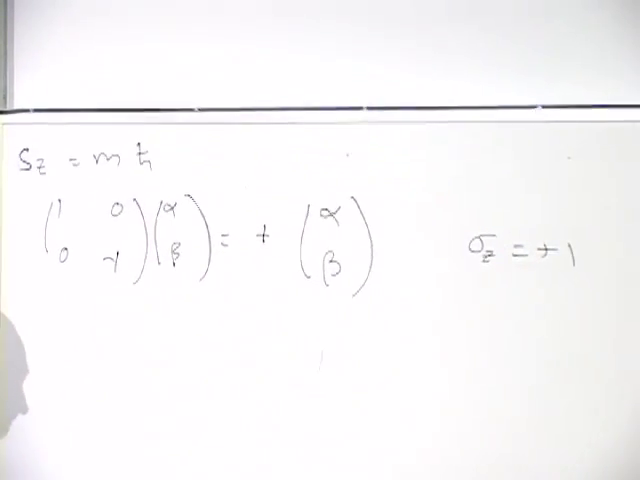
\includegraphics[width=0.74\textwidth]{lecture_08_figure_02.png}
\caption{Phương trình giá trị riêng \(+1\) của \(\sigma_z\) tác dụng lên một spinor hai thành phần.}
\lectureframe{00:34:57}
\end{figure}

Với trị riêng \(+1\), phép nhân theo từng hàng cho
\begin{equation}
\begin{pmatrix}
1\cdot\alpha+0\cdot\beta\\
0\cdot\alpha-\beta
\end{pmatrix}
=
\begin{pmatrix}
\alpha\\
-\beta
\end{pmatrix}
=
\begin{pmatrix}
\alpha\\
\beta
\end{pmatrix}.
\end{equation}
Phương trình trên tự động thỏa mãn, còn phương trình dưới cho \(-\beta=\beta\), do đó \(\beta=0\). Điều kiện chuẩn hóa đòi hỏi \(|\alpha|=1\); chọn pha tổng thể không quan trọng sao cho \(\alpha=1\),
\begin{equation}
|+z\rangle=
\begin{pmatrix}
1\\
0
\end{pmatrix}.
\end{equation}

Với trị riêng \(-1\),
\begin{equation}
\begin{pmatrix}
\alpha\\
-\beta
\end{pmatrix}
=
\begin{pmatrix}
-\alpha\\
-\beta
\end{pmatrix}.
\end{equation}
Bây giờ phương trình dưới tự động thỏa mãn, còn phương trình trên cho \(\alpha=-\alpha\), nên \(\alpha=0\). Chọn \(\beta=1\) ta được
\begin{equation}
|-z\rangle=
\begin{pmatrix}
0\\
1
\end{pmatrix}.
\end{equation}

Bây giờ hãy đổi thí nghiệm và đo \(S_x\). Vì
\begin{equation}
\sigma_x
\begin{pmatrix}
\alpha\\
\beta
\end{pmatrix}
=
\begin{pmatrix}
0\cdot\alpha+\beta\\
\alpha+0\cdot\beta
\end{pmatrix}
=
\begin{pmatrix}
\beta\\
\alpha
\end{pmatrix},
\end{equation}
phương trình \(+1\) trở thành
\begin{equation}
\begin{pmatrix}
\beta\\
\alpha
\end{pmatrix}
=
\begin{pmatrix}
\alpha\\
\beta
\end{pmatrix}.
\end{equation}
Hai phương trình theo thành phần, \(\beta=\alpha\) và \(\alpha=\beta\), là cùng một điều kiện. Chuẩn hóa cho
\begin{equation}
2|\alpha|^2=1,
\end{equation}
nên một lựa chọn thuận tiện là
\begin{equation}
|+x\rangle
=
\frac{1}{\sqrt2}
\begin{pmatrix}
1\\
1
\end{pmatrix}.
\end{equation}

\begin{figure}[t]
\centering
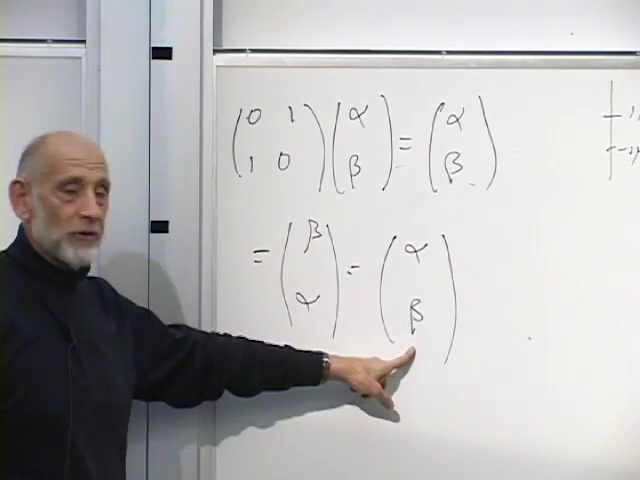
\includegraphics[width=0.74\textwidth]{lecture_08_figure_03.png}
\caption{Với trị riêng \(+1\), \(\sigma_x\) hoán đổi hai thành phần, nên cần \(\alpha=\beta\).}
\lectureframe{00:39:42}
\end{figure}

\begin{classroomqa}
\lecturetimestamp{00:40:13}
\audiencequestion{Nếu bao gồm hệ số một phần hai, thì trị riêng có phải là một phần hai không?}
\lecturerresponse{Có. Ma trận Pauli \(\sigma_x\) có các trị riêng \(\pm1\), còn \(S_x=\sigma_x/2\) có các trị riêng \(\pm\tfrac12\).}
\end{classroomqa}

Với trị riêng \(-1\),
\begin{equation}
\begin{pmatrix}
\beta\\
\alpha
\end{pmatrix}
=
-
\begin{pmatrix}
\alpha\\
\beta
\end{pmatrix},
\end{equation}
nên
\begin{equation}
\beta=-\alpha,
\qquad
\alpha=-\beta.
\end{equation}
Đây lại là cùng một phương trình. Sau khi chuẩn hóa,
\begin{equation}
|-x\rangle
=
\frac{1}{\sqrt2}
\begin{pmatrix}
1\\
-1
\end{pmatrix}.
\end{equation}
Vì vậy, một chồng chập với hệ số bằng nhau của spin lên theo \(z\) và spin xuống theo \(z\) được phân cực dọc theo trục \(x\) dương, còn trạng thái cùng dạng với một dấu trừ tương đối thì được phân cực dọc theo trục \(x\) âm.

Đối với hướng \(y\),
\begin{equation}
\sigma_y
\begin{pmatrix}
\alpha\\
\beta
\end{pmatrix}
=
\begin{pmatrix}
-i\beta\\
i\alpha
\end{pmatrix}.
\end{equation}
Hai vectơ riêng đã chuẩn hóa là
\begin{equation}
|+y\rangle
=
\frac{1}{\sqrt2}
\begin{pmatrix}
1\\
i
\end{pmatrix},
\qquad
|-y\rangle
=
\frac{1}{\sqrt2}
\begin{pmatrix}
1\\
-i
\end{pmatrix},
\end{equation}
trừ một pha tổng thể. Cả hai trạng thái đều cho xác suất \(1/2\) đối với spin lên theo \(z\) và \(1/2\) đối với spin xuống theo \(z\). Pha tương đối \(i\), vốn không lộ ra trong hai xác suất đó, phân biệt sự phân cực theo \(y\) với sự phân cực theo \(x\). Các tổ hợp tuyến tính cũng mô tả spin phân cực theo những hướng tùy ý; phép tính ấy được để lại sau.

\begin{classroomqa}
\lecturetimestamp{00:44:22}
\audiencequestion{Dấu của thành phần \(i\) có phải đã được gán cho sai trị riêng của \(\sigma_y\) không?}
\lecturerresponse{Quả thật dấu ấy có thể đã được gán cho sai trị riêng. Ở đây việc gán còn chưa chắc chắn; nó không được ấn định theo trí nhớ.}
\end{classroomqa}

Phép kiểm tra trực tiếp là
\begin{align}
\sigma_y\frac{1}{\sqrt2}
\begin{pmatrix}
1\\
i
\end{pmatrix}
&=
\frac{1}{\sqrt2}
\begin{pmatrix}
-i\,i\\
i
\end{pmatrix}
=
\frac{1}{\sqrt2}
\begin{pmatrix}
1\\
i
\end{pmatrix},\\
\sigma_y\frac{1}{\sqrt2}
\begin{pmatrix}
1\\
-i
\end{pmatrix}
&=
\frac{1}{\sqrt2}
\begin{pmatrix}
(-i)(-i)\\
i
\end{pmatrix}
=
-\frac{1}{\sqrt2}
\begin{pmatrix}
1\\
-i
\end{pmatrix}.
\end{align}
Vì vậy \(+i\) thuộc về trị riêng \(+1\), còn \(-i\) thuộc về trị riêng \(-1\).\footnote{Cách gán được nói miệng vẫn chưa ngã ngũ sau vài lần đảo ngược; các dấu trình bày ở đây được cố định bởi phép nhân ma trận đã hiển thị.} Mọi trạng thái spin 1/2, kể cả mọi trạng thái phân cực theo một hướng tùy ý, đều là tổ hợp tuyến tính của \(|+z\rangle\) và \(|-z\rangle\).

\section{Spin 1 và spinor phụ thuộc vị trí}

Đối với spin \(1\), các giá trị có thể có của \(S_z\) là \(+1,0,-1\). Vì thế không gian trạng thái là ba chiều. Spin \(1\) là spin nguyên và tương ứng với thống kê boson. Ta tìm ba ma trận \(3\times3\) thỏa mãn cùng các hệ thức giao hoán của mômen góc.

Một biểu diễn đối xứng giữa ba hướng tọa độ được cho dưới đây.\footnote{Dấu của \(S_y\) theo ma trận nhìn thấy gần \(00{:}48{:}50\), và cũng được cố định bởi \([S_x,S_y]=iS_z\). Đảo dấu đó sẽ đảo ngược giao hoán tử cần có.}
\begin{equation}
\begin{aligned}
S_x
&=
i
\begin{pmatrix}
0&0&0\\
0&0&1\\
0&-1&0
\end{pmatrix},
&
S_y
&=
i
\begin{pmatrix}
0&0&1\\
0&0&0\\
-1&0&0
\end{pmatrix},\\
S_z
&=
i
\begin{pmatrix}
0&1&0\\
-1&0&0\\
0&0&0
\end{pmatrix}.
\end{aligned}
\end{equation}
Mỗi ma trận là \(i\) nhân với một ma trận phản đối xứng thực. Mỗi ma trận chứa một \(1\), một \(-1\), và một hàng cùng một cột triệt tiêu gắn với chính tọa độ của nó: hàng-cột thứ nhất cho \(S_x\), thứ hai cho \(S_y\), và thứ ba cho \(S_z\). Điều này cho một mẹo ghi nhớ hữu ích. Trong biểu diễn này \(S_z\) không ở dạng đường chéo.

Đặt
\begin{equation}
v=
\begin{pmatrix}
\alpha\\
\beta\\
\gamma
\end{pmatrix}.
\end{equation}
Khi đó
\begin{equation}
S_zv
=
\begin{pmatrix}
i\beta\\
-i\alpha\\
0
\end{pmatrix}.
\end{equation}
Với trị riêng \(+1\),
\begin{equation}
i\beta=\alpha,
\qquad
-i\alpha=\beta,
\qquad
0=\gamma.
\end{equation}
Suy ra \(\beta=-i\alpha\) và \(\gamma=0\). Chuẩn hóa cho \(2|\alpha|^2=1\), nên
\begin{equation}
|m=+1\rangle
=
\frac{1}{\sqrt2}
\begin{pmatrix}
1\\
-i\\
0
\end{pmatrix}.
\end{equation}
Với trị riêng \(-1\),
\begin{equation}
i\beta=-\alpha,
\qquad
-i\alpha=-\beta,
\qquad
0=-\gamma,
\end{equation}
do đó \(\beta=i\alpha\), \(\gamma=0\), và
\begin{equation}
|m=-1\rangle
=
\frac{1}{\sqrt2}
\begin{pmatrix}
1\\
i\\
0
\end{pmatrix}.
\end{equation}
Cuối cùng, phương trình trị riêng bằng 0 cho \(\alpha=\beta=0\), để \(\gamma\) tùy ý. Nghiệm chuẩn hóa của nó là
\begin{equation}
|m=0\rangle
=
\begin{pmatrix}
0\\
0\\
1
\end{pmatrix}.
\end{equation}
Không còn trị riêng nào khác: ba vectơ riêng này bao hết không gian ba chiều. Các hệ số \(1/\sqrt2\) không phải chỉ để cho đẹp. Về sau chính các hệ số ấy sẽ đi vào các dự đoán thực nghiệm định lượng khi đại số được áp dụng cho isospin.

\begin{classroomqa}
\lecturetimestamp{00:54:10}
\audiencequestion{Nên đọc các phần tử phức của những vectơ riêng spin 1 này như thế nào?}
\lecturerresponse{Với \(m=+1\) các thành phần là \(1/\sqrt2,-i/\sqrt2,0\); với \(m=-1\) chúng là \(1/\sqrt2,i/\sqrt2,0\); và với \(m=0\) chúng là \(0,0,1\).}
\end{classroomqa}

Những bộ ba ma trận khác cũng thỏa mãn cùng đại số và tương đương về mặt vật lý. Biểu diễn đối xứng ở trên hữu ích vì ba hướng được đối xử như nhau, và nó sẽ còn được dùng lại.

\subsection{Khôi phục vị trí}

Bây giờ ta xét lại chuyển động của hạt. Spin giao hoán với vị trí và với xung lượng, nên có thể chỉ định một trong hai cùng với một thành phần spin. Vị trí và xung lượng không giao hoán, và các thành phần spin khác nhau cũng không giao hoán với nhau.

Một hạt spin 1/2 đang chuyển động được mô tả bởi một spinor phụ thuộc vị trí,
\begin{equation}
\psi(x)=
\begin{pmatrix}
\psi_\uparrow(x)\\
\psi_\downarrow(x)
\end{pmatrix}.
\end{equation}
Các đại lượng
\begin{equation}
\rho_{\uparrow_z}(x)=|\psi_\uparrow(x)|^2,
\qquad
\rho_{\downarrow_z}(x)=|\psi_\downarrow(x)|^2
\end{equation}
là các mật độ xác suất đồng thời của vị trí và spin. Tổng của chúng,
\begin{equation}
\rho(x)=\psi^\dagger(x)\psi(x)
=|\psi_\uparrow(x)|^2+|\psi_\downarrow(x)|^2,
\end{equation}
là mật độ vị trí. Nếu biết hạt đã được phát hiện tại \(x\), thì các xác suất có điều kiện là
\begin{equation}
P(\uparrow_z\mid x)
=
\frac{|\psi_\uparrow(x)|^2}{\psi^\dagger(x)\psi(x)},
\qquad
P(\downarrow_z\mid x)
=
\frac{|\psi_\downarrow(x)|^2}{\psi^\dagger(x)\psi(x)},
\end{equation}
miễn là \(\rho(x)\neq0\). Vì vậy một electron được biểu diễn bởi một hàm sóng không gian hai thành phần, trong đó các biên độ spin cục bộ được phép biến thiên từ nơi này sang nơi khác.

Đối với một hạt spin 1 đang chuyển động, viết
\begin{equation}
\phi(x)=
\begin{pmatrix}
\phi_1(x)\\
\phi_2(x)\\
\phi_3(x)
\end{pmatrix}.
\end{equation}
Tại mỗi điểm trong không gian, ba thành phần tạo thành một vectơ trong cùng không gian spin đã dùng ở trên. Các hạt spin 1 có spin nguyên và là boson.

\begin{classroomqa}
\lecturetimestamp{01:00:10}
\audiencequestion{Bản thân \(\phi_1(x)\) có phải là xác suất cho kết quả spin 1 \(m=+1\) không?}
\lecturerresponse{Không. Nó là một biên độ trong cơ sở ba thành phần đã chọn. Để thu được một kết quả spin xác định, hãy lập bra của vectơ riêng chuẩn hóa tương ứng, chiếu trường lên nó, rồi lấy bình phương môđun.}
\end{classroomqa}

\begin{figure}[t]
\centering
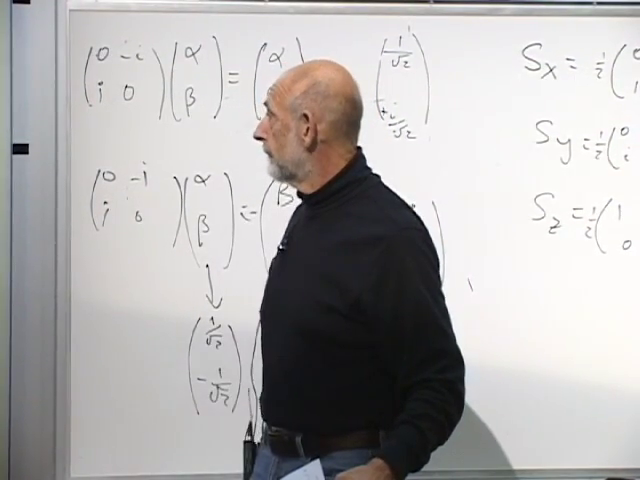
\includegraphics[width=0.82\textwidth]{lecture_08_figure_04.png}
\caption{Các vectơ riêng đã chuẩn hóa của \(\sigma_y\) cùng với ba ma trận spin 1/2.}
\lectureframe{01:00:12}
\end{figure}

Ví dụ,
\begin{equation}
\begin{aligned}
|m=+1\rangle
&=
\frac{1}{\sqrt2}
\begin{pmatrix}
1\\
-i\\
0
\end{pmatrix}
\\
\Longrightarrow\quad\langle m=+1|
&=
\frac{1}{\sqrt2}
\begin{pmatrix}
1&i&0
\end{pmatrix}.
\end{aligned}
\end{equation}
Vì thế biên độ chiếu là
\begin{align}
\langle m=+1|\phi(x)\rangle
&=
\frac{1}{\sqrt2}
\begin{pmatrix}
1&i&0
\end{pmatrix}
\begin{pmatrix}
\phi_1(x)\\
\phi_2(x)\\
\phi_3(x)
\end{pmatrix}\\
&=
\frac{\phi_1(x)+i\phi_2(x)}{\sqrt2}.
\end{align}
Áp dụng cùng quy tắc ấy cho cả ba vectơ riêng cho ta các mật độ phân giải theo spin.\footnote{Các công thức này hoàn tất đại số chiếu sau khi đã đính chính tường minh rằng \(\phi_1\) và \(\phi_2\) không nhất thiết phải là số thực. Nếu coi chúng là thực thì sẽ xóa nhầm sự giao thoa phân biệt các mật độ \(m=+1\) và \(m=-1\).}
\begin{align}
\rho_{+1}(x)
&=
\frac12\left|\phi_1(x)+i\phi_2(x)\right|^2,\\
\rho_{-1}(x)
&=
\frac12\left|\phi_1(x)-i\phi_2(x)\right|^2,\\
\rho_0(x)
&=
|\phi_3(x)|^2.
\end{align}
Chúng thỏa mãn
\begin{equation}
\begin{aligned}
\rho_{+1}(x)+\rho_{-1}(x)+\rho_0(x)
&=
|\phi_1(x)|^2+|\phi_2(x)|^2
\\
&\quad{}+|\phi_3(x)|^2
\\
&=
\phi^\dagger(x)\phi(x).
\end{aligned}
\end{equation}
Nếu điều kiện là hạt đã được phát hiện tại \(x\), thì
\begin{equation}
P(m\mid x)
=
\frac{\rho_m(x)}{\phi^\dagger(x)\phi(x)},
\end{equation}
miễn là \(\phi^\dagger(x)\phi(x)\neq0\). Quy tắc đo tổng quát luôn như nhau: lập bra của vectơ riêng chuẩn hóa mong muốn, chiếu trạng thái thực tế lên nó, rồi lấy bình phương môđun. Mật độ thu được vẫn giữ sự phụ thuộc vào vị trí.

Các ma trận spin cao hơn phức tạp hơn, nhưng nguyên lý không thay đổi.

\begin{classroomqa}
\lecturetimestamp{01:07:31}
\audiencequestion{Không gian trạng thái lớn đến mức nào đối với spin 3/2?}
\lecturerresponse{Nó có bốn trạng thái, với \(m=\tfrac32,\tfrac12,-\tfrac12,-\tfrac32\). Spin 2 có năm trạng thái.}
\end{classroomqa}

\begin{classroomqa}
\lecturetimestamp{01:07:55}
\audiencequestion{Vì sao phần trình bày có \(x,y,z\) mà không có hướng thời gian nào? Cách xử lý này có phải là phi tương đối tính không?}
\lecturerresponse{Cho đến đây thì là phi tương đối tính. Spin, cũng như khối lượng, được đặc trưng đơn giản nhất trong hệ quy chiếu nghỉ của hạt; mô tả của nó trong một hệ quy chiếu quán tính khác thu được bằng phép biến đổi Lorentz thích hợp. Bước tương đối tính đó được để lại sau.}
\end{classroomqa}

Phương trình Dirac cung cấp bối cảnh tương đối tính và giải thích vì sao hàm sóng bốn thành phần của nó chứa một bộ đôi spin.

\section{Các ma trận Dirac và spinor bốn thành phần}

Hàm sóng Dirac bốn thành phần thỏa mãn
\begin{equation}
i\frac{\partial\Psi}{\partial t}
=
-i\alpha_i\frac{\partial\Psi}{\partial x_i}
+m\beta\Psi,
\qquad i=1,2,3,
\end{equation}
trong đó một chỉ số không gian lặp lại thì được quy ước lấy tổng. Vì thế số hạng đạo hàm có nghĩa là
\begin{equation}
\alpha_1\frac{\partial\Psi}{\partial x}
+\alpha_2\frac{\partial\Psi}{\partial y}
+\alpha_3\frac{\partial\Psi}{\partial z}.
\end{equation}
Đối với một sóng phẳng, điều này trở thành phương trình đại số
\begin{equation}
\omega\Psi=(\alpha_i k_i+m\beta)\Psi.
\end{equation}

\begin{classroomqa}
\lecturetimestamp{01:11:32}
\audiencequestion{Hai lần xuất hiện của \(m\) có ký hiệu cùng một thứ không?}
\lecturerresponse{Không. Một cái đang được dùng làm chỉ số không gian, còn cái kia là khối lượng của hạt. Hãy đổi tên chỉ số không gian thành \(i\); khi \(i\) xuất hiện hai lần thì nó được lấy tổng từ \(1\) đến \(3\).}
\end{classroomqa}

Khi bình phương, toán tử tần số phải tái tạo hệ thức tương đối tính
\begin{equation}
\omega^2=\mathbf{k}^2+m^2.
\end{equation}
Do đó, các hạng bình phương đòi hỏi, với mỗi \(i\),
\begin{equation}
\alpha_i^2=I_4,
\qquad
\beta^2=I_4.
\end{equation}

\begin{classroomqa}
\lecturetimestamp{01:13:01}
\audiencequestion{\(\beta\) có khác nhau đối với từng thành phần trong bốn thành phần của \(\Psi\) không?}
\lecturerresponse{Không. Chỉ có một ma trận \(\beta\), tác dụng lên toàn bộ spinor bốn thành phần, và nó thỏa mãn \(\beta^2=I_4\).}
\end{classroomqa}

Các hạng chéo phải triệt tiêu. Đối với những hướng không gian khác nhau, và cả giữa mọi \(\alpha_i\) và \(\beta\), ta có
\begin{equation}
\alpha_i\alpha_j+\alpha_j\alpha_i=0
\quad (i\neq j),
\qquad
\alpha_i\beta+\beta\alpha_i=0.
\end{equation}
Tương đương,
\begin{equation}
\{\alpha_i,\alpha_j\}=2\delta_{ij}I_4,
\quad
\{\alpha_i,\beta\}=0,
\quad
\{\beta,\beta\}=2I_4.
\end{equation}
Mỗi ma trận phản giao hoán với mọi ma trận khác nó, còn phản giao hoán tử của nó với chính nó bằng hai lần ma trận đơn vị.

Nếu không có \(\beta\), thì ba ma trận Pauli đã cung cấp sẵn ba ma trận \(2\times2\) bình phương lên cho ma trận đơn vị và phản giao hoán từng đôi. Hạng khối lượng đòi hỏi một ma trận thứ tư như vậy. Không có ma trận \(2\times2\) thứ tư nào có các tính chất cần thiết, và các ma trận \(3\times3\) cũng không thỏa mãn đại số này. Vì vậy biểu diễn nhỏ nhất là \(4\times4\).

Một ma trận \(4\times4\) có thể được chia thành bốn khối \(2\times2\). Trong một biểu diễn thuận tiện,
\begin{equation}
\alpha_i=
\begin{pmatrix}
\sigma_i&0\\
0&-\sigma_i
\end{pmatrix},
\qquad i=1,2,3.
\end{equation}

\begin{figure}[t]
\centering
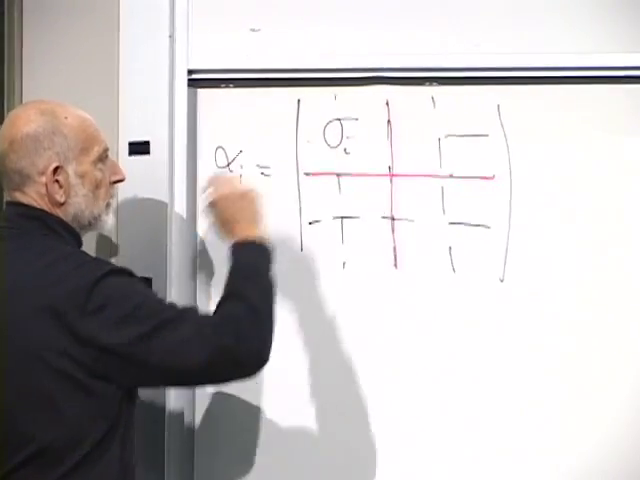
\includegraphics[width=0.68\textwidth]{lecture_08_figure_05.png}
\caption{Ma trận Dirac \(\alpha_i\) được viết thành các khối \(2\times2\), với \(\sigma_i\) và \(-\sigma_i\) trên đường chéo.}
\lectureframe{01:17:23}
\end{figure}

\begin{classroomqa}
\lecturetimestamp{01:17:41}
\audiencequestion{Trong biểu diễn trước đó, các khối \(\sigma_i\) có được sắp xếp theo cách ngược lại không?}
\lecturerresponse{Có. Trong một biểu diễn khác, chúng được đặt ngoài đường chéo. Hai cách sắp xếp là tương đương và liên hệ với nhau bằng một phép biến đổi đồng dạng.}
\end{classroomqa}

Trong biểu diễn hiện tại, ma trận còn lại là
\begin{equation}
\beta=
\begin{pmatrix}
0&I_2\\
I_2&0
\end{pmatrix},
\qquad
I_2=
\begin{pmatrix}
1&0\\
0&1
\end{pmatrix}.
\end{equation}
Phép nhân theo khối rút việc kiểm tra đại số \(4\times4\) về phép nhân thông thường của các ma trận \(2\times2\).

\begin{classroomqa}
\lecturetimestamp{01:19:17}
\audiencequestion{Biểu diễn trước đó có dùng một dấu khác hoặc một dạng chéo cho \(\beta\) không?}
\lecturerresponse{Nó dùng một cơ sở khác nhưng tương đương về mặt vật lý. Một phép đổi cơ sở trộn bốn thành phần của \(\Psi\) và làm thay đổi hình thức của các ma trận mà không làm thay đổi vật lý.}
\end{classroomqa}

Bốn phần tử của \(\Psi\) không phải là bốn tọa độ của không-thời gian. Chúng là các tọa độ trong không gian vectơ nhỏ nhất mà trên đó đại số phản giao hoán này có thể tác dụng. Có hai cấu trúc phân đôi phân biệt: sự chia thành các khối \(2\times2\) và cấu trúc Pauli hai thành phần bên trong mỗi khối. Đón trước cách diễn giải sẽ được thiết lập ở dưới, bốn khả năng có thể được sắp xếp thành
\begin{equation}
\begin{array}{c|cc}
& S_z=+\tfrac12 & S_z=-\tfrac12\\ \hline
\omega>0 & (\omega>0,+\tfrac12) & (\omega>0,-\tfrac12)\\
\omega<0 & (\omega<0,+\tfrac12) & (\omega<0,-\tfrac12)
\end{array}.
\end{equation}
Hàng dưới gồm các trạng thái electron tần số âm. Nó không phải là một hàng positron; positron sẽ được diễn giải như một lỗ trống trong tập đã lấp đầy của các trạng thái ấy.

\section{Sự nhân đôi năng lượng trong hệ nghỉ và positron}

Cấu trúc năng lượng hai nhánh bộc lộ rõ nhất tại xung lượng bằng 0. Khi \(\mathbf{k}=0\), trạng thái sóng phẳng là hằng theo không gian và số hạng đạo hàm theo không gian biến mất. Phương trình trong hệ nghỉ\footnote{Khung hình tại \(01{:}23{:}38\) vẫn còn tạm thời một hệ số \(i\) thừa ở hạng khối lượng; lời đính chính bằng lời tại \(01{:}24{:}05\) loại bỏ nó.} là
\begin{equation}
i\frac{\partial\Psi}{\partial t}=m\beta\Psi.
\end{equation}

\begin{figure}[t]
\centering
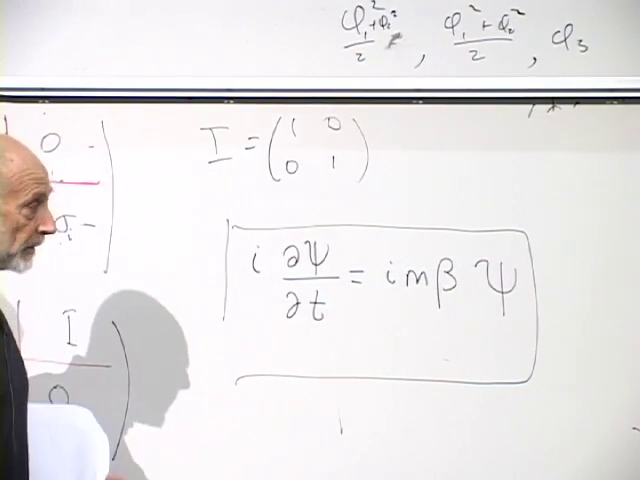
\includegraphics[width=0.76\textwidth]{lecture_08_figure_06.png}
\caption{Tại xung lượng bằng 0, các đạo hàm theo không gian triệt tiêu, để lại phương trình đã hiệu chỉnh trong hệ nghỉ \(i\partial_t\Psi=m\beta\Psi\).}
\lectureframe{01:23:38}
\end{figure}

Tách cột bốn thành phần thành một đối tượng hai thành phần ở trên và một đối tượng hai thành phần ở dưới:
\begin{equation}
\Psi=
\begin{pmatrix}
\psi_+\\
\psi_-
\end{pmatrix}.
\end{equation}

\begin{classroomqa}
\lecturetimestamp{01:24:47}
\audiencequestion{Các nhãn \(\psi_+\) và \(\psi_-\) đã có nghĩa là năng lượng dương và năng lượng âm chưa?}
\lecturerresponse{Chưa. Ở giai đoạn này, chúng chỉ là tên gọi cho các khối hai thành phần ở trên và ở dưới. Các tổ hợp năng lượng của chúng vẫn chưa được tìm ra.}
\end{classroomqa}

\begin{classroomqa}
\lecturetimestamp{01:25:10}
\audiencequestion{Vectơ cột bốn thành phần được chia đôi này biểu diễn cái gì?}
\lecturerresponse{Đó vẫn là cùng một spinor Dirac bốn thành phần, được sắp xếp cho khớp với dạng khối của các ma trận. Mỗi nửa là một đối tượng hai thành phần, và hai đối tượng như vậy hợp thành vectơ cột bốn thành phần ban đầu.}
\end{classroomqa}

Ma trận \(\beta\) hoán đổi hai khối:
\begin{equation}
\beta
\begin{pmatrix}
\psi_+\\
\psi_-
\end{pmatrix}
=
\begin{pmatrix}
\psi_-\\
\psi_+
\end{pmatrix}.
\end{equation}
Vì thế, phương trình trong hệ nghỉ trở thành
\begin{equation}
i\frac{\partial\psi_+}{\partial t}=m\psi_-,
\qquad
i\frac{\partial\psi_-}{\partial t}=m\psi_+.
\end{equation}

Có hai gợi ý tự nhiên. Lấy thêm một đạo hàm theo thời gian sẽ khử ghép hệ, nhưng lấy tổng và hiệu của hai phương trình thì chéo hóa chúng ngay lập tức. Thật vậy,
\begin{align}
i\frac{\partial}{\partial t}(\psi_++\psi_-)
&=m(\psi_++\psi_-),\\
i\frac{\partial}{\partial t}(\psi_+-\psi_-)
&=-m(\psi_+-\psi_-).
\end{align}
Đặt
\begin{equation}
\chi_+=\psi_++\psi_-,
\qquad
\chi_-=\psi_+-\psi_-,
\end{equation}
ta được hai phương trình độc lập,
\begin{equation}
i\partial_t\chi_+=m\chi_+,
\qquad
i\partial_t\chi_-=-m\chi_-.
\end{equation}
Với sự phụ thuộc theo tần số xác định \(e^{-i\omega t}\), tổng có
\begin{equation}
\omega=+m,
\end{equation}
trong khi hiệu có
\begin{equation}
\omega=-m.
\end{equation}
Đây chính là sự nhân đôi năng lượng dương và năng lượng âm đã thấy trong ví dụ một chiều trước đó: phương trình tương đối tính lại có các nghiệm electron năng lượng dương và năng lượng âm. Vì thế, sự nhân đôi theo khối tách thành các nhánh năng lượng dương và năng lượng âm. Các trạng thái thuần trong hệ nghỉ có thể được viết
\begin{equation}
\Psi_{\omega=+m}=
\begin{pmatrix}
\xi\\
\xi
\end{pmatrix},
\qquad
\Psi_{\omega=-m}=
\begin{pmatrix}
\xi\\
-\xi
\end{pmatrix},
\end{equation}
trong đó \(\xi\) vẫn là một đối tượng hai thành phần tùy ý.

Tổng và hiệu đã loại bỏ một cấu trúc bội hai, nhưng hai thành phần của \(\xi\) vẫn còn. Các ma trận Pauli tác dụng lên cặp còn lại này. Đây là cặp gắn với spin, như sẽ được kiểm tra bằng lập luận về phép quay và định luật bảo toàn ở dưới.

\begin{classroomqa}
\lecturetimestamp{01:32:23}
\audiencequestion{Có thể coi spin là cấu trúc bội hai ở ngoài và dấu năng lượng là cấu trúc bội hai ở trong không?}
\lecturerresponse{Có. Hai cách sắp thứ tự các thừa số là tương đương. Ta có thể hoán đổi chỉ số nào được viết trước; sự thay đổi ấy chỉ là sự xáo lại của bốn thành phần.}
\end{classroomqa}

Nhánh tần số âm dẫn tới cách diễn giải biển Dirac. Một tần số âm được gán cho năng lượng electron âm. Lấp đầy mọi trạng thái electron năng lượng âm sẽ hạ năng lượng xuống thấp nhất mà nguyên lý loại trừ cho phép, vì mỗi trạng thái fermion hoàn chỉnh chỉ có thể bị chiếm bởi một electron. Khi đó, biển năng lượng âm được lấp đầy hoàn toàn được gọi là chân không.

Nâng một electron từ biển đã lấp đầy này lên một trạng thái năng lượng dương. Kết quả chứa một electron năng lượng dương và một trạng thái năng lượng âm không bị chiếm. Lấy đi một năng lượng âm làm tăng năng lượng, nên lỗ trống có năng lượng kích thích dương; vì thiếu một electron nên nó cũng mang điện tích ngược dấu. Lỗ trống ấy là positron.

\begin{classroomqa}
\lecturetimestamp{01:32:57}
\audiencequestion{Có thể giải thích lại một lần nữa cách diễn giải về positron không?}
\lecturerresponse{Tổng của hai khối có tần số dương còn hiệu có tần số âm. Các nghiệm tần số âm là các trạng thái electron năng lượng âm, và chân không thu được bằng cách lấp đầy tất cả chúng. Nâng một electron đã bị chiếm lên năng lượng dương để lại đồng thời một electron năng lượng dương và một lỗ trống. Lỗ trống mang năng lượng dương và điện tích ngược dấu đó chính là positron.}
\end{classroomqa}

Vì vậy, phép đại số này đồng thời cho ra hai hệ quả: các nhánh năng lượng dương và âm, vốn trở thành cấu trúc hạt--phản hạt, và một cấu trúc hai thành phần còn lại gắn với spin một phần hai. Điểm nổi bật là cả hai đều xuất hiện từ những ma trận nhỏ nhất có thể thỏa mãn các quan hệ phản giao hoán tương đối tính. Vào thời điểm spin mới chỉ vừa xuất hiện như một tính chất thực nghiệm, cấu trúc toán học này lại tạo ra các hạt có spin đồng thời với một nhánh phản hạt; trong bối cảnh lịch sử ấy, kết quả đó là một điều gây chấn động.

\begin{classroomqa}
\lecturetimestamp{01:35:14}
\audiencequestion{Bản thân các electron năng lượng âm có phải là positron không?}
\lecturerresponse{Không. Các trạng thái electron năng lượng âm được lấp đầy trong chân không. Một positron là sự vắng mặt của một electron trong tập đã lấp đầy đó: một lỗ trống, không phải một electron năng lượng âm.}
\end{classroomqa}

Một lỗ trống có thể tham gia vào các chuyển dời. Một positron có năng lượng dương vì nó là sự vắng mặt của một electron năng lượng âm. Nếu một electron năng lượng dương lấp lỗ trống, electron và positron sẽ hủy nhau, nhưng năng lượng của chúng phải được mang đi, thông thường bởi các photon. Theo ngôn ngữ biển, một electron đã lấp vào một trạng thái năng lượng âm chưa bị chiếm. Cùng sự giải phóng năng lượng đó cũng có thể được hình dung như một electron kích thích trong nguyên tử rơi xuống mức thấp hơn: chuyển dời đi xuống phát ra các photon.

\begin{classroomqa}
\lecturetimestamp{01:36:39}
\audiencequestion{Tại sao các electron năng lượng âm ở mức cao hơn không rơi vào lỗ trống?}
\lecturerresponse{Câu hỏi đó trộn lẫn hai trường hợp. Một electron năng lượng dương lấp lỗ trống là sự hủy cặp electron--positron, trong đó các photon mang năng lượng đi. Một chuyển dời của một electron trong biển năng lượng âm là một quá trình khác, sẽ được xét ở dưới.}
\end{classroomqa}

Bản thân phép tính tại động lượng bằng không đã xác lập một suy biến bội hai sau khi dấu năng lượng được tách ra. Một suy biến của hai trạng thái, tự nó, không phải là bằng chứng rằng các trạng thái ấy mang mômen góc.

\begin{classroomqa}
\lecturetimestamp{01:37:44}
\audiencequestion{Làm thế nào phép tính tại động lượng bằng không chứng minh rằng cặp trạng thái còn lại là spin?}
\lecturerresponse{Cặp đó có thể được gọi là lên và xuống, và các ma trận Pauli xuất hiện trong phương trình đầy đủ, nhưng chỉ riêng điều đó vẫn chưa phải là chứng minh. Cần chỉ ra cặp ấy biến đổi thế nào dưới các phép quay trong không gian, hoặc việc gán cho nó spin làm cho tổng mômen góc được bảo toàn trong các tương tác và va chạm. Phần chứng minh ấy được hoãn lại.}
\end{classroomqa}

Đối với một trạng thái nghỉ năng lượng dương, khối trên và khối dưới bằng nhau,
\begin{equation}
\Psi_{\omega=+m}=
\begin{pmatrix}
\xi\\
\xi
\end{pmatrix}.
\end{equation}
Việc xác lập rằng \(\xi\) là một doublet mômen góc đòi hỏi lập luận về phép quay hoặc bảo toàn vừa mô tả; điều đó không suy ra chỉ từ việc đếm hai thành phần.

\begin{classroomqa}
\lecturetimestamp{01:40:46}
\audiencequestion{Một electron khác có thể hủy với positron ngay cả khi năng lượng của nó khác không?}
\lecturerresponse{Có. Các electron không giữ danh tính cá thể. Bất kỳ electron sẵn có nào cũng có thể lấp lỗ trống, và những khác biệt về năng lượng và động lượng ban đầu được phản ánh trong số lượng cũng như năng lượng của các photon phát ra.}
\end{classroomqa}

Bức tranh lỗ trống cũng giải thích một chuyển dời hoàn toàn bên trong biển năng lượng âm. Giả sử một trạng thái năng lượng âm đang bị chiếm chuyển vào lỗ trống. Lỗ trống ban đầu được lấp đầy, nhưng trạng thái mà electron ấy xuất phát từ đó nay lại trống. Lỗ trống đã di chuyển. Tương đương, positron đã đổi năng lượng của nó và đã phát ra bức xạ.

\begin{classroomqa}
\lecturetimestamp{01:42:12}
\audiencequestion{Tại sao các mức năng lượng âm lân cận không thể lần lượt rơi vào lỗ trống?}
\lecturerresponse{Chúng có thể làm cho lỗ trống chuyển từ mức này sang mức khác. Một electron rơi vào lỗ trống cũ để lại một lỗ trống mới tại năng lượng trước đó của nó, nên positron ban đầu trở thành một positron có năng lượng khác. Hiệu năng lượng được các photon mang đi.}
\end{classroomqa}

\begin{classroomqa}
\lecturetimestamp{01:44:39}
\audiencequestion{Tại sao điều này không tạo ra một chuỗi bức xạ đi xuống vô tận?}
\lecturerresponse{Vì năng lượng và động lượng phải được bảo toàn đồng thời. Hai định luật bảo toàn đó không cho phép quá trình không bị ràng buộc này. Cùng vấn đề ấy cũng nảy sinh đối với một electron tự do thông thường: nó không thể cứ đơn giản tiếp tục hạ năng lượng của mình bằng cách phát các photon trong không gian trống.}
\end{classroomqa}
\chapter{Lagrangian, các trường và các quá trình hạt cục bộ}

Các trường boson, các trường fermion và trường điện từ đều tuân theo những phương trình kiểu sóng. Các phương trình ấy chứa chính các trường cùng với các đạo hàm theo không gian và thời gian của chúng. Người ta có thể viết riêng một phương trình chuyển động cho từng trường, nhưng một Lagrangian gom toàn bộ hệ vào một biểu thức cô đọng duy nhất. Áp dụng quy tắc Euler--Lagrange cho biểu thức đó sẽ cho ra các phương trình của mọi trường cùng một lúc.

Cách xây dựng này liên hệ chặt chẽ với nguyên lý tác dụng dừng. Ở đây, nhiệm vụ trước mắt cụ thể hơn: xác định một Lagrangian trường phụ thuộc vào những gì, dùng nó để thu được một vài phương trình cổ điển, rồi sau đó diễn giải lại chính các biểu thức trường ấy theo cơ học lượng tử. Trong lý thuyết lượng tử, Lagrangian chi phối chuyển động và tương tác của hạt, và rốt cuộc là các biên độ cũng như tiết diện của va chạm.

\section{Mã gọn cho các phương trình trường}

Đối với một trường vô hướng, mật độ Lagrangian phụ thuộc vào trường và các đạo hàm bậc nhất của nó,
\begin{equation}
\mathcal L
=
\mathcal L\!\left(\phi,\partial_t\phi,\partial_x\phi,\ldots\right)
=
\mathcal L\!\left(\phi,\partial_\mu\phi\right).
\end{equation}
Danh sách tường minh các đạo hàm theo thời gian và theo không gian thường hữu ích hơn khi tính toán; ký hiệu \(\partial_\mu\phi\) viết gọn chính danh sách đó dưới dạng tương đối tính.

\begin{figure}[htbp]
\centering
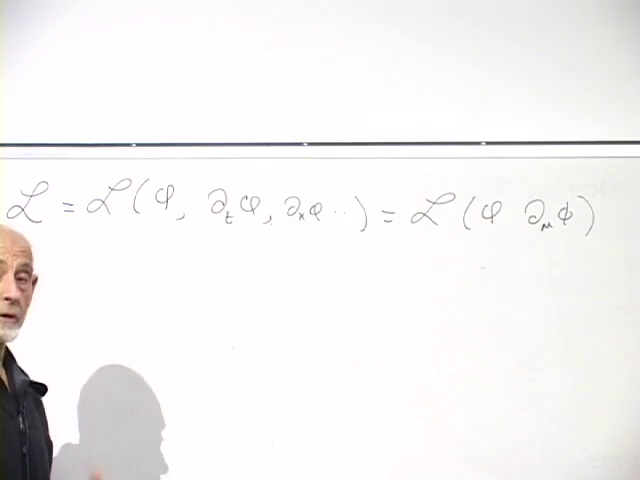
\includegraphics[width=0.82\textwidth]{lecture_09_figure_03.png}
\caption{Sự phụ thuộc của một Lagrangian trường vô hướng vào trường và các đạo hàm không-thời gian của nó.}
\lectureframe{00:03:56}
\end{figure}

Phương trình Euler--Lagrange cho trường là
\begin{equation}
\frac{\partial}{\partial t}
\frac{\partial\mathcal L}{\partial\dot\phi}
+
\frac{\partial}{\partial x}
\frac{\partial\mathcal L}{\partial\phi_x}
+
\frac{\partial}{\partial y}
\frac{\partial\mathcal L}{\partial\phi_y}
+
\frac{\partial}{\partial z}
\frac{\partial\mathcal L}{\partial\phi_z}
=
\frac{\partial\mathcal L}{\partial\phi},
\end{equation}
trong đó
\begin{equation}
\dot\phi=\frac{\partial\phi}{\partial t},
\qquad
\phi_x=\frac{\partial\phi}{\partial x},
\qquad
\phi_y=\frac{\partial\phi}{\partial y},
\qquad
\phi_z=\frac{\partial\phi}{\partial z}.
\end{equation}
Nếu \(\mathcal L\) chứa nhiều trường, thì quy tắc này được áp dụng một lần cho mỗi trường. Kết quả là hệ các phương trình chuyển động.

Ví dụ vô hướng đơn giản nhất là
\begin{equation}
\begin{split}
\mathcal L
&=
\frac12\dot\phi^2
-\frac12\phi_x^2
-\frac12\phi_y^2
-\frac12\phi_z^2
-V(\phi)
\\
&=
\frac12\dot\phi^2-\frac12(\boldsymbol\nabla\phi)^2-V(\phi).
\end{split}
\end{equation}
Các hạng đạo hàm không gian mang dấu ngược với hạng đạo hàm theo thời gian. Lấy đạo hàm từng hạng cho
\begin{align}
\frac{\partial\mathcal L}{\partial\dot\phi}&=\dot\phi,
&
\frac{\partial\mathcal L}{\partial\phi_i}&=-\phi_i,
&
\frac{\partial\mathcal L}{\partial\phi}&=-V'(\phi),
\end{align}
và do đó
\begin{equation}
\ddot\phi-\nabla^2\phi=-V'(\phi).
\end{equation}

\begin{figure}[htbp]
\centering
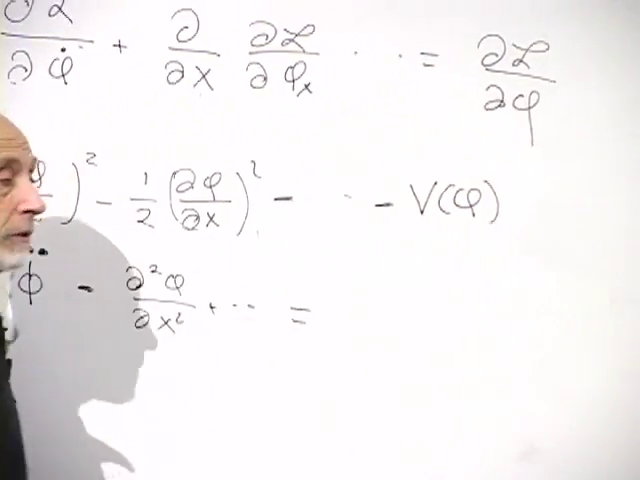
\includegraphics[width=0.74\textwidth]{lecture_09_figure_04.png}
\caption{Phương trình Euler--Lagrange, Lagrangian trường vô hướng và phương trình trường do \(V(\phi)\) sinh ra.}
\lectureframe{00:08:23}
\end{figure}

Đây là phương trình do Lagrangian vô hướng sinh ra.\editorialnote{Khung hình được giữ lại bị cắt ở mép trái; phần hoàn chỉnh được hiển thị được xác định từ phép suy dẫn bằng lời ngay xung quanh.}

Ở đây \(V(\phi)\) là mật độ thế năng của trường. Một đóng góp hằng vào \(V\) không ảnh hưởng gì đến phương trình này vì đạo hàm của nó triệt tiêu. Một thế tuyến tính là khả dĩ về mặt đại số, nhưng nó không có cận dưới: năng lượng của trường có thể chạy xuống âm vô cùng. Vì vậy, ví dụ ổn định đầu tiên là
\begin{equation}
V(\phi)=\frac12m^2\phi^2,
\qquad
V'(\phi)=m^2\phi,
\end{equation}
từ đó cho
\begin{equation}
\ddot\phi-\nabla^2\phi=-m^2\phi.
\end{equation}

Để làm rõ ý nghĩa của \(m\), hãy thế một sóng phẳng,
\begin{equation}
\phi(\mathbf x,t)=\phi_0e^{i\omega t-i\mathbf k\cdot\mathbf x}.
\end{equation}
Khi đó
\begin{equation}
\ddot\phi=-\omega^2\phi,
\qquad
\nabla^2\phi=-\mathbf k^2\phi,
\end{equation}
nên phương trình sóng trở thành
\begin{equation}
-\omega^2\phi+\mathbf k^2\phi=-m^2\phi.
\end{equation}
Sau khi khử \(\phi\),
\begin{equation}
\omega^2=\mathbf k^2+m^2.
\end{equation}
Trong hệ đơn vị \(\hbar=c=1\), tần số là năng lượng và số sóng là xung lượng. Do đó
\begin{equation}
E^2=\mathbf p^2+m^2,
\end{equation}
hoặc, khi khôi phục các lũy thừa của \(c\), \(E^2=\mathbf p^2c^2+m^2c^4\). Tham số \(m\) là khối lượng của một lượng tử của trường.

Tính bất biến tương đối tính có thể được áp đặt ngay ở mức biểu thức gọn. Nếu \(\mathcal L\) là một vô hướng Lorentz, thì các phương trình chuyển động của nó là bất biến Lorentz. Dấu tương đối giữa các đạo hàm theo thời gian và theo không gian chính là dấu không-thời gian quen thuộc của thuyết tương đối hẹp.

\section{Tính phi tuyến và các trường cổ điển ghép cặp}

Các lũy thừa cao hơn của trường đưa vào một kiểu hành vi mới. Nếu
\begin{equation}
V(\phi)=\frac12m^2\phi^2+g\phi^3,
\end{equation}
thì
\begin{equation}
\ddot\phi-\nabla^2\phi=-m^2\phi-3g\phi^2.
\end{equation}
Các hạng bậc hai trong Lagrangian cho những phương trình tuyến tính theo trường. Các hạng bậc ba và cao hơn cho những phương trình phi tuyến.

Sự phân biệt ấy thấy rõ trong chuyển động của các gói sóng. Với một phương trình tuyến tính, có thể cộng một gói truyền sang phải với một gói truyền sang trái để được một nghiệm khác. Chúng chồng lấp và giao thoa với nhau trong một lúc, rồi đi xuyên qua nhau và xuất hiện trở lại với hình dạng ban đầu. Khi có các hạng phi tuyến, các gói ảnh hưởng lẫn nhau. Chúng có thể tán xạ, biến dạng hoặc vỡ thành những sóng phức tạp hơn. Sự giao thoa tạm thời của sóng tuyến tính không phải là tương tác; một biến đổi kéo dài trong các gói là dấu hiệu của tính phi tuyến.

Mẫu hình ấy cũng xuất hiện với hai trường vô hướng. Hãy đặt
\begin{align}
\mathcal L
&=
\frac12(\partial_\mu\phi)(\partial^\mu\phi)
+\frac12(\partial_\mu\rho)(\partial^\mu\rho)
-V(\phi,\rho),
\\
V(\phi,\rho)
&=
\frac12m^2\phi^2+\frac12M^2\rho^2+\rho\phi^2.
\end{align}
Không có hạng cuối, hai phương trình là độc lập,
\begin{equation}
\ddot\phi-\nabla^2\phi=-m^2\phi,
\qquad
\ddot\rho-\nabla^2\rho=-M^2\rho.
\end{equation}
Chúng mô tả các lượng tử của hai loại, với khối lượng \(m\) và \(M\). Khi đưa thêm hạng trộn vào,
\begin{align}
\ddot\phi-\nabla^2\phi&=-m^2\phi-2\rho\phi,
\\
\ddot\rho-\nabla^2\rho&=-M^2\rho-\phi^2.
\end{align}
Mỗi phương trình giờ đây đều chứa trường kia. Các phương trình vừa ghép cặp vừa phi tuyến: một gói \(\phi\) tán xạ một gói \(\rho\), và ngược lại. Các hạng đạo hàm chi phối hệ thức năng lượng--xung lượng, các hạng bậc hai không đạo hàm xác định khối lượng, còn hạng trộn bậc cao hơn mã hóa tương tác. Đây là khuôn mẫu cổ điển cơ bản.

\section{Trường Dirac và một ghép vô hướng}

Đối với một trường Dirac, phương trình là bậc nhất theo thời gian. Dưới dạng viết tắt một chiều, với việc mở rộng sang ba phương không gian đã được ngầm hiểu, cấu trúc các hạng của nó là
\begin{equation}
i\dot\Psi
\simeq
i\alpha\frac{\partial\Psi}{\partial x}+m\beta\Psi,
\qquad
i\boldsymbol\alpha\cdot\boldsymbol\nabla\Psi
=i\sum_i\alpha_i\frac{\partial\Psi}{\partial x_i}.
\end{equation}
Các ma trận \(\alpha_i\) và \(\beta\) tác dụng lên các thành phần của \(\Psi\). Một Lagrangian tương ứng chứa một hạng tuyến tính theo \(\partial_t\Psi\), một song tuyến tính đạo hàm không gian có chứa \(\alpha_i\), và song tuyến tính khối lượng \(m\Psi^\dagger\beta\Psi\). Ở đây chỉ cần sự kiện về cấu trúc đó.\editorialnote{Dấu, ngoặc và vị trí đặt của \(i\) trong Lagrangian Dirac được thử viết ra được nguồn để ngỏ một cách tường minh. Từ đó không suy ra công thức chính xác nào phụ thuộc quy ước.}

\begin{figure}[htbp]
\centering
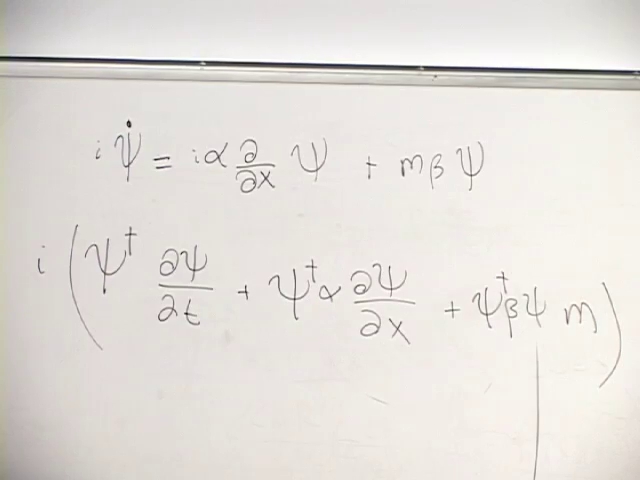
\includegraphics[width=0.76\textwidth]{lecture_09_figure_05.png}
\caption{Các hạng đạo hàm theo thời gian, đạo hàm theo không gian và khối lượng trong phần thảo luận về trường Dirac.}
\lectureframe{00:25:37}
\end{figure}

\begin{classroomqa}
\lecturetimestamp{00:26:37}
\audiencequestion{Dấu ngoặc trong Lagrangian Dirac thử viết ra có được đặt đúng không, với \(i\) nhân toàn bộ biểu thức?}
\lecturerresponse{Vị trí đặt ấy không được chốt ở đây một cách chắc chắn, và điều đó không cần cho ý chính về mặt cấu trúc: tồn tại một Lagrangian sinh ra phương trình Dirac.}
\end{classroomqa}

Bây giờ thêm một trường vô hướng \(\phi\). Tích ngây thơ \(\Psi^\dagger\Psi\,\phi\) không phải là một vô hướng Lorentz. Chèn cùng ma trận Dirac xuất hiện trong hạng khối lượng vào, ta được
\begin{equation}
\mathcal L_{\mathrm{int}}
\propto
\Psi^\dagger\beta\Psi\,\phi.
\end{equation}
Tương đương, \(\Psi^\dagger\beta\Psi\) là song tuyến tính Dirac vô hướng. Lấy biến phân của Lagrangian đầy đủ sẽ thêm một hạng tỉ lệ với \(\phi\) vào phương trình Dirac và một nguồn tỉ lệ với \(\Psi^\dagger\beta\Psi\) vào phương trình vô hướng. Hai trường tán xạ lẫn nhau.

\begin{classroomqa}
\lecturetimestamp{00:28:03}
\audiencequestion{Ma trận \(\beta\) được chèn vào tương tác vô hướng--fermion có phải chính là \(\beta\) xuất hiện trong hạng khối lượng Dirac không?}
\lecturerresponse{Đúng. Đó là cùng một ma trận Dirac.}
\end{classroomqa}

Phép so sánh
\begin{equation}
m\Psi^\dagger\beta\Psi
\qquad\hbox{and}\qquad
\Psi^\dagger\beta\Psi\,\phi
\end{equation}
khiến ghép đó trông như một tham số khối lượng được thay bằng một trường vô hướng. Nhận xét này sẽ quay lại khi ta xét một trường có giá trị chân không khác không ở gần cuối.

Cho đến đây, cách diễn giải vẫn là cổ điển: các gói sóng tán xạ những gói sóng khác. Cùng phép đại số ấy có một ý nghĩa hạt sắc nét hơn khi các trường trở thành toán tử.

\section{Các lũy thừa của trường lượng tử làm gì}

Một trường lượng tử vô hướng thực chứa cả toán tử tạo lẫn toán tử hủy. Về sơ đồ,
\begin{equation}
\phi(x)\sim A^+(x)+A^-(x),
\end{equation}
trong đó \(A^+\) tạo ra một lượng tử còn \(A^-\) hủy một lượng tử. Do đó, \(\phi^3(x)\) chứa bốn kiểu quá trình cục bộ:
\begin{equation}
\phi^3
\sim
(A^+)^3+(A^+)^2A^-+A^+(A^-)^2+(A^-)^3,
\end{equation}
trong đó các chi tiết về thứ tự và các hệ số số học được lược bỏ trong cách đọc sơ đồ này. Bốn sự thay đổi số hạt là
\begin{equation}
3\longrightarrow0,
\qquad
0\longrightarrow3,
\qquad
2\longrightarrow1,
\qquad
1\longrightarrow2.
\end{equation}
Ba thừa số trường đều tác dụng tại cùng một điểm \(x\). Vì thế một hạng bậc ba đơn lẻ bao gồm sự hủy ba hạt, sự tạo ba hạt, sự hợp nhất của hai lượng tử thành một, và sự phân rã của một lượng tử thành hai. Trong một biên độ vật lý, về sau một số cách đọc cục bộ này có thể bị loại bởi bảo toàn năng lượng--xung lượng, nhưng tất cả chúng đều có mặt ngay trong chính tích toán tử.

Các hạng tự do bậc hai có vai trò khác. Trước hết hãy tạm bỏ qua hệ số chuẩn hóa của hiệu giữa hai điểm lân cận \(x\) và \(x'\):
\begin{equation}
\partial_x\phi
\ \propto\
\phi(x)-\phi(x').
\end{equation}
Bình phương rồi khai triển cho cấu trúc hạng
\begin{align}
\frac12(\partial_x\phi)^2
&\ \propto\
\frac12\bigl[\phi(x)-\phi(x')\bigr]^2
\\
&=
\frac12\phi(x)^2
+\frac12\phi(x')^2
-\phi(x)\phi(x').
\end{align}
Mỗi bình phương tại cùng một điểm có vài cách đọc theo toán tử: nó có thể tạo hai lượng tử, hủy hai lượng tử, hoặc hủy rồi tái tạo một lượng tử ngay tại điểm đó. Các hạng ấy không vận chuyển một hạt. Hạng chéo có thể hủy một lượng tử tại \(x'\) và tạo nó tại \(x\), hoặc ngược lại. Vì vậy nó hoạt động như một hạng nhảy giữa các láng giềng gần nhất. Các thừa số lặp lại mang một hạt từ \(x\) sang \(x'\), rồi sang \(x''\), và tiếp tục như thế. Các hạng đạo hàm bậc hai chi phối sự lan truyền tự do; các hạng bậc ba và cao hơn thì tán xạ, tạo và hủy hạt.

\begin{classroomqa}
\lecturetimestamp{00:36:07}
\audiencequestion{Biểu diễn sai phân hữu hạn của đạo hàm có nên bao gồm độ tách \(x-x'\) không?}
\lecturerresponse{Có. Nếu gọi độ tách đó là \(L\) thì sau khi bình phương hiệu, ta có thêm thừa số \(L^{-2}\). Thừa số số học ấy làm thay đổi hệ số nhưng không làm đổi cách diễn giải theo bước nhảy.}
\end{classroomqa}

Khôi phục độ tách vào thì được
\begin{align}
\frac12(\partial_x\phi)^2
&\longrightarrow
\frac{1}{2L^2}\bigl[\phi(x)-\phi(x')\bigr]^2
\\
&=
\frac{1}{2L^2}\phi(x)^2
+\frac{1}{2L^2}\phi(x')^2
-\frac{1}{L^2}\phi(x)\phi(x').
\end{align}

Hạng khối lượng cũng là bậc hai nhưng không chứa đạo hàm:
\begin{equation}
\frac12m^2\phi(x)^2.
\end{equation}
Cách đọc một-hạt của nó là một lượng tử tới bị hấp thụ và phát lại tại cùng một điểm. Nó không làm lượng tử chuyển chỗ; nó gán trọng số, hay theo nghĩa đó là đếm, sự hiện diện của nó ở đó. Cùng bình phương toán tử ấy cũng chứa các cách đọc tạo hai hạt và hủy hai hạt của nó. Vì vậy, sự khác biệt có liên quan đến chuyển động là giữa một hạng chéo nối các điểm lân cận và một chèn khối lượng tác dụng trong một điểm.

\section{Đỉnh cục bộ của điện động lực học lượng tử}

Những phác họa sơ cấp về quá trình hạt này là khởi đầu của các biểu đồ Feynman. Ví dụ trung tâm là điện động lực học lượng tử, lý thuyết của electron, positron và photon.

Phương trình Dirac có các mode năng lượng dương và năng lượng âm. Theo ngôn ngữ cũ, \(\Psi\) chứa các toán tử hủy cho cả hai loại mode, còn \(\Psi^\dagger\) chứa các toán tử tạo tương ứng. Việc lấy đi một electron năng lượng âm được diễn giải lại thành việc tạo ra một positron năng lượng dương. Sau phép đổi nhãn đó, phân tích sơ đồ hữu ích là
\begin{align}
\Psi
&\sim
C^-_{e^-}+C^+_{e^+},
\\
\Psi^\dagger
&\sim
C^+_{e^-}+C^-_{e^+}.
\end{align}
Vì vậy \(\Psi\) hủy một electron hoặc tạo một positron, còn \(\Psi^\dagger\) tạo một electron hoặc hủy một positron. Trong lối viết tắt này không hàm ý chuẩn hóa, nhãn spin hay tích phân theo xung lượng nào.

Tương tác QED ghép dòng Dirac với thế vectơ điện từ. Trong ký hiệu theo thành phần được dùng ở đây, cấu trúc của nó là
\begin{equation}
\mathcal L_{\mathrm{QED,int}}
\sim
e\left(
\Psi^\dagger\Psi\,A_0
+
\Psi^\dagger\boldsymbol{\alpha}\Psi\mathbin{\boldsymbol{\cdot}}\mathbf A
\right),
\end{equation}
trong đó
\begin{equation}
J^0=\Psi^\dagger\Psi,
\qquad
\mathbf J=\Psi^\dagger\boldsymbol{\alpha}\Psi.
\end{equation}
Ký hiệu \(\sim\) là quan trọng: dấu tương đối giữa hạng thời gian và hạng không gian phụ thuộc vào quy ước metric và quy ước thế vectơ. Phát biểu bất biến là dòng bốn được co với thế bốn.\editorialnote{Nguồn cố định các thành phần thời gian và không gian của dòng nhưng không chốt một quy ước metric cho phép co theo thành phần.}

Trường photon \(A_\mu\) tự thân cũng chứa các toán tử tạo và hủy photon. Tính vectơ của nó còn mang theo phân cực của photon---một ``lá cờ'' chỉ hướng nhỏ bên cạnh xung lượng của nó.

\begin{classroomqa}
\lecturetimestamp{00:44:28}
\audiencequestion{Làm sao tương tác lại có thể là vô hướng khi \(A_\mu\) là một vectơ còn thoạt đầu thừa số fermion dường như là một vô hướng?}
\lecturerresponse{Các fermion cũng cung cấp một vectơ bốn: \(\Psi^\dagger\Psi\) là thành phần thời gian của nó còn \(\Psi^\dagger\boldsymbol\alpha\Psi\) là thành phần không gian. Co dòng đó với \(A_\mu\) sẽ cho một vô hướng.}
\end{classroomqa}

Nhân các nội dung toán tử của \(\Psi^\dagger\), \(\Psi\) và \(A_\mu\) cho ta bốn cách đọc quen thuộc của một đỉnh cục bộ:
\begin{enumerate}
\item một electron phát ra một photon;
\item một electron hấp thụ một photon;
\item một electron và một positron hủy nhau thành một photon;
\item một photon tạo ra một cặp electron--positron.
\end{enumerate}
Đối với cách đọc thứ nhất, \(\Psi\) hủy electron đi vào, \(\Psi^\dagger\) tạo electron đi ra, và trường photon tạo ra photon. Chọn phần hủy photon thì được sự hấp thụ. Chọn các phần của positron thì được hủy cặp hoặc tạo cặp. Một hạng cục bộ chứa toàn bộ họ quá trình đó.

Trong một sơ đồ dòng fermion, mũi tên trên một đường positron chỉ ngược với hướng truyền của positron. Với quy ước đó, mũi tên fermion đi liên tục qua mọi đỉnh QED được phép. Bốn cách đọc khác nhau ở chỗ chuyển các chân ngoài giữa phía đi vào và phía đi ra, chứ không phải ở chỗ bẻ gãy đường dòng fermion.

Mỗi cách đọc này đều mang cùng một hệ số \(e\), tức điện tích trong quy ước vi mô đang được dùng. Hệ số này là điện tích \(e\), không phải hằng số cấu trúc tinh tế, mặc dù hai đại lượng liên hệ chặt chẽ. Biên độ của đỉnh tỉ lệ với \(e\); sau khi kể hết các thừa số động học và chuẩn hóa, thang xác suất tương ứng tỉ lệ với \(e^2\).

\begin{classroomqa}
\lecturetimestamp{00:49:44}
\audiencequestion{Cách đọc từ photon sang electron--positron có cùng hệ số như các cách đọc khác của đỉnh không?}
\lecturerresponse{Có. Nó mang cùng hệ số điện tích \(e\).}
\end{classroomqa}

\begin{classroomqa}
\lecturetimestamp{00:49:59}
\audiencequestion{Có nhất thiết phải có một hệ số tỉ lệ, vì xác suất không có đơn vị không?}
\lecturerresponse{Trong quy ước vi mô tự nhiên đang được dùng, điện tích \(e\) là vô thứ nguyên. Nó đặt thang biên độ, còn bình phương của nó cung cấp thang xác suất.}
\end{classroomqa}

Một hình dung cụ thể là một electron đập vào một bức tường rồi dừng lại đột ngột. Có một xác suất nào đó để năng lượng và động lượng rời đi dưới dạng một photon. Thừa số điện từ sơ cấp trong biên độ bức xạ đó là \(e\), nên thang xác suất của nó chứa \(e^2\). Phát biểu này tách riêng thừa số ghép; xác suất thực tế còn phụ thuộc vào trạng thái của electron và vào động học.

\begin{figure}[htbp]
\centering
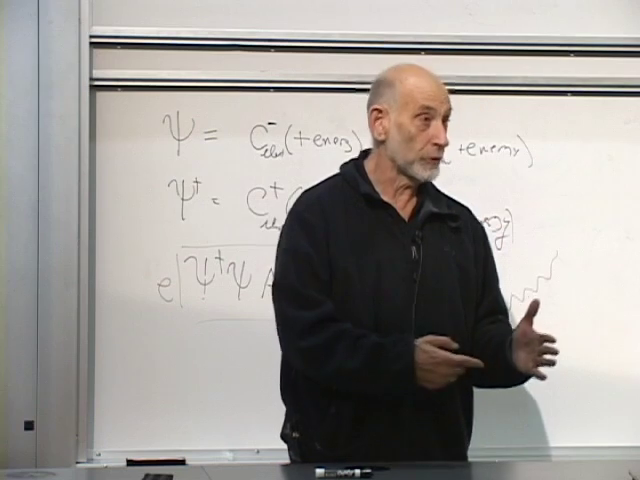
\includegraphics[width=0.78\textwidth]{lecture_09_figure_06.png}
\caption{Thành phần toán tử electron và positron của \(\Psi\) và \(\Psi^\dagger\), kèm một phác họa tương tác electron--photon.}
\lectureframe{00:50:39}
\end{figure}

\begin{classroomqa}
\lecturetimestamp{00:51:15}
\audiencequestion{Điện tích có đơn vị không?}
\lecturerresponse{Không, trong quy ước vi mô tự nhiên được dùng ở đây thì không. Điện tích vĩ mô thường được báo bằng coulomb, nhưng lý thuyết hạt đo điện tích tương đối với một đơn vị cơ bản được chọn. Trong đơn vị Planck hoặc các đơn vị tự nhiên khác, các đại lượng được biểu diễn bằng những số thuần túy.}
\end{classroomqa}

Sự tương phản này là về quy ước và thang đo. Coulomb thuận tiện cho dòng điện trong dây dẫn; một hằng ghép vô thứ nguyên thuận tiện cho các biên độ vi mô.\editorialnote{Một câu hỏi ngắn từ 00:52:37--00:53:15 về việc ``gom nhóm'' các hạng mang điện tích đã bị hỏng đáng kể và không thể phục dựng một cách xác định.}

Cả ba trường trong tương tác QED sơ cấp đều được lấy tại cùng một điểm không-thời gian. Bản thân đỉnh không được gán một độ trễ thời gian nội tại nào.

\begin{classroomqa}
\lecturetimestamp{00:53:19}
\audiencequestion{Sự hấp thụ rồi phát xạ lại electron cùng với sự phát xạ photon có đồng thời không, hay phương trình đã hàm sẵn một độ trễ?}
\lecturerresponse{Tại đỉnh sơ cấp, tất cả các toán tử đều được lấy tại cùng một điểm không-thời gian. Vì vậy quá trình cơ bản không chứa độ trễ nào giữa các tác động ấy.}
\end{classroomqa}

\begin{classroomqa}
\lecturetimestamp{00:53:57}
\audiencequestion{Mỗi đại lượng bảo toàn có phải được bảo toàn riêng rẽ không?}
\lecturerresponse{Có. Điện tích là một trong các đại lượng phải được bảo toàn riêng rẽ.}
\end{classroomqa}

Bảo toàn điện tích thấy được cả trong sơ đồ lẫn trong đại số. Một quá trình biến một electron đi vào thành một positron đi ra sẽ đảo ngược điện tích và không phải là một đỉnh QED được phép. Khi vẽ thời gian hướng lên trên, mũi tên của electron đi theo thời gian lên trên còn mũi tên của positron chỉ xuống dưới; một đỉnh hợp lệ luôn có một mũi tên fermion đi xuyên qua. Về mặt đại số, tương tác chứa một \(\Psi\) và một \(\Psi^\dagger\). Toán tử thứ nhất làm tăng điện tích thêm một đơn vị khi nó hủy một electron hoặc tạo một positron, còn toán tử thứ hai làm giảm điện tích đi một đơn vị. Các tác dụng của chúng triệt tiêu nhau.

\begin{classroomqa}
\lecturetimestamp{00:56:05}
\audiencequestion{Biểu thức electron--photon được đóng khung có phải là toàn bộ Lagrangian QED không?}
\lecturerresponse{Không. Đó là hạng tương tác. Các hạng photon tự do bậc hai và các hạng Dirac bậc hai, vốn chi phối sự truyền, chưa được viết ra.}
\end{classroomqa}

\begin{classroomqa}
\lecturetimestamp{00:56:35}
\audiencequestion{Lagrangian cổ điển được suy ra, còn Lagrangian lượng tử thì được phỏng đoán và kiểm nghiệm, và cấu trúc động năng trừ thế năng có còn giữ trong cơ học lượng tử không?}
\lecturerresponse{Mô thức động năng trừ thế năng vẫn còn: các đạo hàm theo thời gian cung cấp dạng động năng, các gradient không gian khái quát hóa nó, còn các hạng trường không lấy đạo hàm cung cấp dạng thế năng. Lagrangian lượng tử là mô tả cơ bản hơn. Trong một trạng thái chứa rất nhiều lượng tử, chính Lagrangian đó sinh ra các phương trình sóng cổ điển. Các Lagrangian ứng viên được đề xuất bằng các nguyên lý vật lý và lý thuyết sâu hơn, rồi được xác lập hoặc bác bỏ thông qua các thí nghiệm va chạm.}
\end{classroomqa}

Giới hạn số chiếm lớn giải thích vì sao cùng một biểu thức có thể chi phối một lý thuyết hạt lượng tử và các sóng cổ điển của nó. Sự phù hợp này không phải là một phép màu riêng rẽ được áp đặt về sau; trường cổ điển là hành vi tập thể của nhiều lượng tử. Ngược lại, các va chạm thực nghiệm bộc lộ các đỉnh sơ khai đủ trực tiếp để xác định các tương tác của QED và Mô hình Chuẩn với độ chính xác rất cao.

\section{Crossing và các định luật bảo toàn không-thời gian}

Các chân của một đỉnh cục bộ có thể được chuyển chéo giữa vị trí đi vào và đi ra. Một hạt đi ra khi được chuyển sang phía đi vào sẽ được diễn giải lại thành phản hạt của nó, và ngược lại. Theo nghĩa này, cùng một toán tử electron--positron--photon có các cách đọc cục bộ tương ứng với phát xạ, hấp thụ, hủy cặp, tạo cặp, và thậm chí cả trường hợp mọi hạt đều đi vào.

\begin{classroomqa}
\lecturetimestamp{00:59:34}
\audiencequestion{Nếu quay một sơ đồ đỉnh cơ bản, nó có còn là một cách đọc cục bộ hợp lệ không?}
\lecturerresponse{Có. Các chân ngoài của nó có thể được chuyển giữa vị trí đi vào và đi ra, kèm theo sự diễn giải lại tương ứng hạt--phản hạt.}
\end{classroomqa}

Cách đọc từ toán tử địa phương này vẫn chưa phải là một quá trình vật lý hoàn chỉnh. Biên độ của nó phải được lấy tích phân trên mọi điểm không-thời gian mà tại đó đỉnh tương tác có thể xảy ra. Tích phân theo thời gian áp đặt bảo toàn năng lượng, còn tích phân theo không gian áp đặt bảo toàn động lượng. Một hình dung trong đó một electron, một positron và một photon đều biến mất vào chân không xuất hiện như một cách đọc cục bộ hình thức, nhưng biên độ đã lấy tích phân triệt tiêu vì quá trình đó không thể bảo toàn năng lượng và động lượng.

\begin{classroomqa}
\lecturetimestamp{01:00:30}
\audiencequestion{Hình ảnh mọi hạt đều đi vào có nghĩa là một electron, một positron và một photon có thể biến mất vào hư không sao?}
\lecturerresponse{Đó là một cách đọc của toán tử cục bộ, nhưng biên độ vật lý còn bao gồm tích phân theo vị trí của đỉnh. Các tích phân ấy áp đặt bảo toàn năng lượng và động lượng, nên quá trình bị cấm về mặt động học này có biên độ bằng 0.}
\end{classroomqa}

\begin{classroomqa}
\lecturetimestamp{01:01:57}
\audiencequestion{Cách đọc ngược lại từ chân không sang electron--positron--photon có tồn tại không, và các quá trình bị loại có biến mất sau khi lấy tích phân không?}
\lecturerresponse{Cách đọc cục bộ ngược lại cũng có mặt. Lấy tích phân theo không gian và thời gian loại bỏ mọi quá trình không tương thích với các định luật bảo toàn.}
\end{classroomqa}

Các đạo hàm trong Lagrangian phù hợp với khai triển toán tử mà không cần lấy đạo hàm chính các ký hiệu tạo và hủy. Một trường có dạng sơ đồ
\begin{equation}
\Psi(x)
\sim
\int d^3k\,
\bigl[
C(\mathbf k)e^{i\mathbf k\cdot\mathbf x-i\omega t}
+\cdots
\bigr].
\end{equation}
Các toán tử \(C(\mathbf k)\) là các hệ số trong khai triển không-thời gian này. Đạo hàm tác dụng lên các sóng phẳng, làm xuất hiện \(\mathbf k\) hoặc \(\omega\).

\begin{classroomqa}
\lecturetimestamp{01:02:27}
\audiencequestion{Khi lấy đạo hàm một khai triển trường, có lấy đạo hàm chính toán tử tạo không?}
\lecturerresponse{Không. Trong khai triển này, các toán tử tạo và hủy độc lập với tọa độ không-thời gian. Các đạo hàm tác dụng lên các thừa số mũ và làm xuất hiện động lượng cùng tần số.}
\end{classroomqa}

\section{Nucleon và pion như một lý thuyết hiệu dụng}

Cùng ngôn ngữ này có thể mô tả proton, neutron và pion. Proton và neutron là các fermion được biểu diễn bởi các trường \(\Psi_p\) và \(\Psi_n\). Trong thảo luận đếm tương tác này, các trường pion được xem như các trường vô hướng với ba dạng điện tích,
\begin{equation}
\pi^+,
\qquad
\pi^-,
\qquad
\pi^0.
\end{equation}
Proton và \(\pi^+\) mang một đơn vị điện tích dương, \(\pi^-\) mang một đơn vị điện tích âm, còn neutron và \(\pi^0\) là trung hòa. Ở mức sâu hơn, pion là các hệ quark--phản quark, nhưng ban đầu có thể để ngỏ mô tả nội tại ấy.

Một danh sách sơ đồ các tích trường nucleon--pion bảo toàn điện tích là
\begin{equation}
\mathcal L_{N\pi}
\sim
\left\{
\Psi_p^\dagger\Psi_n\,\pi^+,\;
\Psi_n^\dagger\Psi_p\,\pi^-,\;
\Psi_p^\dagger\Psi_p\,\pi^0,\;
\Psi_n^\dagger\Psi_n\,\pi^0
\right\}.
\end{equation}
Ở đây chỉ hiển thị nội dung trường và các gán điện tích; các hệ số tương đối, dấu và cấu trúc ma trận-spinor chưa được cố định. Điện tích trên trường pion thứ nhất được cố định bằng cách xét một cách đọc cụ thể: một neutron cùng với một pion dương có thể tạo ra một proton, trong khi dùng một pion âm ở đó sẽ biến điện tích âm đi vào thành điện tích dương đi ra. Hạng liên hợp cho quá trình mang điện tích ngược lại.\editorialnote{Dấu của pion đã được sửa nhiều lần trong nguồn trước khi đi tới cặp bảo toàn điện tích được nêu ở đây; thứ tự hiển thị ghi lại cấu trúc sơ đồ cuối cùng đó.}

Mỗi hạng lại có vài cách đọc chéo. Chuyển một neutron đi ra sang phía đi vào sẽ biến nó thành một phản neutron đi vào. Vì thế đỉnh mang điện có thể mô tả một proton và một phản neutron kết hợp thành một \(\pi^+\), cũng như các quá trình như \(p\to n+\pi^+\) khi động học cho phép. Các hạng trung hòa cho phép proton hoặc neutron phát ra hay hấp thụ một \(\pi^0\). Bảo toàn điện tích chọn ra họ được phép, còn năng lượng, động lượng và mọi đối xứng bổ sung quyết định thành viên nào có thể xảy ra trong một thí nghiệm cụ thể.

Đây là một mô tả hiệu dụng hữu ích trước khi người ta biết tới cấu trúc con quark. Nó vẫn hữu ích bất cứ khi nào đầu dò không phân giải được cấu trúc ấy. Proton có một phân bố hữu hạn của các thành phần cấu tạo, hơi giống như nguyên tử có cấu trúc bên trong, dù ở thang nhỏ hơn nhiều. Nếu một thí nghiệm truyền quá ít động lượng để phá vỡ hoặc phân giải proton, proton có thể được xem như một hạt điểm với trường riêng của nó. Một va chạm đủ cứng sẽ làm lộ các quark, và khi đó trường proton kiểu hạt điểm không còn đủ nữa.

Vì proton mang điện, nó cũng có một tương tác cục bộ proton--photon, về mặt sơ đồ là \(J_p^\mu A_\mu\), trong đó \(J_p^\mu\) là dòng proton. Electron có tương tác electron--photon tương ứng của nó. Thay vào đó proton không thể biến thành neutron bằng cách phát ra một photon: \(p\to n+\gamma\) vi phạm bảo toàn điện tích.

\begin{classroomqa}
\lecturetimestamp{01:10:28}
\audiencequestion{Điều gì xảy ra khi một proton và một electron tương tác?}
\lecturerresponse{Mỗi hạt mang điện đều có một đỉnh với photon. Proton có thể phát ra một photon mà vẫn là proton, còn electron có thể hấp thụ photon mà vẫn là electron. Tán xạ proton--electron được ghép từ hai đỉnh cục bộ đó và sự truyền của photon giữa chúng.}
\end{classroomqa}

\section{Tính địa phương và các quá trình sơ cấp lặp lại}

Không có hạng phi địa phương đặc biệt nào cho toàn bộ quá trình trao đổi proton--electron. Một đỉnh cục bộ phát xạ photon tại proton, các hạng photon bậc hai mang nó đi từ điểm lân cận này sang điểm lân cận kế tiếp, và một đỉnh cục bộ khác hấp thụ nó tại electron. Quá trình kéo dài là tích của những mảnh sơ cấp ấy.
\begin{equation}
\begin{aligned}
\bigl[J_p^\mu A_\mu\bigr](x_p)
&\longrightarrow
\underbrace{x_p\to x_1\to x_2\to\cdots\to x_e}_{\text{quadratic photon propagation}}
\\
&\longrightarrow
\bigl[J_e^\nu A_\nu\bigr](x_e).
\end{aligned}
\end{equation}
Các mũi tên trong chuỗi sơ đồ này biểu thị các phép chèn liên tiếp tại những điểm lân cận, chứ không phải một tương tác phi địa phương mới.

\begin{classroomqa}
\lecturetimestamp{01:12:06}
\audiencequestion{Người ta sẽ viết Lagrangian cho toàn bộ quá trình trao đổi proton--electron như thế nào?}
\lecturerresponse{Người ta không thêm một hạng cho toàn bộ biến cố kéo dài ấy. Nó được cấu thành từ một đỉnh proton--photon cục bộ, các hạng truyền bậc hai lặp lại, và một đỉnh electron--photon cục bộ.}
\end{classroomqa}

Cấu trúc cục bộ có hai dạng. Một hạng tương tác không có đạo hàm tác dụng tại một điểm không-thời gian. Một hạng đạo hàm, được biểu diễn bằng một sai phân hữu hạn, chỉ nối điểm đó với một điểm lân cận. Không loại nào chuyển trực tiếp một hạt qua một khoảng cách hữu hạn. Sự truyền xa được ghép lại từ nhiều dịch chuyển vô cùng nhỏ; không có một tác dụng từ xa sơ cấp nào.

\begin{classroomqa}
\lecturetimestamp{01:14:36}
\audiencequestion{Lagrangian có chỉ chứa các hạng tại một điểm hay không?}
\lecturerresponse{Các hạng tương tác tác dụng tại một điểm. Các hạng đạo hàm nối một điểm với một điểm vô cùng lân cận. Phát xạ, nhiều bước nhảy lân cận và hấp thụ cùng nhau tạo ra một quá trình trao đổi trên khoảng cách hữu hạn.}
\end{classroomqa}

\begin{classroomqa}
\lecturetimestamp{01:15:36}
\audiencequestion{Tất cả các phần của quá trình kéo dài đều có mặt, và việc ghép chúng lại có nghĩa là phép nhân không?}
\lecturerresponse{Có. Mỗi phát xạ, bước nhảy hoặc hấp thụ sơ cấp đều được mã hóa trong Lagrangian. Các tích của những phép chèn lặp lại kết hợp các phần ấy thành quá trình lớn hơn.}
\end{classroomqa}

Lý thuyết trường lượng tử tương đối tính đang được bàn tới giả định sẵn bối cảnh không-thời gian mà trên đó các trường của nó được xác định. Không nên nhầm nó với một lý thuyết lượng tử hoàn chỉnh về một hình học không-thời gian động.

\begin{classroomqa}
\lecturetimestamp{01:16:28}
\audiencequestion{Việc hợp thành này có còn đúng trong một bối cảnh tương đối tính mạnh như gần chân trời lỗ đen không?}
\lecturerresponse{Phần mở rộng sang trường hợp lỗ đen nằm ngoài phạm vi của cách xây dựng này. Lý thuyết trường lượng tử đang được dùng ở đây tự nó không cung cấp một mô tả hoàn chỉnh về động lực học lỗ đen, nơi hấp dẫn là thiết yếu.}
\end{classroomqa}

Một trường là một toán tử cho một tác động cục bộ sơ cấp. Một thừa số trường có thể hấp thụ một hạt hoặc phát xạ một hạt. Tích của hai thừa số có thể hấp thụ một hạt và phát xạ một hạt khác tại cùng một điểm; các tích bậc cao hơn có thể còn làm thay đổi thêm thành phần hạt. Các tích của các toán tử cục bộ nối những tác động này thành các lịch sử. Trong không-thời gian, chuyển động được biểu diễn bằng sự hấp thụ ở một vùng nhỏ, sự phát xạ lại sang một vùng lân cận, rồi một lần hấp thụ nữa và một lần phát xạ lại nữa. Khi cho kích thước bước tiến về 0 đồng thời số bước tăng lên, ta thu được quỹ đạo liên tục.

\begin{classroomqa}
\lecturetimestamp{01:17:30}
\audiencequestion{Trong bức tranh các bước cục bộ này, cần hiểu trường, khoảng cách và thời gian như thế nào?}
\lecturerresponse{Các trường là những toán tử cho sự hấp thụ và phát xạ cục bộ. Các tích nối những tác động sơ cấp ấy lại với nhau, và chuyển động qua không-thời gian được xây dựng từ các bước lân cận vô cùng nhỏ trước khi lấy giới hạn liên tục.}
\end{classroomqa}

Một điểm xuất phát đã được chính quy hóa vì thế là sự chia không-thời gian thành các ô nhỏ, với các toán tử trường gắn với các ô.\editorialnote{Cách diễn đạt của người hỏi tại 01:17:30--01:20:40 bị che khuất một phần; câu hỏi diễn đạt lại chỉ giữ lại chủ đề còn khôi phục được của nó, còn phần trả lời về các toán tử cục bộ và các bước liên tiếp trong không-thời gian thì rõ ràng.} Các đạo hàm trở thành các sai phân. Các hạng chéo bậc hai nối các ô lân cận, còn các hạng khối lượng và tương tác tác dụng bên trong một ô. Các ô là một công cụ để xác định lý thuyết giới hạn, không phải các hạt bổ sung hay một thang khối lượng vật lý mới.

Không cần cộng thêm riêng rẽ các hiệu ứng của thuyết tương đối hẹp ở mỗi bước. Khi Lagrangian là một vô hướng Lorentz, các biên độ được lắp ghép từ nó là bất biến Lorentz, và các hiệu ứng như giãn thời gian suy ra từ chính cấu trúc ấy.

\begin{classroomqa}
\lecturetimestamp{01:21:10}
\audiencequestion{Chuyển động ở năng lượng cao và giãn thời gian có gây ra những vấn đề bổ sung trong một quá trình nhiều bước không?}
\lecturerresponse{Không cần hiệu chỉnh riêng nào. Nếu Lagrangian là một vô hướng Lorentz, thì các hiệu ứng của thuyết tương đối hẹp như giãn thời gian đã được bao hàm sẵn trong kết quả. Ngoài ra, mối bận tâm chính xác đằng sau câu hỏi này không hoàn toàn rõ.}
\end{classroomqa}

Các toán tử tạo và hủy có thể được biểu diễn trong cơ sở vị trí hoặc trong cơ sở động lượng. Một toán tử tạo trong không gian vị trí là một chồng chập Fourier của các toán tử tạo trong không gian động lượng, và ngược lại. Không có toán tử nào tạo ra một trạng thái vừa có vị trí xác định chính xác vừa có động lượng xác định chính xác. Định xứ hạt một cách sắc nét đòi hỏi một dải động lượng rộng; định xứ nó một cách sắc nét trong động lượng làm nó trải rộng theo vị trí. Quan hệ Fourier giữa hai cơ sở này chính là nguyên lý bất định trong ngôn ngữ ấy.

\begin{classroomqa}
\lecturetimestamp{01:22:48}
\audiencequestion{Các toán tử tạo và hủy liên hệ với vị trí, động lượng và nguyên lý bất định như thế nào?}
\lecturerresponse{Chúng có thể được biểu diễn theo vị trí hoặc theo động lượng. Hai biểu diễn ấy là các biến đổi Fourier của nhau. Một trạng thái vị trí định xứ sắc nét đòi hỏi nhiều động lượng, còn một trạng thái động lượng sắc nét thì trải rộng theo vị trí; không có toán tử tạo nào cho \(x\) và \(p\) đồng thời đều sắc nét.}
\end{classroomqa}

Giờ đây có thể phát biểu đầy đủ cách xây dựng bằng các ô. Gắn nhãn các ô bằng \(n\), thay một đạo hàm bằng một sai phân hữu hạn chẳng hạn như
\begin{equation}
\partial_\mu\phi(x)
\longrightarrow
\frac{\phi_{n+\hat\mu}-\phi_n}{a},
\end{equation}
và đặt mỗi loại trường trong mỗi ô. Một hạng chéo bậc hai hủy một lượng tử ở một ô và tạo ra nó ở ô lân cận. Lý thuyết liên tục thu được bằng cách cho khoảng cách \(a\) tiến về 0 sau khi các biểu thức đã được chính quy hóa được xác định.
\begin{equation}
\underbrace{\phi_n\phi_{n+\hat\mu}}_{\text{hop }n\leftrightarrow n+\hat\mu},
\qquad
\underbrace{m^2\phi_n^2}_{\text{same-cell mass insertion}}.
\end{equation}

\begin{classroomqa}
\lecturetimestamp{01:25:16}
\audiencequestion{Việc phân chia không-thời gian thành các ô có thể được hoàn tất không?}
\lecturerresponse{Có. Các trường được gắn chỉ số theo các ô, các đạo hàm trở thành các sai phân hữu hạn, và các hạng bậc hai làm các hạt nhảy giữa những ô lân cận. Giới hạn liên tục được khôi phục khi kích thước ô tiến về 0.}
\end{classroomqa}

Electron nhảy giữa các ô thông qua các hạng bậc hai của chúng, photon cũng vậy. Khi một electron và một photon gặp nhau trong một ô, tương tác QED có thể hấp thụ rồi phát xạ lại electron đồng thời tạo ra hoặc hủy photon. Hạng khối lượng vô hướng có một cách hiểu trong cùng một ô: một hạt đi vào và rời ô đó với một hệ số tỉ lệ với \(m^2\). Nó không cung cấp một bước nhảy.

\begin{classroomqa}
\lecturetimestamp{01:28:18}
\audiencequestion{Kích thước ô có liên hệ với hệ số khối lượng không?}
\lecturerresponse{Không. Kích thước ô là một khoảng cách chính quy hóa mà cuối cùng được cho tiến về 0; hệ số khối lượng là một tham số độc lập trong Lagrangian.}
\end{classroomqa}

\begin{classroomqa}
\lecturetimestamp{01:28:43}
\audiencequestion{Việc nhân các thừa số cục bộ có phải là một phép dựng biên độ chung trên không-thời gian chứ không chỉ đơn thuần là một chuỗi theo thời gian không?}
\lecturerresponse{Đúng. Các ô phủ kín không-thời gian, và các đóng góp cục bộ của chúng kết hợp trên lưới không-thời gian đó. Tích ấy cung cấp một biên độ chung cho các biến cố cục bộ và các bước truyền cần thiết.}
\end{classroomqa}

\section{Nguồn, bộ dò và động lực học giữa chúng}

Một quá trình hoàn chỉnh là một lịch sử trong không-thời gian. Điều kiện đầu của nó được cố định bởi điều người thực nghiệm chuẩn bị, và điều kiện cuối của nó bởi điều các bộ dò ghi nhận. Một nguồn đơn giản là một dây tóc nung nóng phát ra một electron. Một toán tử trường tại dây tóc tạo ra electron tới ấy; các toán tử trường tại các vị trí của bộ dò mô tả sự hấp thụ cuối cùng của nó.

\begin{classroomqa}
\lecturetimestamp{01:29:30}
\audiencequestion{Giai đoạn đầu của một quá trình không-thời gian như vậy là gì?}
\lecturerresponse{Nó được chuẩn bị tại các nguồn. Một electron phát ra từ một dây tóc nung nóng là một ví dụ đơn giản: một toán tử trường tại dây tóc tạo ra electron đó, còn các toán tử trường tại các bộ dò xác định các biến cố hấp thụ cuối cùng.}
\end{classroomqa}

Cùng một cách xây dựng ấy có thể được phát biểu xuất phát từ chân không. Các toán tử tạo tại các nguồn xây dựng trạng thái tới trên chân không. Các toán tử hủy gắn với các bộ dò chọn ra trạng thái ra. Các toán tử này xác định các điều kiện biên; chúng không thay thế động lực học trong toàn bộ miền giữa nguồn và bộ dò.

\begin{classroomqa}
\lecturetimestamp{01:31:11}
\audiencequestion{Có sai không nếu chỉ đặt động lực học tại các nguồn phát thay vì trên toàn bộ hệ?}
\lecturerresponse{Có. Hãy bắt đầu từ chân không, dùng các toán tử ở nguồn để chuẩn bị các hạt tới, và dùng các toán tử ở bộ dò để chọn các hạt cuối. Giữa chúng, các phép chèn Lagrangian lặp lại tác dụng khắp không-thời gian, làm các hạt chuyển động, tạo ra chúng và hủy chúng.}
\end{classroomqa}

Với đủ nhiều phép chèn, một số hạt có thể đồng thời di chuyển qua nhiều ô lân cận; trên đường đi các hạt cũng có thể được tạo ra hoặc bị hủy. Các toán tử đầu cho biết cái gì đi vào, các toán tử cuối cho biết cái gì được ghi nhận, và các thao tác Lagrangian lặp lại cung cấp mọi thứ ở giữa chúng.

\begin{classroomqa}
\lecturetimestamp{01:33:24}
\audiencequestion{Nếu có thể xảy ra tùy ý nhiều phép chèn Lagrangian, thì có phải các vị trí của chúng đang được lấy tích phân không?}
\lecturerresponse{Đúng. Các vị trí của chúng trong không-thời gian được lấy tích phân. Ở đây các quy tắc Feynman chính xác không được suy ra; điểm cần nêu ngay lúc này là các biểu thức trường cục bộ đơn giản mã hóa những tương tác sơ cấp mà từ đó một quá trình đầy đủ được lắp ghép nên.}
\end{classroomqa}

\section{Đối xứng pha, điện tích và các biên độ}

Việc viết các quá trình sơ cấp trong một Lagrangian cũng làm lộ rõ các đối xứng của chúng. Hãy xét một phép biến đổi pha toàn cục của trường electron,
\begin{equation}
\Psi\longrightarrow e^{i\theta}\Psi,
\qquad
\Psi^\dagger\longrightarrow e^{-i\theta}\Psi^\dagger,
\qquad
A_\mu\longrightarrow A_\mu.
\end{equation}
Một hạng có số lượng \(\Psi\) và \(\Psi^\dagger\) bằng nhau thì không đổi vì các pha triệt tiêu nhau. Một hạng có số lượng không bằng nhau sẽ nhận một pha. Sự bằng nhau của những số lượng ấy là dạng đại số của bảo toàn điện tích.

Đây là một ưu điểm trung tâm của mô tả bằng Lagrangian. Các thừa số trường của nó biểu lộ các quá trình sơ cấp, các tổ hợp của chúng biểu lộ các đối xứng, và các đối xứng biểu lộ các định luật bảo toàn. Các phép chèn lặp lại tiến hóa trạng thái đầu đã được chuẩn bị thành trạng thái cuối đã được chọn. Kết quả là một biên độ lượng tử. Việc tính chính xác đòi hỏi các quy tắc Feynman, nhưng nội dung cấu trúc đã hiện rõ: các thao tác cục bộ lặp lại theo mọi trật tự mà các định luật bảo toàn cho phép.

\section{Phép đo trường và các giao hoán tử}

Các toán tử trường giữ nguyên ý nghĩa quen thuộc của toán tử trong cơ học lượng tử. Các trị riêng của chúng là những kết quả có thể có của các phép đo trường, và các vectơ riêng của chúng mô tả những trạng thái gắn với các giá trị ấy. Một điện trường có thể được thăm dò bằng cách đặt một hạt mang điện vào đó và quan sát hạt gia tốc như thế nào.

\begin{classroomqa}
\lecturetimestamp{01:37:06}
\audiencequestion{Các trị riêng và vectơ riêng của các toán tử trường có giữ vai trò cơ học lượng tử thông thường của chúng không?}
\lecturerresponse{Có. Các trị riêng là những giá trị trường có thể đo được, và các trường có thể được thăm dò thông qua tác dụng của chúng lên các hạt. Các giao hoán tử quyết định những hạn chế đối với các phép đo đồng thời.}
\end{classroomqa}

Đồng nhất thức tầm thường
\begin{equation}
[\phi(x),\phi(x)]=0
\end{equation}
không giải quyết câu hỏi về phép đo. Ta phải chỉ rõ hai đại lượng quan sát được và quan hệ không-thời gian của chúng. Một trường và xung lượng liên hợp của nó tạo thành một cặp chính tắc không giao hoán, và các toán tử trường tại các điểm liên hệ kiểu thời gian không nhất thiết giao hoán; các trường boson cục bộ ở khoảng cách kiểu không gian thì có giao hoán, đúng như tính địa phương đòi hỏi. Vì vậy, mối liên hệ quen thuộc giữa các giao hoán tử và độ bất định vẫn được duy trì, nhưng chỉ sau khi cặp toán tử đã được nhận diện đúng.\editorialnote{Nguồn phát biểu sự không giao hoán tại các điểm phân biệt một cách quá rộng. Sự hạn định ở đây giữ nguyên ý về phép đo của nó đồng thời thực thi vi nhân quả của các trường boson cục bộ tách biệt kiểu không gian.}

\begin{classroomqa}
\lecturetimestamp{01:39:57}
\audiencequestion{Trường điện hay trường điện từ được đo bằng vôn, hay bằng vôn trên mét?}
\lecturerresponse{Trường điện được đo bằng vôn trên mét. Vôn và mét không phải là ngôn ngữ hữu ích nhất cho các quá trình trường vi mô; các quá trình ấy tự nhiên được tổ chức hơn theo photon. Ngược lại, lý thuyết trường lượng tử lại không phải là ngôn ngữ hữu ích để quyết định cách tưới nước cho một ngôi nhà.}
\end{classroomqa}

Các đơn vị tự nhiên đối với một mô tả chưa chắc là những đơn vị làm sáng tỏ trong một mô tả khác. Vôn và vôn trên mét phù hợp với thiết bị vĩ mô; sự tạo và hủy photon phù hợp với các quá trình vi mô.

\begin{classroomqa}
\lecturetimestamp{01:41:10}
\audiencequestion{Ý tưởng trung tâm có phải là các hạng Lagrangian là những khối xây dựng được kết hợp thành các quá trình lớn hơn không?}
\lecturerresponse{Đúng. Các quá trình sơ cấp lặp lại từ điểm này sang điểm khác. Mỗi phần tử cơ bản tác dụng tại một điểm không-thời gian, hoặc nối các điểm lân cận thông qua một hạng đạo hàm. Sự truyền dường như không cục bộ được xây dựng từ các bước cục bộ này; không có tác động cơ bản từ xa.}
\end{classroomqa}

\section{Tích của các quá trình cục bộ và tổng trên các đường đi}

Có một cách heuristic súc tích để biểu diễn sự lặp lại của các quá trình cục bộ. Chia không-thời gian thành các ô và viết
\begin{equation}
\prod_x\bigl(1+\mathcal L_I(x)\bigr),
\end{equation}
trong đó \(x\) gắn nhãn các ô và \(\mathcal L_I(x)\) là Lagrangian tương tác cục bộ. Đây không phải là công thức liên tục chính xác. Nó là một hình thức thay thế mang tính tổ hợp, cho thấy cách các tích sinh ra mọi lựa chọn được phép của các sự kiện cục bộ.

\begin{classroomqa}
\lecturetimestamp{01:42:18}
\audiencequestion{Có thể nén nhiều bước tạo, truyền và hủy thành một biểu thức không?}
\lecturerresponse{Theo lối heuristic, nhân một thừa số \(1+\mathcal L_I(x)\) cho mỗi ô không-thời gian. Khai triển tích ấy sinh ra trường hợp không có sự kiện nào, một sự kiện tại bất kỳ điểm được chọn nào, hoặc các sự kiện tại nhiều điểm.}
\end{classroomqa}

Với hai ô,
\begin{align}
\bigl(1+\mathcal L_I(x)\bigr)
\bigl(1+\mathcal L_I(x')\bigr)
&=
1+\mathcal L_I(x)+\mathcal L_I(x')
\notag\\
&\quad{}+\mathcal L_I(x)\mathcal L_I(x').
\end{align}
Hạng thứ nhất có nghĩa là không tương tác nào xảy ra. Hai hạng tiếp theo đặt một tương tác sơ cấp tại \(x\) hoặc tại \(x'\). Hạng cuối đặt các tương tác ở cả hai điểm. Với nhiều thừa số, sẽ có các hạng liên quan đến một điểm, hai điểm, ba điểm, v.v. Một hạng có nhiều đỉnh có thể mô tả, chẳng hạn, hai hạt đi vào tạo ra ba hạt đi ra.

Các hạng truyền bậc hai cũng đi vào cùng cấu trúc ấy. Một độ dời hữu hạn được biểu diễn bằng một chuỗi các phép chèn lân cận. Đâu đó trong tích đã khai triển có các thừa số tại một ô, ô lân cận của nó, ô lân cận tiếp theo, rồi tiếp nữa, mang một hạt đi giữa hai đầu mút.

\begin{classroomqa}
\lecturetimestamp{01:46:29}
\audiencequestion{Nếu sự truyền hữu hạn đòi hỏi nhiều hạng chuyển động cục bộ, thì chuyển động cần có được khôi phục như thế nào?}
\lecturerresponse{Tích lớn chứa các chuỗi phép chèn lân cận mang hạt từ điểm ban đầu tới điểm cuối cùng. Nói chung có nhiều chuỗi như vậy dọc theo các đường đi khác nhau. Mỗi đường đi đóng góp một biên độ, và tổng biên độ là tổng của chúng.}
\end{classroomqa}

Nếu \(r\) gắn nhãn một đường đi, thì về mặt sơ đồ
\begin{equation}
\mathcal A_{\mathrm{total}}=\sum_r\mathcal A_r,
\qquad
P=\left|\mathcal A_{\mathrm{total}}\right|^2.
\end{equation}
Các xác suất thông thường không được gán cho các đường đi rồi mới cộng lại. Trước hết phải cộng các biên độ:
\begin{equation}
\left|\sum_r\mathcal A_r\right|^2
=
\sum_r|\mathcal A_r|^2
+
\sum_{r\ne s}\mathcal A_r\mathcal A_s^*.
\end{equation}
Các hạng chéo là giao thoa.

\begin{classroomqa}
\lecturetimestamp{01:48:27}
\audiencequestion{Điều này có phù hợp với thí nghiệm hai khe không?}
\lecturerresponse{Chính xác. Các khả năng đi qua hai khe đóng góp các biên độ. Bình phương tổng của chúng tạo ra các hạng giao thoa, đúng như nhiều đường đi không-thời gian trong cấu trúc bước cục bộ giao thoa với nhau.}
\end{classroomqa}

\begin{classroomqa}
\lecturetimestamp{01:49:00}
\audiencequestion{Số \(1\) trong mỗi thừa số \(1+\mathcal L_I\) xuất phát từ đâu?}
\lecturerresponse{Đó là một thủ thuật tổ hợp cho phép một ô vừa có thể không đóng góp tương tác nào vừa có thể đóng góp một tương tác. Nó có liên hệ với các phương pháp tích phân đường đi, nhưng tích được hiển thị chỉ là một xấp xỉ heuristic của biểu thức kỹ thuật.}
\end{classroomqa}

Hình thức luận chính xác cung cấp các phép tích phân theo không-thời gian, thứ tự hóa, chuẩn hóa và các pha thích hợp. Tích đó hữu ích vì nó làm lộ ra các tổ hợp mà không tự nhận là hình thức luận đầy đủ.

\begin{classroomqa}
\lecturetimestamp{01:49:57}
\audiencequestion{Đây có phải là nguyên lý tác dụng dừng không?}
\lecturerresponse{Không. Trong cơ học cổ điển, tác dụng dừng chọn ra một quỹ đạo cổ điển đặc biệt. Thay vào đó, cơ học lượng tử cộng các biên độ trên các quỹ đạo, với trọng số của chúng do tác dụng chi phối. Ngay cả một đường đi cực kỳ vòng vo---đi qua Paris trên đường từ một văn phòng đến một ngôi nhà gần đó---cũng thuộc vào tổng lượng tử.}
\end{classroomqa}

Sự tương phản thì đơn giản dù mối liên hệ là tinh tế. Cơ học cổ điển chọn một quỹ đạo dừng. Cơ học lượng tử cộng các quỹ đạo; trong giới hạn thích hợp, các pha tăng cường lẫn nhau quanh quỹ đạo cổ điển.

\section{Suy ra Lagrangian và chọn một sector}

Một khi đã cho một Lagrangian và một quá trình đã được chỉ rõ, các quy tắc để tính xác suất của nó là xác định. Việc tính toán vẫn có thể đòi hỏi sự khéo léo, như toán học khó thường vậy, nhưng điều chưa chắc chắn sâu hơn nằm ở việc khám phá xem tự nhiên dùng những trường và ghép nối nào.

\begin{classroomqa}
\lecturetimestamp{01:50:43}
\audiencequestion{Nghệ thuật nằm ở việc biểu diễn Lagrangian hay ở việc sử dụng nó?}
\lecturerresponse{Nghệ thuật chủ yếu nằm ở việc suy ra Lagrangian từ dữ liệu thực nghiệm. Một khi đã biết nó, một quá trình như hai hạt đi vào và bốn hạt đi ra có một biên độ xác định để được tính theo các quy tắc chính xác. Việc thực hiện phép toán có thể đòi hỏi sự khéo léo, nhưng đó không phải là một sự mơ hồ của lý thuyết.}
\end{classroomqa}

Các va chạm hạt phơi bày các đỉnh sơ cấp. Các hạng được đề xuất, thường dưới sự dẫn dắt của đối xứng và các nguyên lý sâu hơn, rồi các biên độ thu được được kiểm nghiệm với các kết quả quan sát. Sự thành công ấn định cả các tổ hợp trường được phép lẫn các hệ số số trị của chúng.

\begin{classroomqa}
\lecturetimestamp{01:52:24}
\audiencequestion{Có một Lagrangian riêng cho mỗi tương tác---một cuốn sách lớn toàn các Lagrangian?}
\lecturerresponse{Thay vào đó, quan niệm làm việc là một Lagrangian lớn duy nhất chứa tất cả các trường và tương tác, mặc dù rốt cuộc quan niệm ấy có thể sai. Các sector quen thuộc xuất hiện như những phần của tổng. Một hạt mới thêm vào một trường; một quá trình nguyên thủy mới thêm vào một hạng tương tác.}
\end{classroomqa}

Biểu thức đầy đủ có thể lộn xộn mà không dài đến mức thành sách. Theo một ước lượng rất thô có chủ ý, ta có thể hình dung cỡ một trăm đối tượng được gọi là hạt sơ cấp và vài trăm hạng. Điện động lực học lượng tử, tương tác mạnh và yếu, cùng một sector hấp dẫn, vẫn có thể chỉ chiếm vài trang viết dày đặc. Số lượng chính xác không phải là điều cốt yếu. Quan niệm làm việc là một biểu thức động lực học duy nhất được lắp ghép từ nhiều mảnh quen thuộc, và đó rõ ràng là một quan niệm có thể rốt cuộc tỏ ra chưa đầy đủ.

Liệu các trường có quyết định một hình học không-thời gian cơ bản hơn hay không thì nằm ngoài khung trường lượng tử chuẩn đang được dùng ở đây.\editorialnote{Câu hỏi ở 01:55:00--01:55:20 bị hỏng quá nặng để có thể nhận diện một cách đáng tin cậy đa tạp hay cấu trúc hình học được nói tới; chỉ câu trả lời về giới hạn phạm vi này là đáng tin cậy.}

\begin{classroomqa}
\lecturetimestamp{01:55:22}
\audiencequestion{Những con số được xác định bằng thực nghiệm có phải là các hằng số ghép không?}
\lecturerresponse{Các hằng số ghép là các hệ số của các hạng trong Lagrangian. Hệ số \(m^2\) của một hạng khối lượng bậc hai là một ví dụ; các hệ số của \(\phi^4\), \(\phi^6\), hoặc các lũy thừa còn cao hơn nữa là những ví dụ khác.}
\end{classroomqa}

Một hệ số kiểm soát cả một họ biên độ có liên hệ với nhau vì mỗi tích trường có nhiều cách đọc theo phép tạo và hủy. Do đó, biết Lagrangian quyết định được nhiều hơn rất nhiều so với một phản ứng riêng lẻ.

\begin{classroomqa}
\lecturetimestamp{01:56:05}
\audiencequestion{Có cần biết toàn bộ Lagrangian để tính toán điện động lực học lượng tử không?}
\lecturerresponse{Độ chính xác vô hạn sẽ đòi hỏi mọi sector mà qua đó electron và photon có thể tương tác. Tuy nhiên, ở các năng lượng nguyên tử, sector electron--photon thường có thể được cô lập. Không có đủ năng lượng để phân giải cấu trúc quark rất nhỏ, nên các sector khác có thể bị bỏ qua trong độ chính xác cần thiết.}
\end{classroomqa}

Các phép tính thực tế dùng sector thích hợp với thang đo thực nghiệm. Điều này giống thủy động lực học: một hệ vi mô phức tạp có thể cho phép một mô tả thô hóa chính xác mà không cần phơi bày mọi thành phần sâu hơn của nó. Vì vậy, lý thuyết trường lượng tử có thể vừa mang tính hiện tượng học vừa chính xác cùng một lúc---mang tính hiện tượng học ở các trường và các hệ số được suy ra từ thực nghiệm, chính xác ở các quy tắc được áp dụng sau khi những thành phần ấy đã được xác định.

\begin{classroomqa}
\lecturetimestamp{01:58:09}
\audiencequestion{Mô hình Chuẩn có bao gồm hấp dẫn không, và các Lagrangian tương đối tính này có bao gồm thuyết tương đối rộng không?}
\lecturerresponse{Lý thuyết chính thức được gọi là Mô hình Chuẩn không bao gồm hấp dẫn, mặc dù có thể bổ sung hấp dẫn khi bàn về một lý thuyết rộng hơn. Các lý thuyết trường được xét ở đây kết hợp cơ học lượng tử với thuyết tương đối hẹp. Tự chúng không bao gồm thuyết tương đối rộng.}
\end{classroomqa}

\section{Giá trị chân không như hệ số khối lượng}

Khối lượng của một trường vô hướng xuất hiện như hệ số của \(\phi^2\). Vì vậy, một tương tác với trường khác có thể đóng vai trò như một hạng khối lượng khi trường kia có giá trị chân không khác không.

\begin{classroomqa}
\lecturetimestamp{01:59:16}
\audiencequestion{Nếu khối lượng hạt phát sinh qua các tương tác Higgs, thì một ghép nối Higgs có thể hoạt động như một hạng khối lượng không?}
\lecturerresponse{Có. Một hạng \(H\phi^2\) là bậc ba và thông thường biểu diễn một tương tác với hai chân \(\phi\) và một chân \(H\). Nếu thế năng \(V(H)\) chọn một chân không với \(H\) khác không, thì giá trị chân không đó là một số nhân với \(\phi^2\), nên nó đóng góp một hạng khối lượng bậc hai hiệu dụng.}
\end{classroomqa}

Xét về mặt sơ đồ
\begin{equation}
\mathcal L\supset H\phi^2-V(H).
\end{equation}
Với tư cách là một hạng toán tử, \(H\phi^2\) có thể hấp thụ một \(\phi\), phát ra một \(\phi\), và phát ra hoặc hấp thụ một lượng tử \(H\). Giả sử thế năng có hai cực tiểu không ở \(H=0\), và chân không chọn một trong chúng:
\begin{equation}
\langle H\rangle=v\ne0.
\end{equation}
Viết trường thành giá trị chân không của nó cộng với một dao động,
\begin{equation}
H=v+h.
\end{equation}
Khi đó
\begin{equation}
H\phi^2=v\phi^2+h\phi^2.
\end{equation}
Hạng thứ nhất là bậc hai theo \(\phi\) và đóng góp vào hệ số khối lượng của nó; hạng thứ hai vẫn là một tương tác với trường dao động \(h\).\editorialnote{Nguồn kết thúc câu ngay khi phát biểu rằng giá trị chân không khác không trở thành một hệ số khối lượng. Phép thế được hiển thị là phần hoàn tất đại số trực tiếp; chuẩn hóa và dấu của nó phụ thuộc vào các quy ước của Lagrangian đầy đủ.}

\begin{classroomqa}
\lecturetimestamp{02:01:29}
\audiencequestion{Mô hình Chuẩn có bao gồm sự tạo và hủy hạt ảo không?}
\lecturerresponse{Hoàn toàn có. Sự tạo và hủy ảo là nội tại đối với các quá trình lượng tử lặp lại được mã hóa bởi Lagrangian của Mô hình Chuẩn.}
\end{classroomqa}
\chapter{Từ tích phân đường đến hàm truyền và các đỉnh tương tác}

Trước khi chuyển sang danh mục các hạt và các tương tác của chúng, cần làm rõ phép xây dựng trung tâm. Một Lagrangian không chỉ mã hóa các phương trình trường cổ điển. Thông qua tích phân đường, nó còn cung cấp các biên độ để hạt truyền, phân tách, kết hợp và tán xạ. Đây là con đường trực tiếp nhất đi từ lý thuyết trường lượng tử đến các giản đồ Feynman.

\section{Nguyên lý tác dụng cực tiểu cho hạt và trường}

Tích phân đường của Feynman là đối ứng lượng tử của nguyên lý tác dụng cực tiểu. Hãy bắt đầu với một hạt Newton thông thường, có Lagrangian phụ thuộc vào tọa độ và vận tốc của nó,
\begin{equation}
\mathcal{L}=\mathcal{L}(x,\dot{x}),
\end{equation}
và tác dụng gán cho một quỹ đạo là
\begin{equation}
S[x]=\int \mathcal{L}(x,\dot{x})\,dt.
\end{equation}
Mọi quỹ đạo khả dĩ từ một điểm không-thời gian đến một điểm khác đều có một tác dụng, bất kể nó có thỏa mãn các phương trình Newton hay không. Quỹ đạo cổ điển được đặc trưng bởi tính dừng của tác dụng. Theo cách nói truyền thống ``tác dụng cực tiểu'', nó làm cực tiểu tác dụng, mặc dù phát biểu theo tính dừng là tổng quát hơn. Điều kiện dừng suy ra các phương trình vi phân chuyển động cổ điển.

\begin{figure}[htbp]
\centering
\includegraphics[width=0.72\textwidth]{lecture_10_figure_02.png}
\caption{Tích phân tác dụng cho một quỹ đạo hạt.}
\lectureframe{00:02:14}
\end{figure}

Cùng một cấu trúc áp dụng cho một trường cổ điển. Ký hiệu chung mọi trường là \(\phi\). Mật độ Lagrangian địa phương của trường có thể phụ thuộc vào các trường và vào cả các đạo hàm không gian lẫn thời gian của chúng:
\begin{equation}
\mathcal{L}
=\mathcal{L}\!\left(\phi,\frac{\partial\phi}{\partial x^\mu}\right)
=\mathcal{L}(\phi,\partial_\mu\phi).
\end{equation}
Thuyết tương đối đòi hỏi \(\mathcal{L}\) biến đổi như một vô hướng Lorentz. Với yêu cầu đó, các tổ hợp vô hướng được xây dựng từ các trường và các đạo hàm của chúng cung cấp các hạng có thể có trong Lagrangian.

\begin{figure}[htbp]
\centering
\includegraphics[width=0.62\textwidth]{lecture_10_figure_03.png}
\caption{Sự phụ thuộc của Lagrangian trường vào trường và các đạo hàm không-thời gian của nó.}
\lectureframe{00:04:09}
\end{figure}

Đối với một trường, tác dụng được lấy tích phân trên một miền không-thời gian:
\begin{equation}
S[\phi]=\int_{\Omega} d^4x\,\mathcal{L}(\phi,\partial_\mu\phi),
\qquad
d^4x=dt\,dx\,dy\,dz.
\end{equation}
Tác dụng của hạt là một tích phân theo thời gian dọc theo một đường đi. Tác dụng của trường là mật độ Lagrangian được lấy tích phân trên toàn bộ một miền không-thời gian.

Đối ứng của việc cố định hai đầu mút của một đường đi hạt là ấn định toàn bộ cấu hình trường trên một lát thời gian ban đầu và trên một lát thời gian cuối. Nếu trường ban đầu là \(\phi_{\mathrm{i}}(\mathbf{x})\) và trường cuối là \(\phi_{\mathrm{f}}(\mathbf{x})\), thì một lịch sử trường nội suy lấp đầy toàn bộ phiến không-thời gian giữa chúng. Khi dữ liệu biên cho phép một nghiệm nội suy cổ điển, nghiệm đó là một điểm dừng của tác dụng khi các cấu hình biên được giữ cố định.
\editorialnote{Các cấu hình trường đầy đủ tùy ý trên hai lát thời gian không nhất thiết cho phép một nghiệm cổ điển. Vì vậy, phát biểu về tác dụng dừng bị giới hạn ở những dữ liệu biên mà đối với chúng tồn tại một nghiệm nội suy.}

Hình học này là đối tượng tương ứng trong lý thuyết trường của một đường đi hạt.\footnote{Phiến không-thời gian được phục dựng từ hình vẽ vào khoảng 00:04:29.}
\begin{figure}[htbp]
\centering
\begin{tikzpicture}[scale=0.88]
\draw[->] (-0.65,0) -- (-0.65,3.8) node[above] {$t$};
\draw[->] (0,-0.55) -- (5.8,-0.55) node[right] {$\mathbf{x}$};
\draw[thick] (0,0) rectangle (5.2,3.35);
\draw[very thick] (0,0.42) -- (5.2,0.42);
\draw[very thick] (0,2.93) -- (5.2,2.93);
\node at (2.6,0.18) {$\phi_{\mathrm{i}}(\mathbf{x})$};
\node at (2.6,3.17) {$\phi_{\mathrm{f}}(\mathbf{x})$};
\node[align=center] at (2.6,1.68) {interpolating\\field history};
\end{tikzpicture}
\caption{Các cấu hình trường ban đầu và cuối cùng giới hạn một miền không-thời gian.}
\end{figure}

\begin{classroomqa}
\lecturetimestamp{00:07:34}
\audiencequestion{Một trường có thể trở lại đúng cùng một giá trị không?}
\lecturerresponse{Có. Không có gì ngăn cản một trường trở lại một giá trị trước đó, cũng như không có gì ngăn cản một tọa độ của hạt trở lại một vị trí trước đó.}
\end{classroomqa}

\begin{classroomqa}
\lecturetimestamp{00:07:46}
\audiencequestion{Tại sao lại nói về các sự kiện không-thời gian hay một quỹ đạo khi dữ liệu biên là các giá trị trường?}
\lecturerresponse{Quỹ đạo hạt được thay bằng một lịch sử trường. Mỗi đầu mút trong không gian trường chính là toàn bộ trường trên một lát thời gian đã chọn, và một lịch sử xác định trường tại mọi điểm trong miền không-thời gian giữa hai lát ấy.}
\end{classroomqa}

Việc đòi hỏi tác dụng dừng đối với trường nội suy tạo ra các phương trình vi phân riêng phần. Tùy theo các trường và Lagrangian, chúng bao gồm những phương trình như phương trình Maxwell và, đối với một tác dụng hấp dẫn, phương trình Einstein. Ở đây không cần đến phép suy diễn biến phân chi tiết; chuỗi quan trọng là
\begin{equation}
\mathcal{L}
\longrightarrow
S[\phi]
\longrightarrow
\text{classical field equations}.
\end{equation}

\section{Phép tổng trên các đường đi hạt của Feynman}

Cơ học lượng tử thay câu hỏi quỹ đạo nào xảy ra bằng một câu hỏi về biên độ. Hãy hình dung đưa một hạt vào tại \((x,t)\), nhắm mắt một lúc, rồi bật một máy dò tại \((x',t')\). Biên độ
\begin{equation}
\mathcal{A}(x,t;x',t')
\end{equation}
là một số phức. Bình phương môđun của nó là xác suất:
\begin{equation}
\begin{aligned}
P(x,t;x',t')
&=\left|\mathcal{A}(x,t;x',t')\right|^2\\
&=\mathcal{A}(x,t;x',t')
\mathcal{A}(x,t;x',t')^*.
\end{aligned}
\end{equation}

Quy tắc của Feynman gán một tác dụng cho mọi đường đi khả dĩ và gắn với nó pha
\begin{equation}
\exp\!\left(-\frac{i}{\hbar}S[x]\right)
=
\exp\!\left[-\frac{i}{\hbar}\int \mathcal{L}(x,\dot{x})\,dt\right].
\end{equation}

\begin{figure}[htbp]
\centering
\includegraphics[width=0.70\textwidth]{lecture_10_figure_04.png}
\caption{Pha phức gắn với một đường đi của hạt.}
\lectureframe{00:11:52}
\end{figure}

Hệ số \(\hbar\) là cần thiết để làm cho số mũ không thứ nguyên.\footnote{Vào lúc 00:11:52, biểu thức trên bảng tự nhiên là \(e^{-i\int\mathcal{L}\,dt}\); hệ số của \(\hbar\) được bổ sung bằng lời tại 00:12:02.} Biên độ chuyển tiếp là tổng của các pha này trên mọi đường đi khả dĩ nối hai đầu mút:
\begin{equation}
\mathcal{A}(x,t;x',t')
=
\sum_{\substack{\text{paths }x(\tau)\\(x,t)\rightarrow(x',t')}}
\exp\!\left(-\frac{i}{\hbar}S[x]\right).
\end{equation}
Ở đây ``đường đi khả dĩ'' không có nghĩa là một nghiệm của các phương trình Newton. Nó có nghĩa là bất kỳ đường đi nào được đưa vào phép tổng. Trong cơ học lượng tử phi tương đối tính, các đường đi tiến về phía trước theo thời gian thay vì vòng lùi ngược lại. Hằng số Planck có thứ nguyên của tác dụng, nên \(S/\hbar\) là không thứ nguyên.

Hàm mũ này là tự nhiên vì các biên độ cho những bước nhỏ liên tiếp nhân với nhau. Nếu một đường đi được chia thành các đoạn liên tiếp, tác dụng cộng lại,
\begin{equation}
S=S_1+S_2+\cdots,
\end{equation}
trong khi các pha nhân với nhau:
\begin{equation}
e^{-iS/\hbar}
=e^{-iS_1/\hbar}e^{-iS_2/\hbar}\cdots.
\end{equation}
Hệ số \(i\) không phải là một thủ thuật ghi chép; nó là một phần của quy tắc cơ học lượng tử.

\begin{classroomqa}
\lecturetimestamp{00:13:27}
\audiencequestion{Hàm mũ có liên hệ với việc nhân các biên độ cho những bước nhỏ liên tiếp không?}
\lecturerresponse{Có. Các biên độ của những bước liên tiếp nhân với nhau, còn các phần tương ứng của tác dụng thì cộng lại.}
\end{classroomqa}

\begin{classroomqa}
\lecturetimestamp{00:13:49}
\audiencequestion{Bản thân phép tổng trên các đường đi có phải là xác suất không?}
\lecturerresponse{Không. Tổng trên các đường đi là một biên độ xác suất nói chung là phức. Nhân nó với liên hợp phức của nó cho ta xác suất.}
\end{classroomqa}

\section{Phép tổng trên các lịch sử trường}

Cách phát biểu này cũng mở rộng sang lý thuyết trường lượng tử, mặc dù cách xây dựng ở đây sẽ vẫn cố ý không nghiêm ngặt. Bắt đầu với một cấu hình trường ban đầu \(\phi(\mathbf{x})\) và một cấu hình cuối được chỉ định riêng rẽ \(\phi'(\mathbf{x})\). Đây là các hàm đầy đủ của không gian, không phải các giá trị tại hai điểm cô lập.

Ta có thể hình dung một thiết bị lý tưởng hóa chuẩn bị trường tại mọi điểm trong không gian, để hệ tiến hóa, rồi về sau đo trường tại mọi điểm. Thiết bị như vậy không hiện thực, nhưng nó nêu câu hỏi khái niệm một cách rõ ràng: biên độ để đi từ cấu hình trường đầy đủ ban đầu sang cấu hình cuối là bao nhiêu?

Mọi lịch sử trường nội suy có thể hình dung đều đóng góp. Với mỗi lịch sử, tính
\begin{equation}
S[\phi]=\int d^4x\,\mathcal{L}(\phi,\partial_\mu\phi)
\end{equation}
và gắn pha tương ứng. Ở mức sơ đồ,
\begin{equation}
\mathcal{A}\!\left[\phi(\mathbf{x})\rightarrow\phi'(\mathbf{x})\right]
=
\sum_{\substack{\text{field histories}\\
\phi_{\mathrm{i}}=\phi,\;\phi_{\mathrm{f}}=\phi'}}
\exp\!\left(-\frac{i}{\hbar}S[\phi]\right).
\end{equation}
Một lịch sử không nhất thiết phải nghiệm các phương trình trường cổ điển. Nó đơn giản chỉ là một phép gán đầy đủ các giá trị trường trên toàn bộ miền không-thời gian xen giữa.

\begin{classroomqa}
\lecturetimestamp{00:17:39}
\audiencequestion{Có vô số lịch sử, và mỗi pha đều có độ lớn bằng 1. Làm sao tổng của chúng có thể hội tụ? Có phải các lịch sử đang được cực tiểu hóa không?}
\lecturerresponse{Các lịch sử được cộng lại, không phải được cực tiểu hóa. Các số hạng là những pha phân bố quanh đường tròn đơn vị, nên chúng có thể triệt tiêu lẫn nhau. Điều này khác với việc cộng vô số số hạng dương được chặn dưới bởi một giá trị khác 0. Các tích phân dao động có thể hội tụ; biểu diễn Fourier của một hàm delta là một ví dụ quen thuộc. Nếu các pha phân bố đều quanh đường tròn, tổng vectơ của chúng sẽ triệt tiêu. Phần lớn các lịch sử triệt tiêu lẫn nhau rất mạnh. Các lịch sử gần một quỹ đạo tác dụng dừng triệt tiêu ít nhất vì ở đó pha biến thiên chậm nhất, và đó là cách giới hạn cổ điển xuất hiện.}
\end{classroomqa}

\editorialnote{Một tích phân đường trong thời gian thực thông thường đòi hỏi một quy tắc hội tụ. Thảo luận về đường tròn đơn vị chỉ đưa ra lập luận triệt tiêu dao động được dùng ở đây, chứ không phải một chứng minh tổng quát về hội tụ.}

Sự triệt tiêu này có thể được hình dung như một tổng vectơ trong mặt phẳng phức.\footnote{Cách dựng đường tròn đơn vị được phục dựng từ phần thảo luận trên bảng ở khoảng 00:18:32--00:20:21.}
\begin{figure}[htbp]
\centering
\begin{tikzpicture}[scale=1.05]
\draw[->] (-2.2,0) -- (2.35,0) node[right] {$\operatorname{Re}$};
\draw[->] (0,-2.2) -- (0,2.35) node[above] {$\operatorname{Im}$};
\draw (0,0) circle (1.65);
\draw[thick,->] (0,0) -- (1.42,0.84);
\draw[thick,->] (0,0) -- (-1.38,-0.90);
\draw[thick,->] (0,0) -- (-0.52,1.57);
\draw[thick,->] (0,0) -- (0.60,-1.54);
\node[right] at (1.42,0.84) {$e^{-iS_1/\hbar}$};
\end{tikzpicture}
\caption{Các pha có độ lớn đơn vị có thể triệt tiêu nhau khi hướng của chúng khác nhau.}
\end{figure}

Thật vậy,
\begin{equation}
e^{-iS/\hbar}
=
\cos\!\left(\frac{S}{\hbar}\right)
-i\sin\!\left(\frac{S}{\hbar}\right).
\end{equation}
Mỗi đóng góp là một vectơ đơn vị. Các đóng góp theo các hướng khác nhau có thể trừ nhau cũng như cộng nhau. Gần một điểm dừng của \(S\), các lịch sử lân cận có gần như cùng một pha, nên các đóng góp của chúng tăng cường lẫn nhau hiệu quả hơn. Xa khỏi tác dụng dừng, pha biến thiên nhanh và giao thoa triệt tiêu chiếm ưu thế.

Cấu trúc tích phân đường này làm nền cho về cơ bản toàn bộ lý thuyết trường lượng tử hiện đại. Bước thực hành tiếp theo sẽ được phát biểu chứ không được suy ra. Đây là một lối vào phép tính đã được đơn giản hóa quá mức, nhưng nó làm bộc lộ cách cùng một đối tượng có thể được dùng trong hai ngôn ngữ.

Tính toán một quá trình là tính toán xác suất chuyển tiếp từ ban đầu đến cuối. Một cách mô tả chỉ rõ một cấu hình trường ban đầu và một cấu hình trường cuối. Cách kia chỉ rõ các hạt vào và các hạt ra, tức các lượng tử của một hoặc vài trường. Hai câu hỏi này trông khác nhau, nhưng cả hai đều được tính từ cùng một tích phân đường của lý thuyết trường.

\section{Một dạng không-thời gian rời rạc}

Để cho phép tổng trên các lịch sử trường một ý nghĩa cụ thể, hãy chia không-thời gian thành các ô nhỏ và gán một giá trị trường cho mỗi ô. Giới hạn liên tục đạt tới bằng cách làm kích thước ô co lại, nhưng hiện thời các ô vẫn hữu hạn. Điều này biến phép tổng hình thức trên các hàm thành một phép tổng trên các phép gán số cho các ô mạng.

Một lập luận trực giác trước đó dùng một tích các nhân tử giống \(1+\mathcal{L}_i\), một cho mỗi ô, rồi nhận ra các hạng mô tả sự truyền và va chạm của hạt. Cách dựng này đủ trung tâm để nhắc lại, nhưng nhân tử ấy phải được hiệu chỉnh. Đại lượng nhỏ không phải chính bản thân Lagrangian. Nó là tác dụng chứa trong một ô.

Nếu một ô có thể tích không-thời gian
\begin{equation}
a^4=\Delta t\,\Delta x\,\Delta y\,\Delta z,
\end{equation}
thì tác dụng của nó là
\begin{equation}
A_i=\mathcal{L}_i a^4.
\end{equation}
Vì ô nhỏ nên \(A_i\) là nhỏ. Tạm thời lược bỏ \(\hbar\), nhân tử sơ cấp đã hiệu chỉnh là
\begin{equation}
1-iA_i,
\end{equation}
thay vì \(1+\mathcal{L}_i\).

Với mọi \(\epsilon\) nhỏ,
\begin{equation}
1+\epsilon\simeq e^\epsilon,
\end{equation}
vì
\begin{equation}
e^\epsilon
=1+\epsilon+\frac{\epsilon^2}{2!}
+\frac{\epsilon^3}{3!}+\cdots.
\end{equation}
Do đó, trong hệ đơn vị tạm thời này, \(1-iA_i\) xấp xỉ \(e^{-iA_i}\) đối với một ô đủ nhỏ. Gọn hơn là dùng ngay từ đầu nhân tử hàm mũ chính xác.

\begin{classroomqa}
\lecturetimestamp{00:27:57}
\audiencequestion{Nhân tử hàm mũ có cần một hệ số \(\hbar\) không?}
\lecturerresponse{Có. Nhân tử ô không thứ nguyên ở bậc nhất là \(1-iA_i/\hbar\), và hàm mũ chính xác là \(\exp(-iA_i/\hbar)\). Về sau ta có thể chọn các đơn vị trong đó \(\hbar=1\).}
\end{classroomqa}

Khôi phục \(\hbar\), nhân tử trung gian đã hiệu chỉnh và dạng hàm mũ của nó là
\begin{equation}
1-\frac{i}{\hbar}A_i
\simeq
\exp\!\left(-\frac{i}{\hbar}A_i\right).
\end{equation}

Đối với một lịch sử cố định, thay tích phân không-thời gian bằng tổng các tác dụng của ô:
\begin{equation}
S[\phi]
=\int d^4x\,\mathcal{L}
\;\longrightarrow\;
\sum_i A_i.
\end{equation}
Pha cho lịch sử đó trở thành
\begin{equation}
\exp\!\left(-\frac{i}{\hbar}\sum_i A_i\right).
\end{equation}
Hàm mũ của một tổng là tích của các hàm mũ:
\begin{equation}
\exp\!\left(-\frac{i}{\hbar}\sum_i A_i\right)
=
\prod_i\exp\!\left(-\frac{i}{\hbar}A_i\right).
\end{equation}
Thứ tự thao tác là quan trọng. Trước hết hãy chọn một lịch sử đầy đủ và nhân các trọng số ô của nó. Chỉ sau đó mới lấy tổng trên các lịch sử khác nhau.

Mạng cũng làm cho dữ liệu biên trở nên tường minh.\footnote{Hình ô bàn cờ và các hàng đầu, cuối cố định của nó được phục dựng từ các hình vẽ vào khoảng 00:23:54 và 00:30:49.}
\begin{figure}[htbp]
\centering
\begin{tikzpicture}[scale=0.72]
\draw[step=0.8,thin] (0,0) grid (6.4,4.8);
\draw[thick] (0,0) rectangle (6.4,4.8);
\fill[gray!22] (0,0) rectangle (6.4,0.8);
\fill[gray!22] (0,4.0) rectangle (6.4,4.8);
\draw[very thick] (0,0.8) -- (6.4,0.8);
\draw[very thick] (0,4.0) -- (6.4,4.0);
\node at (3.2,0.4) {fixed initial field values};
\node at (3.2,4.4) {fixed final field values};
\node[align=center] at (3.2,2.4) {all interior field\\assignments are summed};
\end{tikzpicture}
\caption{Các lịch sử trường rời rạc với các hàng mạng ban đầu và cuối cùng cố định.}
\end{figure}

Hàng đầu tiên xác định cấu hình trường ban đầu, và hàng cuối cùng xác định cấu hình cuối cùng. Mỗi ô bên trong được phép nhận mọi giá trị trường có trong phép rời rạc hóa. Vì vậy biên độ chuyển tiếp có dạng sơ đồ
\begin{equation}
\mathcal{A}\!\left[\phi_{\mathrm{i}}\rightarrow\phi_{\mathrm{f}}\right]
=
\sum_{\{\phi\}_{\mathrm{interior}}}
\prod_i\exp\!\left(-\frac{i}{\hbar}A_i[\phi]\right),
\end{equation}
với hàng đầu và hàng cuối được giữ cố định. Tương đương, với mỗi cách gán ở phần bên trong, ta tính hàm mũ của tác dụng toàn phần rồi cộng đóng góp đó vào các đóng góp từ mọi cách gán khác.

\section{Từ cấu hình trường đến cấu hình hạt}

Cùng một biên độ chuyển tiếp có thể được mô tả theo trường hoặc theo hạt. Thay vì cố định trường trên lát thời gian đầu và cuối, ta có thể chỉ định một tập hợp các lượng tử trường đi vào và một tập hợp các lượng tử trường đi ra, rồi hỏi biên độ nối chúng. Đối tượng đang được tính là như nhau. Chỉ mô tả ở biên là đã thay đổi.

Trường lượng tử chứa các toán tử tạo và hủy. Vì thế các tích của trường tác dụng lên các trạng thái hạt bằng cách tạo ra, hủy đi, hoặc dịch chuyển các lượng tử. Cách đọc theo toán tử này chính là điều biến tích phân đường trên mạng thành một bộ quy tắc hạt.

\begin{classroomqa}
\lecturetimestamp{00:34:11}
\audiencequestion{Các lượng tử trường có nhất thiết có thể được nhận diện là các hạt không?}
\lecturerresponse{Không phải lúc nào cũng theo nghĩa thông thường của những hạt có thể quan sát riêng rẽ. Chẳng hạn, quark là các lượng tử của các trường quark, nhưng hiện tượng giam hãm ngăn không cho một quark cô lập thoát ra và được phát hiện riêng rẽ. Tổng quát hơn, không nhất thiết có sự tương ứng một-một giữa các trường được nêu tên trong một lý thuyết và các loại hạt xuất hiện như những trạng thái quan sát được theo nghĩa thông thường. Một số lý thuyết trường không cho phép sự tương ứng đơn giản đó. Nếu ``particle'' được dùng theo nghĩa rộng để chỉ một lượng tử không thể chia nhỏ mang năng lượng và các số lượng tử khác, thì sự phân biệt có thể phần nào trở thành vấn đề thuật ngữ.}
\end{classroomqa}

\editorialnote{Mệnh đề về ghép yếu trong bản nguồn tại 00:35:45--00:36:08 mơ hồ về mặt ngữ pháp và ở đây được để nguyên, không giải quyết. Khẳng định chắc chắn là các nhãn trường và các loại hạt quan sát được theo nghĩa thông thường không nhất thiết tương ứng một-một.}

Bản thân tổng trên mạng vẫn chạy qua các giá trị trường. Nó không bị giới hạn ở những cấu hình giống các nghiệm cổ điển trơn.

\begin{classroomqa}
\lecturetimestamp{00:36:44}
\audiencequestion{Các lịch sử trường có phải liên tục, hoặc ít nhất xấp xỉ liên tục, không?}
\lecturerresponse{Không. Trên một mạng rời rạc, các ô lân cận đơn giản chỉ mang các giá trị trường, và mọi cách gán đều được đưa vào tổng. Không có sự giới hạn vào các lịch sử xấp xỉ liên tục. Các trường lượng tử dao động mạnh; các lịch sử điển hình không phải là các trường cổ điển trơn.}
\end{classroomqa}

Các biến được gán độc lập là các trường tại những nút hoặc ô của mạng. Các đạo hàm của chúng được lấy từ hiệu giữa các giá trị lân cận.

\begin{classroomqa}
\lecturetimestamp{00:37:56}
\audiencequestion{Các trường và các đạo hàm của chúng có được gán các giá trị độc lập không?}
\lecturerresponse{Không. Các giá trị trường được gán tại các nút. Sau đó một đạo hàm được tái dựng từ hiệu giữa các giá trị trường lân cận. Có thể dùng những quy ước sai phân hữu hạn khác nhau, nhưng các đạo hàm không phải là những biến độc lập bổ sung.}
\end{classroomqa}

Vì vậy, với khoảng cách mạng \(a\), ta có thể viết một cách sơ đồ
\begin{equation}
\partial_\mu\phi(x)
\longrightarrow
\frac{\phi(x+a\hat\mu)-\phi(x)}{a}.
\end{equation}
Bản thân trục giá trị trường cũng có thể được chia thành các khoảng nhỏ, để lại một tập đếm được các giá trị khả dĩ tại mỗi nút.

\begin{classroomqa}
\lecturetimestamp{00:38:53}
\audiencequestion{Điều gì thay đổi khi có nhiều hơn một trường?}
\lecturerresponse{Tại mỗi nút, ta gán một giá trị cho từng trường, và tổng chạy qua mọi cách gán như vậy.}
\end{classroomqa}

Không nên nhầm một trường nhận giá trị phức với một hàm giải tích của biến phức. Tính giải tích là một điều kiện trơn đặc biệt mạnh. Các lịch sử trong một tích phân đường trường không cần tuân theo nó và, nói chung, thậm chí còn không xấp xỉ trơn.

\begin{classroomqa}
\lecturetimestamp{00:39:07}
\audiencequestion{Nếu các trường nhận giá trị phức, thì các giá trị của chúng có phải thỏa mãn các điều kiện trơn mà các hàm giải tích tuân theo không?}
\lecturerresponse{Không. Nhận giá trị phức không có nghĩa là giải tích. Lý thuyết hàm giải tích xét một lớp hàm cực kỳ trơn và bị ràng buộc chặt chẽ. Các lịch sử trường được cộng ở đây không cần là các hàm giải tích của vị trí; các lịch sử điển hình rất bất quy tắc và có thể được xem là rất gián đoạn trong giới hạn liên tục.}
\end{classroomqa}

Phép tính thu được trông rất ghê gớm. Ngay cả sau khi không-thời gian và các giá trị trường đã được rời rạc hóa, vẫn có thể có một số lượng khổng lồ các cách gán cần lấy mẫu.

\begin{classroomqa}
\lecturetimestamp{00:40:04}
\audiencequestion{Làm sao máy tính biết cần lấy mẫu bao nhiêu cách gán trên mạng, hoặc khi nào phép tính đã hội tụ?}
\lecturerresponse{Câu hỏi đó thuộc về lý thuyết chuẩn trên mạng, hay tổng quát hơn là lý thuyết trường lượng tử trên mạng. Đến nay đây là một lĩnh vực tính toán hiệu quả. Tôi có tham gia ngay từ buổi đầu trong việc thiết lập các quy tắc cho lý thuyết chuẩn trên mạng, chứ không tham gia vào công nghệ máy tính về sau. Việc đặt ra các quy tắc mất khoảng 3 tuần; phát triển công nghệ để tính được những thứ này mất cỡ 30 năm. Phần lớn kinh nghiệm thực hành đến từ cơ học thống kê, nơi các hàm phân hoạch cũng thu được bằng cách cộng qua các cấu hình của một mạng---chẳng hạn, xét xem một nút trong tinh thể có bị chiếm hay không. Việc xác định đã lấy mẫu đủ cấu hình hay chưa là một vấn đề kỹ thuật. Các chuyên gia biết---hoặc nghĩ rằng họ biết---khi nào phép tính được kiểm soát, và các phép tính thu được phù hợp với thí nghiệm.}
\end{classroomqa}

Các quy tắc ở mức khái niệm cho lý thuyết chuẩn trên mạng xuất hiện khá nhanh; công nghệ cần thiết để tính toán với chúng thì mất lâu hơn nhiều. Bàn cờ không chỉ đơn thuần là một phép so sánh. Nó còn là điểm khởi đầu của một phương pháp tính toán thực tiễn.

\section{Các hạng bậc hai và sự lan truyền của hạt}

Bây giờ hãy trở lại cách diễn giải theo toán tử của các trường. Với hai nút lân cận \(x\) và \(x'\), tích
\begin{equation}
\phi(x)\phi(x')
\end{equation}
trong một phần tử ma trận một-hạt thích hợp có thể cung cấp sự hủy một hạt tại một nút và sự tạo ra nó ở nút kia. Vì vậy, trong sector một-hạt đó, nó có thể được hình dung như một bước nhảy qua một liên kết. Đó là một cách đọc của tích toán tử, chứ không phải nghĩa duy nhất của nó.

Các hạng chịu trách nhiệm cho những liên kết như thế là các hạng đạo hàm. Nói chính xác, chúng gắn không phải với một ô mà với một cặp lân cận. Chẳng hạn, một đạo hàm theo thời gian trở thành
\begin{equation}
\partial_t\phi(t,\mathbf{x})
\longrightarrow
\frac{\phi(t+a,\mathbf{x})-\phi(t,\mathbf{x})}{a},
\end{equation}
và một đạo hàm theo không gian được xử lý theo cùng cách dọc theo một liên kết không gian.

\begin{classroomqa}
\lecturetimestamp{00:44:39}
\audiencequestion{Các Lagrangian đang bàn ở đây có chứa đạo hàm bậc hai không?}
\lecturerresponse{Các lý thuyết thông thường đang được xét ở đây được viết với các đạo hàm bậc nhất. Vì thế các phiên bản trên mạng của chúng dùng các sai phân bậc nhất giữa những nút lân cận.}
\end{classroomqa}

Bình phương một sai phân bậc nhất tạo ra cả các hạng cùng nút lẫn một hạng chéo giữa hai nút lân cận:
\begin{align}
\frac{1}{2}\bigl[\phi(x)-\phi(x')\bigr]^2
&=
\frac{1}{2}\phi(x)^2
+\frac{1}{2}\phi(x')^2
-\phi(x)\phi(x').
\end{align}
Hạng chéo có thể cung cấp sự chuyển từ nút này sang nút kia. Hai số hạng bình phương là các hạng cùng nút. Các hạng bậc hai theo đạo hàm là các hạng động năng, và chính các hạng chéo lân cận của chúng sẽ được dùng trước tiên để xây dựng sự lan truyền.

Để tách riêng phần tổ hợp, hãy gom các tích giữa các nút lân cận vào
\begin{equation}
K=\sum_{\langle x,x'\rangle}\phi(x)\phi(x').
\end{equation}
Nhân tử tương ứng trong trọng số của tích phân đường được viết một cách sơ đồ là
\begin{equation}
e^{-iK}.
\end{equation}
\editorialnote{Trong nhân tử mạng mang tính sơ đồ này, các lũy thừa của khoảng cách mạng, \(\hbar\), các dấu của metric, các hằng số chuẩn hóa và các hệ số của các liên kết đều được lược bỏ.}
Khai triển của nó là
\begin{equation}
e^{-iK}
=1-iK-\frac{1}{2!}K^2+\frac{i}{3!}K^3+\cdots,
\end{equation}
hoặc, khi viết tường minh các tổng trên các cặp lân cận,
\begin{align}
e^{-iK}
={}&1
-i\sum_{\langle x,x'\rangle}\phi(x)\phi(x')
\nonumber\\
&-\frac{1}{2!}
\sum_{\langle x,x'\rangle}
\sum_{\langle y,y'\rangle}
\phi(x)\phi(x')\phi(y)\phi(y')
+\cdots .
\end{align}
Mỗi nhân tử chọn độc lập một cặp lân cận.

Các giản đồ hạt tuân theo một quy tắc không có đầu treo. Một đầu mút lộ ra chỉ được phép ở chỗ điều kiện biên chèn tường minh một hạt vào lát ban đầu hoặc lấy đi một hạt ở lát cuối cùng. Một liên kết cô lập ở phần bên trong có các đầu không khớp và không biểu diễn một đóng góp hoàn chỉnh cho chuyển tiếp đã được chỉ định. Các đầu trong của các liên kết phải nối với nhau.

Trước hết hãy xét một mạng chỉ cao hai lớp thời gian. Nếu trạng thái ban đầu chèn một hạt tại \(x\) và trạng thái cuối cùng lấy nó đi tại điểm lân cận \(x'\), thì hạng bậc nhất có thể nối hai phép chèn ở biên:
\begin{equation}
x\longrightarrow x',
\qquad
\mathcal{A}_{\text{one link}}\sim -i.
\end{equation}
Hệ số \(-i\) chỉ là hệ số trong khai triển sơ đồ này; các nhân tử mạng và chuẩn hóa đã lược bỏ vẫn được ngầm hiểu.

\begin{classroomqa}
\lecturetimestamp{00:52:16}
\audiencequestion{Hạng một-liên-kết bậc nhất có chỉ đóng góp khi các nút đầu và cuối hữu quan kề nhau không?}
\lecturerresponse{Có. Hạng đó chọn một cặp lân cận, nên nó chỉ có thể nối các nút biên ấy khi chúng là láng giềng. Sự lan truyền xa hơn đến từ các tích bậc cao hơn.}
\end{classroomqa}

Ở bậc hai, hai nhân tử được lấy tổng độc lập trên các cặp lân cận:
\begin{equation}
K^2
=
\sum_{\langle x,x'\rangle}
\sum_{\langle y,y'\rangle}
\phi(x)\phi(x')\phi(y)\phi(y').
\end{equation}

\begin{classroomqa}
\lecturetimestamp{00:52:40}
\audiencequestion{Cặp lân cận thứ hai có bắt buộc phải kề với cặp được nhân tử thứ nhất chọn không?}
\lecturerresponse{Không. Mỗi nhân tử chọn độc lập một cặp lân cận. Hai cặp có thể chung một nút, có thể hoàn toàn tách rời, hoặc thậm chí có thể chính là cùng một cặp. Tổng bao gồm mọi khả năng.}
\end{classroomqa}

Đối với một hạt lan truyền qua ba lớp thời gian, lựa chọn bậc hai hữu ích có một nút trung gian chung:
\begin{equation}
\bigl[\phi(x_0)\phi(x_1)\bigr]
\bigl[\phi(x_1)\phi(x_2)\bigr],
\qquad
x_0\longrightarrow x_1\longrightarrow x_2.
\end{equation}
Đầu cuối của liên kết thứ nhất nối với điểm đầu của liên kết thứ hai. Chỉ đầu mút ban đầu tại \(x_0\) và đầu mút cuối cùng tại \(x_2\) còn lộ ra, nên hạng này đóng góp vào chuyển tiếp một-hạt cần tìm. Trong hàm mũ sơ đồ, hệ số của nó là
\begin{equation}
-\frac{1}{2!}.
\end{equation}

Các lựa chọn cũng có thể tạo thành những bước nhảy tách rời.\footnote{Các giản đồ liên kết được tái dựng từ đoạn tại 00:49:18--00:55:12.}
\begin{figure}[htbp]
\centering
\resizebox{\linewidth}{!}{%
\begin{tikzpicture}[scale=0.86]
\node at (0,2.9) {one joined chain};
\fill (0,0) circle (2pt);
\fill (0.7,1.0) circle (2pt);
\fill (0,2.0) circle (2pt);
\draw[thick,->] (0,0) -- (0.7,1.0);
\draw[thick,->] (0.7,1.0) -- (0,2.0);

\begin{scope}[xshift=4.2cm]
\node at (0.8,2.9) {two independent hops};
\fill (0,0) circle (2pt);
\fill (0.6,1.0) circle (2pt);
\fill (1.6,0) circle (2pt);
\fill (2.2,1.0) circle (2pt);
\draw[thick,->] (0,0) -- (0.6,1.0);
\draw[thick,->] (1.6,0) -- (2.2,1.0);
\end{scope}

\begin{scope}[xshift=9.1cm]
\node at (0.5,2.9) {an unmatched link};
\fill (0,0) circle (2pt);
\fill (1.0,1.0) circle (2pt);
\draw[thick,->] (0,0) -- (1.0,1.0);
\node[below] at (0,0) {interior};
\node[right] at (1.0,1.0) {dangling};
\end{scope}
\end{tikzpicture}%
}
\caption{Các lựa chọn liên kết lân cận kiểu nối liền, độc lập và không khớp.}
\end{figure}

Ngay ở bậc này đã có thể có hơn một lộ trình. Với một độ dời gồm một bước mạng theo thời gian và một bước theo không gian, hai thứ tự
\begin{align}
x
&\longrightarrow x+\hat t
\longrightarrow x+\hat t+\hat s,\\
x
&\longrightarrow x+\hat s
\longrightarrow x+\hat s+\hat t
\end{align}
đi tới cùng một điểm cuối.

\begin{classroomqa}
\lecturetimestamp{00:55:53}
\audiencequestion{Có một đường đi hai bước nào khác tới cùng điểm cuối chéo đó không?}
\lecturerresponse{Có. Ta có thể đi bước thời gian trước và bước không gian sau, hoặc đi theo thứ tự ngược lại. Cả hai lộ trình đều đóng góp vào cùng một biên độ chuyển tiếp.}
\end{classroomqa}

Không có lý do gì phải dừng ở hai liên kết. Hạng bậc ba cung cấp các chuỗi gồm ba liên kết lân cận. Một lộ trình có thể tiến thẳng, có thể đi vòng, hoặc có thể đi lệch ra rồi quay lại trước khi đến điểm cuối cùng. Các bậc còn cao hơn nữa bao gồm những vòng tránh dài hơn và những lần lùi lại lặp đi lặp lại. Vì vậy, khai triển đến bậc tùy ý tạo ra một đóng góp cho mọi lộ trình được ghép từ các liên kết cục bộ. Biên độ từ điểm này đến điểm kia là tổng của tất cả chúng, với các hệ số chứa các lũy thừa thích hợp của \(i\) và các giai thừa:
\begin{equation}
\begin{gathered}
\mathcal{A}(x_{\mathrm{in}}\to x_{\mathrm{out}})
=
\sum_{\text{joined lattice routes }r}c_r,
\\
c_r\ \hbox{read from the exponential expansion}.
\end{gathered}
\end{equation}
Các hệ số nói chung là phức, nên biên độ thu được là phức.

Sự lan truyền tương đối tính bổ sung một khả năng khác. Một lộ trình có thể đi cả lên lẫn xuống theo hướng thời gian, và nó có thể đi qua cùng một liên kết nhiều lần.

\begin{classroomqa}
\lecturetimestamp{00:58:47}
\audiencequestion{Một đường đi có thể đi qua đi lại mãi qua cùng hai ô không?}
\lecturerresponse{Có. Các lần đi lặp lại đều được tính đến, và trong khai triển tương đối tính lộ trình cũng có thể đi ngược thời gian.}
\end{classroomqa}

Một đoạn đi ngược theo thời gian cho phép hai cách đọc trên hình tương đương. Có thể xem nó như một đường hạt chạy lùi theo thời gian. Hoặc, nếu chỉ lần theo thời gian về phía trước: một cặp hạt--phản hạt được tạo ra, hạt tiếp tục đi tới, còn phản hạt về sau gặp và hủy cặp với hạt ban đầu. Cùng một đường liên thông mã hóa cả hai mô tả.\footnote{Hai cách đọc này bám theo hình vẽ và phần giải thích tại 00:59:00--00:59:51.}

\begin{figure}[htbp]
\centering
\begin{tikzpicture}[scale=0.85]
\draw[->] (0,0) -- (0,3.8) node[above] {$t$};
\draw[->] (0,0) -- (5.4,0) node[right] {$x$};
\draw[very thick,->] (0.8,0.45) -- (2.0,2.55);
\draw[very thick,->] (2.0,2.55) -- (3.15,1.15);
\draw[very thick,->] (3.15,1.15) -- (4.35,3.25);
\fill (2.0,2.55) circle (2pt);
\fill (3.15,1.15) circle (2pt);
\node[left] at (1.95,2.62) {annihilation};
\node[right] at (3.20,1.08) {pair creation};
\node[right] at (2.50,1.92) {backward-time segment};
\end{tikzpicture}
\caption{Một đoạn đi ngược theo thời gian, khi đọc theo chiều tiến của thời gian, tương ứng với sự tạo cặp và hủy cặp.}
\end{figure}

Các giai thừa xuất hiện ở bậc cao kiểm soát chuỗi lũy thừa của hàm mũ, nhưng điều đó không đồng nghĩa với việc kiểm soát toàn bộ tổng trên các cấu hình trường.

\begin{classroomqa}
\lecturetimestamp{01:00:00}
\audiencequestion{Các thừa số \(1/n!\) có bảo đảm sự hội tụ không?}
\lecturerresponse{Chúng bảo đảm sự hội tụ của chuỗi mũ đối với một đối số cố định. Tự bản thân chúng không bảo đảm sự hội tụ của tổng riêng biệt trên mọi cấu hình trường. Đó là những câu hỏi khác nhau. Trên một mạng hữu hạn với một tập hữu hạn các giá trị trường đã được rời rạc hóa, số cấu hình là hữu hạn, nhưng các giới hạn liên tục và thể tích vô hạn đòi hỏi sự khống chế bổ sung.}
\end{classroomqa}

\section{Tích trên một liên kết, nhiều cách đọc theo hạt}

Tích bậc hai không chỉ chứa sự lan truyền của một hạt. Khi hai cặp kề nhau của nó chung một đầu mút, nó có thể đưa một hạt đi qua một chuỗi hai liên kết:
\begin{equation}
\bigl[\phi(x_0)\phi(x_1)\bigr]
\bigl[\phi(x_1)\phi(x_2)\bigr].
\end{equation}
Khi các cặp được chọn tách rời nhau, cùng hạng bậc hai đó có thể đưa hai hạt đi, mỗi hạt qua một liên kết.\footnote{Sự so sánh giữa sự lan truyền một hạt và hai bước nhảy một liên kết độc lập được phục dựng từ phần thảo luận trên bảng tại 01:00:46--01:02:34.}
\begin{equation}
\bigl[\phi(x_0)\phi(x_1)\bigr]
\bigl[\phi(y_0)\phi(y_1)\bigr],
\qquad x_0\neq y_0.
\end{equation}
Thừa số thứ nhất vận chuyển một hạt, còn thừa số thứ hai vận chuyển một hạt khác. Vì vậy, khai triển mạng bậc hai chứa các biên độ lan truyền trong mọi sector nhiều hạt. Cùng một bậc đại số có thể mô tả một đường đi liên thông dài hơn hoặc vài đường đi ngắn hơn nhưng rời nhau.

Đây là rất nhiều thông tin, nhưng nó chưa phải là một đỉnh tương tác đúng nghĩa. Chỉ với các hạng lan truyền bậc hai, các đường hạt liên thông không tách thành một số đường khác. Các quá trình làm thay đổi số hạt đòi hỏi những tương tác bổ sung, mặc dù các tích toán tử địa phương có thể cho phép nhiều cách đọc theo tạo và hủy.

\begin{classroomqa}
\lecturetimestamp{01:03:30}
\audiencequestion{Một electron và một positron có thể hủy nhau mà hoàn toàn không để lại hạt nào hay không?}
\lecturerresponse{Một đóng góp với năng lượng vào khác không và không có trạng thái cuối nào mang năng lượng là vi phạm bảo toàn năng lượng. Khi lấy tổng trên các vị trí không-thời gian khả dĩ của nó, các biên độ triệt tiêu nhau. Sự hủy electron--positron có thể xảy ra khi một trường khác mang năng lượng đi---ví dụ khi tạo ra các lượng tử điện từ.}
\end{classroomqa}

\editorialnote{Đoạn trao đổi rút gọn này đi thẳng từ bước nhảy bậc hai đến sự hủy electron--positron. Điểm phân biệt chắc chắn ở đây là các hạng bậc hai cung cấp sự lan truyền tự do, còn sự hủy vật lý đòi hỏi một tương tác với trường khác; biên độ không có đầu ra bị triệt tiêu bởi bảo toàn năng lượng.}

Vì thế, các hạng đạo hàm làm được rất nhiều việc, nhưng không phải mọi việc. Các hạng tiếp theo trong Lagrangian được xác định bởi các tính chất và tương tác của các trường đã được quan sát bằng thực nghiệm.

\section{Hạng khối lượng}

Đối với một trường vô hướng, cấu trúc đạo hàm đang xét có mẫu dấu Lorentz dạng sơ đồ
\begin{equation}
\mathcal{L}_{\mathrm{kin}}
\sim
\frac{1}{2}\left[
(\partial_t\phi)^2
-(\partial_x\phi)^2
-(\partial_y\phi)^2
-(\partial_z\phi)^2
\right].
\end{equation}
Cách viết này xác định cấu trúc thời gian trừ không gian liên quan đến thảo luận; các quy ước về dấu tổng thể và chuẩn hóa được để ngầm hiểu.

Lagrangian cũng có thể chứa các lũy thừa của trường không có đạo hàm. Ví dụ bậc hai có dạng
\begin{equation}
\text{mass term}\ \propto\ \frac{1}{2}m^2\phi^2,
\end{equation}
trong đó \(m^2\) được nhận diện là hệ số khối lượng.\editorialnote{Nguồn không ấn định quy ước dấu tổng thể cho Lagrangian vô hướng đầy đủ trong đoạn này.} Trong cách đọc hạt sơ đồ, hạng này hủy một hạt rồi tái tạo nó ngay tại cùng một nút mạng. Nó không làm dời hạt. Nó chèn một thừa số tại cùng nút vào một đường đi:
\begin{equation}
\text{particle at }x
\longrightarrow
\boxed{m^2\phi(x)^2}
\longrightarrow
\text{particle still at }x.
\end{equation}
Mỗi lần một phép chèn như vậy tác dụng, đường đi nhận thêm một thừa số tỉ lệ với \(m^2\).

Nếu chỉ giữ lại các hạng đạo hàm, sự lan truyền thu được trong khai triển sơ đồ này là lý thuyết không khối lượng. Đối với một trường có khối lượng, một đường đi có thể bao gồm một số bất kỳ các phép chèn khối lượng tại cùng nút giữa các hạng nhảy của nó. Hạng khối lượng làm thay đổi các trọng số tương đối của những đường đi để hàm truyền thu được mang khối lượng của hạt.

\section{Các hạng bậc ba và các lịch sử tách--nhập lại}

Hạng khối lượng làm thay đổi trọng số của một đường đi mà không di chuyển hạt. Hành vi thú vị hơn bắt đầu với các hạng có bậc lớn hơn hai. Xét một tương tác bậc ba,
\begin{equation}
\mathcal{L}_{\mathrm{int}}=g_3\phi^3.
\end{equation}
Tại một ô mạng, ba thừa số trường có bốn cách đọc theo hạt:
\begin{equation}
1\longrightarrow 2,
\qquad
2\longrightarrow 1,
\qquad
0\longrightarrow 3,
\qquad
3\longrightarrow 0.
\end{equation}
Vì vậy, một thừa số bậc ba có thể hủy một hạt và tạo ra hai, hủy hai và tạo ra một, tạo ra ba, hoặc hủy ba.

Các thừa số cặp kề nhau bậc hai vẫn cung cấp sự lan truyền. Một dãy của chúng có thể đưa một hạt tới một ô, một thừa số bậc ba tại ô đó có thể hấp thụ nó và phát ra hai hạt, và các thừa số bậc hai tiếp theo có thể mang hai hạt ấy đi. Điều này đóng góp vào một biên độ với một hạt vào và hai hạt ra.\footnote{Hình học mạng được phục dựng từ hình vẽ tại 01:08:48--01:09:42.}

\begin{figure}[htbp]
\centering
\begin{tikzpicture}[scale=0.82]
\draw[step=0.8,gray!55,thin] (0,0) grid (4.8,4.8);
\draw[thick,->] (2.4,0.4) -- (2.4,1.2) -- (2.4,2.0) -- (2.4,2.4);
\fill (2.4,2.4) circle (2.2pt);
\draw[thick,->] (2.4,2.4) -- (1.6,3.2) -- (0.8,4.0) -- (0.8,4.4);
\draw[thick,->] (2.4,2.4) -- (3.2,3.2) -- (4.0,4.0) -- (4.0,4.4);
\node[right] at (2.5,2.4) {$g_3\phi^3$};
\node at (2.4,-0.3) {one particle in};
\node at (2.4,5.15) {two particles out};
\end{tikzpicture}
\caption{Các thừa số bậc hai lan truyền một hạt vào một đỉnh tách bậc ba và lan truyền các hạt đi ra khỏi đỉnh đó.}
\end{figure}

Ngay cả một biên độ có một hạt ở cả trạng thái đầu lẫn trạng thái cuối cũng không còn chỉ đơn thuần là tổng của những đường đi đơn lẻ không đứt quãng. Một đóng góp là sự lan truyền trực tiếp bởi một chuỗi bước nhảy bậc hai. Một đóng góp khác chứa hai thừa số bậc ba: hạt tách thành hai và về sau hai hạt ấy nhập lại. Vì vậy, trạng thái trung gian có thể chứa nhiều hạt hơn trạng thái ngoài.\footnote{Hai khả năng này được phục dựng từ hình vẽ tại 01:09:44--01:11:36.}

\begin{figure}[htbp]
\centering
\begin{tikzpicture}[scale=0.9]
\draw[->] (-0.7,0) -- (-0.7,3.9) node[above] {$t$};
\draw[thick,->] (0.6,0.2) -- (0.6,3.5);
\node at (0.6,-0.25) {direct};
\draw[thick,->] (3.1,0.2) -- (3.1,1.15);
\fill (3.1,1.15) circle (2pt);
\draw[thick,->] (3.1,1.15) .. controls (2.2,1.9) and (2.2,2.7) .. (3.1,3.05);
\draw[thick,->] (3.1,1.15) .. controls (4.0,1.9) and (4.0,2.7) .. (3.1,3.05);
\fill (3.1,3.05) circle (2pt);
\draw[thick,->] (3.1,3.05) -- (3.1,3.5);
\node at (3.1,-0.25) {split and rejoin};
\end{tikzpicture}
\caption{Sự lan truyền trực tiếp và một đóng góp tách--nhập lại vào cùng một biên độ một hạt.}
\end{figure}

Trong điện động lực học, ví dụ tương ứng là một electron phát ra một photon rồi về sau hấp thụ lại nó. Lịch sử phát rồi tái hấp thụ đó là một phần của biên độ để electron lan truyền từ điểm này sang điểm khác. Các bậc cao hơn chứa nhiều lần phát và hấp thụ. Một photon có thể chuyển thành một cặp electron--positron, và electron cùng positron trong cặp trung gian đó bản thân chúng cũng có thể trao đổi một photon. Không có gì đòi hỏi thành phần hạt trung gian phải đơn giản chỉ vì thành phần hạt ban đầu và cuối cùng là đơn giản.\footnote{Các ví dụ trong phần phục dựng sau đây xuất hiện tại 01:11:22--01:12:34.}

\begin{figure}[htbp]
\centering
\begin{tikzpicture}[scale=0.82]
\draw[->] (-0.6,0) -- (-0.6,3.8) node[above] {$t$};
\draw[thick,->] (0.8,0.2) -- (0.8,3.5);
\fill (0.8,1.0) circle (2pt);
\fill (0.8,2.9) circle (2pt);
\draw[thick] (0.8,1.0) .. controls (2.2,1.5) and (2.2,2.4) .. (0.8,2.9);
\node[right] at (1.55,1.95) {$\gamma$};
\node at (0.8,-0.25) {$e^-$ emits and reabsorbs $\gamma$};
\draw[thick] (4.0,0.45) -- (4.8,1.3);
\fill (4.8,1.3) circle (2pt);
\draw[thick,->] (4.8,1.3) .. controls (4.0,2.0) and (4.0,2.7) .. (4.8,3.35);
\draw[thick,->] (4.8,1.3) .. controls (5.6,2.0) and (5.6,2.7) .. (4.8,3.35);
\fill (4.8,3.35) circle (2pt);
\draw[thick] (4.8,3.35) -- (5.55,3.65);
\draw[thin] (4.18,2.05) -- (5.42,2.55);
\node[left] at (4.15,2.2) {$e^-$};
\node[right] at (5.4,2.2) {$e^+$};
\node at (4.8,-0.25) {$\gamma\to e^-e^+\to\gamma$};
\end{tikzpicture}
\caption{Một đóng góp trong đó electron phát ra rồi tái hấp thụ photon, và một lịch sử photon chứa một cặp electron--positron.}
\end{figure}

Mỗi lịch sử như vậy xuất phát từ một tích xác định của các hạng trong khai triển của hàm mũ. Hệ số của nó mang lũy thừa thích hợp của \(i\), một giai thừa từ chuỗi mũ, và các hằng số ghép gắn với các đỉnh của nó. Hệ số ấy cho đóng góp của lịch sử đó, nhưng biên độ cho các trạng thái đầu và cuối đã chỉ rõ là tổng của mọi lịch sử có cùng các trạng thái ngoài ấy.

\begin{classroomqa}
\lecturetimestamp{01:13:18}
\audiencequestion{Có phải cùng một quá trình tổng thể có thể xảy ra theo nhiều lịch sử khác nhau, để tất cả chúng đều đóng góp vào biên độ của nó không?}
\lecturerresponse{Có. Biên độ của quá trình được thu được từ tất cả các lịch sử khác nhau nối cùng trạng thái đầu với cùng trạng thái cuối.}
\end{classroomqa}

Vì vậy có hai cách tương đương để tổ chức lý thuyết trường lượng tử. Trong mô tả trường, ta chỉ định một cấu hình trường ban đầu và một cấu hình trường cuối rồi lấy tổng trên mọi lịch sử trường xen giữa. Trong mô tả hạt, trường được phân giải thành các lượng tử: ta chỉ định thành phần hạt đi vào và thành phần hạt đi ra rồi lấy tổng trên mọi lịch sử hạt nối chúng. Cùng một Lagrangian chi phối cả hai mô tả.

\section{Các hạng bậc bốn, các định luật bảo toàn và các hằng số ghép}

Một tương tác bậc bốn,
\begin{equation}
\mathcal{L}_{\mathrm{int}}=g_4\phi^4,
\end{equation}
có bốn thừa số trường tại một điểm. Các cách đọc theo hạt cục bộ của nó bao gồm
\begin{equation}
\begin{gathered}
2\longrightarrow2,
\qquad
1\longrightarrow3,
\qquad
3\longrightarrow1,\\
0\longrightarrow4,
\qquad
4\longrightarrow0.
\end{gathered}
\end{equation}
Vì vậy, một đỉnh bốn chân duy nhất có thể mô tả tán xạ hai hạt, một hạt tách thành ba, ba nhập thành một, hoặc cả bốn chân đều hướng ra ngoài hay hướng vào trong.\footnote{Các định hướng này được phục dựng từ hình vẽ tại 01:14:28--01:15:18.}

\begin{figure}[htbp]
\centering
\begin{tikzpicture}[scale=0.84]
\fill (0,0) circle (2.2pt);
\draw[thick,->] (-1.5,-1.0) -- (0,0);
\draw[thick,->] (1.5,-1.0) -- (0,0);
\draw[thick,->] (0,0) -- (-1.5,1.0);
\draw[thick,->] (0,0) -- (1.5,1.0);
\node at (0,-1.45) {$2\to2$};
\begin{scope}[xshift=4.3cm]
\fill (0,0) circle (2.2pt);
\draw[thick,->] (0,-1.2) -- (0,0);
\draw[thick,->] (0,0) -- (-1.45,1.0);
\draw[thick,->] (0,0) -- (0,1.4);
\draw[thick,->] (0,0) -- (1.45,1.0);
\node at (0,-1.65) {$1\to3$};
\end{scope}
\begin{scope}[xshift=8.6cm]
\fill (0,0) circle (2.2pt);
\draw[thick,->] (0,0) -- (-1.4,1.0);
\draw[thick,->] (0,0) -- (-0.45,1.35);
\draw[thick,->] (0,0) -- (0.45,1.35);
\draw[thick,->] (0,0) -- (1.4,1.0);
\node at (0,-1.45) {$0\to4$};
\end{scope}
\end{tikzpicture}
\caption{Ba định hướng cục bộ của một đỉnh tương tác bốn chân.}
\end{figure}

Cách đọc cục bộ \(0\to4\) tự nó không nói rằng bốn hạt có thể xuất hiện từ chân không như một quá trình vật lý. Đỉnh ấy vẫn phải được lấy tổng trên mọi vị trí không-thời gian khả dĩ. Khi trạng thái ngoài được đề xuất không thể bảo toàn năng lượng, các pha từ những vị trí đó triệt tiêu lẫn nhau.

\begin{classroomqa}
\lecturetimestamp{01:15:18}
\audiencequestion{Cách định hướng bốn chân đều hướng ra ngoài có mô tả sự xuất hiện tự phát của bốn hạt ở trạng thái cuối không?}
\lecturerresponse{Đó là một cách đọc cục bộ của toán tử bốn trường, nhưng một quá trình không có năng lượng vào thì vi phạm bảo toàn năng lượng. Khi cộng các biên độ từ mọi vị trí không-thời gian khả dĩ của đỉnh, chúng triệt tiêu về 0.}
\end{classroomqa}

\begin{classroomqa}
\lecturetimestamp{01:15:58}
\audiencequestion{Bảo toàn năng lượng và bảo toàn động lượng có tự xuất hiện từ bản thân phép tính không?}
\lecturerresponse{Có. Tích phân đỉnh theo toàn bộ thời gian áp đặt bảo toàn năng lượng, còn tích phân theo toàn bộ không gian áp đặt bảo toàn động lượng. Tổng trên các vị trí của đỉnh triệt tiêu trừ khi cả hai đều được bảo toàn.}
\end{classroomqa}

Miễn là tuân theo các định luật bảo toàn đó, mọi đồ thị được Lagrangian cho phép đều đóng góp một biên độ nào đó. Độ lớn của đóng góp ấy phụ thuộc một phần vào hệ số của từng hạng tương tác. Hãy viết các hệ số bậc ba và bậc bốn là \(G_3\) và \(G_4\). Mỗi đỉnh ba chân đóng góp một thừa số \(G_3\), và mỗi đỉnh bốn chân đóng góp một thừa số \(G_4\). Vì vậy, một đồ thị có \(V_3\) đỉnh bậc ba và \(V_4\) đỉnh bậc bốn có sự phụ thuộc vào hằng số ghép, ở mức sơ đồ, là
\begin{equation}
\mathcal{A}_{\mathrm{graph}}
\propto G_3^{V_3}G_4^{V_4}.
\end{equation}

Nếu các hằng số ghép này nhỏ, một đồ thị có ít đỉnh nói chung đóng góp nhiều hơn một đồ thị có nhiều đỉnh. Mỗi đỉnh bổ sung mang thêm một thừa số nhỏ nữa. Điều này cho tổng nhiễu loạn một cơ hội trở nên hữu ích: bắt đầu với những đồ thị đơn giản nhất, rồi cộng thêm các hiệu chỉnh nhỏ dần.

Liệu toàn bộ chuỗi có thật sự hội tụ hay không là một câu hỏi khó. Các hằng số ghép nhỏ làm cho cách sắp thứ tự này có vẻ hợp lý, nhưng tự chúng không giải quyết mọi vấn đề hội tụ. Ở ghép lớn, chuỗi ngây thơ có thể thất bại hoàn toàn. Sự thất bại như vậy không cho thấy lý thuyết nền tảng là sai; nó có thể chỉ cho thấy rằng khai triển theo lũy thừa của hằng số ghép là một cách tính toán tồi. Các phương pháp đang bàn hữu ích trực tiếp nhất khi các hằng số ghép đủ nhỏ để một đồ thị có bốn đỉnh nhỏ hơn rất nhiều so với một đồ thị có hai.

\begin{classroomqa}
\lecturetimestamp{01:19:24}
\audiencequestion{Lý thuyết màu có thể được xử lý theo cùng cách đó không?}
\lecturerresponse{Có. Lý thuyết màu có thể được xây dựng theo cùng cách đó và sẽ được bàn sau.}
\end{classroomqa}

\section{Hàm truyền, đỉnh tương tác và các mô tả bổ sung cho nhau}

Nhiệm vụ tiếp theo là liệt kê các hạt và mã hóa động lực học của chúng hoặc bằng một Lagrangian hoặc bằng các quy tắc Feynman. Đó là hai dạng của cùng một thông tin. Các hạng bậc hai mô tả sự lan truyền từ điểm này sang điểm khác. Một đường biểu diễn sự lan truyền đó được gọi là một hàm truyền. Các hạng chứa ba trường trở lên mô tả những nơi các đường gặp nhau. Những điểm gặp nhau đó là các đỉnh. Ví dụ,
\begin{equation}
\begin{aligned}
\text{quadratic term}
&\longleftrightarrow \text{propagator},\\
G_3\phi^3
&\longleftrightarrow \text{three-leg vertex}.
\end{aligned}
\end{equation}

Có thể xác định một lý thuyết bằng cách gán một trường lượng tử cho mỗi hạt và viết một Lagrangian chứa tất cả các khối lượng và tương tác của chúng. Tương đương, có thể liệt kê mọi hàm truyền, mọi đỉnh được phép và hệ số gắn với từng đỉnh. Dù theo cách liệt kê nào, ta cũng biết những quá trình nào có thể xảy ra và cách gán biên độ cho các đồ thị của chúng.

Ví dụ, hai electron có thể tán xạ bằng cách trao đổi một photon. Mỗi đường electron chứa một đỉnh electron--electron--photon, và hàm truyền của photon nối hai đỉnh đó.\footnote{Giản đồ được dựng lại từ ví dụ tại 01:21:38.}

\begin{figure}[htbp]
\centering
\begin{tikzpicture}[scale=0.95]
\draw[->] (-0.6,-0.2) -- (0.2,1.4);
\draw[->] (0.2,1.4) -- (-0.7,3.1);
\draw[->] (3.5,-0.2) -- (2.7,1.4);
\draw[->] (2.7,1.4) -- (3.6,3.1);
\fill (0.2,1.4) circle (2pt);
\fill (2.7,1.4) circle (2pt);
\draw[thick] (0.2,1.4) -- (2.7,1.4);
\node[above] at (1.45,1.4) {$\gamma$};
\node[left] at (-0.2,0.5) {$e^-$};
\node[right] at (3.1,0.5) {$e^-$};
\end{tikzpicture}
\caption{Tán xạ hai electron thông qua sự trao đổi một photon.}
\end{figure}

Lagrangian xác định biên độ cho đồ thị này và chứa các đối xứng cùng các định luật bảo toàn ràng buộc nó. Trong một hình vẽ định hướng theo thời gian, các hạt đặt ở phía dưới tạo thành cấu hình ban đầu và các hạt ở phía trên tạo thành cấu hình cuối cùng.

\begin{classroomqa}
\lecturetimestamp{01:22:06}
\audiencequestion{Trong một giản đồ Feynman, các hạt ở phía dưới có phải là cấu hình ban đầu và các hạt ở phía trên là cấu hình cuối cùng không?}
\lecturerresponse{Đúng. Phía dưới là cấu hình hạt ban đầu, và phía trên là cấu hình hạt cuối cùng.}
\end{classroomqa}

Mô tả theo hạt và mô tả theo trường bổ sung cho nhau, cũng như xung lượng và vị trí là những mô tả bổ sung cho nhau trong cơ học lượng tử thông thường. Chúng mô tả cùng một hệ trong những cơ sở khác nhau. Cũng có một độ bất định tương ứng: nếu số hạt được xác định chính xác thì giá trị của trường là bất định; nếu giá trị của trường được xác định chính xác thì số hạt là bất định. Không mô tả nào thay thế mô tả kia, và Lagrangian hữu ích trong cả hai.

\begin{classroomqa}
\lecturetimestamp{01:23:26}
\audiencequestion{Các hằng số liên kết do lý thuyết tiên đoán hay được xác định bằng thực nghiệm?}
\lecturerresponse{Các đối xứng đôi khi có thể liên hệ hằng số liên kết này với hằng số khác, nhưng các giá trị số của chúng nói chung đến từ thực nghiệm.}
\end{classroomqa}

\section{Các đầu vào đo được và những dự đoán tổng quát}

Bản thân lý thuyết trường lượng tử có sự thanh nhã và vẻ đẹp. Nhưng khi bắt đầu liệt kê các sự kiện---có những hạt nào, khối lượng của chúng là bao nhiêu và các hằng số liên kết của chúng là gì---thì danh sách ấy trở nên hỗn độn. Đó là một mớ rất xấu xí, với rất ít tính mạch lạc ngoại trừ tính mạch lạc do các đối xứng cung cấp. Các đối xứng liên hệ những loại hạt khác nhau và các quá trình của chúng, nhưng chỉ ở một mức độ hạn chế. Phần lớn danh mục ấy vẫn là một tập hợp lớn gồm những sự kiện tương đối ngẫu nhiên về một tập hợp các loại hạt khác nhau có phần không mấy có cơ sở.

\begin{classroomqa}
\lecturetimestamp{01:24:58}
\audiencequestion{Tại sao các hằng số liên kết đã đo được lại được tin cậy đến vậy?}
\lecturerresponse{Một khi một hằng số liên kết đã được đo, nếu thay đổi nó thì sẽ cho ra các dự đoán sai. Giá trị của nó được kiểm nghiệm bởi nhiều phép tính sử dụng nó.}
\end{classroomqa}

Có quá nhiều hạt, nghĩa là quá nhiều trường---quá nhiều đối với bất kỳ cảm quan thẩm mỹ nào. Con số đại khái vào cỡ một trăm. Có nhiều hằng số liên kết, ít nhiều là những con số rút ra từ thực nghiệm, và nhiều khối lượng, phân bố đủ mọi mức. Giữa chúng có một vài quan hệ, nhưng chỉ một vài thôi.

Nhưng một khi đã biết chúng, bạn có thể bắt đầu tính toán. Một khi đã biết chúng, thế là đủ: người ta có thể tính với độ chính xác rất cao mọi điều về những hạt ấy. Mọi điều liên quan đến quark, electron, photon và phần còn lại đều vươn sang vật lý nguyên tử, vật lý hạt, vật lý hạt nhân, hóa học và có lẽ cả sinh học. Lượng đầu vào có thể lớn hơn điều người ta mong muốn, nhưng lượng đầu ra thì khổng lồ.

\section{Điện động lực học lượng tử như một ví dụ nhiễu loạn}

Điện động lực học lượng tử cho một ví dụ cụ thể về khai triển theo hằng số liên kết.

\begin{classroomqa}
\lecturetimestamp{01:26:12}
\audiencequestion{Đối với electron và photon, có bao nhiêu hằng số liên kết tương tác kiểu \(G_n\)?}
\lecturerresponse{Có một hằng số liên kết tương tác sơ cấp: điện tích \(e\). Đó là một hệ số kiểu \(G_3\) gắn với một đỉnh mà ở đó một electron đi vào, một electron đi ra, và một photon được phát ra hoặc hấp thụ.}
\end{classroomqa}

Lược bỏ các ma trận spinor và các chỉ số, tương tác có thành phần trường sơ lược
\begin{equation}
\mathcal{L}_{\mathrm{QED,int}}
\sim e\,(\text{electron bilinear})\,A,
\end{equation}
trong đó \(A\) ký hiệu trường photon. Cấu trúc ma trận Dirac chi tiết không cần cho lập luận đếm bậc. Quy tắc QED sơ cấp là sự phát ra hoặc hấp thụ một photon bởi một electron; mọi đồ thị QED phức tạp hơn đều được lắp ghép từ việc dùng lặp đi lặp lại đỉnh ấy.\footnote{Đỉnh sơ lược được dựng lại từ 01:26:42; cấu trúc ma trận chi tiết được cố ý lược bỏ trong nguồn.}

\begin{figure}[htbp]
\centering
\begin{tikzpicture}[scale=0.95]
\draw[thick,->] (-1.5,-0.9) -- (0,0);
\draw[thick,->] (0,0) -- (1.5,0.9);
\draw[thick] (0,0) -- (-0.1,1.65);
\fill (0,0) circle (2.2pt);
\node[right] at (0.15,1.15) {$A,\gamma$};
\node at (0,-1.25) {vertex factor $e$};
\end{tikzpicture}
\caption{Đỉnh electron--electron--photon sơ cấp của điện động lực học lượng tử.}
\end{figure}

\begin{classroomqa}
\lecturetimestamp{01:27:38}
\audiencequestion{Còn tán xạ electron--proton thì sao?}
\lecturerresponse{Trong cách xử lý nguyên tử sơ cấp, proton có thể được lý tưởng hóa như một nguồn điểm cố định, nặng vô hạn---một hạt nặng bị ghim chặt tại chỗ. Động lực học trường lượng tử của bản thân nó chỉ xuất hiện khi đưa vào lý thuyết nội tại của proton và neutron.}
\end{classroomqa}

\begin{classroomqa}
\lecturetimestamp{01:28:30}
\audiencequestion{Electron có thể chuyển động gần bằng tốc độ ánh sáng so với proton đó không?}
\lecturerresponse{Có.}
\end{classroomqa}

Hãy xét photon tán xạ trên một electron. Ở bậc thấp nhất, đồ thị có hai đỉnh electron--electron--photon. Vì vậy biên độ tỉ lệ với \(e^2\):
\begin{equation}
\mathcal{A}_{\mathrm{lowest}}\propto e^2.
\end{equation}
Xác suất, hay tương đương là sự phụ thuộc theo hằng số liên kết của tiết diện tán xạ, đến từ bình phương môđun và tỉ lệ với \(e^4\):
\begin{equation}
P_{\mathrm{lowest}}\ \text{or}\ \sigma_{\mathrm{lowest}}
\propto e^4.
\end{equation}
Với chuẩn hóa không thứ nguyên thông thường, liên kết điện là nhỏ, nên tán xạ thực sự ít có khả năng xảy ra hơn nhiều so với việc photon đơn giản đi qua mà không tán xạ.

Ngay ở bậc này đã có hai đồ thị. Trong một thứ tự, photon tới bị hấp thụ và photon ra được phát ra sau đó. Trong thứ tự kia, photon ra được phát ra trước khi photon tới bị hấp thụ. Cả hai biên độ đều đóng góp.\footnote{Hai thứ tự theo thời gian được dựng lại từ các giản đồ tại 01:28:42 và 01:30:18.}

\begin{figure}[htbp]
\centering
\begin{tikzpicture}[scale=0.86]
\draw[->] (-0.7,0) -- (-0.7,4.1) node[above] {$t$};
\draw[thick,->] (1.0,0.2) -- (1.0,3.8);
\fill (1.0,1.25) circle (2pt);
\fill (1.0,2.75) circle (2pt);
\draw[thick,->] (-0.4,0.55) -- (1.0,1.25);
\draw[thick,->] (1.0,2.75) -- (2.35,3.55);
\node[left] at (-0.15,0.65) {$\gamma_{\mathrm{in}}$};
\node[right] at (1.85,3.35) {$\gamma_{\mathrm{out}}$};
\node at (1.0,-0.3) {absorb, then emit};
\begin{scope}[xshift=5.0cm]
\draw[thick,->] (1.0,0.2) -- (1.0,3.8);
\fill (1.0,1.25) circle (2pt);
\fill (1.0,2.75) circle (2pt);
\draw[thick,->] (1.0,1.25) -- (2.35,2.05);
\draw[thick,->] (-0.4,1.95) -- (1.0,2.75);
\node[right] at (1.85,1.85) {$\gamma_{\mathrm{out}}$};
\node[left] at (-0.15,2.05) {$\gamma_{\mathrm{in}}$};
\node at (1.0,-0.3) {emit, then absorb};
\end{scope}
\end{tikzpicture}
\caption{Hai thứ tự theo thời gian bậc thấp nhất cho tán xạ electron--photon.}
\end{figure}

Do đó, biên độ bậc thấp nhất không phải là một đồ thị mà là tổng của hai đồ thị:
\begin{equation}
\begin{aligned}
\mathcal{A}^{(2)}
&=
\mathcal{A}_{\mathrm{absorb\ then\ emit}}
+\mathcal{A}_{\mathrm{emit\ then\ absorb}},\\
\mathcal{A}^{(2)}&\propto e^2.
\end{aligned}
\end{equation}

Các hiệu chỉnh bậc cao hơn bổ sung thêm các đỉnh sơ cấp. Một photon nội bộ bổ sung gắn hai lần vào đường electron sẽ thêm hai thừa số \(e\), cho một đóng góp tỉ lệ với \(e^4\) trong biên độ và \(e^8\) trong bình phương độ lớn của nó. Một đường photon cũng có thể chứa một chèn electron--positron, lại thêm các đỉnh sơ cấp và các lũy thừa bổ sung của \(e\). Đây là các ví dụ, không phải danh sách đầy đủ; photon thêm vào có thể được gắn ở nhiều vị trí.\footnote{Các cấu trúc bậc cao hơn được dựng lại từ 01:30:38--01:31:16.}

\begin{figure}[htbp]
\centering
\begin{tikzpicture}[scale=0.82]
\draw[thick,->] (0.9,0.2) -- (0.9,3.8);
\fill (0.9,0.9) circle (2pt);
\fill (0.9,3.05) circle (2pt);
\draw[thick] (0.9,0.9) .. controls (2.45,1.4) and (2.45,2.55) .. (0.9,3.05);
\node at (1.55,-0.25) {additional internal photon};
\begin{scope}[xshift=5.1cm]
\draw[thick] (-0.2,2.0) -- (0.9,2.0);
\fill (0.9,2.0) circle (2pt);
\fill (3.0,2.0) circle (2pt);
\draw[thick,->] (0.9,2.0) .. controls (1.35,3.0) and (2.55,3.0) .. (3.0,2.0);
\draw[thick,->] (3.0,2.0) .. controls (2.55,1.0) and (1.35,1.0) .. (0.9,2.0);
\draw[thick] (3.0,2.0) -- (4.05,2.0);
\node at (1.95,-0.25) {electron--positron insertion};
\end{scope}
\end{tikzpicture}
\caption{Hai cấu trúc QED bậc cao hơn thêm các đỉnh sơ cấp và các lũy thừa tiếp theo của \(e\).}
\end{figure}

Vì vậy khai triển QED tiến hành theo các lũy thừa kế tiếp của \(e^2\). Mỗi mức phức tạp mới cùng loại thêm hai lũy thừa của điện tích vào biên độ. Trong chuẩn hóa đang dùng, điều đó khiến một hiệu chỉnh như vậy có biên độ nhỏ hơn bậc trước chừng một trăm hoặc vài trăm lần. Các đồ thị phức tạp hơn yếu dần đi, nên tổng nhiễu loạn có cơ may trở nên hữu ích.

Xác suất không được thu bằng cách bình phương riêng từng đồ thị rồi cộng các bình phương ấy lại. Trước hết hãy cộng mọi biên độ đóng góp vào cùng một quá trình với cùng các hạt ngoài:
\begin{equation}
\mathcal{A}_{\mathrm{total}}=\sum_r\mathcal{A}_r.
\end{equation}
Chỉ sau đó mới lập
\begin{equation}
P=\left|\mathcal{A}_{\mathrm{total}}\right|^2
=\left|\sum_r\mathcal{A}_r\right|^2.
\end{equation}
Các hạng chéo giữa những đồ thị khác nhau là các hạng giao thoa. Quy tắc thì đơn giản và thiết yếu: cộng trước, rồi mới bình phương.

\section{Hướng tới danh mục hạt và Mô hình Chuẩn}

Khi đã có hàm truyền, đỉnh, cách đếm theo hằng số liên kết và giao thoa, việc mô tả vật lý hạt có thể thực sự bắt đầu. Ta có thể gọi tên các hạt, chỉ rõ khối lượng của chúng, viết các Lagrangian chi phối chúng một phần từ lý thuyết và một phần từ thực nghiệm, rồi nghiên cứu trực tiếp các đối xứng của chúng ngay trong các Lagrangian ấy. Chính khuôn khổ đó sau đó dẫn tới Mô hình Chuẩn và các tính chất của nó.

\begin{classroomqa}
\lecturetimestamp{01:33:22}
\audiencequestion{Liệu hệ số khối lượng không đổi \(m^2\) có thể được thay bằng trường Higgs không?}
\lecturerresponse{Có. Đó là ý tưởng đúng, và cơ chế ấy sẽ được bàn sau.}
\end{classroomqa}

\begin{classroomqa}
\lecturetimestamp{01:33:42}
\audiencequestion{Hai điểm mạng lân cận \(x\) và \(x'\) có thể nằm ở hai thời điểm khác nhau không?}
\lecturerresponse{Có. Chúng có thể là lân cận theo hướng thời gian; đó là cách sự truyền thẳng đứng trên mạng được biểu diễn.}
\end{classroomqa}

Đối với các điểm lân cận, bình phương sai phân hữu hạn chứa cả các hạng cùng điểm mạng lẫn các hạng liên kết chéo:
\begin{equation}
\bigl[\phi(x)-\phi(x')\bigr]^2
=
\phi(x)^2+\phi(x')^2-2\phi(x)\phi(x').
\end{equation}

\begin{classroomqa}
\lecturetimestamp{01:33:56}
\audiencequestion{Hạng nào biểu diễn một hạt chỉ đơn giản đứng yên?}
\lecturerresponse{Các hạng cùng điểm \(\phi(x)^2\) và \(\phi(x')^2\) trong bình phương sai phân hữu hạn biểu diễn việc đứng yên, còn hạng chéo \(\phi(x)\phi(x')\) đem lại cách diễn giải chuyển động. Hạng khối lượng tường minh cũng đóng góp các thừa số cùng điểm, tương ứng với đứng yên.}
\end{classroomqa}
\end{document}